\documentclass{ut-thesis}

%**************************** General libraries *******************************
\usepackage{mathtools}
\usepackage{cancel}
\usepackage[utf8]{inputenc} 
\usepackage{amssymb}
\usepackage{ntheorem}
\usepackage{tensor}
%\usepackage{physics}
\usepackage[italicdiff]{physics}
\usepackage{calc}
\usepackage{caption}
%\usepackage{subcaption}
\usepackage{tcolorbox}
\usepackage{chngcntr}
\usepackage{titlesec}
\usepackage {graphicx,float} 
\usepackage{subfig}
\usepackage{siunitx}
\usepackage{xcolor}
\usepackage{etoolbox} %ifthen
\usepackage[outline]{contour} % glow around text

%**************************** Bibliography management *******************************
\usepackage{biblatex} %Imports biblatex package
\addbibresource{sample.bib} %Import the bibliography file



%**************************** Tikz libraries *******************************
\usepackage{tikz}
\usetikzlibrary{shapes,arrows,arrows.meta,spy}
\usetikzlibrary{calc}% needed for BB
\usepackage{pgfplots}
\usetikzlibrary{math} % for \tikzmath
\usetikzlibrary{angles,quotes} % for pic (angle labels)
\usetikzlibrary{decorations.pathmorphing,decorations.markings}
\usetikzlibrary{decorations.pathreplacing} % for curly braces
\usetikzlibrary {decorations.markings,shapes.arrows}
\usetikzlibrary{patterns}
\usepackage{tkz-euclide}
\usepackage{tikz-3dplot}
\usepgfplotslibrary{external} 
\tikzexternalize
%\usepackage[margin=0cm,nohead]{geometry}
%\usepackage[active,tightpage]{preview}
%\usepackage[pdf]{pstricks}

%**************************** custom macro's *******************************
\newsavebox\CBox
\newcommand\hcancel[2][0.5pt]{%
  \ifmmode\sbox\CBox{$#2$}\else\sbox\CBox{#2}\fi%
  \makebox[0pt][l]{\usebox\CBox}%  
  \rule[0.5\ht\CBox-#1/2]{\wd\CBox}{#1}}
%\newcommand{\edal}{\end{align}}
%\newcommand{\bgal}{\begin{align}\end{align}}
\newcommand{\Lagr}{\mathcal{L}}
\newcommand{\questeq}{\overset{?}{=}}
%\newtheorem{theorem}{Theorem}
\newtheorem{lemma}{Lemma}
\renewcommand\thelemma{\unskip}
\newcommand{\christ}[3]{\ensuremath{\Gamma^{#1}_{#2#3}}}
\newcommand{\half}{\ensuremath{\frac{1}{2}}}
\newcommand{\kwart}{\ensuremath{\frac{1}{4}}}
\newcommand\del{\overline{\boldsymbol{{\triangledown}}}}
\newcommand\maal{\boldsymbol{\times}}
\newcommand\spatie{\quad\quad\quad\quad}
\newcommand\RAr{\quad\Rightarrow\quad}
%\newcommand{\myabsdv}[3]{{\frac{\delta^2 \ensuremath{{#1}}}{{\delta %%\ensuremath{{#2}}}{\delta\ensuremath{{#3}}}}}}
\newcommand\myabsdv[3][1]{{\frac{{\delta^{2}}{#1}}{\delta {#2} \delta {#3}}}}

%**************************** layout setings *******************************
\counterwithin*{equation}{chapter}
\counterwithin*{equation}{section}
\counterwithin*{equation}{subsection}
\renewcommand{\theequation}{\arabic{equation}}
\titleformat{\chapter}{\normalfont\huge}{\thechapter.}{20pt}{\huge\it}
\titleformat{\chapter}[display]
  {\normalfont\bfseries}{}{0pt}{\Huge}
\titlespacing*{\chapter}{0pt}{50pt}{*2}
\newcommand{\RomanNumeralCaps}[1]{\MakeUppercase{\romannumeral #1}}

%**************************** Tikz  setings *******************************
\begin{comment}
\tikzset{
    circ/.style={draw, circle,inner sep=0pt,minimum size=8mm, font=\scriptsize},
    triangle/.tip={Computer Modern Rightarrow[open,angle=120:3pt]}}
    
\tikzset{
  every point/.style = {circle, inner sep={.75\pgflinewidth}, opacity=1, draw, solid, fill=white},
  point/.style={insert path={node[every point, #1]{}}}, point/.default={},
  colored point/.style = {point={fill=#1}},
  point name/.style = {insert path={coordinate (#1)}},
  inherit/.style = {point/.style={insert path={node[circle, inner sep={.75\pgflinewidth}, draw, fill, #1]{}}}}
}
\end{comment}

%**************************** Where to find images *****************************
\graphicspath{ {D:/MathLatex/images/} }


%**************************** Document itself *******************************
\author{Bernard Carrette}
%\gradyear{1979}
\title{Tensor Calculus\\J.L. Synge and A.Schild (Dover Publication)\\ Solutions to exercises\\Part II\\
Chapters \RomanNumeralCaps{5} to \RomanNumeralCaps{8}}
\begin{document}
\maketitle

\tableofcontents
\listoffigures
\setcounter{chapter}{4}
\chapter{Applications to Classical Mechanics}
\pagebreak[4]
\section{p153 - Exercise}
\begin{tcolorbox}
If $\mu^{\alpha}$ are the contra-variant components of a unit vector in a surface $S$, show that $\mu^{\alpha}f_{\alpha}$ is the physical component of acceleration in the direction tangent to $S$ defined by $\mu^{\alpha}$.
\end{tcolorbox}
As we are in an Euclidean space we can interpret $a_{mn}\mu^{\alpha}f^{\alpha}$ as $\left|\mu\right|\left|f\right|\cos\theta $ with $\theta$ the angle between the two vectors. As $\left|\mu\right|=1$ we have
\begin{align}
a_{mn}\mu^{\alpha}f^{\alpha}&= \mu^{\alpha}f_{\alpha}\\
&= \left|f\right|\cos\theta 
\end{align}
which is the projection of the vector $f$ on the unit vector $\mu$.
$$\blacklozenge$$
\newpage

\section{p154 - Clarification to 5.226.}
\begin{tcolorbox}
$$\mathbf{\text{5.226.}\spatie v\dv{v}{s}=0,\quad \overline{\kappa}v^2=0}$$
Assuming that the particle is not at rest $v\ne 0$, and therefore $\overline{\kappa}=0$. \textit{\textbf{Since this implies that the curve is a geodesic}...}
\end{tcolorbox}
The assertion in bold is a direct consequence $$\mathbf{\text{2.513.}}\spatie \frac{\delta \dv{x^r}{s}}{\delta s}=0$$ 
As in $ \mathbf{5.233}$ we have $\frac{\delta \lambda^{\alpha}}{\delta s}=\frac{\delta \dv{x^{\alpha}}{s}}{\delta s}=0$, the considered curve follows the geodesic curve.
$$\blacklozenge$$
\newpage

\section{p155 - Exercise}
\begin{tcolorbox}
Show that in relativity the force $4$-vector $X^r$ lies along the first normal of the trajectory in space-time. Express the first curvature in terms of the proper mass $m$ of the particle and the magnitude $X$ of $ X^r$.
\end{tcolorbox}
Let us recall the first Frenet formula $\mathbf{2.705}$ without forgetting that the metric form is not positive-definite, $$\frac{\delta \lambda^r}{\delta s}=\kappa\nu^r,\quad \epsilon_{(1)}\nu_n\nu^n=1$$ As $\mathbf{5.299}$ $$m\frac{\delta \lambda^r}{\delta s}=X^r$$ it is clear that $X^r = m\kappa\nu^r$ and is collinear with the first normal.
\begin{align}
X^r &= m\kappa\nu^r\\
\times \quad a_{mr}X^m\quad\Rightarrow\spatie \underbrace{a_{mr}X^mX^r}_{=\left(X^1\right)^2+\left(X^2\right)^2+\left(X^3\right)^2-\left(X^4\right)^2} &= m\kappa \underbrace{a_{mr}\nu^m\nu^r}_{= \epsilon_{(1)}}
\end{align}
\textbf{$$\Rightarrow\spatie \kappa = \epsilon_{(1)}\frac{\left(X^1\right)^2+\left(X^2\right)^2+\left(X^3\right)^2-\left(X^4\right)^2}{m}
$$}
$$\blacklozenge$$
\newpage


\section{p156 - Clarification to 5.231}
\begin{tcolorbox}
Interpretation of 
$$\mathbf{5.231.}\spatie M_{rs}=\epsilon_{rsn}M_n=z_rF_s-z_sF_r$$
\end{tcolorbox}
What do the $M_{rs}$ represent?
\begin{figure}[H]

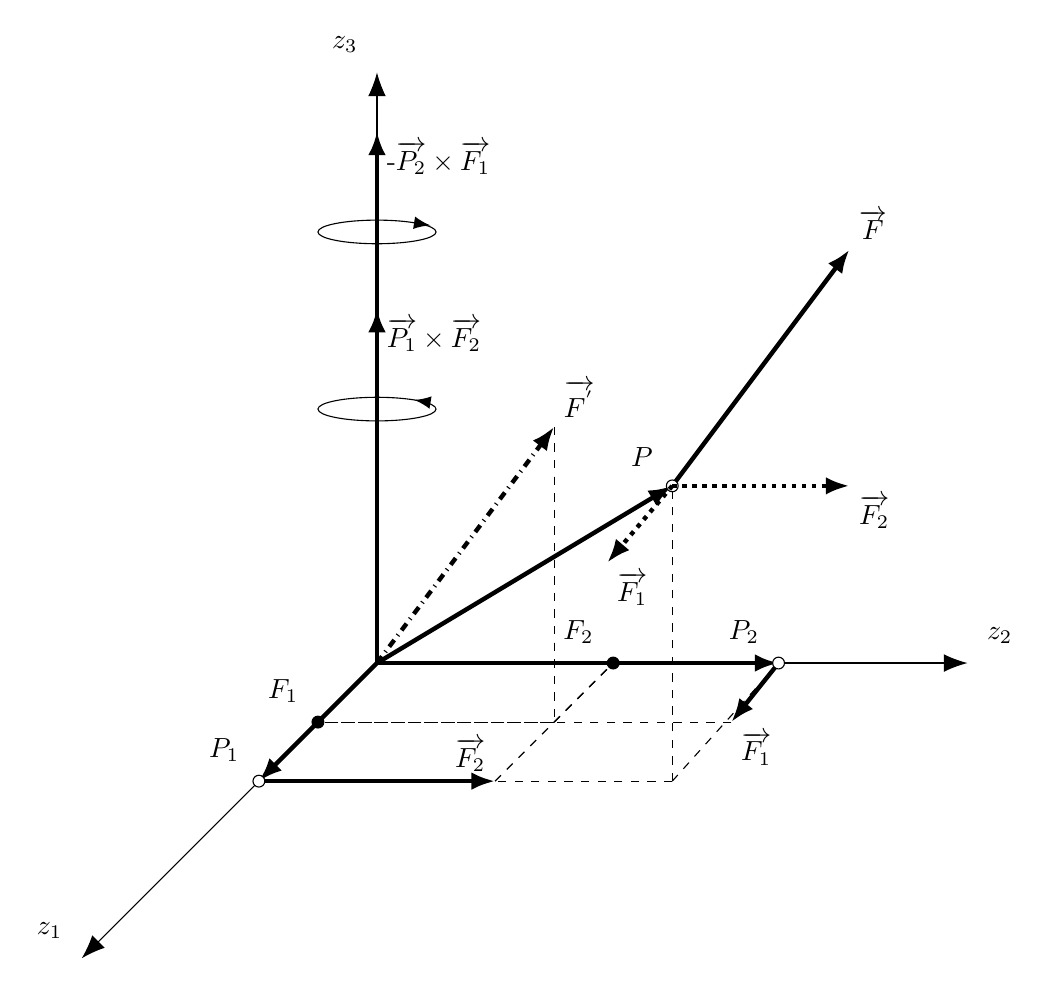
\begin{tikzpicture}[scale=0.75]
\tikzstyle{left-hand-mirror} = [
    draw,
    postaction=decorate, 
    decoration={
        markings,
        mark=between positions 0.015 and 0.98 step 0.1072 with {\draw (0,0)--(60:3pt);}
    }
]  
\coordinate (O) at (0,0);
\coordinate (X) at (-5,-5);
\coordinate (Y) at (10,0);
\coordinate (Z) at (0,10);
\draw [-{Latex[length=3mm]}] (O) -- (X);
\draw [-{Latex[length=3mm]}] (O) -- (Y);
\draw [-{Latex[length=3mm]}] (O) -- (Z);
\node[label=north west:$z_1$] at (X) {};
\node[label=north east:$z_2$] at (Y) {};
\node[label=north west:$z_3$] at (Z) {};
\coordinate (P) at (5,3);
\draw [-{Latex[length=3mm]},ultra thick] (O) -- (P);
\node[label=north west:$P$] at (P) {};
\coordinate (F) at (8,7) {};
\draw [-{Latex[length=3mm]}, ultra thick] (P) -- (F);
\node[above right] at (F) {$\overrightarrow{F}$};
\coordinate (Fp) at (8-5,7-3) {};
\draw [-{Latex[length=3mm]},dashdotted,ultra thick] (O) -- (Fp);
\node[above right,] at (Fp) {$\overrightarrow{F^{'}}$};
\coordinate (Px) at (-2,-2) {};
\coordinate (Py) at (6.8,0) {};
\node[label=north west:$P_1$] at (Px) {};
\node[label=north west:$P_2$] at (Py) {};
\coordinate (Pp) at (5,-2) {};
\draw [dashed] (Pp) -- (P);
\draw [dashed] (Pp) -- (Px);
\draw [dashed] (Pp) -- (Py);
\coordinate (Fpp) at (3,-1) {};
\coordinate (Fx) at (-1,-1) {} {};
\coordinate (Fy) at (4,0) {} {};
\node[label=north west:$F_1$] at (Fx) {};
\node[label=north west:$F_2$] at (Fy) {};
\draw[fill = black]  (Fx) circle (0.1);
\draw[fill = black]  (Fy) circle (0.1);
\draw [dashed] (Fp) -- (Fpp);
\draw [dashed] (Fpp) -- (Fx);
\draw [dashed] (Fpp) -- (Fy);

\coordinate (Fppp) at (6,-1) {} {};
\coordinate (Pppp) at (2,-2) {} {} {};
\node[{anchor=north west }] at (Fppp) {$\overrightarrow{F_1}$};
\node[{anchor=south east }] at (Pppp) {$\overrightarrow{F_2}$};
\draw [-{Latex[length=3mm]}, ultra thick] (O) -- (Px);
\draw [-{Latex[length=3mm]},ultra thick] (O) -- (Py);
\draw [-{Latex[length=3mm]}, ultra thick] (Px) -- (Pppp);
\draw [-{Latex[length=3mm]},ultra thick] (Py) -- (Fppp);
%\node[label=north west:$K$] at (Fppp) {};
%\node[label=north west:$S$] at (Pppp) {};
\draw [dashed] (Fp) -- (Fpp);
\draw [dashed] (Fppp) -- (Fx);
\draw [dashed] (Pppp) -- (Fy);
%\filldraw[ultra thick, gray!10] (Px) -- (Pppp) -- (Fy) -- (O) -- (Px) -- cycle;
%\filldraw[ultra thick,gray!20] (Fx) -- (Fppp) -- (Py) -- (O) -- (Px) -- cycle;
%\draw[ultra thick, gray!80] (Px) -- (Pppp) -- (Fy) -- (O) -- (Px) -- cycle;
%\draw[ultra thick,gray!80] (Fx) -- (Fppp) -- (Py) -- (O) -- (Px) -- cycle;
\coordinate (Vp1) at (0,6) {} {};
\coordinate (Vp2) at (0,9) {} {} {};
\draw [-{Latex[length=3mm]}, ultra thick] (O) -- (Vp1);
\draw [-{Latex[length=3mm]}, ultra thick] (O) -- (Vp2);
\node[{anchor=north west }] at (Vp1) {$\overrightarrow{P_1}\times\overrightarrow{F_2}$};
\node[{anchor=north west }] at (Vp2) {-$\overrightarrow{P_2}\times\overrightarrow{F_1}$};
\draw[fill=white]  (Py) circle (0.1);
\draw[fill=white]  (Px) circle (0.1);
\draw[fill=white]  (P) circle (0.1);
\draw[decoration={markings, mark=at position 0.1 with {\arrow[scale = 1.5]{latex[]}}},
    postaction={decorate}](0,4.3) ellipse (1 and 0.2);
    \draw[decoration={markings, mark=at position 0.1 with {\arrow[scale = 1.5]{latex[reversed]}}},
    postaction={decorate}](0,7.3) ellipse (1 and 0.2);
 \coordinate (Qx) at (3.9,1.7) {} {};
\coordinate (Qy) at (8,3) {} {} {};
\draw [-{Latex[length=3mm]},dotted, ultra thick] (P) -- (Qx);
\draw [-{Latex[length=3mm]},dotted, ultra thick] (P) -- (Qy);
\node[{anchor=north west }] at (Qx) {$\overrightarrow{F_1}$};
\node[{anchor=north west }] at (Qy) {$\overrightarrow{F_2}$};
\end{tikzpicture}
\caption{Interpretation of the tensor moment $M_{12}$}
\label{fig:fig_p156_5320}
\end{figure}
Let's consider a mass point $P$ on which a force $\overrightarrow{F}$ is acting. The force has components $\left(F_x,F_y,F_z\right)$ in the  space $V^{'}_3$ (which is by the way not the space $V_3$ of the considered mass point).\\
Let's investigate the element $M_{12}$ of the \textit{tensor moment}.\\
$P_1F_2\overrightarrow{e_3}$ is the vector product $\overrightarrow{P_1}\times\overrightarrow{F_2}$ and is as such the torque of the component $F_2$ of $\overrightarrow{F}$ acting on the mass point situated at $P_1$. The origin being fixed, $\overrightarrow{F_2}$ tries to move $P_1$, clockwise along the $z_3$ axis. The same is true for the component $\overrightarrow{F_1}$ acting on the mass point situated at $P_2$, and is represented here by the vector $- \overrightarrow{P_2}\times\overrightarrow{F_1}$ ($\overrightarrow{F_1}$ tries to move  $P_2$, counter clockwise along the $z_3$ axis). \\
Hence, $P_1F_2-P_2F_1$ is the net force trying to move the point $P$ along the $z_3$ axis (i.e. in the plane $\parallel$ with the $z_3=0$ plane).
$$\blacklozenge$$
\newpage


\section{p156 - Clarification to 5.234}
\begin{tcolorbox}
$$\mathbf{5.234.}\spatie \dv{h_r}{t}= M_r$$
\end{tcolorbox}
\begin{align}
h_r &= m\epsilon_{rmn}z_mv_n\\
\Rightarrow \spatie \dv{h_r}{t} &= m\epsilon_{rmn}\dv{z_m}{t} v_n+m\epsilon_{rmn}z_m\dv{v_n}{t}\\
&= m\underbrace{\epsilon_{rmn}v_m v_n}_{=0}+\underbrace{\epsilon_{rmn}z_mF_n}_{=M_r}\\
&=M_r
\end{align}
$$\blacklozenge$$
\newpage



\section{p158-159 - Clarification to 5.313}
\begin{tcolorbox}
$$\mathbf{5.313.}\spatie \omega_{rs}= -\omega_{sr}$$ From 5.310 and the vector character of $v_r$ and $z_r$ (for transformations which do not change the origin), \textbf{it follows that $\omega_{rs} $ is a Cartesian tensor of second order}.
\end{tcolorbox}
Be 
\begin{align}
v^{}_r = -\omega^{}_{rn}z^{}_n
\end{align}
Considering orthogonal transformation in a flat space $z^{'}_m = A_{mr}z^{}_r+B_m$ with  $B_m=0$ as we consider only transformations which do not change the origin. Differentiation with the parameter $t$ gives 
\begin{align}
v^{'}_m &= A_{mr}v^{}_r\\
&= -\omega^{}_{rn}A_{mr}z^{}_n\\
\end{align}
But $z^{'}_q = A_{qr}z^{}_r\quad\Rightarrow \quad A_{qn}z^{'}_q = A_{qn}A_{qr}z^{}_r\quad\Rightarrow \quad A_{qn}z^{'}_q = z^{}_n$ 
Hence
\begin{align}
v^{'}_m &= -\omega^{}_{rn}A_{mr}z^{}_n\\
&= -\underbrace{\omega^{}_{rn}A_{mr}A_{qn}}_{\overset{\underset{\mathrm{def}}{}}{=}\omega_{mq}^{'}}z^{'}_q\\
v^{'}_m &= -\omega_{mq}^{'}z^{'}_q
\end{align}
$$\blacklozenge$$
\newpage


\section{p159 - Exercise}
\begin{tcolorbox}
Show that if a rigid body rotates about the point $z_r=b_r$ as fixed point, the velocity of a general point of the body is given by $$v_r=-\omega_{rm}\left(z_m-b_m\right)$$
\end{tcolorbox}
By $\mathbf{5.302. }$:
\begin{align}
\left(z^{(1)}_m-z^{(2)}_m\right)\left(dz^{(1)}_m-dz^{(2)}_m\right)=0
\end{align}
At the fixed point we have $z^{(2)}_m=b_m$ and $dz^{(2)}_m=0$, hence
\begin{align}
\left(z^{(1)}_m-b_m\right)\left(dz^{(1)}_m\right)=0\\
\Rightarrow\spatie z^{(1)}_mdz^{(1)}_m =b_mdz^{(1)}_m
\end{align}
As this is true for any point of the rigid mass, expanding (1) and using (3) we get when dividing by $dt$
\begin{align}
\left(z^{(2)}_m-b_m\right)v^{(1)}_m+\left(z^{(1)}_m-b_m\right)v^{(2)}_m=0
\end{align}
Taking twice the partial derivative $\frac{\partial^2}{\partial z^{(1)}_p\partial z^{(1)}_q}$ we get
\begin{align}
\left(z^{(2)}_m-b_m\right)\frac{\partial^2 v_m}{\partial z^{(1)}_p\partial z^{(1)}_q}=0
\end{align}
As this is true for any arbitrary point in the rigid body we get
\begin{align}
\frac{\partial^2 v_m}{\partial z^{(1)}_p\partial z^{(1)}_q}=0\\
\Rightarrow\spatie v_m= K_{mr}z_r+B_m
\end{align}
At the fixed point we have 
\begin{align}
 K_{mr}b_r+B_m =0
\end{align}
Plugging this in (7)
\begin{align}
 v_m= K_{mr}\left(z_r-b_m\right)
\end{align}
Putting $K_{mr}=-\omega_{mr}$ gives us indeed the asked expression.
$$\blacklozenge$$
\newpage


\section{p161 - Clarification to 5.325 and 5.326}
\begin{tcolorbox}
$$\mathbf{5.325.}\spatie \Omega_{np}\sum \left(mf_nz_p\right)= \Omega_{np}\sum F_nz_p $$
and hence, since $\Omega_{np}$ is arbitrary,
$$\mathbf{5.326.}\spatie \sum m\left(f_nz_p-f_pz_n\right)= \sum \left(F_nz_p-F_pz_n \right)$$
\end{tcolorbox}
To be complete the following step should be inserted

\begin{align}
\Omega_{np}\sum \left(mf_nz_p\right)&= \Omega_{np}\sum F_nz_p \\
\text{As }\Omega_{np}\text{ is skew-symmetric:}\spatie -\Omega_{np}\sum \left(mf_pz_n\right)&= -\Omega_{np}\sum F_pz_n \\
\text{(1)+(2) }\spatie \Omega_{np}\sum m\left(f_nz_p-f_pz_n\right)&= \Omega_{np}\sum\left( F_nz_p -F_pz_n\right)
\end{align}
and hence, since $\Omega_{np}$ is arbitrary,
$$\mathbf{5.326.}\spatie \sum m\left(f_nz_p-f_pz_n\right)= \sum \left(F_nz_p-F_pz_n \right)$$
$$\blacklozenge$$
\newpage

\section{p161 - Clarification to 5.329 and 5.330}
\begin{tcolorbox}
$$\mathbf{5.329.}\spatie h_{np}=\sum m\left(\omega_{nq} z_q z_p -\omega_{pq} z_qz_n\right)$$
$$= J_{npqr}\omega_{rq}$$
where
$$\mathbf{5.330.}\spatie J_{npqr}= \sum m\left(\delta_{nr}z_qz_p-\delta_{pr}z_nz_q \right)$$
\end{tcolorbox}
\begin{align}
h_{np}&=\sum m\left(\omega_{nq} z_q z_p -\omega_{pq} z_qz_n\right)\\
&=\sum m\left(\omega_{rq}\delta_{rn} z_q z_p -\omega_{rq} \delta_{rp}z_qz_n\right)\\
&=\omega_{rq}\sum m\left(\delta_{rn} z_q z_p -\delta_{rp}z_qz_n\right)\\
&=J_{npqr}\omega_{rq}
\end{align}
$$\blacklozenge$$
\newpage


\section{p166 - Exercise}
\begin{tcolorbox}
Deduce immediately from $\mathbf{5.420.}$ that the Coriolis force is perpendicular to the velocity.
\end{tcolorbox}
\begin{align}
G^{'}_s &= 2m\omega^{'}_{sm}(S^{'},S)v^{'}_m(S^{'})\\
\times v^{'}_s(S^{'})\quad : \spatie G^{'}_s v^{'}_s(S^{'})&=m\left(\omega^{'}_{sm}(S^{'},S)v^{'}_m(S^{'})v^{'}_s(S^{'})+\omega^{'}_{ms}(S^{'},S)v^{'}_m(S^{'})v^{'}_s(S^{'})\right)\\
&=0\quad\text{as }\omega^{'}_{ms}\text{ is skew-symmetric}
\end{align}
$$\blacklozenge$$
\newpage

\section{p166 - Exercise}
\begin{tcolorbox}
Show that if $N=3$ and $\dot{\omega}^{'}_r(S^{'},S) =0$, then the centrifugal force may be written 
$$\mathbf{5.422.}\spatie C^{'}_s = m\omega^{'}_{n}(S^{'},S)\omega^{'}_{n}(S^{'},S)z^{'}_s-m\omega^{'}_{n}(S^{'},S)z^{'}_n\omega^{'}_{s}(S^{'},S)$$
Deduce that $ C^{'}_s$ is coplanar with the vectors $\omega^{'}_{s}(S^{'},S)$ and $z^{'}_n$ and perpendicular to the former.
\end{tcolorbox}
By $\mathbf{5.420.}$ with $\dot{\omega}^{'}_r(S^{'},S) =0$ and using $\mathbf{5.316.} \quad ( \omega^{'}_{rs}=\epsilon_{rsn}\omega^{'}_n)$
\begin{align}
C^{'}_s &= m\omega^{'}_{sm}(S^{'},S)\omega^{'}_{nm}(S^{'},S)z^{'}_n\\
&= m\epsilon_{smk}\omega^{'}_k(S^{'},S)\epsilon_{nmp}\omega^{'}_p(S^{'},S)z^{'}_n\\
&= m\epsilon_{msk}\epsilon_{mnp}\omega^{'}_k(S^{'},S)\omega^{'}_p(S^{'},S)z^{'}_n\\
&= m\left(\delta_{sn}\delta_{kp} -\delta_{sp}\delta_{kn} \right)\omega^{'}_k(S^{'},S)\omega^{'}_p(S^{'},S)z^{'}_n\\
&= m\delta_{sn}\delta_{kp}\omega^{'}_k(S^{'},S)\omega^{'}_p(S^{'},S)z^{'}_n -m\delta_{sp}\delta_{kn} \omega^{'}_k(S^{'},S)\omega^{'}_p(S^{'},S)z^{'}_n\\
&= m\omega^{'}_p(S^{'},S)\omega^{'}_p(S^{'},S)z^{'}_s - m\omega^{'}_n(S^{'},S)\omega^{'}_s(S^{'},S)z^{'}_n
\end{align}
To deduce that $ C^{'}_s$ is coplanar with the vectors $\omega^{'}_{s}(S^{'},S)$ and $z^{'}_n$ we calculate the mixed triple product
\begin{align}
P &= \epsilon_{spr}C^{'}_s \omega^{'}_p(S^{'},S)z^{'}_r\\
&= m\underbrace{\epsilon_{spr} \omega^{'}_n(S^{'},S)\omega^{'}_n(S^{'},S)z^{'}_s \omega^{'}_p(S^{'},S)z^{'}_r}_{=0} -\underbrace{ m\epsilon_{spr}\omega^{'}_n(S^{'},S)\omega^{'}_s(S^{'},S)z^{'}_n \omega^{'}_p(S^{'},S)z^{'}_r}_{=0}\\
=0
\end{align}
Both terms vanish: the first by the presence of the terms $\epsilon_{spr}z^{'}_s z^{'}_r$ which cancel each other and for the second by the terms $\epsilon_{spr}\omega^{'}_s(S^{'},S) \omega^{'}_p(S^{'},S)$. As $P=0$, the three vectors are coplanar.\\
We now calculate the inner product $C^{'}_s\omega^{'}_s(S^{'},S)$
\begin{align}
P&= m\omega^{'}_n(S^{'},S)\omega^{'}_n(S^{'},S)z^{'}_s\omega^{'}_s(S^{'},S) - \underbrace{m\omega^{'}_n(S^{'},S)\omega^{'}_s(S^{'},S)z^{'}_n\omega^{'}_s(S^{'},S)}_{\Leftrightarrow \  m\omega^{'}_n(S^{'},S)\omega^{'}_n(S^{'},S)z^{'}_s\omega^{'}_s(S^{'},S)}\\
&=0
\end{align}
$$\blacklozenge$$
\newpage

\section{p168 - Exercise}
\begin{tcolorbox}
Taking $N=3$, show that $\mathbf{5.424}$ may be reduced to the usual Euler equations:
$$ I_{11}\dv{\omega^{'}_1(S^{'},S)}{t}-\left(I_{22}-I^{'}_{33}\right)\omega^{}_2(S^{'},S)\omega^{'}_3(S^{'},S)=M^{'}_1$$ and two similar equations.
\end{tcolorbox}
We first begin with an approach which leads to nothing. I probably made a reasoning error. I give here the whole calculation as this was interesting and also to, later, find my mistake. After this buggy solution, I will give a second version, which works.\\\\
$\mathbf{5.424}$:
\begin{align}
M^{'}_{ab}&=J^{'}_{abrq}\dv{\omega^{'}_{rq}(S^{'},S)}{t}+J^{'}_{cdrq}\left(\delta_{ac}\delta_{du}\delta_{bv}+\delta_{bd}\delta_{cu}\delta_{av}\right)\omega^{'}_{rq}(S^{'},S)\omega^{'}_{uv}(S^{'},S) =\\
\times \epsilon_{sab} \text{: }\quad 2M^{'}_{s}&=\epsilon_{sab }J^{'}_{abrq}\dv{\omega^{'}_{rq}(S^{'},S)}{t}+\epsilon_{sab}J^{'}_{cdrq}\left(\delta_{ac}\delta_{du}\delta_{bv}+\delta_{bd}\delta_{cu}\delta_{av}\right)\omega^{'}_{rq}(S^{'},S)\omega^{'}_{uv}(S^{'},S) 
\end{align}
Using $ \omega^{'}_{rq}(S^{'},S)= \epsilon_{rqt}\omega^{'}_{t}(S^{'},S)$ and $I_{st}=\half J^{'}_{abrq}\epsilon_{abs}\epsilon_{rqt}$
\begin{align}
2M^{'}_{s}&=2I_{st}\dv{\omega^{'}_{t}(S^{'},S)}{t}+\epsilon_{sab}\epsilon_{rqi}\epsilon_{uvj}J^{'}_{cdrq}\left(\delta_{ac}\delta_{du}\delta_{bv}+\delta_{bd}\delta_{cu}\delta_{av}\right)\omega^{'}_{i}(S^{'},S)\omega^{'}_{j}(S^{'},S) \\
&=\left\{\begin{array}{l}
2I_{st}\dv{\omega^{'}_{t}(S^{'},S)}{t}\\\\ + \left(\epsilon_{sab}\epsilon_{rqi}\epsilon_{uvj}J^{'}_{cdrq}\delta_{ac}\delta_{du}\delta_{bv}+\epsilon_{sab}\epsilon_{rqi}\epsilon_{uvj}J^{'}_{cdrq}\delta_{bd}\delta_{cu}\delta_{av}\right)\omega^{'}_{i}(S^{'},S)\omega^{'}_{j}(S^{'},S) 
\end{array}\right.\\
&=\left\{\begin{array}{l}
2I_{st}\dv{\omega^{'}_{t}(S^{'},S)}{t}\\\\ + \left(\epsilon_{scb}\epsilon_{rqi}\epsilon_{dbj}J^{'}_{cdrq}+\epsilon_{sad}\epsilon_{rqi}\epsilon_{caj}J^{'}_{cdrq}\right)\omega^{'}_{i}(S^{'},S)\omega^{'}_{j}(S^{'},S) 
\end{array}\right.\\
&=\left\{\begin{array}{l}
2I_{st}\dv{\omega^{'}_{t}(S^{'},S)}{t}\\\\ + \left(\epsilon_{bcs}\epsilon_{bdj}\right)\epsilon_{rqi}J^{'}_{cdrq}\omega^{'}_{i}(S^{'},S)\omega^{'}_{j}(S^{'},S) \\\\+\left(\epsilon_{asd}\epsilon_{acj}\right)\epsilon_{rqi}J^{'}_{cdrq}\omega^{'}_{i}(S^{'},S)\omega^{'}_{j}(S^{'},S) 
\end{array}\right.\\
&=\left\{\begin{array}{l}
2I_{st}\dv{\omega^{'}_{t}(S^{'},S)}{t}\\\\ + \left(\delta_{cd}\delta_{sj}-\delta_{cj}\delta_{sd}\right)\epsilon_{rqi}J^{'}_{cdrq}\omega^{'}_{i}(S^{'},S)\omega^{'}_{j}(S^{'},S) \\\\+\left(\delta_{sc}\delta_{dj}-\delta_{sj}\delta_{dc}\right)\epsilon_{rqi}J^{'}_{cdrq}\omega^{'}_{i}(S^{'},S)\omega^{'}_{j}(S^{'},S) 
\end{array}\right.
\end{align}
\begin{align}
&=\left\{\begin{array}{l}
2I_{st}\dv{\omega^{'}_{t}(S^{'},S)}{t}\\\\ +\epsilon_{rqi}J^{'}_{ccrq}\omega^{'}_{i}(S^{'},S)\omega^{'}_{s}(S^{'},S) \\\\
-\epsilon_{rqi}J^{'}_{jsrq}\omega^{'}_{i}(S^{'},S)\omega^{'}_{j}(S^{'},S) \\\\+\epsilon_{rqi}J^{'}_{sjrq}\omega^{'}_{i}(S^{'},S)\omega^{'}_{j}(S^{'},S) 
\\\\-\epsilon_{rqi}J^{'}_{ccrq}\omega^{'}_{i}(S^{'},S)\omega^{'}_{s}(S^{'},S)
\end{array}\right.
\end{align}
giving
\begin{align}
2M^{'}_{s}&=\left\{\begin{array}{l}
2I_{st}\dv{\omega^{'}_{t}(S^{'},S)}{t} 
\\\\+\epsilon_{rqi}J^{'}_{sjrq}\omega^{'}_{i}(S^{'},S)\omega^{'}_{j}(S^{'},S)
\\\\
-\epsilon_{rqi}J^{'}_{jsrq}\omega^{'}_{i}(S^{'},S)\omega^{'}_{j}(S^{'},S)  
\end{array}\right.
\end{align}
For $s=1$:
\begin{table}[H]
\centering
 \begin{tabular}{||c | | c  | c||} 
 \hline
  & $+\epsilon_{rqi}J^{}_{1jrq}\omega^{}_{i}\omega^{}_{j}$ & $-\epsilon_{rqi}J^{}_{j1rq}\omega^{}_{i}\omega^{}_{j}   $\\ [1.5ex] 
 \hline\hline
 $\epsilon_{123}$ & $+J^{}_{1112}\omega^{}_{3}\omega^{}_{1}+J^{}_{1212}\omega^{}_{3}\omega^{}_{2}+J^{}_{1312}\omega^{}_{3}\omega^{}_{3}$ & $-J^{}_{1112}\omega^{}_{3}\omega^{}_{1}-J^{}_{2112}\omega^{}_{3}\omega^{}_{2}-J^{}_{3112}\omega^{}_{3}\omega^{}_{3}   $\\  
 $\epsilon_{132}$ & $-J^{}_{1113}\omega^{}_{2}\omega^{}_{1}-J^{}_{1213}\omega^{}_{2}\omega^{}_{2}-J^{}_{1313}\omega^{}_{2}\omega^{}_{3}$ & $+J^{}_{1113}\omega^{}_{2}\omega^{}_{1} +J^{}_{2113}\omega^{}_{2}\omega^{}_{2} +J^{}_{3113}\omega^{}_{2}\omega^{}_{3}   $\\
 $\epsilon_{213}$ & $-J^{}_{1121}\omega^{}_{3}\omega^{}_{1}-J^{}_{1221}\omega^{}_{3}\omega^{}_{2}-J^{}_{1321}\omega^{}_{3}\omega^{}_{3}$ & $+J^{}_{1121}\omega^{}_{3}\omega^{}_{1}+J^{}_{2121}\omega^{}_{3}\omega^{}_{2}+J^{}_{3121}\omega^{}_{3}\omega^{}_{3}   $\\
 $\epsilon_{231}$ & $+J^{}_{1123}\omega^{}_{1}\omega^{}_{1}+J^{}_{1223}\omega^{}_{1}\omega^{}_{2}+J^{}_{1323}\omega^{}_{1}\omega^{}_{3}$ & $-J^{}_{1123}\omega^{}_{1}\omega^{}_{1}-J^{}_{2123}\omega^{}_{1}\omega^{}_{2}-J^{}_{3123}\omega^{}_{1}\omega^{}_{3}   $\\
 $\epsilon_{321}$ & $-J^{}_{1132}\omega^{}_{1}\omega^{}_{1}-J^{}_{1232}\omega^{}_{1}\omega^{}_{2}-J^{}_{1332}\omega^{}_{1}\omega^{}_{3}$ & $+J^{}_{1132}\omega^{}_{1}\omega^{}_{1}  +J^{}_{2132}\omega^{}_{1}\omega^{}_{2}  +J^{}_{3132}\omega^{}_{1}\omega^{}_{3}   $\\
 $\epsilon_{312}$ & $+J^{}_{1131}\omega^{}_{2}\omega^{}_{1}+J^{}_{1231}\omega^{}_{2}\omega^{}_{2}+J^{}_{1331}\omega^{}_{2}\omega^{}_{3}$ & $-J^{}_{1131}\omega^{}_{2}\omega^{}_{1} -J^{}_{2131}\omega^{}_{2}\omega^{}_{2} -J^{}_{3131}\omega^{}_{2}\omega^{}_{3}   $\\   [1ex] 
 \hline
 \end{tabular}
\end{table}

Taking into account that $J^{}_{abcd}=0$ for $a\ne c  \wedge b\ne d$

\begin{table}[H]
\centering
 \begin{tabular}{||c | | c  | c||} 
 \hline
  & $+\epsilon_{rqi}J^{}_{1jrq}\omega^{}_{i}\omega^{}_{j}$ & $-\epsilon_{rqi}J^{}_{j1rq}\omega^{}_{i}\omega^{}_{j}   $\\ [1.5ex] 
 \hline\hline
 $\epsilon_{123}$ & $+\cancel{J^{}_{1112}\omega^{}_{3}\omega^{}_{1}}+J^{}_{1212}\omega^{}_{3}\omega^{}_{2}+J^{}_{1312}\omega^{}_{3}\omega^{}_{3}$ & $-\cancel{J^{}_{1112}\omega^{}_{3}\omega^{}_{1}} $\\  
 $\epsilon_{132}$ & $-\cancel{J^{}_{1113}\omega^{}_{2}\omega^{}_{1}}-J^{}_{1213}\omega^{}_{2}\omega^{}_{2}-J^{}_{1313}\omega^{}_{2}\omega^{}_{3}$ & $+\cancel{J^{}_{1113}\omega^{}_{2}\omega^{}_{1} } $\\
 $\epsilon_{213}$ & $-\cancel{J^{}_{1121}\omega^{}_{3}\omega^{}_{1}}$ & $+\cancel{J^{}_{1121}\omega^{}_{3}\omega^{}_{1}}+J^{}_{2121}\omega^{}_{3}\omega^{}_{2}+J^{}_{3121}\omega^{}_{3}\omega^{}_{3}   $\\
 $\epsilon_{231}$ & $+J^{}_{1323}\omega^{}_{1}\omega^{}_{3}$ & $-J^{}_{2123}\omega^{}_{1}\omega^{}_{2}$\\
 $\epsilon_{321}$ & $-J^{}_{1232}\omega^{}_{1}\omega^{}_{2}$ & $+J^{}_{3132}\omega^{}_{1}\omega^{}_{3}   $\\
 $\epsilon_{312}$ & $+\cancel{J^{}_{1131}\omega^{}_{2}\omega^{}_{1}}$ & $-\cancel{J^{}_{1131}\omega^{}_{2}\omega^{}_{1}} -J^{}_{2131}\omega^{}_{2}\omega^{}_{2} -J^{}_{3131}\omega^{}_{2}\omega^{}_{3}   $\\   [1ex] 
 \hline
 \end{tabular}
\end{table}
Opposite sign terms vanish, giving
\begin{table}[H]
\centering
 \begin{tabular}{||c | | c  | c||} 
 \hline
  & $+\epsilon_{rqi}J^{}_{1jrq}\omega^{}_{i}\omega^{}_{j}$ & $-\epsilon_{rqi}J^{}_{j1rq}\omega^{}_{i}\omega^{}_{j}   $\\ [1.5ex] 
 \hline\hline
 $\epsilon_{123}$ & $+J^{}_{1212}\omega^{}_{3}\omega^{}_{2}+J^{}_{1312}\omega^{}_{3}\omega^{}_{3}$ & $ $\\  
 $\epsilon_{132}$ & $-J^{}_{1213}\omega^{}_{2}\omega^{}_{2}-J^{}_{1313}\omega^{}_{2}\omega^{}_{3}$ & $ $\\
 $\epsilon_{213}$ & $ $ & $+J^{}_{2121}\omega^{}_{3}\omega^{}_{2}+J^{}_{3121}\omega^{}_{3}\omega^{}_{3}   $\\
 $\epsilon_{231}$ & $+J^{}_{1323}\omega^{}_{1}\omega^{}_{3}$ & $-J^{}_{2123}\omega^{}_{1}\omega^{}_{2}$\\
 $\epsilon_{321}$ & $-J^{}_{1232}\omega^{}_{1}\omega^{}_{2}$ & $+J^{}_{3132}\omega^{}_{1}\omega^{}_{3}   $\\
 $\epsilon_{312}$ & $ $ & $-J^{}_{2131}\omega^{}_{2}\omega^{}_{2} -J^{}_{3131}\omega^{}_{2}\omega^{}_{3}   $\\   [1ex] 
 \hline
 \end{tabular}
\end{table}
Considering $J_{abcd}= -J_{badc}$
\begin{table}[H]
\centering
 \begin{tabular}{||c | | c  | c||} 
 \hline
  & $+\epsilon_{rqi}J^{}_{1jrq}\omega^{}_{i}\omega^{}_{j}$ & $-\epsilon_{rqi}J^{}_{j1rq}\omega^{}_{i}\omega^{}_{j}   $\\ [1.5ex] 
 \hline\hline
 $\epsilon_{123}$ & $+\cancel{J^{}_{1212}}\omega^{}_{3}\omega^{}_{2}+\cancel{J^{}_{1312}}\omega^{}_{3}\omega^{}_{3}$ & $ $\\  
 $\epsilon_{132}$ & $-\cancel{J^{}_{1213}}\omega^{}_{2}\omega^{}_{2}-\cancel{J^{}_{1313}}\omega^{}_{2}\omega^{}_{3}$ & $ $\\
 $\epsilon_{213}$ & $ $ & $+\cancel{J^{}_{2121}}\omega^{}_{3}\omega^{}_{2}+\cancel{J^{}_{3121}}\omega^{}_{3}\omega^{}_{3}   $\\
 $\epsilon_{231}$ & $+\cancel{J^{}_{1323}}\omega^{}_{1}\omega^{}_{3}$ & $-\cancel{J^{}_{2123}}\omega^{}_{1}\omega^{}_{2}$\\
 $\epsilon_{321}$ & $-\cancel{J^{}_{1232}}\omega^{}_{1}\omega^{}_{2}$ & $+\cancel{J^{}_{3132}}\omega^{}_{1}\omega^{}_{3}   $\\
 $\epsilon_{312}$ & $ $ & $-\cancel{J^{}_{2131}}\omega^{}_{2}\omega^{}_{2} -\cancel{J^{}_{3131}}\omega^{}_{2}\omega^{}_{3}   $\\   [1ex] 
 \hline
 \end{tabular}
\end{table}

We get $$ m^{'}_s = I_{st}\dv{\omega^{'}_{t}(S^{'},S)}{t}$$?????\\
$$\lozenge$$\\
\newpage
Let's try another approach. Start with $\mathbf{5.332.}$: $\dv{}{t}\left(I_{st}\omega_{t}\right)= M_s$
\begin{align}
\dv{}{t}\left(I_{st}(S^{'},S)\omega_{t}(S^{'},S)\right)= M_s(S^{'},S)
\end{align}
Cf. $\mathbf{5.408.}$
\begin{align}
\omega^{'}_{u}(S^{'},S)&=A_{uq}\omega^{}_{q}(S^{'},S)\\
\times A_{ut}\quad \rightarrow \spatie A_{ut}\omega^{'}_{u}(S^{'},S)&=A_{ut}A_{uq}\omega^{}_{q}(S^{'},S)\\
&=\omega^{}_{t}(S^{'},S)\\
\spatie \omega^{}_{t}(S^{'},S) &=  A_{ut}\omega^{'}_{u}(S^{'},S)\\
\textbf{(10)}\quad\Rightarrow\spatie M_s(S^{'},S) &=\dv{}{t}\left(I_{st}(S^{'},S)A_{ut}\omega^{'}_{u}(S^{'},S)\right)\\
\times A_{ps}\quad \Rightarrow M^{'}_p(S^{'},S) &=A_{ps}\dv{}{t}\left(I_{st}(S^{'},S)A_{ut}\omega^{'}_{u}(S^{'},S)\right)\\
I_{st}(S^{'},S)&= A_{as}A_{bt}I^{'}_{ab}(S^{'},S)\\
\textbf{(16)}\quad\Rightarrow \spatie M^{'}_p(S^{'},S) &=A_{ps}\dv{}{t}\left(A_{as}A_{bt}I^{'}_{ab}(S^{'},S)A_{ut}\omega^{'}_{u}(S^{'},S)\right)\\
&=A_{ps}\dv{}{t}\left(A_{as}I^{'}_{ak}(S^{'},S)\omega^{'}_{k}(S^{'},S)\right)
\end{align}
As we transformed $I_{st}(S^{'},S)$ to a coordinate system fixed to the body we have that the elements of $I^{'}_{ab}(S^{'},S)$ are constants.\\
Hence,
\begin{align}
 M^{'}_p(S^{'},S) &=I^{'}_{ak}S^{'},S)A_{ps}\dv{}{t}\left( A_{as}\omega^{'}_{k}(S^{'},S)\right)\\
 &=I^{'}_{ak}(S^{'},S)A_{ps}\left(\dot{A}_{as}\omega^{'}_{k}(S^{'},S)+A_{as} \dot{\omega}^{'}_{k}(S^{'},S)\right)\\
 &=I^{'}_{ak}(S^{'},S)A_{ps}A_{as} \dot{\omega}^{'}_{k}(S^{'},S)+ I^{'}_{ak}(S^{'},S)A_{ps}\dot{A}_{as}\omega^{'}_{k}(S^{'},S)\\
 &=I^{'}_{pk}(S^{'},S) \dot{\omega}^{'}_{k}(S^{'},S)+ I^{'}_{ak}(S^{'},S)A_{ps}\dot{A}_{as}\omega^{'}_{k}(S^{'},S)\\
\textbf{5.408.}\quad\Rightarrow \spatie  A_{ps}\dot{A}_{as} &= \omega^{'}_{ap}(S^{'},S)\\
\textbf{(23)}\quad\Rightarrow \spatie  M^{'}_p(S^{'},S) &=I^{'}_{pk}(S^{'},S) \dot{\omega}^{'}_{k}(S^{'},S)+ I^{'}_{ak}(S^{'},S)\omega^{'}_{ap}(S^{'},S)\omega^{'}_{k}(S^{'},S)
\end{align}
Let's now calculate the last expression for $p=1$
\begin{align}
M^{'}_1(S^{'},S) &=I^{'}_{1k}(S^{'},S) \dot{\omega}^{'}_{k}(S^{'},S)+ I^{'}_{ak}(S^{'},S)\omega^{'}_{a1}(S^{'},S)\omega^{'}_{k}(S^{'},S)
\end{align}
As we want an arbitrary, fixed to the body of course, coordinate system, it is possible to chose one so that the $I^{'}_{kj}(S^{'},S) = 0 $ for $k\neq j$ i.e. $I^{'}_{kj}(S^{'},S) $ is diagonal. This is possible because $ I^{'}_{kj}(S^{'},S) $ is symmetric (the finite-dimensional spectral theorem says that any symmetric matrix whose entries are real can be diagonalized by an orthogonal matrix).\\
We get, noticing that $\omega^{'}_{ab}(S^{'},S)$ is skew-symmetric and hence $\omega^{'}_{11}(S^{'},S) = 0$ :
\begin{align}
M^{'}_1(S^{'},S) &= I^{'}_{11}(S^{'},S) \dot{\omega}^{'}_{1}(S^{'},S)+ I^{'}_{22}(S^{'},S)\omega^{'}_{21}(S^{'},S)\omega^{'}_{2}(S^{'},S)+ I^{'}_{33}(S^{'},S)\omega^{'}_{31}(S^{'},S)\omega^{'}_{3}(S^{'},S)
\end{align}
Using $\mathbf{5.317}$:  $\omega^{'}_{21}(S^{'},S)=-\omega^{'}_{3}(S^{'},S)$ and $\omega^{'}_{31}(S^{'},S)=\omega^{'}_{2}(S^{'},S)$  we get the asked expression 
\begin{align}
M^{'}_1(S^{'},S) &= I^{'}_{11}(S^{'},S) \dot{\omega}^{'}_{1}(S^{'},S)-\left( I^{'}_{22}(S^{'},S)- I^{'}_{33}(S^{'},S)\right)\omega^{'}_{2}(S^{'},S)\omega^{'}_{3}(S^{'},S)
\end{align}
$$\blacklozenge$$
\newpage


\section{p169 - Exercise}
\begin{tcolorbox}
Assign convenient generalized coordinates for the three systems $(a), \ (b),\text{ and } (c)$ mentioned at the beginning of this section, and calculate the kinematical metric form in each case
\end{tcolorbox}
\textbf{$(a)$ a particle on a surface $(N=2)$}\\
No need here for fancy general coordinates: the $V_2$ coordinate system in the plane is the metric form of choice.
Indeed $\left|v\right|^2 = a_{mn}v_mv_n$ and for a $V_2$
$$ds^2 =\left(a_{11}\left(v^1\right)^2+2a_{12}v^1v^2+a_{22}\left(v^2\right)^2 \right)dt^2$$ and if the space is Euclidean and the plane smooth, we can choose an orthogonal system where $a_{12}$ will vanish.\\\\  
\textbf{$(b)$ a rigid body which can turn about a fixed point, as in the preceding section $(N=3)$}\\
For a rigid body we can choose a coordinate system $S^{'}$ fixed to the body to describe the geometry of the rigid body. The kinetic energy  referenced to a 'non-moving' (abuse of language) coordinate system $S$ is 
\begin{align}
T = \half\mathbf{\sum}\rho v^{'}_n(S)v^{'}_n(S)\spatie\text{(summation over all masses in the rigid body)}
\end{align}
We know by $\mathbf{5.409}$: $v^{'}_n(S)= v^{'}_n(S^{'})+ \omega^{'}_{mn}(S^{'},S)z^{'}_m$. As the $v^{'}_n(S^{'})$ are fixed, we have $v^{'}_n(S^{'})=0$ giving 
\begin{align}
T = \half\mathbf{\sum}\rho z^{'}_mz^{'}_k\omega^{'}_{mn}(S^{'},S)\omega^{'}_{kn}(S^{'},S)
\end{align}
Note in (2) that we bring $\omega^{'}_{mn}(S^{'},S)$ out of the summation as this expression  is the same for all masses in the body.
\begin{align}
\omega_{mn}(S^{'},S)&= \epsilon_{mnt}\omega^{'}_{t}(S^{'},S)\\
\Rightarrow\quad  
T &= \half\mathbf{\sum}\rho \epsilon_{mnt}\epsilon_{kns}z^{'}_mz^{'}_k\omega^{'}_{t}(S^{'},S)\omega^{'}_{s}(S^{'},S)\\
&= \half\mathbf{\sum}\rho \left(\delta_{mk}\delta_{ts}-\delta_{ms}\delta_{kt}\right)z^{'}_mz^{'}_k\omega^{'}_{t}(S^{'},S)\omega^{'}_{s}(S^{'},S)\\
&= \half\mathbf{\sum}\rho \left(z^{'}_mz^{'}_m\omega^{'}_{t}(S^{'},S)\omega^{'}_{t}(S^{'},S)-z^{'}_sz^{'}_t\omega^{'}_{t}(S^{'},S)\omega^{'}_{s}(S^{'},S)\right)\\
&= \half\mathbf{\sum}\rho \left(\delta_{st}z^{'}_mz^{'}_m\omega^{'}_{s}(S^{'},S)\omega^{'}_{t}(S^{'},S)-z^{'}_sz^{'}_t\omega^{'}_{t}(S^{'},S)\omega^{'}_{s}(S^{'},S)\right)\\
&= \half\mathbf{\sum}\rho \left(\delta_{st}z^{'}_mz^{'}_m-z^{'}_sz^{'}_t\right)\omega^{'}_{s}(S^{'},S)\omega^{'}_{t}(S^{'},S)
\end{align}
By $\mathbf{5.335.}$ we have $ I_{st} = \delta_{st}\mathbf{\sum}\rho z_mz_m-\mathbf{\sum}\rho z_sz_t$ and so (8) can be written as
\begin{align}
T&=\half I_{st}\omega^{'}_{s}(S^{'},S)\omega^{'}_{t}(S^{'},S)
\end{align} 
So we can choose the three angles $\Omega^{'}_{s}(S^{'},S)$  with ($\omega^{'}_{s}(S^{'},S)= \dv{\Omega^{'}_{s}(S^{'},S)}{t}$) as generalized coordinates and define $$ds^2=I_{st}d\Omega^{'}_{s}(S^{'},S)d\Omega^{'}_{t}(S^{'},S)$$ with  $$a_{mn} = I_{mn}$$ having constants as elements.
Some check on consistency of the metric tensor defined by $(14)$:\\
\textbf{Positive definite ?} : Yes, as $T$ is positive by construction.\\
\textbf{Symmetric ?} : Yes, as $a_{mn} = I_{km}$ and $I_{km}$ is symmetric.  \\
\begin{comment}
For a rigid body we can choose a coordinate system fixed to the body to describe the geometry of the rigid body. The kinetic energy is referenced to a 'fixed' coordinate system 
\begin{align}
T = \half\mathbf{\sum}\rho v_nv_n\spatie\text{summation over all masses in the rigid body}
\end{align}
as $z_n$ are fixed in the choose coordinate system it is clear that 
we have to find another way the express the velocity of the masses.

We know $v_n= - \omega_{nm}z_m$. As the $z_m$ are fixed, the only way the kinetic energy can change (and have 'a path' in the general coordinate system) is when $\omega_{nm}$ changes. 
We can write
\begin{align}
dT &=\half\mathbf{\sum}\rho  d\left(v_nv_n\right)\\
&=\half \mathbf{\sum}\rho  d\left(\omega_{nm}\omega_{nk}z_mz_k\right)\\
&=\half \mathbf{\sum}\rho  \left(\omega_{nk}d\omega_{nm}+\omega_{nm}d\omega_{nk}\right)z_mz_k\\
&= \left( \mathbf{\sum}\rho  \omega_{nm}z_mz_k\right)d\omega_{nk}
\end{align}
Note in (5) that we bring $d\omega_{nk}$ out of the summation as $\omega_{nk}$ is the same for all masses in the body.
As $dT$ can be negative we calculate $dT^2$
\begin{align}
dT^2&=\left( \mathbf{\sum}\rho  \omega_{nm}z_mz_k\right)\left( \mathbf{\sum}\rho  \omega_{pq}z_qz_r\right)d\omega_{nk}d\omega_{pr}\end{align}
\begin{align}
\omega_{nm}&= \epsilon_{nma}\omega_a\\
\Rightarrow\quad  
dT^2&=\left( \mathbf{\sum}\rho  \epsilon_{nma}\omega_az_mz_k\right)\left( \mathbf{\sum}\rho  \epsilon_{pqb}\omega_bz_qz_r\right)d\left(\epsilon_{nku}\omega_{u}\right)d\left(\epsilon_{prv}\omega_{v}\right)\\
&=\left( \mathbf{\sum}\rho  \epsilon_{nma}\epsilon_{nku}\omega_az_mz_k\right)\left( \mathbf{\sum}\rho  \epsilon_{pqb}\epsilon_{prv}\omega_bz_qz_r\right)d\omega_{u}\\
&=\left\{\begin{array}{l}\left( \mathbf{\sum}\rho  \left(\delta_{mk}\delta_{au}-\delta_{mu}\delta_{ak}\right)\omega_az_mz_k\right)d\omega_{u}\\ \left( \mathbf{\sum}\rho  \left(\delta_{qr}\delta_{bv}-\delta_{qv}\delta_{rb}\right)\omega_bz_qz_r\right)d\omega_{v}d\omega_{v}\\
\end{array}\right.\\
&=\left( \mathbf{\sum}\rho  \left(\omega_uz_nz_n-\omega_kz_uz_k\right)\right)\left( \mathbf{\sum}\rho  \left(\omega_vz_nz_n-\omega_rz_vz_r\right)\right)d\omega_{u} d\omega_{v}\\
&=\left( \mathbf{\sum}\rho  \left(\delta_{ku}\omega_kz_nz_n-\omega_kz_uz_k\right)\right)\left( \mathbf{\sum}\rho  \left(\delta_{rv}\omega_rz_nz_n-\omega_rz_vz_r\right)\right)d\omega_{u} d\omega_{v}\\
&=\left( \mathbf{\sum}\rho  \left(\delta_{ku}z_nz_n-z_uz_k\right)\right)\left( \mathbf{\sum}\rho  \left(\delta_{rv}z_nz_n-z_vz_r\right)\right)\omega_k\omega_rd\omega_{u} d\omega_{v}
\end{align}
By $\mathbf{5.335.}$ we have $ I_{ku} = \delta_{ku}\mathbf{\sum}\rho z_nz_n-\mathbf{\sum}\rho z_uz_k$ and so (13) can be written as
\begin{align}
dT^2&=I_{ku}I_{rv}\omega_k\omega_rd\omega_{u} d\omega_{v}
\end{align} 
So we can choose the three $\omega_k$ as generalized coordinates and define $$ds^2=a_{mn}d\omega_{m} d\omega_{n}$$ with  $$a_{mn} = I_{km}I_{rn}\omega_k \omega_r$$
The metric tensor $a_{mn}$ contains elements depending on the $\omega_k$ chosen as general coordinates of the system and is a good candidate as metric tensor.
Some check on consistency of the metric tensor defined by $(14)$:\\
\textbf{Positive definite ?} : Yes, as $dT^2$ is positive.\\
\textbf{Symmetric ?} : Yes, as $a_{mn} = I_{km}I_{rn}\omega_k \omega_r = I_{rn}I_{km}\omega_k \omega_r= a_{nm}$\\
\end{comment}
\\\\ \textbf{$(c)$ a chain of six rods smoothly hinged together, with one end fixed and all moving on a smooth plane $(N=6)$}\\

To simplify the notation we will assume that the mass $m_k$ of each rod (with length $L_k$) is concentrated at it's endpoint .\\
First we note that the velocity of a rod is composed of two vectors, one (labelled as $\overline{\nu}_k$) generated by its own rotation relative to the previous rod and the other (labelled as $\overline{v}_{k-1}$) generated by the velocity of the endpoint of the rod to which it is attached (see.fig. 5.2).
\begin{figure}[H]
    \centering
    \subfloat[]{\begin{tikzpicture}

\coordinate (p1) at (-0.5,2.5) {};
\draw[fill=white]  (p1) circle (0.1);
\coordinate (p2) at (-2.5,-2) {} {};
\draw[fill=white]  (p2) circle (0.1);
\coordinate (p12) at (-1.5,0) {} {} {};

\draw []  (p1) -- (p2);
\draw [dashed](-4.3302,-0.6) arc (-140.0002:-80:5);
\coordinate (p3) at (-0.5,-3.5) {} {};
\draw [dashdotted]  (p1) -- (p3);
\coordinate (v1) at (1.5,0.5) {} {} {};
\coordinate (v2) at (0.5,-3.5) {} {} {};
\coordinate (v3) at(-0.5,-4) {} {} {};
\coordinate (v4) at(-0.5+3,-4-1.5) {} {} {};
\draw [-{Latex[length=2mm]},very thick]  (p1) -- (v1);
\draw [-{Latex[length=2mm]},very thick]  (p2) -- (v2);
\draw [-{Latex[length=2mm]},very thick, dashed]  (p2) -- (v3);
\draw [-{Latex[length=2mm]},, dashed]  (p2) -- (v4);
\draw [ dotted]  (v2) -- (v4);
\draw [ dotted]  (v3) -- (v4);
\draw [dashed, decoration={markings, mark=at position 0.52 with {\arrow[scale = 1.]{Latex[length=2mm]}}},    postaction={decorate}](p12) arc [start angle=65,
        end angle=90,
        x radius=-2cm,
        y radius =-2cm];
\node[label=north east:$m_{k-1}$] at (p1) {};
\node[label=south west:$m_{k}$] at (p2) {};
\node[label=north east :$\theta_k$] at (p12) {};
\node[label=north west :$L_k$] at (p12) {};
\node[label=north east :$\overline{v}_{k-1}$] at (v1) {};
\node[label=south :$\overline{v}_{k-1}$] at (v3) {};
\node[label=south :$\overline{v}_{k} {=}\overline{v}_{k-1}+\overline{\nu}_k$] at (v4) {};
\node[label=north east :$\overline{\nu}_k {=} L_k\dot{\theta}_k$] at (v2) {};
\end{tikzpicture}}
\caption{Composition of absolute and relative velocities of a chain of rods}
\label{fig:fig_p169_a}
\end{figure}
If we take Cartesian coordinates it is easy to see that rod (1) will have components $$\left( L_1\dot{\theta}_1\cos\theta,L_1\dot{\theta}_1\sin\theta_1\right)$$
rod (2) $$\left( L_1\dot{\theta}_1\cos\theta_1+ L_2\dot{\theta}_2\cos\theta_2 ,L_1\dot{\theta}_1\sin\theta_1+ L_2\dot{\theta}_2\sin\theta_2 \right)$$
$$\vdots$$
rod (k) $$\left( \sum_{i=1}^{k}L_i\dot{\theta}_i\cos\theta_i , \sum_{i=1}^{k}L_i\dot{\theta}_i\sin\theta_i  \right)$$
and so 
\begin{align}
\left(v^{(k)}\right)^2&= \left( \sum_{i=1}^{k}L_i\dot{\theta}_i\cos\theta_i\right)^2+\left( \sum_{i=1}^{k}L_i\dot{\theta}_i\sin\theta_i  \right)^2\\
&= \sum_{i=1}^{k}\left( L_i\dot{\theta}_i\right)^2+2\sum_{i=1}^{k}\sum_{j=1}^{k-i}\left( L_iL_{i+j}\dot{\theta}_i\dot{\theta}_{i+j}\cos\left(\theta_i -\theta_{i+j}\right) \right)
\end{align}
So the kinetic energy of one rod and the total kinetic energy of the system are
\begin{align}
T^{(k)}&= \half m_k\left[\sum_{i=1}^{k}\left( L_i\dot{\theta}_i\right)^2+2\sum_{i=1}^{k}\sum_{j=1}^{k-i}\left( L_iL_{i+j}\dot{\theta}_i\dot{\theta}_{i+j}\cos\left(\theta_i -\theta_{i+j}\right) \right)\right]\\
T &= \sum_{k=1}^{N}T^{(k)}
\end{align}
For $N=6$ we get\\ \\
\begin{tabular}{||c|l||}
    \cline{1-2}
    rod&$T^{(k)}$ \\
    \hline \hline
    1 & $\half m_1 \left[\left(L_1\dot{\theta}_1\right)^2\right]$\\
    \hline \hline
    2 &$ \half m_2\left[\left(L_1\dot{\theta}_1\right)^2+\left(L_2\dot{\theta}_2\right)^2+2 L_1L_{2}\dot{\theta}_1\dot{\theta}_{2}\cos\left(\theta_1 -\theta_{2}\right) \right]$\\
    \hline \hline
    3 &$ \half m_3\left[\left(L_1\dot{\theta}_1\right)^2+\left(L_2\dot{\theta}_2\right)^2+\left(L_3\dot{\theta}_3\right)^2 +2 L_1L_{2}\dot{\theta}_1\dot{\theta}_{2}\cos\left(\theta_1 -\theta_{2}\right) +2 L_1L_{3}\dot{\theta}_1\dot{\theta}_{3}\cos\left(\theta_1 -\theta_{3}\right) +\dots \right]$\\
    \hline \hline
    4 &$ \half m_4\left[\left(L_1\dot{\theta}_1\right)^2+\left(L_2\dot{\theta}_2\right)^2+\left(L_3\dot{\theta}_3\right)^2+\left(L_4\dot{\theta}_4\right)^2+2 L_1L_{2}\dot{\theta}_1\dot{\theta}_{2}\cos\left(\theta_1 -\theta_{2}\right) +2 L_1L_{3}\dot{\theta}_1\dot{\theta}_{3}\cos\left(\theta_1 -\theta_{3}\right) +\dots \right]$\\
    \hline \hline
    5 &$ \half m_5\left[\left(L_1\dot{\theta}_1\right)^2+\left(L_2\dot{\theta}_2\right)^2+\left(L_3\dot{\theta}_3\right)^2+\left(L_4\dot{\theta}_4\right)^2+\left(L_5\dot{\theta}_5\right)^2+2 L_1L_{2}\dot{\theta}_1\dot{\theta}_{2}\cos\left(\theta_1 -\theta_{2}\right) +\dots \right]$\\
    \hline \hline
    6 &$ \half m_6\left[\left(L_1\dot{\theta}_1\right)^2+\left(L_2\dot{\theta}_2\right)^2+\left(L_3\dot{\theta}_3\right)^2+\left(L_4\dot{\theta}_4\right)^2+\left(L_5\dot{\theta}_5\right)^2+\left(L_6\dot{\theta}_6\right)^2+2 L_1L_{2}\dot{\theta}_1\dot{\theta}_{2}\cos\left(\theta_1 -\theta_{2}\right)  +\dots \right]$\\
    \hline \hline
\end{tabular}
Giving for $T$
\begin{align}
2T=\left\{\begin{array}{l}
\left(m_1+m_2+m_3+m_4+m_5+m_6\right)\left(L_1\dot{\theta}_1\right)^2\\
+\left(m_2+m_3+m_4+m_5+m_6\right)\left(L_2\dot{\theta}_2\right)^2\\
+\left(m_3+m_4+m_5+m_6\right)\left(L_3\dot{\theta}_3\right)^2\\
+\left(m_4+m_5+m_6\right)\left(L_4\dot{\theta}_4\right)^2\\
+\left(m_5+m_6\right)\left(L_5\dot{\theta}_5\right)^2\\
+\left(m_6\right)\left(L_6\dot{\theta}_6\right)^2\\
+2\left(m_2+m_3+m_4+m_5+m_6\right)L_1L_{2}\dot{\theta}_1\dot{\theta}_{2}\cos\left(\theta_1 -\theta_{2}\right)\\
+2\left(m_3+m_4+m_5+m_6\right)L_1L_{3}\dot{\theta}_1\dot{\theta}_{3}\cos\left(\theta_1 -\theta_{3}\right)\\
+2\left(m_3+m_4+m_5+m_6\right)L_2L_{3}\dot{\theta}_2\dot{\theta}_{3}\cos\left(\theta_2 -\theta_{3}\right)\\
+2\left(m_4+m_5+m_6\right)L_1L_{4}\dot{\theta}_1\dot{\theta}_{4}\cos\left(\theta_1 -\theta_{4}\right)\\
+2\left(m_4+m_5+m_6\right)L_2L_{4}\dot{\theta}_2\dot{\theta}_{4}\cos\left(\theta_2 -\theta_{4}\right)\\
+2\left(m_4+m_5+m_6\right)L_3L_{4}\dot{\theta}_3\dot{\theta}_{4}\cos\left(\theta_3 -\theta_{4}\right)\\
+2\left(m_5+m_6\right)L_1L_{5}\dot{\theta}_1\dot{\theta}_{5}\cos\left(\theta_1 -\theta_{5}\right)\\
+2\left(m_5+m_6\right)L_2L_{5}\dot{\theta}_2\dot{\theta}_{5}\cos\left(\theta_2 -\theta_{5}\right)\\
+2\left(m_5+m_6\right)L_3L_{5}\dot{\theta}_3\dot{\theta}_{5}\cos\left(\theta_3 -\theta_{5}\right)\\
+2\left(m_5+m_6\right)L_4L_{5}\dot{\theta}_4\dot{\theta}_{5}\cos\left(\theta_4 -\theta_{5}\right)\\
+2\left(m_6\right)L_1L_{6}\dot{\theta}_1\dot{\theta}_{6}\cos\left(\theta_1 -\theta_{6}\right)\\
+2\left(m_6\right)L_2L_{6}\dot{\theta}_2\dot{\theta}_{6}\cos\left(\theta_2 -\theta_{6}\right)\\
+2\left(m_6\right)L_3L_{6}\dot{\theta}_3\dot{\theta}_{6}\cos\left(\theta_3 -\theta_{6}\right)\\
+2\left(m_6\right)L_4L_{6}\dot{\theta}_4\dot{\theta}_{6}\cos\left(\theta_4 -\theta_{6}\right)\\
+2\left(m_6\right)L_5L_{6}\dot{\theta}_5\dot{\theta}_{6}\cos\left(\theta_5 -\theta_{6}\right)
\end{array}\right.
\end{align}
We define as general coordinates the angles $\theta^i$
and express $ds^2$ as 
$$ds^2= 2Tdt^2$$ 
and see that $ds^2$ is of the required form 
$$ds^2= a_{mn}d\theta^md\theta^n$$
The metric tensor $a_{mn}$ contains elements depending on the $\theta_k$ chosen as general coordinates of the system and is a good candidate as metric tensor.
Some check on consistency of the metric tensor defined by $(14)$:\\
\textbf{Positive definite ?} : Yes, as $T$ is positive by definition\\
\textbf{Symmetric ?} : Yes, as the non-diagonal term $a_{ij}$ contains $\cos\left(\theta_i-\theta_j\right) = \cos\left(\theta_j-\theta_i\right)$ \\
\textbf{Number of elements} : the metric tensor $a_{mn}$ for $N=6$ should contain $6$ diagonal elements and $\frac{6\times 6 -6}{2} = 15$ independent non-diagonal elements. Checking $(8)$, one can find that the numbers yield.
$$\blacklozenge$$
\newpage



\section{p174 - Exercise}
\begin{tcolorbox}
Establish the general result
$$v\dv{v}{s}=X_r\lambda^r, \quad \kappa v^2=X_r\nu^r$$
Deduce that, if no forces at on the system, the trajectory is a geodesic in configuration space and the magnitude of the velocity is constant.
\end{tcolorbox}
In configuration space $f_r=X_r$. Hence by $\mathbf{5,515}$

\begin{align}
X^r&=v\dv{v}{s}\lambda^r+\kappa v^2\nu^r\\
\Rightarrow \spatie X^r \lambda_r &=X_r\lambda^r = v\dv{v}{s} \quad \text{as } \lambda^r \perp \nu^r\\
\text{and} \spatie X^r \nu_r &=X_r\nu^r = \kappa v^2\quad \text{as } \lambda^r \perp \nu^r\\
\end{align}
The trajectory is a geodesic if $\kappa = 0$ which is the case as $X_r=0$ and $$v\dv{v}{s} =0 \Rightarrow \dv{v}{s} =0 \Rightarrow v= C^{t}$$
$$\blacklozenge$$
\newpage


\section{p174 - Clarification}
\begin{tcolorbox}
It is easy to see that the lines of force are the orthogonal trajectories of the equipotential surface $V=C^{t}$
\end{tcolorbox}
Consider a curve given by $x^r=x^r\left(u\right)$. \\Along that line we have $V= V\left(x^r\left(u\right)\right)$. Take $u=s$ as parameter and let's impose that $V\left(s\right)= C^{t}$.\\ We have
$\dv{V}{s} = \frac{\partial{V}}{\partial{x^r}}\dv{x^r}{s} =\frac{\partial{V}}{\partial{x^r}}\lambda^r =0$ with $\lambda^r=\dv{x^r}{s}$ the tangent vector along that curve.\\ But $X_r = \frac{\partial{V}}{\partial{x^r}}$. \\
So, $X_r\lambda^r=0$ and as $X_r$ is collinear with $dx^r$ (the infinitesimal line element of the line of force) we have $dx_n \lambda^n = a_{mn}dx^m \lambda^n=0$ proving the perpendicularity of both curves.
$$\blacklozenge$$
\newpage

\section{p176 - Exercise}
\begin{tcolorbox}
For a spherical pendulum, show that the lines of force are geodesics on the sphere on which the particle is constrained to move. What does the theorem stated above tell us in this case?
\end{tcolorbox}
For the spherical pendulum we have the following situation
\begin{figure}[H]

\begin{tikzpicture}[scale=0.5]
\coordinate (O1) at (0,0);
\draw  (O1) circle (6);
%\draw [thick] (O1) ellipse (6 and 0.6);
\coordinate (Om) at (0.0,-6) ;
%\node at (Om){$P$};
\draw [ decoration={markings, mark=at position 0.32 with {\arrow[scale = 1.]{Latex[length=3mm]}}},    postaction={}](Om) arc (90:-90:3 and -6.0);
\draw [ dashed,decoration={markings, mark=at position 0.32 with {\arrow[scale = 1.]{Latex[length=3mm]}}},    postaction={}](Om) arc (90:-90:-3 and -6.0);
\coordinate (Ohl) at (-5.2,3) {} {} {};
\coordinate (Ohr) at (5.2,3) {} {} {};
%\node at (Oh){$P$};
%\draw[fill=white]  (Ohl) circle (0.1);
%\draw[fill=white]  (Ohr) circle (0.1);
\draw [ decoration={markings, mark=at position 0.32 with {\arrow[scale = 1.]{Latex[length=3mm]}}},    postaction={}](Ohl) arc (-10:190:-5.3 and -0.5);
\draw [dashed ,decoration={markings, mark=at position 0.32 with {\arrow[scale = 1.]{Latex[length=3mm]}}},    postaction={}](Ohl) arc (10:190:-5.3 and 0.5);
\coordinate (NPole) at (0,6) {};
\draw[fill=white]  (NPole) circle (0.1);
\coordinate (SPole) at (0,-6) {};
\draw[dashdotted] (NPole) -- (SPole);
\draw[fill=white]  (SPole) circle (0.1);
\coordinate (P) at (2.7,2.5) {};
\draw[fill=white]  (P) circle (0.1);
\draw[fill=white]  (O1) circle (0.1);
\coordinate (etheta) at (3.5,-1) {};
\coordinate (ephi)  at (7,2.5) {};
\draw [-{Latex[length=2mm]}] (P) -- (etheta);
\draw [-{Latex[length=2mm]}] (P) -- (ephi);
\draw[dashed] (O1) -- (P);
\node[label=east:$\mathbf{\overline{1}_{\theta}}$] at (etheta) {};
\node[label=east:$\mathbf{\overline{1}_\phi}$] at (ephi) {};
\node[label=west:$O$] at (O1) {};
\coordinate (O2) at (-0.10,2);
\node[label=south east:$\theta$] at (O2) {};
\draw [dashed, decoration={markings, mark=at position 0.52 with {\arrow[scale = 1.]{Latex[length=2mm]}}},    postaction={decorate}](O2) arc (90:55:3 and 3.0);
\coordinate (F)  at (2.7,0) {};
\draw [-{Latex[length=2mm]}] (P) -- (F);
\node[label=west:$\mathbf{\overline{F}}$] at (F) {};
\coordinate (D0) at (11,-1) {};
\coordinate (DP) at (15.5,4) {};
\node[label=east:$\mathbf{m}$] at (DP) {};
\coordinate (De) at (20.5,0) {};
\coordinate (DF) at (15.5,-3.5) {};
\coordinate (DA) at (11,8.5) {};
\draw [dashed] (D0) -- (DP);
\draw [dashed] (D0) -- (DA);
\draw [-{Latex[length=2mm]}] (DP) -- (De);
\node[label=east:$\mathbf{\overline{1}_{\theta}}$] at (De) {};
\draw [-{Latex[length=2mm]}] (DP) -- (DF);
\node[label=east:$\mathbf{\overline{F}}$] at (DF) {};
\coordinate (thet) at  (11,3) {};
\draw [dashed, decoration={markings, mark=at position 0.52 with {\arrow[scale = 1.]{Latex[length=2mm]}}},    postaction={decorate}](thet) arc (90:35:3 and 3.0);
\node[label=south east:$\theta$] at (thet) {};
\coordinate (thet2) at (15.5,0.5) {};
\draw [dashed, decoration={markings, mark=at position 0.52 with {\arrow[scale = 1.]{Latex[length=2mm]}}},    postaction={decorate}](thet2) arc (90:30:3 and -3.0);
\node[label=south east:$\frac{\pi}{2}-\theta$] at (thet2) {};
\draw[fill=white]  (DP) circle (0.1);
\end{tikzpicture}

\caption{Physical components of the gravitational force tensor acting on a mass $\mathbf{m}$ on a sphere }
\label{fig:fig_p176_Ex1}
\end{figure}
From the figure it is clear that the only component of the gravitational force acting on the mass is restricted along the $\overline{1}_{\theta}$ vector which, with varying $\theta$ lays along a great circle of the sphere which is a geodesic. Hence the lines of force are great circle on the sphere. \\
For the theorem stated this means that as a mass is launched along a great circle, it will stay on that great circle.
$$\blacklozenge$$
\newpage



\section{p176 - Exercise}
\begin{tcolorbox}
A system starts from rest at a configuration $O$. Prove that the trajectory at $O$ is tangent to the line of force through $O$, and that the first curvature of the trajectory is one-third of the first curvature of the line of force.
\end{tcolorbox}
From $\mathbf{5.533}$ we have 
\begin{align}
v\dv{v}{s}= X_r\lambda^r, \quad \kappa v^2=X_r\nu^r
\end{align}
From the second expression we have as $v=0$ at $O$ that $X_r\nu^r=0$, meaning that $X_r$ is perpendicular to $\nu^r$.
Also by $\mathbf{5.516}$
\begin{align}
f^r = \dv{v}{t}\lambda^r + \kappa v^2 \nu^r
\end{align}
we know that the acceleration lies in the elementary two-space containing the tangent and the first normal to the trajectory implying by the previous result that $X_r$ and $\lambda^r$ are collinear.
Note that from $(1)$ we can not conclude (because $v=0$) from the first expression  that $X_r\lambda^r=0$ . Indeed, $v\dv{v}{s}$ is a derived expression form of $\dv{v}{t}$. As $\dv{v}{t}$ is not necessarily $0$ (otherwise the system would for ever  stay on the configuration at $O$ meaning that $ds=0$, making the expression $v\dv{v}{s}$ meaningless.)
\\\\
Let's consider  $(2)$ with $f^r=X^r$:
\begin{align}
\dv{v}{t}\lambda^r + \kappa v^2 \nu^r= X^r
\end{align}
We know that at $O$, $X^r$ is tangent to the trajectory and so $X^r = X\lambda^r$. At the same point we can also define $X^r = X\lambda^{'r}$, with $\lambda^{'r}$ the tangent vector to the line of force.
Multiplying $(3)$ with $\lambda^r$ we see that $\dv{v}{t} = X$. 
So we get for $(3)$
\begin{align}
X\lambda^r + \kappa v^2 \nu^r&= X\lambda^{'r}\\
\frac{\delta\text{(4)}}{\delta s}\quad\Rightarrow\quad  \dv{X}{s}\lambda^r +X\underbrace{\frac{\delta \lambda^r}{\delta s}}_{\kappa\nu^r}+\dv{\kappa}{s}\underbrace{v^2}_{=0}\nu_r + 2\kappa \underbrace{v\dv{v}{s}}_{=\dv{v}{t}=X} \nu^r+\kappa \underbrace{v^2}_{=0}\frac{\delta \nu^r}{\delta s}&= \dv{X}{s}\lambda^{'r}+X\underbrace{\frac{\delta \lambda^{'r}}{\delta s}}_{=\kappa^{'} \nu^{'r}}\Rightarrow 3\kappa&= 
\end{align}
(we evaluate the expression at point $O$ and define $\kappa^{'}\nu^{'r}$ as the first curvature tensor  of the line of force evaluated at $0$)

\begin{align}
\dv{X}{s}\lambda^r +X\kappa\nu^r+ 2\kappa X \nu^r&= \dv{X}{s}\lambda^{'r}+X \nu^{'r}\\
\times \quad\nu^r\quad\Rightarrow\quad3\kappa X &= \dv{X}{s}\underbrace{\lambda^{'r}\nu^r}_{=0}+X \kappa^{'}\nu^{'r}\nu^r\\
\Rightarrow 3\kappa&=\kappa^{'}\nu^{'r}\nu^r
\end{align}
Note that $\lambda^{'r}\nu^r=0$ as $\lambda^{'r}$ coincides with $\lambda^{r}$. On the other hand we still have to prove that $\nu^{'r}$ coincides with $\nu^{r}$ at $O$.
\begin{align}
\text{(6)}\times \nu^{'r}\quad\Rightarrow\quad X\kappa\nu^r\nu^{'r}+2\kappa X \nu^r\nu^{'r}&= X\kappa^{'}\\
3\kappa\nu^r\nu^{'r}&=\kappa^{'}
\end{align}
From $(8)$ and $(10)$ we see that $\nu^r\nu^{'r}=1$ and so 
$$\mathbf{3\kappa=\kappa^{'}}$$
$$\blacklozenge$$
\newpage


\section{p181-p182 - Clarification Figures 13., 14. and 15.}
\begin{tcolorbox}
There are several ways to perform  a map of the configuration space of a rigid body with fixed point.
\end{tcolorbox}
\begin{figure}[H]
    \centering
    \subfloat[]{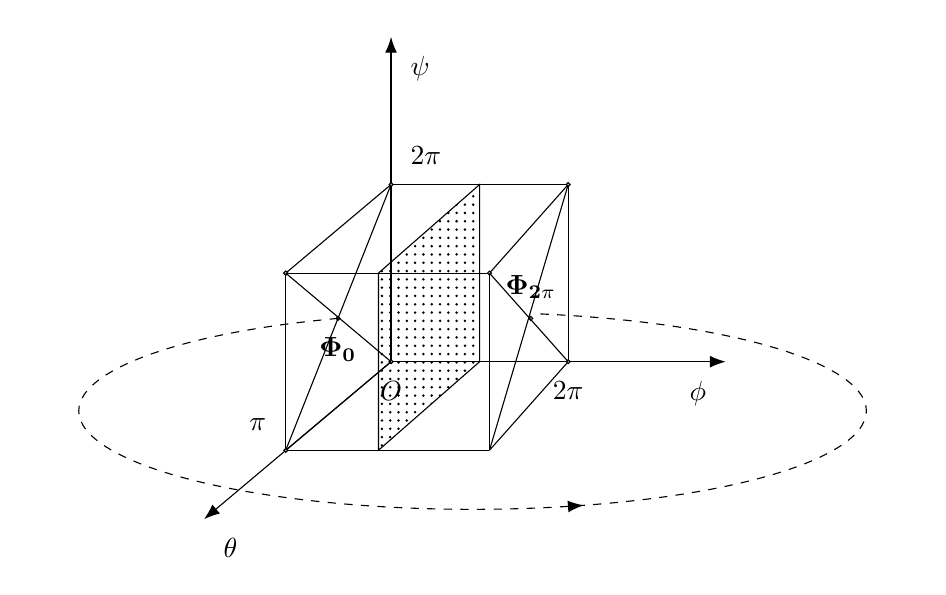
\begin{tikzpicture}[scale=0.25]
\coordinate (O) at (0,0);
\node[label=south :$O$] at (O) {};
\coordinate (X) at (-9.5,-8) {} {};
\coordinate (Y) at (17,0) {} {};
\coordinate (Z) at (0,16.5) {} {};

\coordinate (X0) at (-5.35,-4.5) {} {} ;
\coordinate (Y0) at (9,0) {} ;
\coordinate (Z0) at (0,9) {} {} {} ;
\coordinate (XY) at (5,-4.5) {} {} {} ;
\coordinate (YZ) at (9,9) {} {} ;
\coordinate (XZ) at (-5.35,4.5) {} {};
\coordinate (XYZ) at (5,4.5) {} {} {};


\coordinate (HXY1) at (-0.64,-4.5) {} {} {};
\coordinate (HXY2) at (-0.64,4.5) {} {} {};
\coordinate (HZY1) at (4.5,9) {} {} {};
\coordinate (HZY2) at (4.5,0) {} {} {};


\draw [-{Latex[length=2mm]}] (O) -- (X);
\draw [-{Latex[length=2mm]}] (O) -- (Y);
\draw [-{Latex[length=2mm]}] (O) -- (Z);
\node[label=south east:$\theta$] at (X) {};
\node[label=south west:$\phi$] at (Y) {};
\node[label=south east:$\psi$] at (Z) {};
\node[label=north west:$\pi$] at (X0) {};
\node[label=south :$2\pi$] at (Y0) {};
\node[label=north east:$2\pi$] at (Z0) {};
%\node (Sb) [rectangle, minimum width=3cm, minimum height=1cm,draw=black, pattern color=black, pattern = north east lines]{} ;

\draw [] (X0) -- (XY);
\draw [] (Y0) -- (YZ);
\draw [] (Z0) -- (XZ);
\draw [] (X0) -- (XZ);
\draw [] (Y0) -- (XY);
\draw [] (XY) -- (XYZ);
\draw [] (XZ) -- (XYZ);
\draw [] (YZ) -- (XYZ);
\draw [] (YZ) -- (Z0);
\draw [] (O) -- (Z0);
\draw [] (O) -- (X0);
\draw [] (O) -- (Y0);

\draw[fill=white]  (X0) circle (0.1);
\draw[fill=white]  (Y0) circle (0.1);
\draw[fill=white]  (Z0) circle (0.1);

\draw[fill=white]  (XZ) circle (0.1);
\draw[fill=white]  (YZ) circle (0.1);
\draw[fill=white]  (XZ) circle (0.1);
\draw[fill=white]  (O) circle (0.1);
\draw[fill=white]  (XYZ) circle (0.1);

%\draw[pattern color=black, pattern = dots]  (O) rectangle (YZ) node (v0) {};
%\draw[pattern color=black, pattern = dots]  (X0) rectangle (XYZ) node (v1) {};
\coordinate (plane0) at (7.1,2.2) {};
\coordinate (plane1) at (-2.7,2.2) {};
\draw[fill=white]  (plane1) circle (0.1);
\draw[fill=white]  (plane0) circle (0.1);
%\draw[ decoration={markings, mark=at position 0.75 with {\arrow[scale = 1.]{Latex[length=3mm,reversed]}}},    postaction={decorate}](plane0) .. controls (29.5,-2) and (-28,-4) .. (plane1);
\draw[pattern color=black, pattern = dots]  (HXY1) node (v2) {} -- (HXY2) -- (HZY1) -- (HZY2) -- (HZY2) -- cycle;
\draw  (YZ) edge (XY);
\draw  (XYZ) edge (Y0);
\draw  (XZ) edge (O);
\draw  (Z0) edge (X0);
\node[label=north:$\mathbf{\Phi_{2\pi}}$] at (plane0) {};
\node[label=south:$\mathbf{\Phi_{0}}$] at (plane1) {};
\draw [ dashed,decoration={markings, mark=at position 0.55 with {\arrow[scale = 1.]{Latex[length=2mm]}}},    postaction={decorate}](plane1) arc(-70:261:-20cm and -5cm);
\end{tikzpicture}}
	\
    \subfloat[]{
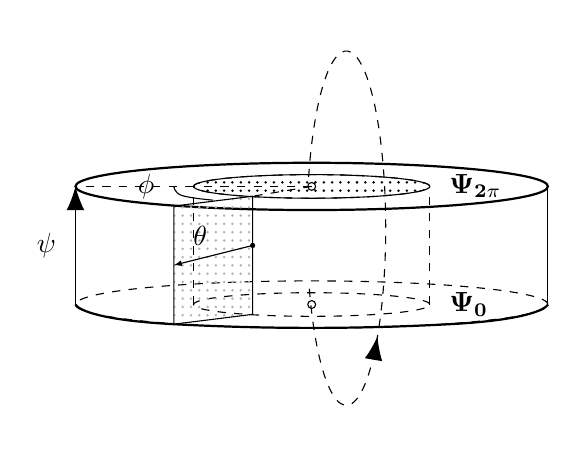
\begin{tikzpicture}[scale=0.5]
\coordinate (O1) at (0,0);
\draw [thick] (O1) ellipse (6 and 0.6);
\coordinate (O2) at (0,-3);
\draw[dashed]  (O2) ellipse (6 and 0.6);
\coordinate (Om) at (0,-1.5);
\coordinate (O1s) at (0,0);
\draw[dashed]  (O1s) ellipse (3 and 0.3);
\coordinate (O2s) at (0,-3);
\draw[dashed]  (O2s) ellipse (3 and 0.3);
\coordinate (Oms) at (0,-1.5);
\draw[pattern color=black, pattern = dots]  (O1) ellipse (3 and 0.3);

%\draw  (O1) ellipse (1 and 0.1);
%\draw[dashed]  (O2) ellipse (1 and 0.1);
\coordinate (Plu) at (-6,0);
\coordinate (Pru) at (6,0);
\coordinate (Pld) at (-6,-3);
\coordinate (Prd) at (6,-3);
\coordinate (Plm) at (-6,-1.5);
\coordinate (Prm) at (6,-1.5);
\coordinate (Plds) at (-3,-3);
\coordinate (Prds) at (3,-3);
\coordinate (Plus) at (-3,0);
\coordinate (Prus) at (3,-0);

\coordinate (Qlu) at (-1,0);
\coordinate (Qru) at (1,0);
\coordinate (Qld) at (-1,-3);
\coordinate (Qrd) at (1,-3);
\draw [-{Latex[length=3mm]}] (Pld) -- (Plu);
\draw [] (Pru) -- (Prd);
\draw [dashed] (Plds) -- (Plus);
\draw [dashed] (Prds) -- (Prus);
%\draw [dashed] (Qlu) -- (Qld);
%\draw [dashed] (Qru) -- (Qrd);
\coordinate (Pu0) at (-1.5,-0.25) {};
\coordinate (Pd0) at (-1.5,-3.25) {};
\coordinate (Pu) at (-3.5,-0.5) {};
\coordinate (Pdl) at (-3.5,-3.5) {} {};
\coordinate (Pdr) at (3.5,-3.5) {} {};
\coordinate (Pmu) at (-3.5,-2) {} {};
\coordinate (Pml) at (-1.5,-1.5) {} {};
\draw[thick]  plot[ smooth,tension=.9] coordinates {(Pld) (Pdl) (Pdr) (Prd)};
\draw [dashed] (Plus) -- (Plu);
\draw[pattern color=gray!60, pattern = dots]  (Pu0) node (v2) {} -- (Pu) -- (Pdl) -- (Pd0) -- (Pu0) -- cycle;
\node[label=west:$\mathbf{\psi}$] at (Plm) {};
\node[label=north east :$\theta$] at (Pmu) {};
\draw  plot[ smooth,tension=.7] coordinates {(-3.5,0) (-3.3,-0.23) (-2.5,-0.35)};
\node[label=west :$\mathbf{\phi}$] at (-3.5,0) {};
\draw [-{Latex[length=1mm]}] (Pml) -- (Pmu);
\draw[fill=white]  (O1) circle (0.1);
\draw[fill=white]  (O2) circle (0.1);
%\draw[ decoration={markings, mark=at position 0.7 with {\arrow[scale = 1.5]{Latex[length=3mm,reversed]}}},    postaction={decorate}](O2) .. controls (3.5,-16.5) and (3.5,11) .. (O1);
\node[label=east:$\mathbf{\Psi_{2\pi}}$] at (Prus) {};
\node[label= east:$\mathbf{\Psi_{0}}$] at (Prds) {};
\draw[fill=black]  (Pml) circle (0.051);
\draw [dashed] (O1) -- (Plus);
\draw [dashed] (O1) -- (Pu0);
\coordinate (Om) at (-0.06,-2.6) {};
\draw [ dashed,decoration={markings, mark=at position 0.32 with {\arrow[scale = 1.]{Latex[length=3mm]}}},    postaction={decorate}](Om) arc (20:345:-1 and -4.5);
\end{tikzpicture}}
    \qquad
    \subfloat[]{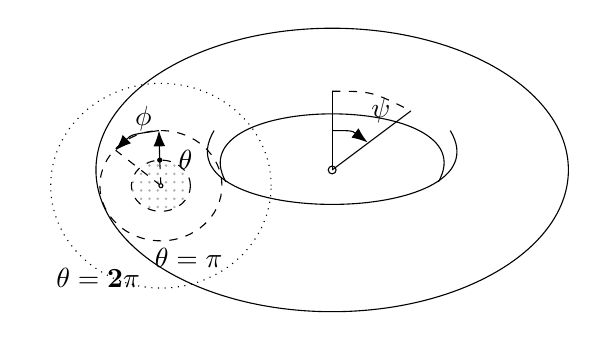
\begin{tikzpicture}[scale=0.5]
\coordinate (O1) at (0,0);
\draw  (O1) ellipse (6 and 3.6);
\coordinate (t1l) at (-3,1.0);
\coordinate (t1r) at (3,1.0);
\coordinate (t1c1) at  (-4.5,-1.5);
\coordinate (t1c2) at (4.5,-1.5);
\draw (t1l) .. controls  (t1c1)  and (t1c2)  .. (t1r);

\coordinate (t2l) at (-2.7,-0.3) {};
\coordinate (t2r) at (2.7,-0.3) {};
\coordinate (t2c1) at (-4,2) {};
\coordinate (t2c2) at (4,2) {};
\draw (t2l) .. controls  (t2c1)  and (t2c2)  .. (t2r);
\draw[fill=white]  (O1) circle (0.1);
\coordinate (a0) at (0,2) {};
\coordinate (a1) at (2,1.5) {} {};
\draw [] (O1) -- (a0);
\draw [] (O1) -- (a1);
\coordinate (ac1) at (1,2) {} {};
\coordinate (ac2) at (1,2) {} {};

\draw [dashed] (a0) .. controls  (ac1)  and (ac2)  .. (a1);
\coordinate (b0) at (0,1.) {};
\coordinate (b1) at (0.9,0.7) {} {};
\coordinate (bc1) at (0.5,1) {} {} {};
\coordinate (bc2) at (0.5,1) {} {} {};
\coordinate (bc3) at (0,0.5) {} {} {} {};
\draw [-{Latex[length=2mm]}]  (b0) .. controls  (bc1)  and (bc2)  .. (b1);
\coordinate (ac3) at (0.5,0.7) {} {} {};
\node[label=north east:$\mathbf{\psi_{}}$] at (ac3) {};
\coordinate (C1) at (-4.35,-.4);
\draw [dashed] (C1) ellipse (1.55 and 1.4);
\draw [dashed,pattern color=gray!60, pattern = dots] (C1) ellipse (0.75 and 0.65);
\draw [dotted] (C1) ellipse (2.8 and 2.6);

\coordinate (C2a) at (-4.38,0.25) {};
\coordinate (C2b) at (-4.4,1) {};
\coordinate (C3b) at (-5.5,0.5) {};
\coordinate (C3a) at (-5,0) {} {};
\draw [dashed] (C1) -- (C2a);
\draw [-{Latex[length=2mm]}] (C2a) -- (C2b);
\draw [dashed] (C1) -- (C3b);
\draw[fill=black]  (C2a) circle (0.051);
%\draw[fill=black]  (C3a) circle (0.051);
\draw[fill=white]  (C1) circle (0.051);
\draw [-{Latex[length=2mm]}] (C2b) .. controls  (-5.1,0.9)  and (-5.1,0.9)  .. (C3b);
\node[label=south east:$\mathbf{\theta}$] at (C2b) {};
\node[label=north east:$\mathbf{\phi}$] at (C3b) {};
\node at (-7,-2.5) {};
\node[label=south east:$\mathbf{\theta = 2\pi}$] at (-7.5,-2) {};
\node at (-3,-1.5) {};
\node[label=south east:$\mathbf{\theta = \pi}$] at (-5,-1.5) {};
\end{tikzpicture}}
\caption{Map of the configuration space of a rigid body with fixed point.}
\label{fig:fig_p181}
\end{figure}
Consider figure $5.2 (a)$. We can stretch like an accordion the cuboid along the $\phi$ axis and bent it so that the planes $\phi=0$ and $\phi=2\pi$ join. We get $(b)$,  a torus with square sections. The dimension $\phi$ is dealt with as a point $P\left( \theta, \phi, \psi \right)$ in the configuration space  returns to the same point when varying $\phi$ to $\phi+2k\pi$.\\
We can apply the same procedure of stretching and bending for the $\psi$ dimension so that the planes $\Psi=0$ and $\Psi=2\pi$ join.
We get $(c)$,  a torus-like object.\\
The only dimension left is $\theta$ which our multi-dimensional crippled mind can't find a way to reshape this pseudo-torus so that when varying $\theta$ we can come back to the same point as started.
$$\blacklozenge$$
\newpage




\section{p183 - Clarification for 5.561}
\begin{tcolorbox}
The kinetic energy is 
$$\mathbf{5.561.}\spatie T=\half I\left(\dot{\theta}^2+\dot{\phi}^2+\dot{\psi}^2+2\dot{\phi}\dot{\psi}\cos{\theta} \right)$$ 
\end{tcolorbox}
We first determine the general form of the kinetic energy for a rigid body rotating around a fixed point.
From $\mathbf{5,310}$ we have
\begin{align}
v_r&= - \omega_{rm}z_m= -\epsilon_{rst}\omega_s z_t\\
T&= \half\sum m v_r v_r\\
\Rightarrow\spatie T&= \half\sum m \epsilon_{rst}\omega_s z_t\epsilon_{ruv}\omega_u z_v\\
&=\half \sum m \left(\delta_{su}\delta_{tv}\omega_s \omega_u z_tz_v - \delta_{sv}\delta_{tu}\omega_s \omega_u z_tz_v  \right)
\end{align}
For the case $N=3$ we get from $(4)$:
\begin{align}
T&= \half\sum m  \left[ \omega_1^2 \left( z_2^2+z_3^2 \right)+\omega_2^2\left( z_1^2+z_3^2 \right)+\omega_3^2 \left( z_1^2+z_2^2 \right)
-2\omega_1 \omega_2 z_1 z_2 -2\omega_1 \omega_3 z_1 z_3 -2\omega_2 \omega_3 z_2 z_3 \right]
\end{align}
Using the result from $\mathbf{5.336}$ this can be written as 
\begin{align}
T&= \half \left[ I_{11}\omega_1^2 +I_{22}\omega_2^2+I_{33}\omega_3^2 
+2I_{12}\omega_1 \omega_2+2I_{13}\omega_1 \omega_3 +2I_{23}\omega_2 \omega_3  \right]
\end{align}
Considering that the matrix $I_{ij}$ is symmetric, one can always find an appropriate basis so that the matrix becomes diagonal. Hence $(6)$ can be simplified to
\begin{align}
T&= \half \left[ I_{11}\omega_1^2 +I_{22}\omega_2^2+I_{33}\omega_3^2 
 \right]
\end{align}
Of course the $\omega_i$ in $(7)$ are not the Euler angles and we have to express the $\omega_i$ as functions of the Euler angles.

\begin{figure}[H]
\begin{center}
\tdplotsetmaincoords{70}{130}
\begin{tikzpicture}[tdplot_main_coords,scale=5]
		%%Styles
		\tikzstyle{init} = [black];			% observers base
		\tikzstyle{prec} = [blue]	;		% second rotation
		\tikzstyle{nuta} = [red]	;		% second rotation
		\tikzstyle{rotp} = [brown];		% thrid rotation
		\tikzstyle{base} = [thick,-Latex]	;% basis
		\tikzstyle{angle} = [thick,-latex]	;%angles
		\tikzstyle{circle} = [thin,dashed]	;%circles
 
		%Parameters	
		\def\epsi{15};	%  precession angle
		\def\etheta{25};	% nutation angle
		\def\ethetatwo{25};	% nutation angle helping
		\def\ephi{15};	% rotation angle
		\def\rang{0.7};	% radius arc angles
 
		%% 
		% observers basis
		\coordinate (O) at (0,0,0);
		\draw[base,init] (O) -- (1.,0,0) node[anchor=north east]{$\overrightarrow{x}$};
		\draw[dashed,thick,init] (O) -- (-1,0,0) node[anchor=north east]{$$};
		\draw[base,init] (O) -- (0,1,0) node[anchor=north east]{$\overrightarrow{y}$};
		\draw[base,init] (O) -- (0,0,1) node[anchor=north west]{$\overrightarrow{z} $};
		\coordinate (Z0) at (0,0,1.4);
		%\draw[tdplot_rotated_coords,blue,, dashed ] (0,-1.2,0) --(0,-1,0) node[anchor=west]{$$};
		\draw[blue,thick, dashed ] (0,0,1) --(Z0) node[anchor=west]{$$};

		
		
		% Precession
		\tdplotsetrotatedcoords{\epsi}{0}{0};
		\draw[tdplot_rotated_coords,angle,prec] (O) --(1,0,0) node[anchor=north west]{$\overrightarrow{u}$};
		\draw[tdplot_rotated_coords,angle,blue,ultra  thick] (O) --(0,1,0) node[anchor=north west,]{$\overrightarrow{N}$};
		\draw[tdplot_rotated_coords,thick,prec,,ultra  thick] (O) --(0,-1,0) node[anchor=west]{$$};
		%\tdplotdrawarc[tdplot_rotated_coords,circle,prec]{(0,0,0)}{1}{0}{360}{}{};
		\tdplotdrawarc[tdplot_rotated_coords,ultra thick,,prec,dashed,-Latex]{(0,0,1.25)}{0.15}{-350}{10}{}{};
		\coordinate (psi) at (0,0.1,1.4);
		\draw[](psi) node[{anchor= west},blue] {$1^{st}\rightarrow \dot{\psi}$};
		%\draw plot [mark=*, mark size=0.10] coordinates{(0,0,0.95)}; 
		\tdplotdrawarc[tdplot_rotated_coords,black,ultra thick]{(0,0,0)}{1}{-90}{90}{}{}	;
		\tdplotdrawarc[tdplot_rotated_coords,dashed,black,ultra thick]{(0,0,0)}{1}{90}{270}{}{}	;		
		\tdplotdrawarc[tdplot_rotated_coords,angle,prec]{(0,0,0)}{\rang}{90-\epsi}{90}{anchor=north east,prec}{$\psi$};	
		\tdplotdrawarc[tdplot_rotated_coords,angle,prec]{(0,0,0)}{\rang}{-\epsi}{0}{anchor=north east,prec}{$\psi$};	
		\draw[tdplot_rotated_coords,red,thick, dashed ] (0,1.4,0) --(0,1,0) node[anchor=west]{$$};
		\draw[tdplot_rotated_coords,red,thick,, dashed ] (0,-1.2,0) --(0,-1,0) node[anchor=west]{$$};
		
		% Nutation
		\tdplotsetrotatedcoords{\epsi}{\ethetatwo}{0};
		\tdplotdrawarc[tdplot_rotated_coords,rotp,ultra thick]{(0,0,0)}{1}{90}{270}{}{};
		\draw[tdplot_rotated_coords,,nuta] (O) --(-1,0,0) node[anchor=north east]{$$};
		\tdplotsetrotatedcoords{\epsi}{\etheta}{0};
		\draw[tdplot_rotated_coords,base,nuta] (O) --(1,0,0) node[anchor=north east]{$\overrightarrow{x}_0$};
		\draw[tdplot_rotated_coords,base,nuta] (O) --(0,0,1) node[anchor=west]{$\overrightarrow{z}_1$};
		\tdplotsetrotatedthetaplanecoords{0};
		\tdplotdrawarc[tdplot_rotated_coords,circle,dashdotted,red]{(0,0,0)}{1}{0}{360}{}{}	;	
		\tdplotdrawarc[tdplot_rotated_coords,angle,nuta]{(0,0,0)}{\rang}{90-\etheta}{90}{anchor=south west,nuta}{$\theta$};		
		\tdplotdrawarc[tdplot_rotated_coords,angle,nuta]{(0,0,0)}{\rang}{-\etheta}{0}{anchor=north,nuta}{$\theta$};
		\tdplotdrawarc[tdplot_rotated_coords,ultra thick,nuta,dashed,-Latex]{(0,0,1.3)}{0.15}{-340}{80}{}{};		
 		\coordinate (theta) at (0,1.6,0.4);
		\draw[](theta) node[{anchor= west},red] {$2^{nd}\rightarrow\dot{\theta}$};
		%\draw plot [mark=*, mark size=0.510] coordinates{(0,0.95,0.2)}; 
		
		
		% Spin
		\tdplotsetrotatedcoords{\epsi}{\etheta}{\ephi};
		\draw[tdplot_rotated_coords,base,rotp] (O) --(1,0,0) node[anchor=north]{$\overrightarrow{x}_1$};
		\draw[tdplot_rotated_coords,base,rotp] (O) --(0,1,0) node[anchor=west]{$\overrightarrow{y}_1$};
		\tdplotdrawarc[tdplot_rotated_coords,ultra thick,dashed,rotp]{(0,0,0)}{1}{-105}{-87}{}{};	
		\tdplotdrawarc[tdplot_rotated_coords,ultra thick,rotp]{(0,0,0)}{1}{-87}{90}{}{};		
		\tdplotdrawarc[tdplot_rotated_coords,angle,rotp]{(0,0,0)}{\rang}{90-\ephi}{90}{anchor=west,rotp}{$\varphi$}	;	
		\tdplotdrawarc[tdplot_rotated_coords,angle,rotp]{(0,0,0)}{\rang}{-\ephi}{0}{anchor=north,rotp}{$\varphi$};	
		\tdplotdrawarc[tdplot_rotated_coords,ultra thick,,rotp,dashed,-Latex]{(0,0,1.43)}{0.15}{0}{360}{}{};		
 		\coordinate (phi) at (0,-0.9,0.9);
		\draw[](phi) node[{anchor=west},rotp] {$3^{rd}\rightarrow\dot{\varphi}$};
		\draw[tdplot_rotated_coords,brown,thick,, dashed ] (0,0,1) --(0,0,1.64) node[anchor=west]{$$};
		% Base
		\tdplotsetrotatedcoords{0}{0}{0};
		\draw[tdplot_rotated_coords,gray,  fill=white,,thick](0,0,0) circle[radius=0.4pt];
		\draw[tdplot_rotated_coords,gray,  fill=white,,thick](0,0,1.25) circle[radius=0.4pt];
		% Precession
		\tdplotsetrotatedcoords{\epsi}{0}{0};
		\draw[tdplot_rotated_coords,gray,  fill=white,,thick](0,-1,0) circle[radius=0.4pt];
		\draw[tdplot_rotated_coords,gray,  fill=white,,thick](0,1,0) circle[radius=0.4pt];
		\draw[tdplot_rotated_coords,gray,  fill=white,,thick](0,1.3,0) circle[radius=0.4pt];
		% Nutation
		\tdplotsetrotatedcoords{\epsi}{\ethetatwo}{0};
		\draw[tdplot_rotated_coords,gray, fill=white, thick](-1,0,0) circle[radius=0.4pt];
		\draw[tdplot_rotated_coords,gray, fill=white, thick](0,0,1.430) circle[radius=0.4pt];
		\end{tikzpicture};
\caption{Euler angles}
\label{fig:fig_p183_5.561}
\end{center}
\end{figure}

Consider the Euler angles as in figure 5.5. The resulting angular velocity of the rigid body can be expressed as 
\begin{align}
\overline{\omega}&= \dot{\psi}\overline{z}+\dot{\theta}\overline{N}+\dot{\phi}\overline{z}_1
\end{align}
The projection of $\overline{\omega}$ on the basis $\overline{x}_1,\overline{y}_1,\overline{z}_1$ (which we choose fixed to the rigid body) will then coincide with the $\omega_i$.\\
We determine the components of $\overline{z},\overline{N},\overline{z}_1$ with $\overline{x}_1,\overline{y}_1,\overline{z}_1$ as basis.\\
We have
\begin{align}
& \left\{\begin{array}{l}
\overline{N}=\cos{\phi} \ \overline{y}_1+\sin{\phi} \ \overline{x}_1\\
\overline{z}= \cos{\theta} \ \overline{z}_1-\sin{\theta}\ \overline{x}_0\\
\overline{x}_0=\cos{\phi} \ \overline{x}_1-\sin{\phi} \ \overline{y}_1
\end{array}\right.\\
\Rightarrow \spatie &\left\{\begin{array}{l}
\overline{N}=\cos{\phi} \ \overline{y}_1+\sin{\phi} \ \overline{x}_1\\
\overline{z}= \cos{\theta} \ \overline{z}_1-\sin{\theta}\ \cos{\phi} \ \overline{x}_1 +\sin{\theta}\ \sin{\phi} \ \overline{y}_1
\end{array}\right.
\end{align}
Hence,
\begin{align}
 \overline{\omega}&= \dot{\psi}\cos{\theta} \ \overline{z}_1-\dot{\psi}\sin{\theta}\ \cos{\phi} \ \overline{x}_1 +\dot{\psi}\sin{\theta}\ \sin{\phi} \ \overline{y}_1+\dot{\theta}\cos{\phi} \ \overline{y}_1+\dot{\theta}\sin{\phi} \ \overline{x}_1+\dot{\phi}\overline{z}_1
\end{align}
giving
\begin{align}
\left\{\begin{array}{l}
\omega_1= \dot{\theta}\sin{\phi} -\dot{\psi}\sin{\theta}\ \cos{\phi}\\
\omega_2= \dot{\psi}\sin{\theta}\ \sin{\phi}+\dot{\theta}\cos{\phi}\\
\omega_3= \dot{\psi}\cos{\theta} +\dot{\phi}\\
\end{array}\right.
\end{align}
In the case  considered $I_{11}=I_{22}=I_{33}=I$. Plugging $(12)$ in $(7)$ gives indeed
$$T=\half I\left(\dot{\theta}^2+\dot{\phi}^2+\dot{\psi}^2+2\dot{\phi}\dot{\psi}\cos{\theta} \right)$$


$$\blacklozenge$$
\newpage

\section{p186 - Exercise 1}
\begin{tcolorbox}
If a vector at the point with coordinates $\left(1,1,1\right)$ in Euclidean $3$-space has components $\left(3,-1,2\right)$, find the contra-variant, covariant and physical components in spherical polar coordinates.
\end{tcolorbox}
The tensor $T_n$ to consider is $\left(3,-1,2\right) - \left(1,1,1\right)= \left(2,-2,1\right)$.\\
The Jacobian matrix for the transformation $z^n \rightarrow x^k$, evaluated at the point $\left(1,1,1\right)$ is 
\begin{align}
J_{\left(1,1,1\right)}&={\begin{pmatrix}{\dfrac {x}{r}}&{\dfrac {y}{r}}&{\dfrac {z}{r}}\\\\{\dfrac {xz}{r^{2}{\sqrt {x^{2}+y^{2}}}}}&{\dfrac {yz}{r^{2}{\sqrt {x^{2}+y^{2}}}}}&{\dfrac {-(x^{2}+y^{2})}{r^{2}{\sqrt {x^{2}+y^{2}}}}}\\\\{\dfrac {-y}{x^{2}+y^{2}}}&{\dfrac {x}{x^{2}+y^{2}}}&0\end{pmatrix}}\\
&=\begin{pmatrix}\dfrac {1}{\sqrt{3}}&\dfrac {1}{\sqrt{3}}&\dfrac {1}{\sqrt{3}}\\\\ \dfrac {1}{3\sqrt{2}}& \dfrac {1}{3\sqrt{2}}&-\dfrac {\sqrt{2}}{3}\\\\ -\dfrac {1}{2}&\dfrac {1}{2}&0\end{pmatrix}\\
\Rightarrow \spatie 
\begin{pmatrix}
r\\
\theta\\
\phi
\end{pmatrix}_{T^{'n}}&=\begin{pmatrix}\dfrac {1}{\sqrt{3}}&\dfrac {1}{\sqrt{3}}&\dfrac {1}{\sqrt{3}}\\\\ \dfrac {1}{3\sqrt{2}}& \dfrac {1}{3\sqrt{2}}&-\dfrac {\sqrt{2}}{3}\\\\ -\dfrac {1}{2}&\dfrac {1}{2}&0\end{pmatrix}\begin{pmatrix}
2\\
-2\\
1
\end{pmatrix}\\
&=\begin{pmatrix}
\dfrac {1}{\sqrt{3}}\\
-\dfrac {\sqrt{2}}{3}\\
-2
\end{pmatrix}
\end{align}
We have the metric tensor evaluated at $\left(1,1,1\right)$
\begin{align}
a_{mn} &= \begin{pmatrix}
1&0&0\\\\
0&r^2&0\\\\
0&0&r^2\sin^2\theta\\\\
\end{pmatrix}=\begin{pmatrix}
1&0&0\\\\
0&3&0\\\\
0&0&2\\\\
\end{pmatrix}\\
\Rightarrow \spatie 
\begin{pmatrix}
r\\
\theta\\
\phi
\end{pmatrix}_{T^{'}_n}&=\begin{pmatrix}
1&0&0\\\\
0&3&0\\\\
0&0&2\\\\
\end{pmatrix}\begin{pmatrix}
\dfrac {1}{\sqrt{3}}\\
-\dfrac {\sqrt{2}}{3}\\
-2
\end{pmatrix}\\
&=\begin{pmatrix}
\dfrac {1}{\sqrt{3}}\\
-\sqrt{2}\\
-4
\end{pmatrix}
\end{align}
And the physical components 
\begin{align}
\begin{pmatrix}
r\\
\theta\\
\phi
\end{pmatrix}_{T^{'}_{ph.}}&=\begin{pmatrix}
1&0&0\\\\
0&\frac{1}{\sqrt{3}}&0\\\\
0&0&\frac{1}{\sqrt{2}}\\\\
\end{pmatrix}\begin{pmatrix}
\dfrac {1}{\sqrt{3}}\\
-\sqrt{2}\\
-4
\end{pmatrix}\\
&=\begin{pmatrix}
\dfrac {1}{\sqrt{3}}\\
-\sqrt{\dfrac {{2}}{{3}}}\\
-2\sqrt{2}
\end{pmatrix}
\end{align}
Another way to find the physical components is to project orthogonally the tensor on the unit vectors of a local Cartesian coordinate system, oriented along the unit vectors $\overline{e}_r,\overline{e}_{\theta},\overline{e}_{\phi}$ corresponding to the vector $P \left(1,1,1\right)$ with modulus $\left|P \right|=\sqrt{3}$. 
We have for the tensor $T_n (2,-2,1)$ with modulus $\left|T_n \right|=3$ as component along $\overline{e}_r$:
\begin{align}
\left|T_n \right|\cos \alpha &= \left|T_n \right|\frac{\left<T_n,P  \right>}{\left|T_n \right|\left|P \right|}\\
&= \left|T_n \right|\frac{2-2+1}{\left|T_n \right|\left|P \right|}\\
&= \frac{1}{\sqrt{3}}
\end{align}
For the component along $\overline{e}_{\theta}$ we first have to determine the vector $\overline{e}_{\theta}$. As first equation we have the orthogonality condition with $\overline{e}_r$ and putting $\overline{e}_{\theta} = (a,b,c)$, get $\left<\overline{e}_r,\overline{e}_{\theta}  \right>=  a+b+c=0$. As $\overline{e}_{\theta}$ lies in the plane $(1,1,0)-(0,0,0)-(0,0,1)$ we can put $a=b$ and get $\overline{e}_{\theta} =  \frac{1}{\sqrt{6}}\left(1,1,-2\right)$ and get for the tensor $T_n (2,-2,1)$  as component along $\overline{e}_{\theta}$:
\begin{align}
\left|T_n \right|\cos \beta &= \left|T_n \right|\frac{\left<T_n,\overline{e}_{\theta}  \right>}{\left|T_n \right|}\\
&= \left|T_n \right|\frac{2-2-2}{\left|T_n \right|\sqrt{6}}\\
&= -\frac{\sqrt{2}}{\sqrt{3}}
\end{align}
For the component along $\overline{e}_{\phi}$ we first have to determine the vector $\overline{e}_{\phi}$. As first equation we have the orthogonality condition with the pair $\overline{e}_r,\overline{e}_{\theta}$  and  get $\overline{e}_{\phi} = \overline{e}_r \times \overline{e}_{\theta}  =  \frac{1}{\sqrt{3}\sqrt{6}}\left( -3,3,0\right)= \left( -\frac{1}{\sqrt{2}},\frac{1}{\sqrt{2}},0\right)$.\\
For the tensor $T_n (2,-2,1)$  as component along $\overline{e}_{\phi}$:
\begin{align}
\left|T_n \right|\cos \gamma &= \left|T_n \right|\frac{\left<T_n,\overline{e}_{\phi}  \right>}{\left|T_n \right|}\\
&= \left|T_n \right|\frac{-2-2}{\left|T_n \right|\sqrt{2}}\\
&= -\frac{4}{\sqrt{2}}\\
&= -2\sqrt{2}
\end{align}
giving
\begin{align}
\begin{pmatrix}
r\\
\theta\\
\phi
\end{pmatrix}_{T^{'}_{ph.}}
&=\begin{pmatrix}
\dfrac {1}{\sqrt{3}}\\
-\sqrt{\dfrac {{2}}{{3}}}\\
-2\sqrt{2}
\end{pmatrix}
\end{align}
as in (9).
$$\blacklozenge$$
\newpage



\section{p186 - Exercise 2}
\begin{tcolorbox}
In cylindrical coordinates $\left(r, \phi,z\right)$ in Euclidean $3$-space, a vector field is such that the vector at each point points along the parametric line of $\phi$, in the sense of $\phi$ increasing, and its magnitude is $kr$, where $k$ is a constant. Find the contra-variant, covariant and physical components of this vector field.
\end{tcolorbox}
We can work backwards, with the physical components as starting point. Indeed, at a point $P\left(r,\phi,z\right)$ the tensor of this vector field will have $\left(0,kr,0\right)$ as physical components in the cylindrical coordinates $\left( r, \phi,z \right)$ system.\\
We have the metric tensor 
\begin{align}
a_{mn} &= \begin{pmatrix}
1&0&0\\\\
0&r^2&0\\\\
0&0&1\\\\
\end{pmatrix}
\end{align}
Giving
\begin{align}
\left\{\begin{array}{lll}
X_1 = &h_1 X_{1}^{phys.}&=0\\\\
X_2 = &h_2 X_{2}^{phys.}&=kr^2\\\\
X_3 = &h_3 X_{3}^{phys.}&=0\\\\
\end{array}\right.
\end{align}
and 
\begin{align}
\left\{\begin{array}{lll}
X^1 = &\frac {X_{1}^{phys.}}{h_1}&=0\\\\
X^2 = &\frac {X_{2}^{phys.}}{h_2}&=k\\\\
X^3 = &\frac {X_{3}^{phys.}}{h_3}&=0\\\\
\end{array}\right.
\end{align}

$$\blacklozenge$$
\newpage




\section{p186 - Exercise 3}
\begin{tcolorbox}
Find the physical components of velocity and acceleration along the parametric lines of cylindrical coordinates in terms of the  and their derivatives with respect to time.
\end{tcolorbox}
We have the metric tensor 
\begin{align}
a_{mn} &= \begin{pmatrix}
1&0&0\\\\
0&r^2&0\\\\
0&0&1\\\\
\end{pmatrix}
\end{align}
and the contravariant velocities

\begin{align}
\left\{\begin{array}{lll}
v^1= &\dv{r}{t}\\\\
v^2= &\dv{\phi}{t}\\\\
v^3= &\dv{z}{t}\\\\
\end{array}\right.
\end{align}
giving by $v_{K}^{phys.} = h_K v^K$
\begin{align}
\left\{\begin{array}{lll}
v_r= &\dv{r}{t}\\\\
v_{\phi}= &r\dv{\phi}{t}\\\\
v_z= &\dv{z}{t}\\\\
\end{array}\right.
\end{align}
For the acceleration using $f^r=\fdv{v^r}{t} $
and the Christoffel symbols being 
\begin{align}
\left \{ \begin{array}{c}
\Gamma^m_{nk} = 0 \quad\forall\quad (nk) \ne (r, \theta), (\theta, \theta)\\\\
\Gamma^{\theta}_{r\theta} = \frac{1}{r} \quad\text{and}\quad \Gamma^r_{\theta\theta} = -r
\end{array}\right.\
\end{align}
we have
\begin{align}
\left\{\begin{array}{lll}
f^1= &\dv{v^1}{t}-r\underbrace{v^2\dv{x^2}{t}}_{=\left(v^2\right)^2}\\\\
f^2= &\dv{v^2}{t}+\underbrace{\frac{1}{r}v^1\dv{x^2}{t}+\frac{1}{r}v^2\dv{x^21}{t}}_{=\frac{2}{r}v^1 v^2}\\\\
f^3= &\dv{v^3}{t}\\\\
\end{array}\right.
\end{align}
giving by $f_{K}^{phys.} = h_K f^K$
\begin{align}
&\left\{\begin{array}{lll}
f_r= &\dv{v^1}{t}-r\left(v^2\right)^2\\\\
f_{phi}= &r\dv{v^2}{t}+r\frac{2}{r}v^1 v^2\\\\
f_z= &\dv{v^3}{t}\\\\
\end{array}\right.\\
\Rightarrow \spatie &\left\{\begin{array}{lll}
f_r= &\dv[2]{r}{t}-r\left(\dv{\phi}{t}\right)^2\\\\
f_{phi}= &r\dv[2]{\phi}{t}+2\dv{r}{t} \dv{\phi}{t}\\\\
f_z= &\dv[2]{z}{t}\\\\
\end{array}\right.
\end{align}
$$\blacklozenge$$
\newpage



\section{p186 - Exercise 4}
\begin{tcolorbox}
A particle moves on a sphere under the action of gravity. Find the contra-variant an co-variant components of the force, using colatitude and azimuth, and write down the equation of motion.
\end{tcolorbox}
We determine first the physical components of the force.
\begin{figure}[H]

\begin{tikzpicture}[scale=0.5]
\coordinate (O1) at (0,0);
\draw  (O1) circle (6);
%\draw [thick] (O1) ellipse (6 and 0.6);
\coordinate (Om) at (0.0,-6) ;
%\node at (Om){$P$};
\draw [ decoration={markings, mark=at position 0.32 with {\arrow[scale = 1.]{Latex[length=3mm]}}},    postaction={}](Om) arc (90:-90:3 and -6.0);
\draw [ dashed,decoration={markings, mark=at position 0.32 with {\arrow[scale = 1.]{Latex[length=3mm]}}},    postaction={}](Om) arc (90:-90:-3 and -6.0);
\coordinate (Ohl) at (-5.2,3) {} {} {};
\coordinate (Ohr) at (5.2,3) {} {} {};
%\node at (Oh){$P$};
%\draw[fill=white]  (Ohl) circle (0.1);
%\draw[fill=white]  (Ohr) circle (0.1);
\draw [ decoration={markings, mark=at position 0.32 with {\arrow[scale = 1.]{Latex[length=3mm]}}},    postaction={}](Ohl) arc (-10:190:-5.3 and -0.5);
\draw [dashed ,decoration={markings, mark=at position 0.32 with {\arrow[scale = 1.]{Latex[length=3mm]}}},    postaction={}](Ohl) arc (10:190:-5.3 and 0.5);
\coordinate (NPole) at (0,6) {};
\draw[fill=white]  (NPole) circle (0.1);
\coordinate (SPole) at (0,-6) {};
\draw[dashdotted] (NPole) -- (SPole);
\draw[fill=white]  (SPole) circle (0.1);
\coordinate (P) at (2.7,2.5) {};
\draw[fill=white]  (P) circle (0.1);
\draw[fill=white]  (O1) circle (0.1);
\coordinate (etheta) at (3.5,-1) {};
\coordinate (ephi)  at (7,2.5) {};
\draw [-{Latex[length=2mm]}] (P) -- (etheta);
\draw [-{Latex[length=2mm]}] (P) -- (ephi);
\draw[dashed] (O1) -- (P);
\node[label=east:$\mathbf{\overline{1}_{\theta}}$] at (etheta) {};
\node[label=east:$\mathbf{\overline{1}_\phi}$] at (ephi) {};
\node[label=west:$O$] at (O1) {};
\coordinate (O2) at (-0.10,2);
\node[label=south east:$\theta$] at (O2) {};
\draw [dashed, decoration={markings, mark=at position 0.52 with {\arrow[scale = 1.]{Latex[length=2mm]}}},    postaction={decorate}](O2) arc (90:55:3 and 3.0);
\coordinate (F)  at (2.7,0) {};
\draw [-{Latex[length=2mm]}] (P) -- (F);
\node[label=west:$\mathbf{\overline{F}}$] at (F) {};
\coordinate (D0) at (11,-1) {};
\coordinate (DP) at (15.5,4) {};
\node[label=east:$\mathbf{m}$] at (DP) {};
\coordinate (De) at (20.5,0) {};
\coordinate (DF) at (15.5,-3.5) {};
\coordinate (DA) at (11,8.5) {};
\draw [dashed] (D0) -- (DP);
\draw [dashed] (D0) -- (DA);
\draw [-{Latex[length=2mm]}] (DP) -- (De);
\node[label=east:$\mathbf{\overline{1}_{\theta}}$] at (De) {};
\draw [-{Latex[length=2mm]}] (DP) -- (DF);
\node[label=east:$\mathbf{\overline{F}}$] at (DF) {};
\coordinate (thet) at  (11,3) {};
\draw [dashed, decoration={markings, mark=at position 0.52 with {\arrow[scale = 1.]{Latex[length=2mm]}}},    postaction={decorate}](thet) arc (90:35:3 and 3.0);
\node[label=south east:$\theta$] at (thet) {};
\coordinate (thet2) at (15.5,0.5) {};
\draw [dashed, decoration={markings, mark=at position 0.52 with {\arrow[scale = 1.]{Latex[length=2mm]}}},    postaction={decorate}](thet2) arc (90:30:3 and -3.0);
\node[label=south east:$\frac{\pi}{2}-\theta$] at (thet2) {};
\draw[fill=white]  (DP) circle (0.1);
\end{tikzpicture}

\caption{Physical components of the gravitational force tensor acting on a mass $\mathbf{m}$ on a sphere }
\label{fig:fig_p186_Ex2}
\end{figure}
We note first that the unit vector $\overline{1}_{\phi}$ is perpendicular to the place formed by the vectors  $\overline{1}_{\theta},\overline{F}$ and s the force has no components projected on this vector. The vector $\overline{F}$ is parallel with the axis of reference of the sphere with radius $R$ and so the physical components become
\begin{align}
&\left\{\begin{array}{l}
F_{\phi}^{phys}= 0\\\\
F_{\theta}^{phys}= mg\sin{\theta}\\\\
\end{array}\right.\\
\Rightarrow\spatie &\left\{\begin{array}{ll}
F^{\phi}= 0&F_{\phi}= 0\\\\
F^{\theta}= \frac{1}{R}mg\sin{\theta}&F_{\theta}= R m g\sin{\theta}\\\\
\end{array}\right.
\end{align}
We use equation $\mathbf{5.212.}$
\begin{align}
&\left\{\begin{array}{l}
\dv{}{t}\frac{\partial T}{\partial \dot{x}^s} - \frac{\partial T}{\partial x^s} = F_{s}\\\\
T = \half m a_{pq}\dot{x}^p\dot{x}^q, \ \dot{x}^s=\dv{x^s}{t}\\\\
\end{array}\right.
\end{align}
with for our case
\begin{align}
T = \half m R^2\left(\dot{\theta}^2+ \sin^2 \theta \ \dot{\phi}^2 \right)
\end{align}
and get the set of equation of motion (the second column gives the dimensional analysis as a check for consistency)

\begin{align}
&\left\{\begin{array}{lll}
\frac{\ddot{\phi}}{\dot{\phi}}=  -2\cot\theta \  \dot{\theta}&:&\frac{[T]^{-2}}{[T]^{-1}}\cong [T]^{-1}\\\\
\ddot{\theta} - \left(\dot{\phi}\right)^2\sin\theta \cos\theta= \frac{g}{R}\sin{\theta}&:&[T]^{-2}+\left([T]^{-1}\right)^2 \cong \frac{[L][T]^{-2}}{[L]^{}}\\\
\end{array}\right.
\end{align}
Let's check the special case when $\dot{\phi} = 0$.\\
The first equation can be rewritten and gives of course $\phi=C$ while the second equation becomes $$\ddot{\theta} = \frac{g}{R}\sin{\theta}$$
which is similar to the equation of  the simple gravity pendulum.
$$\blacklozenge$$
\newpage

\section{p186 - Exercise 5}
\begin{tcolorbox}
Consider the motion of a particle on a smooth torus under no forces except normal reaction. The geometrical line element may be written $$ ds^2=\left(a-b\cos \theta \right)^2 d{\phi}^2+b^2 d\theta^2$$ where $\phi$ is an azimuthal angle and $\theta$ an angular displacement from the equatorial plane. Show that  the path of a particle satisfies the following two differential equations in which $h$ is a constant 
$$(a)\spatie \left(a-b\cos\theta\right)^2\dv{\phi}{s} = h$$
$$(b)\spatie b^2\left(\dv{\theta}{\phi}\right)^2= \frac{\left(a-b\cos\theta\right)^4}{h^2}-\left(a-b\cos\theta\right)^2$$
\end{tcolorbox}
We use equation $\mathbf{5.212.}$ and  $\mathbf{5.212.}$
\begin{align}
&\left\{\begin{array}{l}
\dv{}{t}\frac{\partial T}{\partial \dot{x}^s} - \frac{\partial T}{\partial x^s} = F_{s}\\\\
T = \half m a_{pq}\dot{x}^p\dot{x}^q, \ \dot{x}^s=\dv{x^s}{t}\\\\
\end{array}\right.
\end{align}
with for our case
\begin{align}
T = \half m \left(b^2\dot{\theta}^2+ \left(a-b\cos \theta \right)^2  \ \dot{\phi}^2 \right)
\end{align}
\begin{align}
&\left\{\begin{array}{ll}
\frac{\partial T}{\partial \dot{\phi}}= m \left(a-b\cos \theta \right)^2   \dot{\phi}&\frac{\partial T}{\partial {\phi}}= 0\\\\
\frac{\partial T}{\partial \dot{\theta}}=  mb^2\dot{\theta}&\frac{\partial T}{\partial {\theta}}=  mb\left(a-b\cos \theta \right)\dot{\phi}^2\sin \theta\\\\
\end{array}\right.
\end{align}giving
\begin{align} 
&\left\{\begin{array}{l}
\left(a-b\cos \theta \right)^2   \ddot{\phi}+2b\left(a-b\cos \theta \right)\dot{\theta} \dot{\phi}\sin \theta  =0\\\\
b^2\ddot{\theta}-b\left(a-b\cos \theta \right)\dot{\phi}^2\sin \theta=0\\\\
\end{array}\right.\\
\Rightarrow\spatie &\left\{\begin{array}{l}
\left(a-b\cos \theta \right)   \ddot{\phi}=-2b\dot{\theta} \dot{\phi}\sin \theta  \\\\
b^2\ddot{\theta}-b\left(a-b\cos \theta \right)\dot{\phi}^2\sin \theta=0\\\\
\end{array}\right.
\end{align}
In the first equation, put $y \equiv \dot{\phi}$ giving for the first equation:
\begin{align}
\frac{dy}{y}&=-2b \frac{\sin \theta d\theta} {\left(a-b\cos \theta \right)}  \\
\Leftrightarrow\spatie\frac{dy}{y}&=-2 \frac{d\left(a-b\cos \theta \right)} {\left(a-b\cos \theta \right)}\\
\Rightarrow \spatie \log y&=-2 \log \left(a-b\cos \theta \right)+\log C^{}\\
\Rightarrow \spatie \dot{\phi}&= C \left(a-b\cos \theta \right)^{-2}
\end{align}
Note that $\dot{\phi}$ is a time derivative. But as we are on a geodesic, $\mathbf{5.226.}$ stands and so $v$ is constant as $\dv{v}{s} =0$. Using $v = \dv{s}{t}$, (9) can be written as 
\begin{align}
\left(a-b\cos \theta \right)^{2}\dv{\phi}{t}&= C \\
\Leftrightarrow\spatie\left(a-b\cos \theta \right)^{2}\dv{\phi}{s}\underbrace{\dv{s}{t}}_{=v}&= C \\
\Leftrightarrow\spatie\left(a-b\cos \theta \right)^{2}\dv{\phi}{s}&= h \quad \text{with } h=\frac{C}{v}
\end{align}
Next, we don't use the second equation in (5) but the line element equation instead
\begin{align}
ds^2&=\left(a-b\cos \theta \right)^2 d{\phi}^2+b^2 d\theta^2\\
\Rightarrow\spatie \left(\dv{s}{\phi}\right)^2 &= \left(a-b\cos \theta \right)^2 +b^2 \left(\dv{\theta}{\phi}\right)^2\\
\Rightarrow\spatie b^2 \left(\dv{\theta}{\phi}\right)^2 &= \left(\dv{\phi}{s}\right)^{-2 }- \left(a-b\cos \theta \right)^2 \\
\left(12\right)\quad \text{: }\spatie b^2 \left(\dv{\theta}{\phi}\right)^2 &= \frac{\left(a-b\cos \theta \right)^4}{h^2}- \left(a-b\cos \theta \right)^2
\end{align}
$$\blacklozenge$$
\newpage



\section{p186 - Exercise 6}
\begin{tcolorbox}
Consider the motion of a particle under gravity on the smooth torus o the previous problem, the equatorial plane of the torus being horizontal. Taking the mass of the particle to unity, so that $V= bg\sin{\theta}$, show that the path of the particle satisfies the following two differential equations. 
$$(a)\spatie \left(E-V\right)\left(a-b\cos\theta\right)^2\dv{\phi}{s} = h$$
$$(b)\spatie b^2\left(\dv{\theta}{\phi}\right)^2=  \left(E-V\right)\frac{\left(a-b\cos\theta\right)^4}{h^2}-\left(a-b\cos\theta\right)^2$$
where $E$ is the total energy,  $h$ is a constant and $d\sigma$ is the action line element.
\end{tcolorbox}
The line of reasoning is quite the same as problem $(5)$.
We use equation $\mathbf{5.212.}$ and  $\mathbf{5.212.}$
\begin{align}
&\left\{\begin{array}{l}
\dv{}{t}\frac{\partial T}{\partial \dot{x}^s} - \frac{\partial T}{\partial x^s} = F_{s}\\\\
T = \half m a_{pq}\dot{x}^p\dot{x}^q, \ \dot{x}^s=\dv{x^s}{t}\\\\
\end{array}\right.
\end{align}
with for our case
\begin{align}
T = \half m \left(b^2\dot{\theta}^2+ \left(a-b\cos \theta \right)^2  \ \dot{\phi}^2 \right)
\end{align}
\begin{align}
&\left\{\begin{array}{ll}
\frac{\partial T}{\partial \dot{\phi}}= m \left(a-b\cos \theta \right)^2   \dot{\phi}&\frac{\partial T}{\partial {\phi}}= 0\\\\
\frac{\partial T}{\partial \dot{\theta}}=  mb^2\dot{\theta}&\frac{\partial T}{\partial {\theta}}=  mb\left(a-b\cos \theta \right)\dot{\phi}^2\sin \theta\\\\
\end{array}\right.
\end{align}giving (as $F_{\phi} = -\partial_{\phi} V = 0$ and $F_{\theta} = -\partial_{\theta} V = -bg\cos{\theta}$)
\begin{align} 
&\left\{\begin{array}{l}
\left(a-b\cos \theta \right)^2   \ddot{\phi}+2b\left(a-b\cos \theta \right)\dot{\theta} \dot{\phi}\sin \theta  =0\\\\
b^2\ddot{\theta}-b\left(a-b\cos \theta \right)\dot{\phi}^2\sin \theta=-bg\cos{\theta}\\\\
\end{array}\right.\\
\Rightarrow\spatie &\left\{\begin{array}{l}
\left(a-b\cos \theta \right)   \ddot{\phi}=-2b\dot{\theta} \dot{\phi}\sin \theta  \\\\
b^2\ddot{\theta}-b\left(a-b\cos \theta \right)\dot{\phi}^2\sin \theta=-bg\cos{\theta}\\\\
\end{array}\right.
\end{align}
In the first equation, put $y \equiv \dot{\phi}$ giving for the first equation:
\begin{align}
\frac{dy}{y}&=-2b \frac{\sin \theta d\theta} {\left(a-b\cos \theta \right)}  \\
\Leftrightarrow\spatie\frac{dy}{y}&=-2 \frac{d\left(a-b\cos \theta \right)} {\left(a-b\cos \theta \right)}\\
\Rightarrow \spatie \log y&=-2 \log \left(a-b\cos \theta \right)+\log C^{}\\
\Rightarrow \spatie \dot{\phi}&= C \left(a-b\cos \theta \right)^{-2}
\end{align}
Note that $\dot{\phi}$ is a time derivative. Using  $\dv{s}{t}=v = \sqrt{2T} = \sqrt{2}\sqrt{E-V}$, (9) can be written as 
\begin{align}
\left(a-b\cos \theta \right)^{2}\dv{\phi}{t}&= C \\
\Leftrightarrow\spatie\left(a-b\cos \theta \right)^{2}\dv{\phi}{\sigma}\underbrace{\dv{\sigma}{s}}_{= \sqrt{E-V}}\underbrace{\dv{s}{t}}_{=\sqrt{2}\sqrt{E-V}}&= C \\
\Leftrightarrow\spatie \left(E-V\right)\left(a-b\cos \theta \right)^{2}\dv{\phi}{\sigma}(E-V)&= h
\end{align}
with $h=\frac{C}{\sqrt{2}}$.\\
Next, we don't use the second equation in (5) but the line element equation instead
\begin{align}
ds^2&=\left(a-b\cos \theta \right)^2 d{\phi}^2+b^2 d\theta^2\\
\Rightarrow\spatie \left(\dv{s}{\phi}\right)^2 &= \left(a-b\cos \theta \right)^2 +b^2 \left(\dv{\theta}{\phi}\right)^2\\
\Rightarrow\spatie b^2 \left(\dv{\theta}{\phi}\right)^2 &= \left(\dv{\phi}{s}\right)^{-2 }- \left(a-b\cos \theta \right)^2 \\
\Leftrightarrow\spatie b^2 \left(\dv{\theta}{\phi}\right)^2 &= \left(\dv{\phi}{\sigma}\right)^{-2 }\left(\dv{\sigma}{s}\right)^{-2 }- \left(a-b\cos \theta \right)^2 \\
\left(12\right)\quad \text{: }\spatie b^2 \left(\dv{\theta}{\phi}\right)^2 &= \left( E-V \right)^2\frac{1}{\left(E-V\right)}\frac{\left(a-b\cos \theta \right)^4}{h^2}- \left(a-b\cos \theta \right)^2\\
\Rightarrow\spatie b^2 \left(\dv{\theta}{\phi}\right)^2 &= \left( E-V \right)\frac{\left(a-b\cos \theta \right)^4}{h^2}- \left(a-b\cos \theta \right)^2
\end{align}
$$\blacklozenge$$
\newpage



\section{p187 - Exercise 7}
\begin{tcolorbox}
A dynamical system consists of a thin straight smooth tube which can rotate in a horizontal plan about one end $O$, together with a bead$B$ inside the tube connected to $O$ by a spring. Taking as coordinates $r=OB$ and $\theta = $ angle of rotation of the tube about $O$, the potential energy $V$ is a function of $r$ only. Show that in configuration space , all the lines of force are geodesics for the kinematical line element.
\end{tcolorbox}
Well understanding the question is of course paramount:
\begin{itemize}
  \item  The tube mentioned plays only a functional role to hold the spring "stiff" along the line $OB$ as its mass can be neglected.It  will play  no further role in the dynamics of the system. 
  \item Nothing is said that the system contains any force that keeps the angular velocity at a constant speed $\omega$. 
\end{itemize}  
That being clarified, one can expect that the system will behave as a harmonic oscillator along the line  $OB$ and that ,given an initial rotational momentum, the angular momentum will be a constant during the trajectory of the bead.
This means that the bead will oscillate along $OB$ but as the angular momentum is a constant and  given $m \omega r^2 =C$($m$ = mass of the bead), the  instant radial speed will vary.\\
The only conservative force acting on the bead will be that of the spring and will be $V=\half k \left( r-r_0 \right)^2$, $r_0$ being the point along $OB$ where the spring is not stretched. The generalized forces are $F_r = - k\left( r-r_0 \right)$ and $F_{\theta}= 0$ meaning the lines of force are straight lines pointing to the origin $O$.\\
About the geodesics. Clearly the instantaneous velocity of the bead is $\overrightarrow{v} = \dot{r}\overrightarrow{1}_r+ \dot{\theta}r\overrightarrow{1}_{\theta}$ giving as kinetic energy $T=\half\left(\dot{r}^2+\dot{\theta}^2 r^2\right)$ giving as kinematic line element
$$ds^2= 2Tdt = dr^2+r^2d\theta^2$$
Referring to $\mathbf{3.101}$, the configuration space is flat and the geodesics are straight lines. As the line forces are straight lines towards the origin $O$, these line of force are also geodesics in the configuration space equipped with the kinematical line element.

$$\blacklozenge$$
\newpage


\section{p187 - Exercise 8}
\begin{tcolorbox}
Show that if a line of force is a geodesic for the kinematical line element, it is also a geodesic for the action line element.
\end{tcolorbox}
From $\mathbf{5.516}$ and  $\mathbf{5.529}$ we have
\begin{align}
X^r = v\dv{v}{s}\lambda^r +\kappa v^2\nu^r
\end{align}
As the line of force is a geodesic, we can start with a velocity tangent to the line of force, ensuring that the trajectory of the dynamical system will lie on the geodesic line of force (see page 175) and thus $\kappa=0$ for the trajectory. Hence,
\begin{align}
X^r = v\dv{v}{s}\lambda^r
\end{align}
expressing now the function of the action line element $d \sigma = \sqrt{E-V}ds $ we have 
\begin{align}
X^r &= v\dv{v}{s}\lambda^r\\
&= v\dv{v}{s}\dv{x^r}{\sigma}\dv{\sigma}{s}\\
&= v\dv{v}{s}\dv{x^r}{\sigma}\sqrt{E-V}\\
&= \sqrt{E-V}v\dv{v}{s}\lambda^{'r}
\end{align}
As stated page 177, this dynamical system will describe in configuration space a geodesic for the action metric, meaning that $\lambda^{'r}$ is tangent to this geodesic and that $X^r$, being collinear with $\lambda^{'r}$ (with the factor $\sqrt{E-V}v\dv{v}{s}$), is also tangent to this geodesic. Hence, this  line of force is also a geodesic for the action line element.
$$\blacklozenge$$
\newpage

\section{p187 - Exercise 9}
\begin{tcolorbox}
Using the methods of Chapter II and $\mathbf{5.532}$, show that the trajectories of a dynamical system with kinetic energy $T$ and potential energy $V$ satisfy the variational equation $$\delta \int_{t_1}^{t_2}\left(T-V\right)dt = 0$$
\end{tcolorbox}
Let's start with a function $L$ defined by 
\begin{align}
dL=(T-V)du\\
\end{align}
As in figure $2$ page 38 we will make $L$ a function of two parameters, $u$ and $v$ , the latter defining a family of curves between the begin  point $u_1$ and the endpoint $u_2$.
\begin{align}
L&= L(u,v)
\end{align}
with 
\begin{align}
(T-V)(u_1,v)=(T-V)_1 \quad (T-V)(u_2,v)=(T-V)_2 \quad \forall v  
\end{align}
We will try to minimize (with respect to $v$) the following functional
\begin{align}
L &= = \int_{u_1}^{u_2}(T-V)(u,v)du
\end{align}
It's derivative with respect to $v$
\begin{align}
\dv{L}{v} &= \int_{u_1}^{u_2}\frac{\partial (T-V)(u,v)}{\partial v}du
\end{align}
We express $(T-V)(u,v)$ as a function of the generalized coordinates $x^r$ and their derivatives. Then,
\begin{align}
\frac{\partial (T-V)(u,v)}{\partial v}&= \frac{\partial (T-V)(u,v)}{\partial \dot{x^r}}\frac{\partial \dot{x^r}}{\partial v}+\frac{\partial (T-V)(u,v)}{\partial x^r}\frac{\partial x^r}{\partial v}
\end{align}
where $\dot{x^r}= \frac{\partial x^r}{\partial u}$.\\
We have 
\begin{align}
\frac{\partial \dot{x^r}}{\partial v} &= \frac{\partial}{\partial v} \frac{\partial x^r}{\partial u}= \frac{\partial}{ \partial u} \frac{\partial x^r}{\partial v}
\end{align}
So, 
\begin{align}
\frac{\partial (T-V)(u,v)}{\partial v}&= \frac{\partial (T-V)(u,v)}{\partial \dot{x^r}}\frac{\partial}{ \partial u} \frac{\partial x^r}{\partial v}+\frac{\partial (T-V)(u,v)}{\partial x^r}\frac{\partial x^r}{\partial v}
\end{align}
Consider the expression
\begin{align}
\int_{u_1}^{u_2}d(AB) &= \int_{u_1}^{u_2}Ad(B) + \int_{u_1}^{u_2}Bd(A)\\
\Rightarrow \spatie \int_{u_1}^{u_2}Ad(B)&=\int_{u_1}^{u_2}d(AB) -\int_{u_1}^{u_2}Bd(A)
\end{align}
Put $B= \frac{\partial x^r}{\partial v}$ and $A=  \frac{\partial (T-V)(u,v)}{\partial \dot{x^r}}$ and putting this inside (9) and (6):
\begin{align}
\dv{L}{v} &= \int_{u_1}^{u_2}d\left(\frac{\partial (T-V)(u,v)}{\partial \dot{x^r}}\frac{\partial x^r}{\partial v} \right)-\int_{u_1}^{u_2}\frac{\partial x^r}{\partial v} d \left(\frac{ \partial (T-V)(u,v)}{\partial \dot{x^r}} \right)+\int_{u_1}^{u_2}\frac{\partial (T-V)(u,v)}{\partial x^r}\frac{\partial x^r}{\partial v}du\\
&=\left.\frac{\partial (T-V)(u,v)}{\partial \dot{x^r}}\frac{\partial x^r}{\partial v} \right|_{u_1}^{u_2}-\left[\int_{u_1}^{u_2}\left(\frac{\partial}{\partial u} \left(\frac{ \partial (T-V)(u,v)}{\partial \dot{x^r}} \right)-\frac{\partial (T-V)(u,v)}{\partial x^r}\right)\frac{\partial x^r}{\partial v} du \right]
\end{align}
We express now the results in term of infinitesimals. A change in "length" $\delta L$ when we pas from a curve $v$ to a curve $v+dv$ is
\begin{align}
\delta L &= \dv{L}{v}\delta v\\
&= \left.\frac{\partial (T-V)(u,v)}{\partial \dot{x^r}}\frac{\partial x^r}{\partial v} \delta v\right|_{u_1}^{u_2}-\int_{u_1}^{u_2}\left(\frac{\partial}{\partial u} \left(\frac{ \partial (T-V)(u,v)}{\partial \dot{x^r}} \right)-\frac{\partial (T-V)(u,v)}{\partial x^r}\right)\frac{\partial x^r}{\partial v}\delta v du\\
&= \left.\frac{\partial (T-V)(u,v)}{\partial \dot{x^r}}\delta x^r\right|_{u_1}^{u_2}-\int_{u_1}^{u_2}\left(\frac{\partial}{\partial u} \left(\frac{ \partial (T-V)(u,v)}{\partial \dot{x^r}} \right)-\frac{\partial (T-V)(u,v)}{\partial x^r}\right)\delta x^r du
\end{align}
The first term vanish as at the endpoints  the $\delta x^r$ are zero and hence we get
\begin{align}
\delta L &= -\int_{u_1}^{u_2}\left(\frac{\partial}{\partial u} \left(\frac{ \partial (T-V)(u,v)}{\partial \dot{x^r}} \right)-\frac{\partial (T-V)(u,v)}{\partial x^r}\right)\delta x^r du
\end{align}
As the $\delta x^r$ are arbitrary, we must have for $\delta L =0$
\begin{align}
\frac{\partial}{\partial u} \left(\frac{ \partial (T-V)(u)}{\partial \dot{x^r}} \right)-\frac{\partial (T-V)(u)}{\partial x^r}&=0
\end{align}
This is the same equation as $\mathbf{5.532}$ which describe the motion of a system with a conservative force. 
$$\blacklozenge$$
\newpage

\section{p188 - Exercise 10}
\begin{tcolorbox}
Using the definition $\mathbf{5.5335}$ for $I_{rs}$, prove that if $X_r$ is any non-zero vector, then $I_{rs}X_rX_s \geq 0$, and that the equality occurs only if all particles of the system are distributed on a single line.
\end{tcolorbox}
By  $\mathbf{5.335}$
\begin{align}
I_{rs}&= \delta_{rs}\sum m z_qz_q - \sum m z_r z_s
\end{align}
Multiplying by $X_rX_s$:

\begin{align}
I_{rs}X_rX_s&= \underbrace{X_r X_s \delta_{rs}}_{=X_rX_r}\sum m z_qz_q - \sum m \underbrace{z_rX_r}_{=\left|z\right|_{(m)}\left|X\right|\cos{\theta}_m }\underbrace{ z_sX_s}_{=\left|z\right|_{(m)}\left|X\right|\cos{\theta}_m }
\end{align}
with $\theta_m$ the angle between the vector $X_r$ and the position vector $z_m$ of a particle.
\begin{align}
I_{rs}X_rX_s &=\left|X\right|^2\sum m \left|z\right|_{(m)}^2 - \left|X\right|^2\sum m\left|z\right|_{(m)}^2\cos^2{\theta}_m \\
&=\left|X\right|^2\sum m \left|z\right|_{(m)}^2\left(1 - \cos^2{\theta}_m \right)
\end{align}
As we have $\left(1 - \cos^2{\theta}_m \right) \in [0,1]$ it is clear that $I_{rs}X_rX_s  \geq0$ and that it only will be zero when $\theta_m = 0 \quad \forall m$ which means that all position vectors are collinear wit $X_r$ and are on a line.
$$\blacklozenge$$
\newpage

\section{p188 - Exercise 11}
\begin{tcolorbox}
Let $Oz_1z_2z_3$ and $O^{'}z^{'}_1z^{'}_2z^{'}_3$ be two sets of Cartesian axes parallel to one another. Consider a mass distribution and let $I_{rs}, I^{'}_{rs}$be its moment of inertia tensors calculated for these two axes in accordance with $\mathbf{5.335}$. Writing $ I^{'}_{rs}=I_{rs}+K_{rs}$, evaluate $K_{rs}$.
\end{tcolorbox}
By  $\mathbf{5.335}$
\begin{align}
I_{rs}&= \delta_{rs}\sum m z_qz_q - \sum m z_r z_s
\end{align}
As the axes of both coordinate systems are parallel, we can write
\begin{align}
z^{'}_q = z_q + b_q
\end{align}
which gives for (1):
\begin{align}
I_{rs}^{'}&= \delta_{rs}\sum m \left(z_q + b_q\right)\left(z_q + b_q\right) - \sum m \left(z_r + b_r\right) \left(z_s + b_s\right)\\
&=\left\{\begin{array}{l}\delta_{rs}\sum m z_q z_q  - \sum m z_r z_s\\ +\delta_{rs}\sum m b_qz_q - \sum m  b_rz_s \\+\delta_{rs}\sum m b_qz_q - \sum m  b_sz_r \\+\delta_{rs}\sum m  b_qb_q- \sum mb_rb_s\end{array}\right.\\
&=\left\{\begin{array}{l}I_{rs}\\ +\delta_{rs}\sum m b_qz_q - \sum m  b_rz_s \\+\delta_{rs}\sum m b_qz_q - \sum m  b_sz_r \\+\delta_{rs}\sum m  b_qb_q- \sum mb_rb_s\end{array}\right.\\
\end{align}
The last term $\delta_{rs}\sum m  b_qb_q- \sum mb_rb_s$ can be interpreted as a  moment of inertia tensor for a single  virtual mass $M=\sum m$ situated at the point $b_q$ seen from the axes $Oz_1z_2z_3$. Let's denote it with $\tilde{I}_{rs}= \sum m \left(\delta_{rs} b_qb_q- b_rb_s\right)$.\\
The other two terms can also be seen as a rigid body of particles distributed in a plane perpendicular to one of the axis i.e. all particles are transported perpendicularity to a plane. We note that $\delta_{rs}\sum m b_qz_q - \sum m  b_rz_s = \delta_{rs}\sum m b_qz_q - \sum m  b_sz_r$. This follows immediately from the symmetric character of $I_{rs}^{'},I_{rs}^{},\tilde{I}_{rs}$. \\ Denoting $\overline{I}_{rs}= \delta_{rs}\sum m b_qz_q - \sum m  b_rz_s +\delta_{rs}\sum m b_qz_q - \sum m  b_sz_r$ giving
$$ K_{rs} = I_{rs}+\overline{I}_{rs}+\tilde{I}_{rs}$$
$$\blacklozenge$$
\newpage

\section{p188 - Exercise 12}
\begin{tcolorbox}
A rigid body is turning about a fixed point. Referred to right-handed axes $Oz_1z_2z_3$, its angular velocity tensor has components
$$\omega_{23}=1, \quad \omega_{31}=2, \quad\omega_{12}=3$$
If we refer the same motion to the axis  $O^{'}z^{'}_1z^{'}_2z^{'}_3$ , such that the axis $O^{'}z^{'}_1$ is $O^{}z^{'}_1$ reversed, while $z_2z_3$ coincide with $O^{'}z^{'}_2z^{'}_3$, what are the $\omega^{'}_{rs}$ and $\omega^{'}_{rs}$?
\end{tcolorbox}

We use the following identities
\begin{align}
\left\{\begin{array}{ll}
 \mathbf{5.312}& \omega_{rm}=-\omega_{mr}\\
\mathbf{5.316}& \omega_{rs}=\epsilon_{rsn}\omega_{n}\\
\mathbf{5.317}& \omega_{1}= \omega_{23}\quad\omega_{2}= \omega_{31}\quad\omega_{3}= \omega_{12}
\end{array}\right.
\end{align}
The angular velocity tensor is
\begin{align}
\Omega =\left( \begin{matrix}
0&3&-2\\
-3&0&1\\
2&-1&0
\end{matrix}\right)
\end{align}
giving by $\mathbf{5.317}$
\begin{align}
 \omega_{1}= \omega_{23}\quad\omega_{2}= \omega_{31}\quad\omega_{3}= \omega_{12}
 \end{align}
 From pure geometrical consideration we can conclude that
 \begin{align}
 \omega_{1}^{'}= -\omega_{1}^{}\quad\omega_{2}^{'}= \omega_{2}^{}\quad\omega_{3}^{'}= \omega_{3}^{}
 \end{align}
 
\begin{figure}[H]
    \centering
    \subfloat[]{\begin{tikzpicture}[scale=0.8]
\coordinate (O) at (0,0);
\coordinate (z1) at (-3,-3);
\coordinate (z2) at (5,0);
\coordinate (z3) at (0,5);
\coordinate (Op) at (10,0);
\coordinate (z2p) at (7,-3);
\coordinate (z1p) at (15,0);
\coordinate (z3p) at (10,5);

\draw [-{Latex[length=2mm]},, ]  (O) -- (z1);
\node[label=south east:$z_1$] at (z1) {};
\draw [-{Latex[length=2mm]},]  (O) -- (z2);
\node[label=south east:$z_2$] at (z2) {};
\draw [-{Latex[length=2mm]} ]  (O) -- (z3);
\node[label=south east:$z_3$] at (z3) {};
\draw [-{Latex[length=2mm]}, ]  (Op) -- (z1p);
\node[label=south east:$z_1^{'}$] at (z1p) {};
\draw [-{Latex[length=2mm]},, ]  (Op) -- (z2p);
\node[label=south east:$z_2^{'}$] at (z2p) {};
\draw [-{Latex[length=2mm]}, ]  (Op) -- (z3p);
\node[label=south east:$z_3^{'}$] at (z3p) {};

\coordinate (O1a) at (-1,0);
\coordinate (O1b) at (-2,-1);
\draw [-{Latex[length=2mm]},very thick, ]  (O1a) -- (O1b);
\node[label=south west:$\omega_1$] at (O1b) {};
\coordinate (O2a) at (1,1);
\coordinate (O2b) at (3,1);
\draw [-{Latex[length=2mm]},very thick, ]  (O2a) -- (O2b);
\node[label=south east:$\omega_2$] at (O2b) {};
\coordinate (O3a) at (-1,1);
\coordinate (O3b) at (-1,3);
\draw [-{Latex[length=2mm]},very thick, ]  (O3a) -- (O3b);
\node[label=south east:$\omega_3$] at (O3b) {};

\coordinate (O1bp) at (11,1);
\coordinate (O1ap) at (13,1);
\draw [-{Latex[length=2mm]},very thick, ]  (O1ap) -- (O1bp);
\node[label=south east:$\omega_1^{'}$] at (O1bp) {};
\coordinate (O2ap) at (9,0);
\coordinate (O2bp) at (8,-1);
\draw [-{Latex[length=2mm]},very thick, ]  (O2ap) -- (O2bp);
\node[label=south west:$\omega_2^{'}$] at (O2bp) {};
\coordinate (O3ap) at (9,1);
\coordinate (O3bp) at (9,3);
\draw [-{Latex[length=2mm]},very thick, ]  (O3ap) -- (O3bp);
\node[label=south east:$\omega_3^{'}$] at (O3bp) {};
\end{tikzpicture}}
\caption{Angular velocity vectors in mirrored axis}
\label{fig:fig_p169_a}
\end{figure}
Indeed, the $\omega_i$ can be considered as vectors, objects independent from the chosen coordinate system. Reversing the direction of the first axis, will for the observer looking along the positive direction, look as if the $\omega_1$ is reversed.
We now use $\omega_{rs}=\epsilon_{rsn}\omega_{n}$ but here we have to be careful with $\epsilon_{rsn}$ when using the equation in the transformed coordinate system.

Looking at $\mathbf{4.312} \quad \epsilon_{stu}^{'} = \epsilon_{mnr}^{} \frac{\partial z_m}{\partial z_s^{'}}\frac{\partial z_n}{\partial z_t^{'}}\frac{\partial z_r^{}}{\partial z_u^{'}}$ and noting that $\frac{\partial z_1}{\partial z_1^{'}}=-1$ and $1$ or $0$ for the others, we have
$\epsilon_{stu}^{'} = -\epsilon_{mnr}^{}$.
Now with $\mathbf{5.316}$ we get
\begin{align}
 \omega_{rs}^{'}=-\epsilon_{rsn}\omega_{n}^{'}
 \end{align}
 giving
 
 \begin{align}
 \omega_{12}^{'}= -\omega_{12}^{}\quad\omega_{13}^{'}= -\omega_{13}^{}\quad\omega_{23}^{'}= \omega_{23}^{}
 \end{align}
 Giving
 \begin{align}
\Omega^{'} =\left( \begin{matrix}
0&-3&2\\
3&0&1\\
-2&-1&0
\end{matrix}\right)
\end{align}
 
$$\blacklozenge$$
\newpage

\section{p188 - Exercise 13}
\begin{tcolorbox}
Consider three rigid bodies, $S,S^{'}, S^{"}$, turning about a common point. If all angular velocities are referred to common axes, show that the angular velocity tensors of $S^{"}$ relative to $S$ is the sum of the angular velocity tensors of $S^{'}$ relative to $S$ and of  $S^{"}$ relative to $S^{'}$.
\end{tcolorbox} 

Consider the following three transformation from one axes system to another 
\begin{align}
\left\{\begin{array}{llll}
z^{'}_r= A_{rm}z^{}_m&z^{}_r= A_{mr}z^{'}_m& A_{mp} A_{mq}=\delta_{pq}&A_{pm} A_{qm}=\delta_{pq}\\
z^{"}_r= B_{rm}z^{'}_m&z^{'}_r=B_{mr}z^{"}_m& B_{mp} B_{mq}=\delta_{pq}&B_{pm} B_{qm}=\delta_{pq}\\
z^{"}_r= C_{rm}z^{}_m&z^{}_r=C_{mr}z^{"}_m& C_{mp} C_{mq}=\delta_{pq}&C_{pm} C_{qm}=\delta_{pq}
\end{array}\right.
\end{align}
We then have,
\begin{align}
\left\{\begin{array}{l}
\omega^{'}_{pq}\left(S^{'},S^{}\right)= -A_{pm}\dot{A_{qm}}\\
\omega^{"}_{pq}\left(S^{"},S^{'}\right)= -B_{pm}\dot{B_{qm}}\\
\omega^{"}_{pq}\left(S^{"},S^{}\right)= -C_{pm}\dot{C_{qm}}
\end{array}\right.
 \end{align}
 From (1) we see that 
 \begin{align}
 C_{rq}= B_{rm}A_{mq}
 \end{align}
 And thus 
 \begin{align}
 \omega^{"}_{pq}\left(S^{"},S^{}\right)&= -B_{pk}A_{km}\dot{\left(B_{qn}A_{nm}\right)}\\
\Rightarrow\spatie &= \underbrace{-A_{km}\dot{A_{nm}}}_{= \omega^{'}_{kn}\left(S^{'},S^{}\right)}B_{pk}B_{qn}-\underbrace{A_{km}A_{nm}}_{=\delta_{kn}}B_{pk}\dot{B_{qn}}\\
\Rightarrow\spatie &=  \omega^{'}_{kn}\left(S^{'},S^{}\right)B_{pk}B_{qn}-\underbrace{B_{pn}\dot{B_{qn}}}_{=-\omega^{"}_{pq}\left(S^{"},S^{'}\right)}
 \end{align}
 The fist term of the right side expression is a bilinear map of the tensor $\omega^{'}_{kn}\left(S^{'},S^{}\right)$ from the reference axis $S^{'}$ to $S^{"}$. Hence we get 
\begin{align}
\omega^{"}_{pq}\left(S^{"},S^{}\right)=\omega^{"}_{pq}\left(S^{"},S^{'}\right)+\omega^{"}_{pq}\left(S^{'},S^{}\right)
\end{align}
$$\blacklozenge$$

\newpage
\section{p188 - Exercise 14}
\begin{tcolorbox}
A freely moving particle is observed from a platform which rotates with angular velocity $\omega_r = n\delta_{r3}$, where $n$ is constant, relative to a Newtonian frame $S$ in which $z_r$ are rectangular Cartesians. Use $\mathbf{5.421}$ to find the equations of motion relative to $S^{'}$ in terms of coordinates  $z^{'}_r$ in $S^{'}$, such that the axis of $z^{'}_3$ coincides permanently with the axis of $z_3$.
\end{tcolorbox} 
$\mathbf{5.421}$ gives (where the equation is expressed in term of the $z^{'}_r$
\begin{align}
\left\{\begin{array}{l}
mf_s = F^{'}_s + C^{'}_s + G^{'}_s\\
C^{'}_s= m\left[\dot{\omega}^{'}_{sn}\left(S^{'},S\right) + \omega^{'}_{sm}\left(S^{'},S\right)\omega^{'}_{nm}\left(S^{'},S\right)\right]z^{'}_n\\
C^{'}_s = 2m\omega^{'}_{sm}v^{'}_m\left(S^{'}\right)
\end{array}\right.
\end{align}
We note the particle is free, so $F^{'}_s=0$ and the angular velocity is a constant, so $\dot{\omega}^{'}_{sn}\left(S^{'},S\right)=0$, and the equation simplify to 
\begin{align}
\left\{\begin{array}{l}
f^{'}_s = K^{'}_s + J^{'}_s\\
K^{'}_s= \left[ \omega^{'}_{sm}\left(S^{'},S\right)\omega^{'}_{nm}\left(S^{'},S\right)\right]z^{'}_n\\
J^{'}_s = 2\omega^{'}_{sm}v^{'}_m\left(S^{'}\right)
\end{array}\right.
\end{align}
As $\omega_s= n\delta_{s3}$ and by the requirement  that the axis of $z^{'}_3$ coincides permanently with the axis of $z_3$, it is not hard to see that
\begin{align}
\left\{\begin{array}{llll}
\omega^{}_{12}\left(S^{'},S\right) = n\\
\omega^{'}_{12}\left(S^{'},S\right) = n\\
\omega^{}_{12}\left(S^{},S^{'}\right) = -n\\
\omega^{'}_{12}\left(S^{},S^{'}\right) = -n
\end{array}\right.
\end{align}
while all other elements vanish.\\
We get 
\begin{align}
&\left\{\begin{array}{l}
K^{'}_1 = \omega^{'}_{12}\left(S^{'},S\right)\omega^{'}_{12}\left(S^{'},S\right)z^{'}_1 = n^2 z_1^{'}\\
K^{'}_1 = \omega^{'}_{21}\left(S^{'},S\right)\omega^{'}_{21}\left(S^{'},S\right)z^{'}_1 = n^2 z_1^{'}\\
K^{'}_3 = 0
\end{array}\right.\\
&\left\{\begin{array}{l}
J^{'}_1= 2\omega^{'}_{12}\left(S^{'},S\right)v^{'}_2\left(S^{'}\right)=2 n v_2^{'}\left(S^{'}\right)\\
J^{'}_2= 2\omega^{'}_{21}\left(S^{'},S\right)v^{'}_1\left(S^{'}\right)=-2 n v_1^{'}\left(S^{'}\right)\\
J^{'}_3 = 0
\end{array}\right.
\end{align}
and get as equations of motion
\begin{align}
\left\{\begin{array}{l}
f^{'}_1= n^2z_1^{'} +2nv^{'}_2\left(S^{'}\right)\\
f^{'}_2= n^2z_1^{'} -2nv^{'}_1\left(S^{'}\right)\\
f^{'}_3= 0
\end{array}\right.
\end{align}
$$\blacklozenge$$
\newpage

\section{p188 - Exercise 15}
\begin{tcolorbox}
If the tensor $I_{st}$ is defined by $\mathbf{5.335}$ for N dimensions, and $J_{nprq}$ is defined by $\mathbf{5.330}$, establish the following relations:
$$J_{nprq}= \left(N-1\right)^{-1}I_{ss}\left(\delta_{nr}\delta_{pq}- \delta_{nq}\delta_{pr}\right) - \delta_{nr}I_{pq}+\delta_{pr}I_{nq}$$
$$J_{nppq}=I_{ss}$$
$$I_{nq}= \left(N-1\right)^{-1}\left(J_{nprq}-\delta_{nq}J_{nprq}\right) $$
\end{tcolorbox} 
$\mathbf{5.421}$ and $\mathbf{5.421}$:
\begin{align}
\left\{\begin{array}{l}
I_{st}= \delta_{st}\sum m z_q z_q - \sum m z_s z_t\\
J_{nprq} = \sum m \left( \delta_{nr} z_p z_q - \delta_{pr} z_n z_q \right)
\end{array}\right.
\end{align}
The first equation can be expressed as $ \sum m z_p z_q=  \delta_{pq}\sum m z_k z_k-I_{pq}$ and $ \sum m z_n z_q=  \delta_{st}\sum m z_k z_k-I_{nq}$ 

giving 
\begin{align}
J_{nprq}& =  \delta_{nr} \delta_{pq}\sum m z_k z_k-\delta_{nr}I_{pq} - \delta_{pr} \delta_{st}\sum m z_k z_k+\delta_{pr}I_{nq} \\
&= \sum m z_k z_k\left( \delta_{nr} \delta_{pq}- \delta_{nr}I_{pq}\right)-\delta_{nr}I_{pq} +\delta_{pr}I_{nq}
\end{align}
Now, consider the expressions 
\begin{align}
\left\{\begin{array}{l}
I_{11}= \sum m z_q z_q - \sum m z_1 z_1\\
I_{11}= \sum m z_q z_q - \sum m z_1 z_1\\
\vdots\\
I_{NN} = \sum m z_q z_q - \sum m z_N z_N\\
\end{array}\right.
\end{align}
Summin up these $N$ expressions we have
\begin{align}
I_{ss} &= N\left( \sum m z_q z_q \right) - \sum m z_q z_q\\
&= \left( N-1  \right)\sum m z_q z_q \\
\Rightarrow\spatie \sum m z_q z_q &= I_{ss} \left( N-1  \right)^{-1}
\end{align}
Plugging this in $(3)$ we get
\begin{align}
J_{nprq}
&= I_{ss} \left( N-1  \right)^{-1}\left( \delta_{nr} \delta_{pq}- \delta_{nr}I_{pq}\right)-\delta_{nr}I_{pq} +\delta_{pr}I_{nq}
\end{align}
$$\blacklozenge$$
\newpage


\section{p188 - Exercise 16 $\dagger$}
\begin{tcolorbox}
The motion of a dynamical system is represented by a curve in configuration-space. Using the kinematical line element, express the curvature as a function of its total energy $E$, and deduce that as $E$ tends to infinity, the trajectory tends to become a geodesic . Illustrate by considering a particle moving under gravity on a smooth sphere.
\end{tcolorbox} 
We have $\mathbf{5.512}$ and $\mathbf{5.533}$:
\begin{align}
\left\{\begin{array}{l}
v^2= a_{mn}v^mv^n= 2T\\
\kappa v^2 = X_r\nu^r
\end{array}\right.
\Rightarrow \quad \kappa &= \frac{X_r\nu^r}{2T}
\end{align}
First, we have to note that nothing is said about the nature of the generalized forces (conservative or not) and therefore we use $\mathbf{5.517}$
\begin{align}
dW = X_r dx^r
\end{align}
From this we can express $T$ as
\begin{align}
T\left(s\right) &= T_0 + \int_{0}^{s}dW\\
&= T_0 + \int_{0}^{s}X_r dx^r
\end{align}
where $T_0$ is the kinetic energy at the initial configuration $s=0$.\\\\
$\mathbf{\dagger}$\\ \textit{Suppose now that the for $ s\rightarrow +\infty, \quad \int_{0}^{s}dW\rightarrow +\infty$. In that case, the kinematical energy will represent the total energy of the system, $T\rightarrow E$ and $\kappa \rightarrow 0$ for $E\rightarrow +\infty$ provided that $X_r\nu^r\cancel{\rightarrow}\pm \infty$ which we will assume . }\\$\mathbf{\dagger}$
\begin{comment}
Consider $\mathbf{5.535}\quad dW=X ds\cos \phi$ where $X$ is the magnitude of the generalized force and $\phi$ the angle between the line of force and the trajectory. Suppose that $X\rightarrow \pm \infty$. In order to still have $\mathbf{5.535}$ an infinitesimal expression we need that $\cos\phi \rightarrow 0$ , which means that the generalized force is perpendicular to the tangent of the trajectory. This would mean that from $(1)$, $\kappa$ would be indefinite, unless $X_r\nu^r< 2T$.
\end{comment}
$$\lozenge$$
Let's illustrate this with a particle on a smooth sphere moving under gravity.
\begin{figure}[H]

\begin{tikzpicture}[scale=0.5]
\coordinate (O1) at (0,0);
\draw  (O1) circle (6);
%\draw [thick] (O1) ellipse (6 and 0.6);
\coordinate (Om) at (0.0,-6) ;
%\node at (Om){$P$};
\draw [ decoration={markings, mark=at position 0.32 with {\arrow[scale = 1.]{Latex[length=3mm]}}},    postaction={}](Om) arc (90:-90:3 and -6.0);
\draw [ dashed,decoration={markings, mark=at position 0.32 with {\arrow[scale = 1.]{Latex[length=3mm]}}},    postaction={}](Om) arc (90:-90:-3 and -6.0);
\coordinate (Ohl) at (-5.2,3) {} {} {};
\coordinate (Ohr) at (5.2,3) {} {} {};
%\node at (Oh){$P$};
%\draw[fill=white]  (Ohl) circle (0.1);
%\draw[fill=white]  (Ohr) circle (0.1);
\draw [ decoration={markings, mark=at position 0.32 with {\arrow[scale = 1.]{Latex[length=3mm]}}},    postaction={}](Ohl) arc (-10:190:-5.3 and -0.5);
\draw [dashed ,decoration={markings, mark=at position 0.32 with {\arrow[scale = 1.]{Latex[length=3mm]}}},    postaction={}](Ohl) arc (10:190:-5.3 and 0.5);
\coordinate (NPole) at (0,6) {};
\draw[fill=white]  (NPole) circle (0.1);
\coordinate (SPole) at (0,-6) {};
\draw[dashdotted] (NPole) -- (SPole);
\draw[fill=white]  (SPole) circle (0.1);
\coordinate (P) at (2.7,2.5) {};
\draw[fill=white]  (P) circle (0.1);
\draw[fill=white]  (O1) circle (0.1);
\coordinate (etheta) at (3.5,-1) {};
\coordinate (ephi)  at (7,2.5) {};
\draw [-{Latex[length=2mm]}] (P) -- (etheta);
\draw [-{Latex[length=2mm]}] (P) -- (ephi);
\draw[dashed] (O1) -- (P);
\node[label=east:$\mathbf{\overline{1}_{\theta}}$] at (etheta) {};
\node[label=east:$\mathbf{\overline{1}_\phi}$] at (ephi) {};
\node[label=west:$O$] at (O1) {};
\coordinate (O2) at (-0.10,2);
\node[label=south east:$\theta$] at (O2) {};
\draw [dashed, decoration={markings, mark=at position 0.52 with {\arrow[scale = 1.]{Latex[length=2mm]}}},    postaction={decorate}](O2) arc (90:55:3 and 3.0);
\coordinate (F)  at (2.7,0) {};
\draw [-{Latex[length=2mm]}] (P) -- (F);
\node[label=west:$\mathbf{\overline{F}}$] at (F) {};
\coordinate (D0) at (11,-1) {};
\coordinate (DP) at (15.5,4) {};
\node[label=east:$\mathbf{m}$] at (DP) {};
\coordinate (De) at (20.5,0) {};
\coordinate (DF) at (15.5,-3.5) {};
\coordinate (DA) at (11,8.5) {};
\draw [dashed] (D0) -- (DP);
\draw [dashed] (D0) -- (DA);
\draw [-{Latex[length=2mm]}] (DP) -- (De);
\node[label=east:$\mathbf{\overline{1}_{\theta}}$] at (De) {};
\draw [-{Latex[length=2mm]}] (DP) -- (DF);
\node[label=east:$\mathbf{\overline{F}}$] at (DF) {};
\coordinate (thet) at  (11,3) {};
\draw [dashed, decoration={markings, mark=at position 0.52 with {\arrow[scale = 1.]{Latex[length=2mm]}}},    postaction={decorate}](thet) arc (90:35:3 and 3.0);
\node[label=south east:$\theta$] at (thet) {};
\coordinate (thet2) at (15.5,0.5) {};
\draw [dashed, decoration={markings, mark=at position 0.52 with {\arrow[scale = 1.]{Latex[length=2mm]}}},    postaction={decorate}](thet2) arc (90:30:3 and -3.0);
\node[label=south east:$\frac{\pi}{2}-\theta$] at (thet2) {};
\draw[fill=white]  (DP) circle (0.1);
\end{tikzpicture}

\caption{Physical components of the gravitational force tensor acting on a mass $\mathbf{m}$ on a sphere }
\label{fig:fig_p186_Ex2}
\end{figure}
We have as physical components:
\begin{align}
&\left\{\begin{array}{l}
F_{\phi}^{phys}= 0\\\\
F_{\theta}^{phys}= mg\sin{\theta}\\\\
\end{array}\right.
\end{align}
Using $\mathbf{5.109}$ and $\mathbf{5.110}$ we get for the kinematical fundamental form, $ds^2= 2Tdt^2 = \left(\sqrt{m}R\right)^2d\theta^2 + \left(\sqrt{m}R\sin\theta\right)^2d\phi^2 $
\begin{align}
\left\{\begin{array}{ll}
X^{\phi}= 0&X_{\phi}= 0\\\\
X^{\theta}= \frac{\sqrt{m}}{R}g\sin{\theta}&X_{\theta}= m{^\frac{3}{2}}R  g\sin{\theta}\\\\
\end{array}\right.
\end{align}
assuming that the gravitational force is conservative, we get as potential energy:
\begin{align}
V = -R m{^\frac{3}{2}} g\cos{\theta}
\end{align}
$$\blacklozenge$$
\newpage

\section{p189 - Exercise 17}
\begin{tcolorbox}
A particle moves on a smooth sphere under action of gravity. Using he action line element, calculate the Gaussian curvature of configuration-space as a function of total energy $E$ and height $z$ above the centre of the sphere. Show that if the total energy is not sufficient to raise the particle to the top of the sphere, but only to a level $z=h$, then the Gaussian curvature tends to infinity as $z$ approaches $h$ from below.
\end{tcolorbox} 
Using polar spherical coordinates, the line element on the sphere is 
\begin{align}
ds^2= R^2d\theta^2 + R^2\sin^2 \theta d\phi^2
\end{align}
For the potential energy, we use the lowest point (along the axis of the gravitational filed) as reference. Hence the potential is given by
\begin{align}
V&= mgR + mgz\\
&= R\left(1+mg\cos\theta\right)
\end{align}
Giving for the action line element (with a total energy of the system $E_0$)
\begin{align}
d\sigma^2 = \left(E_0-mgR-mgR\cos\theta\right)ds^2
\end{align}
Be $E=E_0-mgR$
\begin{align}
\left(a_{mn}\right)&= \left(\begin{array}{cc}
R^2\left(E-mgR\cos\theta\right)&0\\
0&R^2\left(E-mgR\cos\theta\right)\sin^2 \theta 
\end{array}\right)
\end{align}
$\mathbf{3.114}$ and the exercise (Riemann curvature of a 2-space) on page 112 gives:
\begin{align}
\left\{\begin{array}{l}
G= \frac{R_{1212}}{a_{11}a_{22}}\\\\
R_{1212}= -\half\partial_{11}^2a_{22}-\frac{1}{4}a^{11}\partial_1 a_{11}\partial_1 a_{22}+\frac{1}{4}a^{22}\partial_1 a_{22}\partial_1 a_{22}
\end{array}\right.
\end{align}
With
\begin{align}
\left\{\begin{array}{l}
\partial_1 a_{11} = mgR^3\sin\theta\\\\
\partial_1 a_{22} = 2ER^2\sin\theta\cos\theta+ R^3mg\left(\sin^3\theta-2\sin\theta\cos^2\theta\right)  \\\\
\partial^2_{11} a_{22} =   2ER^2\left(\cos^2\theta- \sin^2\theta\right)+ R^3mg\left(3\cos\theta\sin^2\theta-2\left(\cos^3\theta-2\sin^2\theta\cos\theta\right)  \right)\\
\quad=   2ER^2\left(\cos^2\theta- \sin^2\theta\right)+ R^3mg\left(7\cos\theta\sin^2\theta-2\cos^3\theta  \right)\\\\
a^{11}=\frac{1}{R^2\left(E-mgR\cos\theta\right)}\\\\
a^{22}=\frac{1}{R^2\left(E-mgR\cos\theta\right)\sin^2 \theta }
\end{array}\right.
\end{align}
We first try now to replace the expressions in $\theta$ with expressions in $R\cos\theta=z$ and $R\sin \theta = \sqrt{R^2-z^2}$
\begin{align}
 &
\left\{\begin{array}{l}
\partial_1 a_{11} = mgR^2\sqrt{R^2-z^2}\\\\
\partial_1 a_{22} = 2Ez\sqrt{R^2-z^2}+ mg\left(\left(R^2-z^2\right)\sqrt{R^2-z^2}-2z^2\sqrt{R^2-z^2}\right)\\\\
\partial^2_{11} a_{22} =   2E\left(2z^2-R^2\right)+ mg\left(7z\left(R^2-z^2\right)-2z^3  \right)\\\\
a^{11}=\frac{1}{R^2\left(E-mgz\right)}\\\\
a^{22}=\frac{1}{\left(E-mgz\right)\left(R^2-z^2\right)}
\end{array}\right.\\
\Rightarrow&\left\{\begin{array}{ll}
\partial_1 a_{11} = mgR^2\sqrt{R^2-z^2}&ML^{4}T^{-2}\\\\
\partial_1 a_{22} = \left( mgR^2 +2Ez-3 mgz^2\right) \sqrt{R^2-z^2}&ML^{4}T^{-2}\\\\
\partial^2_{11} a_{22} =   2E\left(2z^2- R^2\right)+ mgz\left(7R^2-9z^2  \right)&ML^{4}T^{-2}\\\\
a^{11}=\frac{1}{R^2\left(E-mgz\right)}&M^{-1}L^{-4}T^{2}\\\\
a^{22}=\frac{1}{\left(E-mgz\right)\left(R^2-z^2\right)}&M^{-1}L^{-4}T^{2}\\\\
a_{11}=R^2\left(E-mgz\right)&ML^{4}T^{-2}\\\\
a_{22}=\left(E-mgz\right)\left(R^2-z^2\right)&ML^{4}T^{-2}
\end{array}\right.
\end{align}
giving
\begin{align}
R_{1212}&= -\half\partial_{11}^2a_{22}-\frac{1}{4}a^{11}\partial_1 a_{11}\partial_1 a_{22}+\frac{1}{4}a^{22}\partial_1 a_{22}\partial_1 a_{22}\\
 &=\left\{\begin{array}{l}
 -E\left(2z^2-R^2\right)-\half mgz\left(7R^2-9z^2  \right)\\\\
 -\frac{1}{4}\frac{1}{\left(E-mgz\right)}mg\left(R^2-z^2\right) \left( mgR^2 +2Ez-3 mgz^2\right) \\\\
 +\frac{1}{4}\frac{1}{\left(E-mgz\right)}\left( mgR^2 +2Ez-3 mgz^2\right)^2 
\end{array}\right.\\
 &=\left\{\begin{array}{l}
 \frac{1}{4}\frac{1}{\left(E-mgz\right)}\left[ \left(E-mgz\right)\left(-E\left(2z^2-R^2\right)-\half mgz\left(7R^2-9z^2  \right)\right)\right.\\\\
 -mg\left(R^2-z^2\right) \left( mgR^2 +2Ez-3 mgz^2\right) \\\\
 \left.+\left( mgR^2 +2Ez-3 mgz^2\right)^2 \right]
\end{array}\right.\\
 &=
 \frac{R^2-z^2}{\left(E-mgz\right)}\left[ 3m^2g^2z^2 -4Emgz + E^2\right]\\
 &=
 \frac{R^2-z^2}{\left(E-mgz\right)}\left(E-mgz\right)\left[ E-3mgz\right]\\
 &=
 \left(R^2-z^2\right)\left[ E-3mgz\right]
\end{align}
For the Gauss curvature we get then 
\begin{align}
G&= \frac{R_{1212}}{R^2\left(E-mgz\right)^2\left(R^2-z^2\right)}
\end{align}
and so 
\begin{align}
G&= \frac{ E-3mgz}{R^2\left(E-mgz\right)^2}
\end{align}
Be $h= \frac{E}{mg}$. From $(17)$ we see that as long $z<\frac{h}{3}$, G is defined and positive. It becomes $0$ for $z=\frac{h}{3}$ and negative for $z>\frac{h}{3}$ to become $-\infty$ for $z\rightarrow h$.\\
Remember that $E=E_0-mgR$ with $E_0$ the total energy of the system and that the maximum potential energy is $V_{max}= 2mgR$. In order to reach the top, a particle starting from the bottom of the sphere $(V=0)$, should have at least a total energy $E_0= 2mgR$.\\
Suppose now, that we configure the system so that the particle starts from the bottom and gets zero velocity at a point $z=h$. Then $E_0= mg\left(R+h \right)<2mgR$ and so $E= E_0-mgR= mgh$.\\
 $(17)$ becomes
\begin{align}
G&= \frac{ h-3z}{mgR^2\left(h-z\right)^2}\\
\Rightarrow\spatie &\lim_{ z\to h}G=-\infty
\end{align}
$$\blacklozenge$$
\newpage


\section{p189 - Exercise 18}
\begin{tcolorbox}
Show that the equations of motion of a rigid body with a fixed point may be written in either of the forms\\
$(a)\spatie \dot{h}^{'}_r+\omega^{'}_{mr}\left(S^{'},S^{}\right)h^{'}_m = M^{'}_{rs},\\
(b)\spatie  \spatie \dot{h}^{'}_r-K^{'}_{rmn}h^{'}_m h^{'}_n= M^{'}_{rs},$\\
where $h^{'}_r$ are the components on $z^{'}$-axes (moving with the body) of angular moment as given in $\mathbf{5.338}$ and $K^{'}_{rmn}$ is a certain moment of inertia tensor. Evaluate the components  $K^{'}_{rmn}$ in terms of the moments and products of inertia.
\end{tcolorbox} 
We use $\mathbf{5.329}$ ,$\mathbf{5.231}$,$\mathbf{5.233}$ and $\mathbf{5.424}$:
\begin{align}
M^{'}_{rs}&= \epsilon_{rsn}M^{'}_{n}\\
h^{'}_{rs}&= \epsilon_{rsn}h^{'}_{n}\\
h^{'}_{np}&= J^{'}_{nprq} \omega^{'}_{rq}\\
 M^{'}_{ab}&=J^{'}_{abrq} \dot{\omega}^{'}_{rq}\left(S^{'},S\right)+J^{'}_{cdrq}\left(\delta_{ac}\delta_{du}\delta_{bv}+\delta_{bd}\delta_{cu}\delta_{av}\right)\omega^{'}_{uv}\left(S^{'},S\right) \omega^{'}_{rq}\left(S^{'},S\right)
\end{align}
Then, using $(1),(2),(3)$ in $(4)$ and contracting the terms in $\delta_{ij}$
\begin{align}
M{'}_{ab}&= \dot{h_{ab}}^{'}+h^{'}_{au}\omega^{'}_{ub}\left(S^{'},S\right) +h^{'}_{ub}\omega^{'}_{ua}\left(S^{'},S\right)\\
\Leftrightarrow \spatie \epsilon_{abn}M{'}_{n}&= \epsilon_{abn}\dot{h_{n}}^{'}+\epsilon_{aun}h^{'}_{n}\omega^{'}_{ub}\left(S^{'},S\right) +\epsilon_{ubn}h^{'}_{n}\omega^{'}_{ua}\left(S^{'},S\right)\\
\times \epsilon_{abt}\quad \Rightarrow \quad \epsilon_{abt}\epsilon_{abn}M{'}_{n}&= \epsilon_{abt}\epsilon_{abn}\dot{h_{n}}^{'}+\epsilon_{abt}\epsilon_{aun}h^{'}_{n}\omega^{'}_{ub}\left(S^{'},S\right) +\epsilon_{bat}\epsilon_{bun}h^{'}_{n}\omega^{'}_{ua}\left(S^{'},S\right)\\
\Rightarrow \quad 2 M{'}_{t}&= 2\dot{h_{t}}^{'}+\left(\delta_{bu}\delta_{tn} -\delta_{bn}\delta_{tu}\right)h^{'}_{n}\omega^{'}_{ub}\left(S^{'},S\right) +\left(\delta_{au}\delta_{tn} -\delta_{an}\delta_{tu}\right)h^{'}_{n}\omega^{'}_{ua}\left(S^{'},S\right)\\
&= 2\dot{h_{t}}^{'}+h^{'}_{t}\omega^{'}_{bb}\left(S^{'},S\right) -h^{'}_{b}\omega^{'}_{tb}\left(S^{'},S\right) +h^{'}_{t}\omega^{'}_{uu}\left(S^{'},S\right) -h^{'}_{a}\omega^{'}_{ta}\left(S^{'},S\right)\end{align}
And so, 
\begin{align}
M{'}_{r}&=\dot{h_{r}}^{'}+\omega^{'}_{mr}\left(S^{'},S\right)h^{'}_{m}
\end{align}
$$\lozenge$$
Let's try to express equation $(4)$ but with the inertia tensor $I_{ij}$ as parameter.
We have $\mathbf{5.332}$:
\begin{align}
\dv{\left(I_{st}\omega_t\left(S^{'},S\right)\right)}{t} = M_s
\end{align}
Let's express this in the coordinate system $S^{'}$ so that $I^{'}_{sr}$ will not depend of the time. Be $A_{ij}$ the map from $S^{'}$ to $S^{}$. Then:
\begin{align}
\dv{\left(A_{ks}I^{'}_{st}\omega^{'}_t\left(S^{'},S\right)\right)}{t} &= M_s\\
\times\quad A_{ps}\spatie A_{ps}\dv{\left(A_{ks}I^{'}_{st}\omega^{'}_t\left(S^{'},S\right)\right)}{t} &= M^{'}_p\\
A_{ps}\dot{A_{ks}}I^{'}_{kt}\omega^{'}_t\left(S^{'},S\right) + A_{ps}A_{ks}I^{'}_{kt}\dot{\omega}^{'}_t\left(S^{'},S\right)&= M^{'}_p
\end{align}
We have
\begin{align}
\left\{\begin{array}{lll}
\textbf{5.408}&\omega^{'}_{ts}\left(S^{'},S\right)= A_{tm}\dot{A}_{sm}&\\
\textbf{5.401}& A_{mp}A_{mq}= \delta_{pq}& A_{pm}A_{qm}= \delta_{pq}
\end{array}\right.
\end{align}
So, $(14)$ becomes 
\begin{align}
\omega^{'}_{pk}\left(S^{'},S\right)I^{'}_{kt}\omega^{'}_t\left(S^{'},S\right)+I^{'}_{pt}\dot{\omega}^{'}_t\left(S^{'},S\right)&= M^{'}_p
\end{align}
We use 
\begin{align}
\omega^{'}_{pk}\left(S^{'},S\right) &= \epsilon_{pkm}\omega^{'}_{m}\left(S^{'},S\right)
\end{align}
and get for $(16)$:
\begin{align}
I^{'}_{pt}\dot{\omega}^{'}_t\left(S^{'},S\right)+\epsilon_{pkm}\omega^{'}_{m}\left(S^{'},S\right)I^{'}_{kt}\omega^{'}_t\left(S^{'},S\right)&= M^{'}_p
\end{align}
Note also that $h^{'}_s =I_{sr}\omega^{'}_{r}\left(S^{'},S\right)$. Indeed,
\begin{align}
h^{'}_{np} &=J^{'}_{npqr}\omega^{'}_{rq}\left(S^{'},S\right)\\
&= J^{'}_{npqr}\epsilon_{rqm}\omega^{'}_{m}\left(S^{'},S\right)\\
\times\quad\half\epsilon_{snp}\spatie h^{'}_{s} &= \underbrace{\half J^{'}_{npqr}\epsilon_{snp}\epsilon_{rqm}}_{=I_{sm}^{'}}\omega^{'}_{m}\left(S^{'},S\right)\\
\Rightarrow\spatie h^{'}_{s} &=I_{sm}^{'}\omega^{'}_{m}\left(S^{'},S\right)
\end{align}
and $(18)$ becomes 
\begin{align}
\dot{h}^{'}_p\left(S^{'},S\right)+\epsilon_{pkm}I^{'}_{kt}\omega^{'}_{m}\left(S^{'},S\right)\omega^{'}_t\left(S^{'},S\right)&= M^{'}_p
\end{align}
Let's examine the term $\epsilon_{pkm}I^{'}_{kt}\omega^{'}_{m}\left(S^{'},S\right)\omega^{'}_t\left(S^{'},S\right)$ and let's write tentatively
\begin{align}
K¨{'}_{pqn}h^{'}_qh^{'}_n&=\epsilon_{pkm}I^{'}_{kt}\omega^{'}_{m}\left(S^{'},S\right)\omega^{'}_t\left(S^{'},S\right)
\end{align}
using $h^{'}_{r} = I^{'}_{rv}\omega^{'}_{v}\left(S^{'},S\right)$ in $(24)$ we get
\begin{align}
K^{'}_{pkn}I^{'}_{kt}I^{'}_{nm}\omega^{'}_{m}\left(S^{'},S\right)\omega^{'}_{t}\left(S^{'},S\right)&=\epsilon_{pkm}I^{'}_{kt}\omega^{'}_{m}\left(S^{'},S\right)\omega^{'}_t\left(S^{'},S\right)\\
\Rightarrow\spatie K^{'}_{pkn}I^{'}_{kt}I^{'}_{nm}&=\epsilon_{pkm}I^{'}_{kt}\\
\Rightarrow\spatie K^{'}_{pkn}I^{'}_{nm}&=\epsilon_{pkm}\\
\times\quad\epsilon_{pkt}\Rightarrow \spatie \epsilon_{pkt}K^{'}_{pkn}I^{'}_{nm}&= \delta_{mt}
\end{align}
Let's write $$ I^{'-1}_{tn}=\epsilon_{pkt}K^{'}_{pkn}$$We can truly consider $I^{'-1}_{tn}$ as the inverse of $I^{'}_{tn}$ due to $(28)$ and the fact that $I^{'}_{tm}$ is represented as a symmetric square matrix with real numbers as elements and hence has a non-zero determinant and has indeed an inverse. Multiplying $(27)$ by $I^{'-1}_{mt}$ gives us finally

 $$\mathbf{K^{'}_{pkt}=\epsilon_{pkm}I^{'-1}_{mt}}$$
\textbf{Q: Why the minus sign in the question?\\}
Let's now calculate $I^{'-1}_{tn}$
\begin{align}
I^{'}_{tn} &= \left(\begin{matrix}
I^{'}_{11}&I^{'}_{12}&I^{'}_{13}\\
I^{'}_{12}&I^{'}_{22}&I^{'}_{23}\\
I^{'}_{13}&I^{'}_{23}&I^{'}_{33}
\end{matrix}\right)
\end{align}
The determinant
\begin{align}
\Delta= I^{'}_{12}I^{'}_{22}I^{'}_{33}+2I^{'}_{12}I^{'}_{13}I^{'}_{23}-I^{'}_{11}I^{'2}_{23}-I^{'}_{22}I^{'2}_{13}-I^{'}_{33}I^{'2}_{12}
\end{align}
giving
\begin{align}
I^{'-1}_{tn} &= \frac{1}{\Delta}\left(\begin{matrix}
I^{'}_{22}I^{'}_{33}-I^{'2}_{23}&-I^{'}_{12}I^{'}_{33}+I^{'}_{13}I^{'}_{23}&I^{'}_{12}I^{'}_{23}-I^{'}_{22}I^{'}_{13}\\
-I^{'}_{12}I^{'}_{33}+I^{'}_{13}I^{'}_{23}&I^{'}_{11}I^{'}_{33}-I^{'2}_{13}&-I^{'}_{11}I^{'}_{23}+I^{'}_{12}I^{'}_{13}\\
I^{'}_{12}I^{'}_{23}-I^{'}_{22}I^{'}_{13}&-I^{'}_{11}I^{'}_{23}+I^{'}_{12}I^{'}_{13}&I^{'}_{11}I^{'}_{22}-I^{'2}_{12}
\end{matrix}\right)
\end{align}
giving for $\mathbf{K^{'}_{pkt}=\epsilon_{pkm}I^{'-1}_{mt}}$
\begin{align}
\left\{\begin{array}{l}
K^{'}_{121} = \frac{1}{\Delta}\left(I^{'}_{12}I^{'}_{23}-I^{'}_{22}I^{'}_{13} \right)\\
K^{'}_{122} = \frac{1}{\Delta}\left(-I^{'}_{11}I^{'}_{23}+I^{'}_{12}I^{'}_{13}\right)\\
K^{'}_{123} = \frac{1}{\Delta}\left(I^{'}_{11}I^{'}_{22}-I^{'2}_{12}\right)\\
K^{'}_{131} = -\frac{1}{\Delta}\left(-I^{'}_{12}I^{'}_{33}+I^{'}_{13}I^{'}_{23} \right)\\
K^{'}_{132} = \frac{1}{\Delta}\left(I^{'}_{11}I^{'}_{33}-I^{'2}_{13} \right)\\
K^{'}_{133} = -\frac{1}{\Delta}\left(-I^{'}_{11}I^{'}_{23}+I^{'}_{12}I^{'}_{13}\right)\\
K^{'}_{231} = -\frac{1}{\Delta}\left(I^{'}_{22}I^{'}_{33}-I^{'2}_{23}\right)\\
K^{'}_{232} = \frac{1}{\Delta}\left(-I^{'}_{11}I^{'}_{23}+I^{'}_{12}I^{'}_{13} \right)\\
K^{'}_{233} = \frac{1}{\Delta}\left(I^{'}_{12}I^{'}_{23}-I^{'}_{22}I^{'}_{13}\right)
\end{array}\right.
\end{align}
all others can be found by symmetry considerations.
$$\blacklozenge$$
\newpage


\section{p189 - Exercise 19}
\begin{tcolorbox}
A rigid body turns about a fixed point $O$in a flat space of $N$ dimensions. prove that if $N$ is odd, there exists at any instant a line $OP$ of particles instantaneously at rest, but that, if $N$ is even, no point other than $O$ is, in general, instantaneously at rest. Show that if $N=4$, there are are points other than $O$ instantaneously at rest if, and only if,
$$\omega_{23}\omega_{14}+\omega_{31}\omega_{24}+\omega_{12}\omega_{34}=0$$
\end{tcolorbox} 
Consider $\mathbf{5.310}$
\begin{align}
v_p &= - \omega_{pr}z_{r}
\end{align}
What we seek, is a vector $z_{r}$ so that 
\begin{align}
v_p &= - \theta \omega_{pr}z_{r} = 0 \quad \theta \in\mathbb{R}
\end{align}
which means that we have to solve the homogeneous system of linear equations
\begin{align}
\Omega \mathbf{z} =0
\end{align}
with $\Omega$ the skew-symmetric matrix containing the elements of the tensor $\omega_{pr}$.
From algebra, we know that when the dimension of a skew-symmetric matrix is odd, then it's determinant is zero, and hence the homogeneous system will have an infinity of solutions that can be of the  form $z_r = a_rZ_N \quad r=\{1,2,\dots, N-1\}$, (we take the last coordinate as free parameter). This represents a line along which, all velocities are zero.\\
On the contrary if $N$ is even, the determinant might be non-zero and the system will not have any solution except the trivial solution $z_r=0$.\\
$$\lozenge$$\\
Let's investigate this for $N=4$. We have for $(3)$:
\begin{align}
\Omega =\left( \begin{matrix}
0&\omega_{12}&\omega_{13}&\omega_{14}\\
-\omega_{12}&0&\omega_{23}&\omega_{24}\\
-\omega_{13}&-\omega_{23}&0&\omega_{34}\\
-\omega_{14}&-\omega_{24}&-\omega_{34}&0
\end{matrix}\right)
\end{align}
giving
\begin{align}
\det{\Omega} &=-\omega_{12}\left|\begin{array}{lll} -\omega_{12}&\omega_{23}&\omega_{24}\\
-\omega_{13}&0&\omega_{34}\\
-\omega_{14}&-\omega_{34}&0\\
\end{array}\right|+\omega_{13}\left|\begin{array}{lll} -\omega_{12}&0&\omega_{24}\\
-\omega_{13}&-\omega_{23}&\omega_{34}\\
-\omega_{14}&-\omega_{24}&0\\
\end{array}\right|-\omega_{14}\left|\begin{array}{lll} -\omega_{12}&0&\omega_{23}\\
-\omega_{13}&-\omega_{23}&0\\
-\omega_{14}&-\omega_{24}&-\omega_{34}\\
\end{array}\right|\\
&= \left\{\begin{array}{l}-\omega_{12}\left( -\omega_{12}\omega_{34}\omega_{34}-\omega_{23}\omega_{14}\omega_{34}+\omega_{24}\omega_{13}\omega_{34} \right)\\
+\omega_{13}\left(- \omega_{12}\omega_{14}\omega_{34} +\omega_{24}\left( \omega_{13}\omega_{24}-\omega_{23}\omega_{14}\right)\right)\\
-\omega_{14}\left(- \omega_{12}\omega_{23}\omega_{34} +\omega_{23}\left( \omega_{13}\omega_{24}-\omega_{23}\omega_{14}\right)\right)\end{array}\right.\\
&= \left\{\begin{array}{l}+\omega_{12}\omega_{12}\omega_{34}\omega_{34}+\omega_{12}\omega_{14}\omega_{23}\omega_{34}-\omega_{12}\omega_{13}\omega_{24}\omega_{34} \\
- \omega_{12}\omega_{13}\omega_{14}\omega_{34} + \omega_{13}\omega_{13}\omega_{24}\omega_{24}-\omega_{13}\omega_{14}\omega_{23}\omega_{24}\\
+ \omega_{12}\omega_{14}\omega_{23}\omega_{34} - \omega_{13}\omega_{14}\omega_{23}\omega_{24}+\omega_{14}\omega_{14}\omega_{23}\omega_{23}\end{array}\right.
\end{align}
Define
\begin{align}
\left\{\begin{array}{l}
A= \omega_{12}\omega_{34}\\
B=\omega_{13}\omega_{24}\\
C=\omega_{14}\omega_{23}
\end{array}\right.
\end{align}
then we can write $(7)$ as 
\begin{align}
\det{\Omega}&= A^2+B^2+C^2 -2AB-2BC+2AB\\
&= \left(A-B+C\right)^2
\end{align}
So, in the space of even dimensions,the system of homogeneous linear equations will have non-trivial solutions, only if $$\omega_{12}\omega_{34}-\omega_{13}\omega_{24}+\omega_{14}\omega_{23}=0$$$$\lozenge$$
\textbf{Let's find now some possible instantaneous lines of rotation.}\\
Suppose $N$=4.\\
Let's define a line with 
\begin{align}
\left(z_r\right) = \theta\left( \begin{matrix}
\omega_{23}-\omega_{24}+\omega_{34}\\ 
-\omega_{13}+\omega_{14}+\omega_{34}\\ 
\omega_{12}-\omega_{14}-\omega_{24}\\ 
-\omega_{12}+\omega_{13}+\omega_{23}
\end{matrix}\right)
\end{align}
Then calculating the velocities with $(1)$ we get
\begin{align}
\left( \begin{matrix}v_1\\
v_2\\
v_3\\
v_4\end{matrix}\right) &= -\theta\left( \begin{matrix}
0&\omega_{12}&\omega_{13}&\omega_{14}\\
-\omega_{12}&0&\omega_{23}&\omega_{24}\\
-\omega_{13}&-\omega_{23}&0&\omega_{34}\\
-\omega_{14}&-\omega_{24}&-\omega_{34}&0
\end{matrix}\right)\left( \begin{matrix}
\omega_{23}-\omega_{24}+\omega_{34}\\ 
-\omega_{13}+\omega_{14}+\omega_{34}\\ 
\omega_{12}-\omega_{14}-\omega_{24}\\ 
-\omega_{12}+\omega_{13}+\omega_{23}
\end{matrix}\right)\\
&= -\theta\left( \begin{matrix}
\omega_{12}\omega_{34}-\omega_{13}\omega_{24}+\omega_{14}\omega_{23}\\ 
-\omega_{12}\omega_{34}+\omega_{13}\omega_{24}-\omega_{14}\omega_{23}\\
-\omega_{12}\omega_{34}+\omega_{13}\omega_{24}-\omega_{14}\omega_{23}\\
-\omega_{12}\omega_{34}+\omega_{13}\omega_{24}-\omega_{14}\omega_{23}
\end{matrix}\right)
\end{align}
So the velocities will vanish when$$\omega_{12}\omega_{34}-\omega_{13}\omega_{24}+\omega_{14}\omega_{23}=0$$
$$\lozenge$$\\
Suppose $N$ is odd. Let's define the following vector
\begin{align}
\omega_{i_1}= \frac{1}{2^{\frac{N-1}{2}}\frac{N-1}{2}!}\epsilon_{i_{1} i_{2} \dots i_{N}}\prod_{k=1}^{\frac{N-1}{2}}\omega_{i_{2k} i_{2k+1}}
\end{align}
and a line
\begin{align}
z_{i_1} = \theta \omega_{i_1}\quad (\theta \in \mathbb{R})
\end{align}
First we note that $\omega_{i_1}$ (and hence $z_{i_1}$) is not a null-vector:\\
Let's consider in $(14)$ the terms consisting of the permutation of the sequence of pairs $$\left\{\left( i_2,i_3 \right),\left( i_4,i_5 \right),\left( i_6,i_7\right),\dots ,\left( i_{N-1},i_N \right)\right\}$$ This sequence contains $\frac{N-1}{2}$ pairs and so can be arranged in $\frac{N-1}{2}!$ ways. As for each pair we have two valid possibilities e.g. $\left( i_2,i_3 \right)$ and $\left( i_3,i_2 \right)$ and as a sequence contains $\frac{N-1}{2}$ pairs, we will have for a given order of pairs $2^{\frac{N-1}{2}}$ possibilities. So in $(1)$ there will be $2^{\frac{N-1}{2}}\frac{N-1}{2}!$ terms consisting of the permutation of the sequence of pairs $\left\{\left( i_2,i_3 \right),\left( i_4,i_5 \right),\left( i_6,i_7\right),\dots ,\left( i_{N-1},i_N \right)\right\}$.\\
Without loss of generality, suppose that $\epsilon_{i_{1} i_{2} \dots i_{N}}$ is positive and also all $\omega_{i_{2k} i_{2k+1}}$ are positive.
Let's first consider a permutation of two pairs in the sequence $\left\{\left( i_2,i_3 \right),\left( i_4,i_5 \right),\left( i_6,i_7\right),\dots ,\left( i_{N-1},i_N \right)\right\}$. Obviously, this does not change the product of the $\omega_{i_{2k} i_{2k+1}}$. Also $\epsilon_{i_{1} i_{2} \dots i_{N}}$ will hold it's initial sign as the considered permutation needs two permutation of indices.\\
Next consider a permutation in one of the pairs of the sequence. Obviously $\epsilon_{i_{1} i_{2} \dots i_{N}}$ will change sign but also the picked $\omega_{i_{2k} i_{2k+1}}$(skew-symmetric). \\
Conclusion, all $2^{\frac{N-1}{2}}\frac{N-1}{2}!$ terms can be reduced to the sum of $2^{\frac{N-1}{2}}\frac{N-1}{2}!$ of a same quantity and the  $\omega_{i_1}$ will not trivially be zero.\\
Let's consider now $\mathbf{5.310}$
\begin{align}
v_p &= -  \omega_{pi_{1}}z_{i_{1}}\\
\text{(14):}\spatie v_p &= -\frac{1}{2^{\frac{N-1}{2}}\frac{N-1}{2}!}\theta \epsilon_{i_{1} i_{2} \dots i_{N}}\omega_{pi_{1}}\prod_{k=1}^{\frac{N-1}{2}}\omega_{i_{2k} i_{2k+1}}
\end{align}
On the right side, for having a non-zero term, we need that $p\ne i_{1}$ ( $\omega_{st}$ skew-symmetric ). This leaves us with only $N-1$ possible choices in the indices but as $\epsilon_{i_{1} i_{2} \dots i_{N}}$ needs $N$ mutual different indices it is obvious that each term in $(17)$ will have a $\epsilon_{i_{1} i_{2} \dots i_{N}}= 0$ \\
Conclusion, all $v_p$ are zero and hence the defined line in $(15)$ is an instantaneous line of rotation.
\\
$$\blacklozenge$$
\newpage 



\section{p189 - Exercise 20}
\begin{tcolorbox}
The equations $\mathbf{5.329}$ do not determine $J_{nprq}$ uniquely. Why? As an alternative to $\mathbf{5.330}$, we can require $J_{npqr}$ to be skew-symmetric in the last two suffixes. Show that this defines $J_{nprq}$ uniquely as follows:
$$J_{nprq}= \half\sum m \left(\delta_{nr}z_pz_q +\delta_{pq}z_nz_r-\delta_{nq}z_pz_r-\delta_{pr}z_nz_q \right)$$
Prove that$J_{nprq}$, as defined here, has the same symmetries as the covariant curvature tensor (see  $\mathbf{3.115}$, $\mathbf{3.116}$) and that, for $N=3$, we have
$$ I_{st} = \half\epsilon_{snp}\epsilon_{trq}J_{nprq}, \quad  J_{nprq}=  \half\epsilon_{snp}\epsilon_{trq} I_{st}$$
\end{tcolorbox} 
The equations $\mathbf{5.329}$ , $h_{np}=J_{nprq}\omega_{rq}$ do not determine $J_{nprq}$ uniquely because $\omega_{rq}$ is skew symmetric, so all elements at the positions $J_{np(rr)}$ can be chosen arbitrarily and still comply with the equation.\\
Consider now the expression
\begin{align}
J^{'}_{nprq}&= \half\left(  J^{}_{nprq}-J^{'}_{npqr}\right)\\
\Rightarrow \spatie h^{'}_{np}&=J^{'}_{nprq}\omega_{rq}\\
&=  \half\left(  J^{}_{nprq}\omega_{rq}-J^{}_{npqr}\omega_{rq}\right)\\
&= \half\left(  J^{}_{nprq}\omega_{rq}+J^{}_{npqr}\omega_{qr}\right)\\
&= \half\left(  J^{}_{nprq}\omega_{rq}+J^{}_{nprq}\omega_{rq}\right)\\
&=h_{np}
\end{align}
So this expression $J_{nprq}= \half\sum m \left(\delta_{nr}z_pz_q +\delta_{pq}z_nz_r-\delta_{nq}z_pz_r-\delta_{pr}z_nz_q \right)$ still describes the dynamical system and we note that this expression is skew-symmetric in the two last suffixes:
\begin{align}
J_{np(rr)}&= \half\sum m \left(\delta_{nr}z_pz_r +\delta_{pr}z_nz_r-\delta_{nr}z_pz_r-\delta_{pr}z_nz_r \right)=0\\
J_{npqr}&= \half\sum m \left(\delta_{nq}z_pz_r +\delta_{pr}z_nz_q-\delta_{nr}z_pz_q-\delta_{pq}z_nz_r \right)\\
&=-\half\sum m \left(-\delta_{nq}z_pz_r -\delta_{pr}z_nz_q+\delta_{nr}z_pz_q+\delta_{pq}z_nz_r \right)\\
&= - J_{nprq}
\end{align}

\textbf{Symmetries to prove:}
\begin{align}
\left\{\begin{array}{l}
J_{nprq} = -J_{pnrq}, \quad J_{nprq} = -J_{npqr},\quad J_{nprq} = J_{rqnp}\\
J_{nprq}+J_{nrqp}+J_{nqpr}=0
\end{array}\right.
\end{align}
The second identity of $(11)$ is already proven as $J_{nprq}$ is skew-symmetric in the last two suffixes. For the rest:
\begin{align}
J_{nprq}&= \half\sum m \left(\delta_{nr}z_pz_q +\delta_{pq}z_nz_r-\delta_{nq}z_pz_r-\delta_{pr}z_nz_q \right)\\
&=- \half\sum m \left(-\delta_{nr}z_pz_q -\delta_{pq}z_nz_r+\delta_{nq}z_pz_r+\delta_{pr}z_nz_q \right)\\
&= J_{pnrq}
\end{align}
and
\begin{align}
J_{nprq}&= \half\sum m \left(\delta_{nr}z_pz_q +\delta_{pq}z_nz_r-\delta_{nq}z_pz_r-\delta_{pr}z_nz_q \right)\\
J_{rqnp}&= \half\sum m \left(\delta_{rn}z_qz_p +\delta_{qp}z_rz_n-\delta_{rp}z_qz_n-\delta_{qn}z_rz_p \right)\\
&= J_{pnrq}
\end{align}
and
\begin{align}
J_{nprq}+J_{nrqp}+J_{nqpr}&=\left\{\begin{array}{l}
+\half\sum m \left(\delta_{nr}z_pz_q +\delta_{pq}z_nz_r-\delta_{nq}z_pz_r-\delta_{pr}z_nz_q \right)\\
+\half\sum m \left(\delta_{nq}z_pz_r +\delta_{rp}z_nz_q-\delta_{np}z_qz_r-\delta_{rq}z_nz_p \right)\\
+\half\sum m \left(\delta_{np}z_rz_q +\delta_{qr}z_nz_p-\delta_{nr}z_qz_p-\delta_{qp}z_nz_r \right)
\end{array}\right.
&=0
\end{align}
For the last part:
From $\mathbf{5.33}$,  ($J^{'}_{nprq}$ being a not necessarily skew-symmetric tensor)
\begin{align}
I_{st} = \half J^{'}_{nprq} \epsilon_{rqt}\epsilon_{snp}
\end{align}
or 
\begin{align}
I_{st} &= \half J^{'}_{npqr} \epsilon_{qrt}\epsilon_{snp}\\
&= -\half J{'}_{npqr} \epsilon_{rqt}\epsilon_{snp}
\end{align}
Adding $(19)$ and $(21)$ gives
\begin{align}
2I_{st} &= \underbrace{\half \left(J^{'}_{npqr} - J{'}_{npqr} \right)}_{= J^{}_{npqr}}\epsilon_{rqt}\epsilon_{snp}\\
\Rightarrow\spatie I_{st} &=\half J^{}_{npqr}\epsilon_{rqt}\epsilon_{snp}\
\end{align}
And
\begin{align}
I_{st}\epsilon_{trq}\epsilon_{snp} &= \half J^{'}_{kjuv} \underbrace{\epsilon_{tuv}\epsilon_{trq}}_{= \delta_{ur}\delta_{vq}-\delta_{uq}\delta_{vr}}\underbrace{\epsilon_{skj}\epsilon_{snp}}_{= \delta_{kn}\delta_{jp}-\delta_{kp}\delta_{jn}}\\
&= -\half J{'}_{npqr} \epsilon_{rqt}\epsilon_{snp}
\end{align}
expanding the right product we get
\begin{align}
I_{st}\epsilon_{trq}\epsilon_{snp} &= \half \left( J{}_{nprq} +J{}_{pnqr}-J{}_{npqr}-J{}_{pnrq}\right)
\end{align}
And considering the symmetries described previously we get
\begin{align}
I_{st}\epsilon_{trq}\epsilon_{snp} &= \half 4 J{}_{nprq}\\
&= 2 J{}_{nprq}\\
\Rightarrow \spatie J{}_{nprq}&= \half I_{st}\epsilon_{trq}\epsilon_{snp} 
\end{align}
$$\blacklozenge$$
\newpage
\setcounter{chapter}{5}
\chapter{Applications to Hydrodynamics, Elasticity, and Electromagnetic radiation}
\pagebreak[4]
\section{p191 - Exercise}
\begin{tcolorbox}
A fluid rotates as a rigid body about the axis of $z_3$ with variable angular velocity $\omega(t)$. Write out explicitly the three Lagrangian equations $\mathbf{6.101}$ and the three Eulerian equations $\mathbf{6.103}$.
\end{tcolorbox}
The motion described reduces to a motion in a $V_2$ plane with $z_3$ a constant for a definite particle.\\\\\\
\textbf{Lagrangian}\\

A particular particle with starting coordinates $\left(z^{(*)}_1,z^{(*)}_2, z^{(*)}_3\right)$ will describe a  circle with radius $\sqrt{z^{(*)2}_1+z^{(*)2}_2}$ in the  plane $V_2$ parallel with the $1,2$ axes.
Taking axis $1$ as reference to determine the instantaneous angle $\theta$ of the vertex $OP$ (origin and particle) we get
\begin{align*}
\left\{\begin{array}{l}
z_1 = \sqrt{z^{(*)2}_1+z^{(*)2}_2}\cos\left(\theta(t) + \phi_0\right)\\
z_2 = \sqrt{z^{(*)2}_1+z^{(*)2}_2}\sin\left(\theta(t) + \phi_0\right)\\
z_3 = z^{(*)}_3
\end{array}\right.
\end{align*}
with 
\begin{align*}
\phi_0 & = \arctan\frac{z^{(*)}_2}{z^{(*)}_1}
\end{align*}
Note that $\omega(t)$ is not a constant, so
\begin{align*}
\theta(t)&= \int_{0}^{t}\omega(\tau)d\tau
\end{align*}
and get 
\begin{align*}
\left\{\begin{array}{l}
z_1 = \sqrt{z^{(*)2}_1+z^{(*)2}_2}\cos\left(\int_{0}^{t}\omega(\tau)d\tau + \phi_0\right)\\\\
z_2 = \sqrt{z^{(*)2}_1+z^{(*)2}_2}\sin\left(\int_{0}^{t}\omega(\tau)d\tau + \phi_0\right)\\\\
z_3 = z^{(*)}_3\\\\
\phi_0 = \arctan\frac{z^{(*)}_2}{z^{(*)}_1}
\end{array}\right.
\end{align*}
$$\lozenge$$\\
\newpage
\textbf{Eulerian}\\
The equations get simplified and reduce to a motion of a particle on a circle.
\begin{figure}[H]
\centering
\tikzstyle{left-hand-mirror} = [
    draw,
    postaction=decorate, 
    decoration={
        markings,
        mark=between positions 0.015 and 0.98 step 0.1072 with {\draw (0,0)--(60:3pt);}
    }
]   

\begin{tikzpicture}[scale=0.5]
\coordinate (O1) at (0,0);
\draw  (O1) circle (6);
\coordinate (Om) at (0.0,-6) ;
\coordinate  {} {} {};
\coordinate  {} {} {};
\coordinate (NPole) at (0,8.5) {} {};
%\draw[fill=white]  (NPole) circle (0.1);
\coordinate (SPole) at (0,-7.5) {} {};
\draw[-{Latex[length=2mm]}] (SPole) -- (NPole);
%\draw[fill=white]  (SPole) circle (0.1);
\coordinate (P) at (4.5,4) {} {};
\draw[fill=white]  (P) circle (0.1);
\draw[fill=white]  (O1) circle (0.1);
\draw[dashed] (O1) -- (P);
%\node[label=west:$O$] at (O1) {};
\node[label=east:$P\left(x \text{, } y\right)$] at (P) {};
\coordinate (O2) at (3,0) {};
\node[label=north east:$\theta\text{=} \arctan\frac{y}{x}$] at (O2) {};
\draw [dashed, decoration={markings, mark=at position 0.52 with {\arrow[scale = 1.]{Latex[length=2mm]}}},    postaction={decorate}](O2) arc (0:42:3 and 3.0);
\coordinate (F) at (1,7) {} {};
\draw [-{Latex[length=2mm]}] (P) -- (F);
\node[label=east:$\mathbf{\overline{v}}$] at (F) {};

\coordinate (x1)at (-7,0) {};
\coordinate (X) at (8.5,0) {} {};
\draw [-{Latex[length=2mm]}] (x1) -- (X);
\node[label=south east:$x$] at (X) {};
\node[label=south east:$y$] at (NPole) {};
\coordinate (C1) at (4,4.5) {};
\coordinate (C2) at (2.5,2.5) {};
\tkzMarkRightAngle[size=0.3](C1,P,C2);
\end{tikzpicture}

\caption{Eulerian viewpoint of a spinning fluid}
\label{fig:fig_p191_Exa}
\end{figure}

\begin{align*}
\left\{\begin{array}{l}
v_1 = -\sqrt{z^{2}_1+z^{2}_2}\omega(t)\sin\left(\arctan\frac{z^{}_2}{z^{}_1}\right)\\\\
v_2 = \sqrt{z^{2}_1+z^{2}_2}\omega(t)\cos\left(\arctan\frac{z^{}_2}{z^{}_1}\right)\\\\
v_3 = 0
\end{array}\right.
\end{align*}
$$\blacklozenge$$
\newpage

\section{p191 - Exercise}
\begin{tcolorbox}
Compute the components of acceleration for the motion described in the preceding exercise.
\end{tcolorbox}
We have
\begin{align*}
\left\{\begin{array}{l}
v_1 = -\sqrt{z^{2}_1+z^{2}_2}\omega(t)\sin\left(\arctan\frac{z^{}_2}{z^{}_1}\right)\\\\
v_2 = \sqrt{z^{2}_1+z^{2}_2}\omega(t)\cos\left(\arctan\frac{z^{}_2}{z^{}_1}\right)\\\\
v_3 = 0
\end{array}\right.
\end{align*}
and 
\begin{align*}
f_r &= \partial_tv_r + v_{r,s}v_s
\end{align*}
\begin{align*}
&\left\{\begin{array}{l}
\partial_t v_1 = -\sqrt{z^{2}_1+z^{2}_2}\dot{\omega}(t)\sin\left(\arctan\frac{z^{}_2}{z^{}_1}\right)\\\\
\partial_t v_2 = \sqrt{z^{2}_1+z^{2}_2}\dot{\omega}(t)\cos\left(\arctan\frac{z^{}_2}{z^{}_1}\right)\\\\
v_{1,1}= -\omega(t)\left[\frac{z_1}{\sqrt{z^{2}_1+z^{2}_2}}\sin\left(\arctan\frac{z^{}_2}{z^{}_1}\right) -\sqrt{z^{2}_1+z^{2}_2}\cos\left(\arctan\frac{z^{}_2}{z^{}_1}\right)\frac{z_2}{z_1^2}\frac{1}{1+\frac{z_2^2}{z_1^2}}\right]\\\\
v_{1,2}= -\omega(t)\left[\frac{z_2}{\sqrt{z^{2}_1+z^{2}_2}}\sin\left(\arctan\frac{z^{}_2}{z^{}_1}\right) +\sqrt{z^{2}_1+z^{2}_2}\cos\left(\arctan\frac{z^{}_2}{z^{}_1}\right)\frac{1}{z^{}_1}\frac{1}{1+\frac{z_2^2}{z_1^2}}\right]\\\\
v_{2,1}= \omega(t)\left[\frac{z_1}{\sqrt{z^{2}_1+z^{2}_2}}\cos\left(\arctan\frac{z^{}_2}{z^{}_1}\right) +\sqrt{z^{2}_1+z^{2}_2}\sin\left(\arctan\frac{z^{}_2}{z^{}_1}\right)\frac{z_2}{z_1^2}\frac{1}{1+\frac{z_2^2}{z_1^2}}\right]\\\\
v_{2,2}= \omega(t)\left[\frac{z_2}{\sqrt{z^{2}_1+z^{2}_2}}\cos\left(\arctan\frac{z^{}_2}{z^{}_1}\right) -\sqrt{z^{2}_1+z^{2}_2}\sin\left(\arctan\frac{z^{}_2}{z^{}_1}\right)\frac{1}{z^{}_1}\frac{1}{1+\frac{z_2^2}{z_1^2}}\right]\\\\
\end{array}\right.
\end{align*}
\begin{align*}
&=\left\{\begin{array}{l}
\partial_t v_1 = -\sqrt{z^{2}_1+z^{2}_2}\dot{\omega}(t)\sin\left(\arctan\frac{z^{}_2}{z^{}_1}\right)\\\\
\partial_t v_2 = \sqrt{z^{2}_1+z^{2}_2}\dot{\omega}(t)\cos\left(\arctan\frac{z^{}_2}{z^{}_1}\right)\\\\
v_{1,1}= -\frac{\omega(t)}{\sqrt{z^{2}_1+z^{2}_2}}\left[z_1\sin\left(\arctan\frac{z^{}_2}{z^{}_1}\right) -z_2\cos\left(\arctan\frac{z^{}_2}{z^{}_1}\right)\right]\\\\
v_{1,2}=  -\frac{\omega(t)}{\sqrt{z^{2}_1+z^{2}_2}}\left[z_2\sin\left(\arctan\frac{z^{}_2}{z^{}_1}\right) +z^{}_1\cos\left(\arctan\frac{z^{}_2}{z^{}_1}\right)\right]\\\\
v_{2,1}=  \frac{\omega(t)}{\sqrt{z^{2}_1+z^{2}_2}}\left[z_1\cos\left(\arctan\frac{z^{}_2}{z^{}_1}\right) +z_2\sin\left(\arctan\frac{z^{}_2}{z^{}_1}\right)\right]\\\\
v_{2,2}=  \frac{\omega(t)}{\sqrt{z^{2}_1+z^{2}_2}}\left[z_2\cos\left(\arctan\frac{z^{}_2}{z^{}_1}\right) -z^{}_1\sin\left(\arctan\frac{z^{}_2}{z^{}_1}\right)\right]\\\\
\end{array}\right.
\end{align*}
and get
\begin{align*}
v_{1,s}v_s &= \left\{\begin{array}{l}
-\sqrt{z^{2}_1+z^{2}_2}\omega(t)\sin\left(\arctan\frac{z^{}_2}{z^{}_1}\right)\frac{\omega(t)}{\sqrt{z^{2}_1+z^{2}_2}}\left[z_1\sin\left(\arctan\frac{z^{}_2}{z^{}_1}\right) -z_2\cos\left(\arctan\frac{z^{}_2}{z^{}_1}\right)\right]\\\\
-\sqrt{z^{2}_1+z^{2}_2}\omega(t)\cos\left(\arctan\frac{z^{}_2}{z^{}_1}\right)\frac{\omega(t)}{\sqrt{z^{2}_1+z^{2}_2}}\left[z_2\sin\left(\arctan\frac{z^{}_2}{z^{}_1}\right) +z^{}_1\cos\left(\arctan\frac{z^{}_2}{z^{}_1}\right)\right]
\end{array}\right.\\
&=-z_1\omega^2(t)
\end{align*}
\begin{align*}
v_{2,s}v_s &= \left\{\begin{array}{l}
\sqrt{z^{2}_1+z^{2}_2}\omega(t)\sin\left(\arctan\frac{z^{}_2}{z^{}_1}\right)\frac{\omega(t)}{\sqrt{z^{2}_1+z^{2}_2}}\left[z_1\cos\left(\arctan\frac{z^{}_2}{z^{}_1}\right) +z_2\sin\left(\arctan\frac{z^{}_2}{z^{}_1}\right)\right]\\\\
+\sqrt{z^{2}_1+z^{2}_2}\omega(t)\cos\left(\arctan\frac{z^{}_2}{z^{}_1}\right)\frac{\omega(t)}{\sqrt{z^{2}_1+z^{2}_2}}\left[z_2\cos\left(\arctan\frac{z^{}_2}{z^{}_1}\right) -z^{}_1\sin\left(\arctan\frac{z^{}_2}{z^{}_1}\right)\right]\\\\
\end{array}\right.\\
&= z_2\omega^2(t)
\end{align*}
giving with the second derivative term
\begin{align*}
&=\left\{\begin{array}{l}
f_1 = -\dot{\omega}(t)\sqrt{z^{2}_1+z^{2}_2}\sin\left(\arctan\frac{z^{}_2}{z^{}_1}\right)-z_1\omega^2(t)\\\\\\
f_2 = \dot{\omega}(t)\sqrt{z^{2}_1+z^{2}_2}\cos\left(\arctan\frac{z^{}_2}{z^{}_1}\right)+z_2\omega^2(t)\\\\
f_3=0
\end{array}\right.
\end{align*}
$$\blacklozenge$$
\newpage


\section{p193 - Exercise}
\begin{tcolorbox}
Verify that the operator $\frac{\partial}{\partial t}$ does not alter tensor character.
\end{tcolorbox}
Be $X^r$ and $Y^r$, two tensors so that $I=X_rY^r$ is an invariant. Obviously, $\frac{\partial I}{\partial t}$ will also be invariant and 
\begin{align*}
\frac{\partial I}{\partial t}= \frac{\partial X_r}{\partial t}Y^r+X_r\frac{\partial Y^r}{\partial t}
\end{align*}
Meaning that the right side is a sum of two invariants, from which we conclude (see page 20, $\mathbf{1.607}$) that $\frac{\partial X_r}{\partial t}$ and $\frac{\partial Y^r}{\partial t}$ are tensors.
$$\blacklozenge$$
\newpage

\section{p193 - Clarification to 6.112}
\begin{tcolorbox}
$$\mathbf{6.112.}\spatie \int Fn_rdS = \int F_{,r}dV$$
\end{tcolorbox}
Green's theorem is generally presented in the form
$$\int\overline{F}.\overline{n}dS = \int \overline{\nabla}. \overline{F}dV$$or
$$\int F_rn_rdS = \int F_{r,r}dV$$
We can define $$\overline{F} = F\overline{1}_r$$
 $\overline{F}.\overline{n}$  will then become $Fn_r$ while $\overline{\nabla}. \overline{F}$ will become $\partial_r F$, giving the expression $\mathbf{6.112.}$.
 $$\blacklozenge$$
\newpage



\section{p196 - Exercise}
\begin{tcolorbox}
Write out $\mathbf{6.126}$ and $\mathbf{6.127b}$ explicitly for spherical polar coordinates.
\end{tcolorbox}
For spherical polar coordinates we have 
\begin{align*}
(v^r) = \left(\begin{matrix}\dot{r}\\r\dot{\theta}\\r\sin\theta\dot{\phi} \end{matrix}\right)
\end{align*}
and (see $\mathbf{2.546}$ page 58):
\begin{align*}
v^r_{|r} &= \frac{1}{r^2}\partial_r\left(r^2v^1\right)+\frac{1}{\sin\theta}\partial_{\theta}\left(\sin\theta v^2\right)+\partial_{\phi} v^3\\
&=  \frac{1}{r^2}\left(2rv^1+r^2\partial_rv^1\right)+\frac{1}{\sin\theta}\left(v^2\cos\theta + \sin\theta\partial_{\theta}v^2\right)\\
&= \frac{2}{r}\dot{r}+r\dot{\theta}\cot \theta 
\end{align*}
and 
\begin{align*}
&\partial_t \rho+ \left(\rho v^r\right)_{|r} =0\\
\Leftrightarrow\spatie &\partial_t\rho+ \rho_{|r}v^r+\rho v^r_{|r} =0\\
\Leftrightarrow\spatie &\dv{\rho}{t}+\rho \left(\frac{2}{r}\dot{r}+r\dot{\theta}\cot \theta \right) =0
\end{align*}
 $$\blacklozenge$$
\newpage


\section{p198 - Exercise}
\begin{tcolorbox}
If $\epsilon^{rmn}$ is defined in precisely the same way as $\epsilon_{rmn}$, prove that $$ \epsilon^{'uvw}= J\epsilon^{rmn}\frac{\partial x^{'u}}{\partial x^r}\frac{\partial x^{'v}}{\partial x^m}\frac{\partial x^{'w}}{\partial x^n}$$
\end{tcolorbox}
We follow the pretty same line of reasoning as for $\epsilon_{rst}$. Going from $x^{'r}$ to $x^{s}$ we have (expanding the determinant of the inverse Jacobian along the rows instead of the columns):
\begin{align*}
J^{-1}=\left|\frac{\partial x^{'p}}{\partial x^{q}}\right|&= \epsilon^{rmn}\frac{\partial x^{'1}}{\partial x^r}\frac{\partial x^{'2}}{\partial x^m}\frac{\partial x^{'3}}{\partial x^n}\\
\times \epsilon^{uvw}\spatie J^{-1}\epsilon^{uvw}&= \epsilon^{rmn}\frac{\partial x^{'u}}{\partial x^r}\frac{\partial x^{'v}}{\partial x^m}\frac{\partial x^{'w}}{\partial x^n}\\
\times J\spatie\epsilon^{uvw}&= J\epsilon^{rmn}\frac{\partial x^{'u}}{\partial x^r}\frac{\partial x^{'v}}{\partial x^m}\frac{\partial x^{'w}}{\partial x^n}\\ 
\end{align*}
 $$\blacklozenge$$
\newpage



\section{p198 - Exercise}
\begin{tcolorbox}
Prove that  $\frac{\epsilon^{rmn}}{\sqrt{a}}$ is an (absolute) contravariant tensor of the third order.
\end{tcolorbox}
\begin{align} 
\sqrt{a^{'}} &= J\sqrt{a}\\
\epsilon^{'uvw}&= J\epsilon^{rmn}\frac{\partial x^{'u}}{\partial x^r}\frac{\partial x^{'v}}{\partial x^m}\frac{\partial x^{'w}}{\partial x^n}\\
\text{(1)  in (2)} \spatie \epsilon^{'uvw}&= \frac{\sqrt{a^{'}}}{\sqrt{a^{}}}\epsilon^{rmn}\frac{\partial x^{'u}}{\partial x^r}\frac{\partial x^{'v}}{\partial x^m}\frac{\partial x^{'w}}{\partial x^n}\\
\Rightarrow \spatie \frac{\epsilon^{'uvw}}{\sqrt{a^{'}}}&= \frac{\epsilon^{rmn}}{\sqrt{a}}\frac{\partial x^{'u}}{\partial x^r}\frac{\partial x^{'v}}{\partial x^m}\frac{\partial x^{'w}}{\partial x^n}
\end{align}
which is the required transformation rule for a ``normal'' (absolute) tensor.
 $$\blacklozenge$$
\newpage


\section{p199 - Clarification to pressure invariance to direction of the surface element.}
\begin{tcolorbox}
Pressure is independent of the direction
\end{tcolorbox}
\begin{figure}[H]%
    \centering
    \subfloat[]{\tdplotsetmaincoords{80}{160}
\begin{tikzpicture}[tdplot_main_coords, >=Latex]
\tikzmath{\aax=3.84;\bby=6;\ccz=4;\a = (\bby+\bby)/4;\d=-8.5;\e=4;};
\aax, \bby,\ccz;
\coordinate (O) at (0,0,0);
\coordinate (A) at (0,0,\ccz);
\coordinate (B) at (0,\bby,0);
\coordinate (C) at (\aax,0,0);
\coordinate (x) at (1.5*\aax,0,0);
\coordinate (y) at (0,1.5*\bby,0);
\coordinate (z) at (0,0,1.5*\ccz);

\coordinate (xy) at (\aax/3,\bby/3,0);
\draw [fill=white] (xy) circle (2pt) node[above right] (n1) {$$};
\coordinate (xz) at (\aax/3,0,\ccz/3);
\draw [fill=white] (xz) circle (2pt) node[above right] (n1) {$$};
\coordinate (yz) at (0,\bby/3,\ccz/3);
\draw [fill=white] (yz) circle (2pt) node[above right] (n1) {$$};
\coordinate (xyz) at (\aax/3,\bby/3,\ccz/3);
\draw [fill=gray] (xyz) circle (2pt) node[above right] (n1) {$$};

\coordinate (nxy) at (\aax/3,\bby/3,-2);
\coordinate (nxyO) at (\aax/3,\bby/3,-0.2);
\draw[dashed, thick](xy)--(nxyO);
\draw[-Latex,very thick](nxyO)--(nxy);
\coordinate (nxz) at (\aax/3,-5,\ccz/3);
\coordinate (nxzO) at (\aax/3,-2.5,\ccz/3);
\draw[dashed,very thick](xz)--(nxzO);
\draw[-Latex,very thick](nxzO)--(nxz);
\coordinate (nyz) at (-2,\bby/3,\ccz/3);
\coordinate (nyzO) at (-0.5,\bby/3,\ccz/3);
\draw[dashed,very thick](yz)--(nyzO);
\draw[-Latex,very thick](nyzO)--(nyz);

\coordinate (nxyz) at (3*\aax/3,3*\bby/3,3*\ccz/3);
\draw[-Latex, very thick](xyz)--(nxyz);
\node[anchor = south east] at (nxy){$dS_z$};
\node[anchor = south east] at (nxz){$dS_y$};
\node[anchor = south east] at (nyz){$dS_x$};
\node[anchor = south east] at (nxyz){$dS_t$};

\coordinate (yzp) at (3*\aax/3,\bby/3,\ccz/3);
\draw[-Latex,](xyz)--(yzp);
\node[anchor = south east] at (yzp){$$};

\coordinate (xyp) at (\aax/3,\bby/3,3.1*\ccz/3);
\draw[-Latex,](xyz)--(xyp);
\node[anchor = south east] at (xyp){$$};

\coordinate (xzp) at (\aax/3,3*\bby/3,\ccz/3);
\draw[-Latex, ](xyz)--(xzp);
\node[anchor = north west] at (xzp){$$};

\coordinate (pz) at (\aax/3,\bby/3,3.1*\ccz/3);
\draw[ dashed](nxyz)--(pz);
\draw [fill=white] (pz) circle (1pt)node[above left] (pz) {$\gamma_z$};

\coordinate (pxy) at (3.*\aax/3,3*\bby/3,\ccz/3);
\draw[ dashed](nxyz)--(pxy);
\draw[ dashed](xyz)--(pxy);
\draw [fill=white] (pxy) circle (1pt) {};

\coordinate (px) at (3*\aax/3,\bby/3,\ccz/3);
\draw[ dashed](pxy)--(px);
\draw [fill=white] (px) circle (1pt) node[above left] (px) {$\gamma_x$};
\coordinate (py) at (\aax/3,3*\bby/3,\ccz/3);
\draw[ dashed](pxy)--(py);
\draw [fill=white] (py) circle (1pt)node[above right] (py) {$\gamma_y$};


\draw[-Latex](O)--(x);
\node[anchor = south east] at (x){x};
\draw[-Latex](O)--(y);
\node[anchor = south east] at (y){y};
\draw[-Latex](O)--(z);
\node[anchor = south east] at (z){z};

\draw[very thick,](A)--(B)--(C)--cycle;

\draw[dashed, very thick](O)--(B);
\draw[dashed, very thick](O)--(C);
\draw[dashed,very thick](O)--(A);

\node[anchor = south west] at (A){A};
\node[anchor = north east] at (O){o};
\node[anchor = north east] at (C){C};
\node[anchor = south west ] at (B){B};

\end{tikzpicture}    }
    \quad
        \subfloat[]{\tdplotsetmaincoords{80}{160}
\begin{tikzpicture}[scale = 0.8,tdplot_main_coords, >=Latex]
\tikzmath{\aax=3.84;\bby=6;\ccz=4;\a = (\bby+\bby)/4;\d=-8.5;\e=4;};
\aax, \bby,\ccz;
\coordinate (O) at (0,0,0);
\coordinate (A) at (0,0,\ccz);
\coordinate (B) at (0,\bby,0);
\coordinate (C) at (\aax,0,0);
\coordinate (x) at (1.5*\aax,0,0);
\coordinate (y) at (0,1.5*\bby,0);
\coordinate (z) at (0,0,1.5*\ccz);

\coordinate (xyz) at (\aax/3,\bby/3,\ccz/3);
\draw [fill=gray] (xyz) circle (2pt) node[above right] (n1) {$$};


\coordinate (nxyz) at (3*\aax/3,3*\bby/3,3*\ccz/3);
\draw[-Latex, very thick](xyz)--(nxyz);
\node[anchor = south east] at (nxyz){$dS_t$};

\coordinate (yzp) at (3*\aax/3,\bby/3,\ccz/3);
\draw[-Latex,](xyz)--(yzp);
\node[anchor = south east] at (yzp){$$};

\coordinate (xyp) at (\aax/3,\bby/3,3.1*\ccz/3);
\draw[-Latex,](xyz)--(xyp);
\node[anchor = south east] at (xyp){$$};

\coordinate (xzp) at (\aax/3,3*\bby/3,\ccz/3);
\draw[-Latex, ](xyz)--(xzp);
\node[anchor = north west] at (xzp){$$};
\node[anchor = north east] at (xyz){$q_{t}$};

\coordinate (pz) at (\aax/3,\bby/3,3.1*\ccz/3);

\draw [fill=white] (pz) circle (1pt)node[above left] (pz) {$\gamma_z$};

\coordinate (pxy) at (3.*\aax/3,3*\bby/3,\ccz/3);


\coordinate (px) at (3*\aax/3,\bby/3,\ccz/3);

\draw [fill=white] (px) circle (1pt) node[above left] (px) {$\gamma_x$};
\coordinate (py) at (\aax/3,3*\bby/3,\ccz/3);

\draw [fill=white] (py) circle (1pt)node[above right] (py) {$\gamma_y$};


\draw[-Latex](O)--(x);
\node[anchor = south east] at (x){x};
\draw[-Latex](O)--(y);
\node[anchor = south east] at (y){y};
\draw[-Latex](O)--(z);
\node[anchor = south east] at (z){z};

\draw[,](A)--(B)--(C)--cycle;
\draw[](A)--(O)--(C)--cycle;
\draw[](A)--(O)--(B)--cycle;
\draw[](O)--(B)--(C)--cycle;

\node[anchor = south west] at (A){A};
\node[anchor = south west] at (O){o};
\node[anchor = north east] at (C){C};
\node[anchor = south west ] at (B){B};
%\draw[-Latex, ultra thick](xyz)--(A);
\coordinate (Ht) at (\aax/2,\bby/2,0);
\draw[dashed,ultra thick](A)--(Ht);
\draw [fill=white] (Ht) circle (1pt)node[below left] (Ht) {$h$};
\draw[dashed,ultra thick](O)--(Ht);

\end{tikzpicture}    }
    \quad
        \subfloat[]{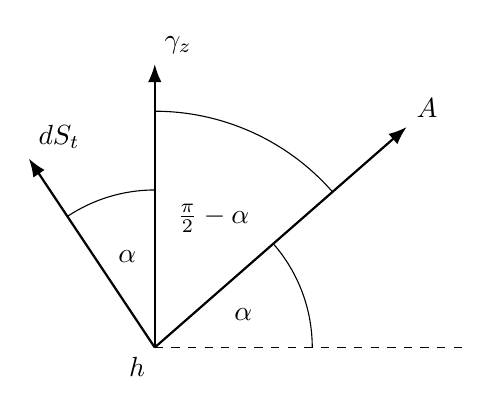
\begin{tikzpicture}[scale = 0.8]
\coordinate (O) at (0,0);
\node[anchor = north east ] at (O){$h$};
\coordinate (ds) at (-2,3);
\draw[-Latex,thick] (O)--(ds);
\node[anchor = south west ] at (ds){$dS_t$};
\coordinate (A) at (4,3.5) {};
\draw[-Latex,thick] (O)--(A);
\node[anchor = south west ] at (A){$A$};
\coordinate (gamma) at (0,4.5) {};
\draw[-Latex,thick] (O)--(gamma);
\node[anchor = south west ] at (gamma){$\gamma_z$};
 \draw pic[draw,,angle radius=3cm,"$\frac{\pi}{2}-\alpha$"] {angle=A--O--gamma};
  \draw pic[draw,,angle radius=2cm,"$\alpha$"] {angle=gamma--O--ds};
  \coordinate (P) at (5,0);
  \draw[dashed] (O)--(P);
  \draw pic[draw,,angle radius=2cm,"$\alpha$"] {angle=P--O--A};
\end{tikzpicture}
}
    \quad
\caption{Pressure on a trirectangular tetrahedron}
\label{fig:fig_p199}
\end{figure}
To see that the pressure is independent of the direction of the surface element on which we measure it, let's consider a trirectangular tetrahedron $OABC$ as  depicted in figure $6.2(a)$. Let's define $P_x,P_y,P_z, P_t$ the pressure measured on the $4$ surfaces with normal vectors $dS_x,dS_y,dS_z,dS_t$. Let's neglect second order terms due to acceleration and external forces. For the forces along axis $z$ (the same reasoning is valid for the two others) we will have $P_zdS_z= P_tdS_t\gamma_z$ where $\gamma_z$ is the cosine of the angle formed by  normal on $dS_t$ and the z-axis.\\
Let's investigate the relationship between $dS_t$ and $dS_x,dS_y,dS_z$.\\
 Be $hA$ the line element lying in the plane $ABC$ (see figure $6.2(b)$) and $hO$ the line element lying in the plane $OBC$. As the area of a triangle $=\half\times base \times perpendicular \ height$ we get $dS_z = \half |hO||BC|$. But $|hO|= |hA|\cos\alpha$  (see figure $6.2(c)$) and so $dS_z = \half |BC||hA|\cos\alpha = dS_t\gamma_z$
 and get 
\begin{align*}
&P_zdS_z= P_tdS_t\gamma_z\\ 
\Rightarrow \spatie & P_z dS_t\gamma_z= P_tdS_t\gamma_z\\ 
\Rightarrow \spatie & P_z = P_t
\end{align*}

 $$\blacklozenge$$
\newpage


\section{p201 - Exercise}
\begin{tcolorbox}
Write down the contravariant form of $\mathbf{6.147}$
$$\mathbf{6.147} \spatie \partial_t v_r + v_s v_{r|s} = X_r - \rho^{-1} p_{,r}$$
\end{tcolorbox}
\begin{align}
\mathbf{6.147} \spatie \partial_t v_r + v_s v_{r|s} &= X_r - \rho^{-1} p_{,r}\\
\times a^{mr}\spatie \partial_t a^{mr} v_r + v_s a^{mr}v_{r|s} &= a^{mr}X_r - \rho^{-1} a^{mr}p_{,r}
\end{align}
By $\mathbf{2.527}$ page 53 we  have $a^{rs}_{|t}=0$ and thus 
\begin{align}
v^{m}_{\ |s}= \left(a^{mr}v_{r}\right)_{|s} &= \left(a^{mr}\right)_{|n}v_{r}+a^{mr}v_{r|s}= a^{mr}v_{r|s} \\
(2) \Rightarrow \spatie \partial_t  v^m + v_s v^{m}_{\ \ |s} &= X^m - \rho^{-1} a^{mr}p_{,r}\\
 \Rightarrow \spatie \partial_t  v^m + v_s v^{m}_{\ \ |s} &= X^m - \rho^{-1} p^{'}_{,r}
\end{align}
Note that $p_{,r}$ in $(1)$ and $(5)$ are not the same vector function as $p_{,r}$ can be written as $\overline{\nabla}p$ which is coordinate system  dependent.
 $$\blacklozenge$$
\newpage

\section{p202 - Exercise}
\begin{tcolorbox}
Verify by means of  $\mathbf{3.204}$ that $\mathbf{6.157}$ and $\mathbf{6.156}$  are the same equation.
\end{tcolorbox}
\begin{align*}
\left\{\begin{array}{lll}
\mathbf{3.204}&\spatie&\Gamma^{n}_{rn} = \half\partial_r\log a = \partial_r\log \sqrt{a}\\
\mathbf{6.157}&\spatie&\left(\sqrt{a}a^{mn}\phi_{,m}\right)_{,n}=0\\
\mathbf{6.156}&\spatie&a^{mn}\phi_{|mn}=0
\end{array}\right.
\end{align*}
Considering also
\begin{align}
\left\{\begin{array}{l}
a^{mn}_{|k}=0\\
T^m_{|n}= \partial_n T_m+\Gamma^{m}_{kn}T_k
\end{array}\right.
\end{align}
So $\mathbf{6.156}$ can written as
\begin{align*}
& a^{mn}\phi_{|mn}=0\\
\Leftrightarrow\spatie & \left(a^{mn}\phi_{|m}\right)_{|n}=0\\
T^n = a^{mn}\phi_{|m}\spatie\Rightarrow\spatie &\partial_n T^n+\Gamma^{n}_{kn}T^k=0\\
\Rightarrow\spatie &\partial_n \left(a^{mn}\phi_{|m}\right)+\Gamma^{n}_{kn}a^{pk}\phi_{|p}=0\\
\Leftrightarrow\spatie &\partial_n \left(a^{mn}\right) \phi_{,m}+a^{mn}\phi_{,mn}+\Gamma^{n}_{kn}a^{pk}\phi_{,p}=0\\
\text{(1)}\quad \Rightarrow\spatie &\partial_n \left(a^{mn}\right) \phi_{,m}+a^{mn}\phi_{,mn}+\partial_k\log \sqrt{a}a^{pk}\phi_{,p}=0\\
\Leftrightarrow\spatie &\left(a^{mn}_{,n}\right) \phi_{,m}+a^{mn}\phi_{,mn}+\frac{1}{\sqrt{a}}\left(\sqrt{a}a^{pk}\right)_{,k}\phi_{,p}=0\\
\Leftrightarrow\spatie &\sqrt{a} \phi_{,m}\left(a^{mn}\right)_{,n}+\sqrt{a}a^{mn}\phi_{,mn}+a^{mn}\phi_{,m}\left(\sqrt{a}\right)_{,n}=0\\
\Leftrightarrow\spatie &\left(\sqrt{a}a^{mn}\phi_{,m}\right)_{,n}=0
\end{align*}
 $$\blacklozenge$$
\newpage


\section{p205 - Exercise}
\begin{tcolorbox}
Show that a small strain is a rigid body displacement if, and only if, $e_{rs}=0$. In the case of finite strain, deduce form $\mathbf{6.206}$ the conditions which must be satisfied by the partial derivatives of the displacement in order that it may b a rigid body displacement.
\end{tcolorbox}
\textbf{Suppose we deal with  a rigid body.} Then the position of two particles of the rigid body are given by

\begin{align*}
\left\{\begin{array}{l}
p_r=z_r+u_r(z)\\
p^{'}_r=z^{'}_r+u_r(z^{'})\\
\end{array}\right.
\end{align*}
and
\begin{align*}
\left\{\begin{array}{l}
L_0= z_r-z^{'}_r \\
L_1 = z^{'}_r+u_r(z^{'})-z_r-u_r(z)  
\end{array}\right.
\end{align*}
A rigid body means $L_1=L_0$, giving $u_r(z^{'})=u_r(z^{})$ i.e $u_r(z^{})$ is a constant and thus $u_{r,s}(z^{})=0$.\\
As $e_{rs}=\half\left(u_{r,s}(z^{})+u_{s,r}(z^{})\right)$ we get $e_{rs}=0$\\\\
\textbf{Suppose now that $e_{rs}=0$}\\
We have $e= e_{rs}\lambda_r\lambda_s = 0$ and $e= u_{r,s}(z^{})\lambda_r\lambda_s $. As the $\lambda_r$ are arbitrary, in the sense that we are free to choose whatever curve to approach the initial point, we conclude that $u_{r,s}(z^{})=0$ . So $u_{r}(z^{})$ is a constant, meaning that the mutual distance between two arbitrary points, do not change. The body is a rigid body.
 $$\lozenge$$
 For a finite strain we have $\mathbf{6.206}$:
 \begin{align*}
 \lim \frac{L_1^2-L_0^2}{L_0^2}=2 u_{r,s}(z^{})\lambda_r\lambda_s + u_{m,r}(z^{})u_{m,s}(z^{})\lambda_r\lambda_s
 \end{align*}
 This limit is $0$ and so we get as condition
  \begin{align*}
 \left(2 u_{r,s}(z^{}) + u_{m,r}(z^{})u_{m,s}(z^{})\right)\lambda_r\lambda_s=0
 \end{align*}
 As the $\lambda_r$ are arbitrary, in the sense that we are free to choose whatever curve to approach the initial point, we conclude that $2 u_{r,s}(z^{}) + u_{m,r}(z^{})u_{m,s}(z^{})$ must be zero.
 $$2 u_{r,s}(z^{}) + u_{m,r}(z^{})u_{m,s}(z^{})=0$$
 $$\blacklozenge$$
\newpage

\section{p207 - Clarification}
\begin{tcolorbox}
Then, clearly, since the the volume of the tetrahedron is less than $a^3$,\\\\
$\mathbf{6.217}\spatie \displaystyle \lim_{a \to 0} \frac{1}{a^2} \dv{M_r}{t}=0,\quad \displaystyle \lim_{a \to 0} \frac{1}{a^2} \int X_rdV=0$
$$\vdots$$
But  $\displaystyle \lim_{a \to 0} \frac{S}{a^2}$ is not zero,...
\end{tcolorbox}
First, note that the volume of  a trirectangular tetrahedron is $V=\frac{1}{6}abc$ with $a,b,c$ the bases of the 3 rectangular triangles (see clarification for page 199), so if $a\ge b,c$ we have  $V< a^3$.\\
There is no assurance that $\displaystyle \lim_{a \to 0} \frac{1}{a^3} \dv{M_r}{t}=0$. Indeed, consider $\mathbf{5.334}$. For a continuous medium, this equation can be written as
\begin{align*}
I_{st} &= \int_{V}\rho\epsilon_{ptq}\epsilon_{psn}z_sz_tdV
\end{align*} 
If $V$ goes to zero, the quantities under the integral can be approximated by constant values and hence, the dynamics of the tetrahedron are governed by
\begin{align*}
&\displaystyle \lim_{V \to 0}I_{st} = \rho\epsilon_{ptq}\epsilon_{psn}z_sz_t V\\
\mathbf{5.332}\text{:}\spatie &\dv{I_{st}\omega_t}{t}= M_s\\
\Rightarrow\spatie &\lim_{V \to 0} \dv{M_s}{t} = \lim_{V \to 0}V\dv{\left(\rho\epsilon_{ptq}\epsilon_{psn}z_sz_t\omega_t\right)}{t} \\
\Rightarrow\spatie &\lim_{a \to 0} \frac{1}{a^3}\dv{M_s}{t} = \lim_{a \to 0}\frac{1}{a^3}V\dv{\left(\rho\epsilon_{ptq}\epsilon_{psn}z_sz_t\omega_t\right)}{t} \\
\Rightarrow\spatie &\lim_{a \to 0} \frac{1}{a^3}\dv{M_s}{t} < \lim_{a \to 0}\frac{1}{a^3}a^3\dv{\left(\rho\epsilon_{ptq}\epsilon_{psn}z_sz_t\omega_t\right)}{t} \\
\Rightarrow\spatie &\lim_{a \to 0} \frac{1}{a^3}\dv{M_s}{t} < \lim_{a \to 0}\dv{\left(\rho\epsilon_{ptq}\epsilon_{psn}z_sz_t\omega_t\right)}{t}
\end{align*}
but there is no reason to admit that $\displaystyle \lim_{V \to 0}\dv{\left(\rho\epsilon_{ptq}\epsilon_{psn}z_sz_t\omega_t\right)}{t}=0$. \\
On the other hand, replacing $a_3$ with $a^2$ in $(5)$ gives 
\begin{align*}
&\lim_{a \to 0} \frac{1}{a^2}\dv{M_s}{t} = \lim_{a \to 0}\frac{1}{a^2}V\dv{\left(\rho\epsilon_{ptq}\epsilon_{psn}z_sz_t\omega_t\right)}{t} \\
\Rightarrow\spatie &\lim_{a \to 0} \frac{1}{a^2}\dv{M_s}{t} < \lim_{a \to 0}\frac{1}{a^2}a^3\dv{\left(\rho\epsilon_{ptq}\epsilon_{psn}z_sz_t\omega_t\right)}{t} \\
\Rightarrow\spatie &\lim_{a \to 0} \frac{1}{a^2}\dv{M_s}{t} < \lim_{a \to 0}a\dv{\left(\rho\epsilon_{ptq}\epsilon_{psn}z_sz_t\omega_t\right)}{t}\\
\Rightarrow\spatie &\lim_{a \to 0} \frac{1}{a^2}\dv{M_s}{t} =0
\end{align*}
For $ \displaystyle \lim_{a \to 0} \frac{1}{a^2} \int X_rdV=0$ the reasoning is even simpler as for a volume going to zero , we can consider $X_r$ as constant and thus 
\begin{align*}
 \displaystyle \lim_{a \to 0} \frac{1}{a^2} \int X_rdV=\displaystyle \lim_{a \to 0} \frac{1}{a^2}  X_r \int dV < \displaystyle \lim_{a \to 0} \frac{1}{a^2}  X_r a^3 = 0
\end{align*}
$$\lozenge$$
\textbf{But  $\displaystyle \lim_{a \to 0} \frac{S}{a^2}$ is not zero,...}\\\\
Be $S_t$ the area of the ``sloped'' triangle in the tetrahedron. Then, the total area of the tetrahedron is:
\begin{align*}
&S= \half\left(ab + bc + ac \right) + S_t\\
&S_t > \half ab\text{,   }S_t > \half bc\text{,   }S_t > \half ac\\
\Rightarrow \spatie & S>  \half\left(ab + bc + ac \right) + \half ab
\end{align*}
\begin{align}
\Rightarrow \spatie & \frac{S}{a^2}>  \half\left( \frac{bc}{a^2} + \frac{c}{a} \right) + b
\end{align}
If we shrink the tetrahedron uniformly and put $a=\epsilon a_0, b=\epsilon b_0, c=\epsilon c_0$ then $(1)$ can be written as 
\begin{align*}
\lim_{\epsilon \to 0}\frac{S}{a^2}>   \half\left( \frac{b_0c_0}{a_0^2} + \frac{c_0}{a_0} \right) + b_0\lim_{\epsilon \to 0}\epsilon 
\end{align*}
which is indeed not zero.
 $$\blacklozenge$$
\newpage

\section{p208 - Exercise}
\begin{tcolorbox}
Show that the stress across a plane $z_1 = \text{const.}$ has the components $E_{11}, \ E_{21}, \ E_{31}$. What are the components across planes $z_2 = \text{const.}$ and $z_3 = \text{const.}$?
\end{tcolorbox}
\begin{align*}
\mathbf{6.223} \spatie T_r = E_{rs}n_s
\end{align*}
So for the the stress across a plane $z_1 = \text{const.}$, we have $n_1=1, \ n_2=0, \ n_3 = 0$ and so 
\begin{align*}
T_r\left(z_1 = \text{const.}\right) = \left(\begin{matrix}E_{11}\\E_{21}\\E_{31}\end{matrix}\right)
\end{align*}
For the the stress across a plane $z_2 = \text{const.}$, we have $n_1=0, \ n_2=1, \ n_3 = 0$ and for the the stress across a plane $z_3 = \text{const.}$, we have $n_1=0, \ n_2=0, \ n_3 = 1$ and so
\begin{align*}
&T_r\left(z_2 = \text{const.}\right) = \left(\begin{matrix}E_{12}\\E_{22}\\E_{32}\end{matrix}\right)\\
&T_r\left(z_3 = \text{const.}\right) = \left(\begin{matrix}E_{13}\\E_{23}\\E_{33}\end{matrix}\right)\
\end{align*}
 $$\blacklozenge$$
\newpage

\section{p210 - Exercise}
\begin{tcolorbox}
Show that the if $\mathbf{6.233}$ is solved for strain, so as to read
$$\mathbf{6.237} \spatie e_{rs}= C_{rsmn}E_{mn}$$
then the symmetry conditions $\mathbf{6.234}, \  \mathbf{6.235}, \text{ and } \mathbf{6.236} $ imply similar conditions on $C_{rsmn}$. (The tensor $C_{rsmn}$ is he second elasticity tensor).
\end{tcolorbox}
\textbf{a) $C_{rsnm}= C_{rsmn}$ and $C_{srmn}= C_{rsmn}$\\}
This is a direct consequence of the symmetries $E_{nm}= E_{mn}$ and $e_{nm}= e_{mn}$. \\E.g.:
\begin{align*}
&e_{nm}= e_{mn}\\
\Leftrightarrow\spatie &C_{nmrs}E_{rs}=C_{mnrs}E_{rs}\\
\Rightarrow\spatie &C_{nmrs}=C_{mnrs}
\end{align*}\\
\textbf{b) $C_{rsnm}= C_{mnrs}$ \\}
We simplify the notation by using 'compactified' indices (e.g.):
$$e_{a}= C_{ab}E_{b} \quad \Leftrightarrow \quad e_{rs}= C_{rsmn}E_{mn}$$
Let's form the invariant $E_ae_a$, then :
\begin{align}
E_ae_a &=  c_{au}e_{u}C_{av}E_{v}\\
&=  c_{ua}e_{a}C_{uv}E_{v}\quad\text{(renaming dummy indices)}\\
&=  C_{uv}E_u E_{v}\\
&=  C_{vu}E_u E_{v}\quad\text{(renaming dummy indices)}
\end{align}
From $(3)$ and $(4)$ we can conclude 
$$C_{vu}=C_{uv}$$
 $$\blacklozenge$$
\newpage

\section{p212 - Exercise}
\begin{tcolorbox}
Deduce from  $\mathbf{6.250}$ that if an isotropic elastic body is in equilibrium under no body forces, then the expansion $\theta$ is an harmonic function $\left(\mathbf{\Delta}\theta = 0\right)$
\end{tcolorbox}
$$\mathbf{6.250}: \spatie \rho f_r= \rho X_r+\left(\lambda+ \mu\right)\theta_{,r}+\mu\mathbf{\Delta}u_r$$
In equilibrium under no body forces means $f_r=0$ and $X_r=0$. So,
\begin{align*}
&\left(\lambda+ \mu\right)\theta_{,r}+\mu\mathbf{\Delta}u_r=0\\
\partial_r \quad \Rightarrow \spatie &\left( \lambda+ \mu \right)\underbrace{\theta_{,rr}}_{= \mathbf{\Delta}\theta} +\mu\underbrace{\left(\mathbf{\Delta}u_r \right)_{,r}}_{=\mathbf{\Delta}u_{r,r}} =0\\
u_{r,r}=\theta\quad\Rightarrow\spatie &\left( \lambda+ \mu \right)\mathbf{\Delta}\theta +\mu\mathbf{\Delta}\theta =0\\
\Rightarrow\spatie & \mathbf{\Delta}\theta =0
\end{align*}
 $$\blacklozenge$$
\newpage

\section{p213 - Exercise}
\begin{tcolorbox}
Express the equations of motion   $\mathbf{6.250}$ in curvilinear coordinates.
\end{tcolorbox}
$$\mathbf{6.250}: \spatie \rho f_r= \rho X_r+\left(\lambda+ \mu\right)\theta_{,r}+\mu\mathbf{\Delta}u_r$$
We start from $\mathbf{6.252}: \spatie \rho f^r= \rho X^r+E^{rs}_{\ \ |s}$
\begin{align*}
& \rho f^r= \rho X^r+E^{rs}_{\ \ |s}\\
\mathbf{6.245}\text{:}\quad\Rightarrow\spatie & E^{rs} = \lambda \delta_{rs} \theta + 2 \mu e^{rs}\\
\Rightarrow\spatie & \rho f^r= \rho X^r+\lambda \delta_{rs} \theta _{ |s} + 2 \mu e^{rs}_{\ \ |s}\\
\Leftrightarrow\spatie & \rho f^r= \rho X^r+\lambda  \theta _{,r} + 2 \mu e^{rs}_{\ \ |s}
\end{align*}
\begin{align}
\mathbf{6.245}\text{: }\spatie \spatie & e^{rs} = \half\left(u^r_{\ |s}+u^s_{\ |r}\right)\\
\Rightarrow\spatie & \rho f^r= \rho X^r+\lambda  \theta _{,r} + 2 \mu \half\left(u^r_{\ |ss}+u^s_{\ |rs}\right)
\end{align}
\begin{align*}
\mathbf{6.246}\text{: }\spatie \spatie &\theta = e^{nn} = \half\left(u^n_{\ |n}+u^n_{\ |n}\right) = u^n_{\ |n}\\
\text{(2)}\Rightarrow\spatie & \rho f^r= \rho X^r+\lambda  \theta _{,r} + \mu \left(u^r_{\ |ss}+\theta_{\ |r}\right)\\
\Rightarrow\spatie & \rho f^r= \rho X^r+\left(\lambda +\mu\right) \theta _{,r} + \mu u^r_{\ |ss}
\end{align*}
So, $$f^r= \rho X^r+\left(\lambda +\mu\right) \theta _{,r} + \mu \mathbf {\Delta}u^r$$
where we define the Laplacian differential operator as $$\mathbf{\Delta}\left({\cdot}\right) \overset{\underset{\mathrm{def}}{}}{=} \left({\cdot}\right)_{|nn}$$
 $$\blacklozenge$$
\newpage

\section{p215 - Exercise}
\begin{tcolorbox}
Verify that $E_r=z_r, \ H_r=0$ satisfy the wave equation but not Maxwell's equations
\end{tcolorbox}
$$\mathbf{6.306}: \spatie \ \frac{1}{c^2}\frac{\partial^2E_r}{\partial t^2} -E_{r,mn} = 0$$
$$\mathbf{6.307}: \spatie \ \frac{1}{c^2}\frac{\partial^2H_r}{\partial t^2} -H_{r,mn} = 0$$
Obviously, $\mathbf{6.307}$ is trivial as $H_r=0$ is a constant $=0$, and so are the derivatives.\\
For $\mathbf{6.306}$, $ \frac{\partial^2E_r}{\partial t^2}= 0$ as $E_r$ is no function of time.\\
So, the defined field satisfy the wave equation.\\
\begin{align*}
\left\{ \begin{array}{ll}
\mathbf{6.301}: &\frac{1}{c}\frac{\partial E_r}{\partial t} = \epsilon_{rmn}H_{n,m}, \quad  \frac{1}{c}\frac{\partial H_r}{\partial t}= -\epsilon_{rmn}E_{n,m}\\
\mathbf{6.302}: & E_{n,n}=0, \spatie \quad H_{n,n}=0
\end{array}\right.
\end{align*}
The first equation of $\mathbf{6.302}$ is not satisfied as $E_{n,n}= N$ with $N$ the space dimension.
 $$\blacklozenge$$
\newpage

\section{p220 - Exercise}
\begin{tcolorbox}
Prove a similar statement for the electric and magnetic vectors of the complementary electromagnetic field.
\end{tcolorbox}
If we take the complex conjugate of $\mathbf{6.324}$ and subtract, we obtain after multiplying by $i$:
\begin{align*}
E^{**}_r = -\epsilon_{rmn}H^{**}_nV_{,m}, \quad H^{**}_r = \epsilon_{rmn}E^{**}_nV_{,m}, 
\end{align*} 

Hence, the vectors $V_{,r}, E^{**}_r$ and $ H^{**}_r$ form a right-handed orthogonal triad, and we obtain the relation
\begin{align*}
E^{**}_rE^{**}_r=H^{**}_nH^{**}_n
\end{align*}
 $$\blacklozenge$$
\newpage

\section{p221 - Clarification}
\begin{tcolorbox}
Some thoughts about polarization
\end{tcolorbox}


\begin{figure}[H]%
    \centering
    \subfloat[]{\begin{tikzpicture}[x=(15:0.5), y=(90:0.6), z=(-20:2.2)]
  \newcommand*\lateraleye{%
       \scalebox{0.25}{
    \tikzset{every picture/.style={line width=0.75pt}} 
    \begin{tikzpicture}[x=0.75pt,y=0.75pt,yscale=-1,xscale=1]
    \draw  [line width=1.5]  (300,100.33) .. controls (326,122) and (352,135) .. (378,139.33) .. controls (352,143.67) and (326,156.67) .. (300,178.33) ;
    \draw  [fill={rgb, 255:red, 0; green, 0; blue, 0 }  ,fill opacity=1 ] (308.94,116.33) .. controls (313.87,116.33) and (317.86,125.51) .. (317.85,136.83) .. controls (317.84,148.15) and (313.84,157.33) .. (308.91,157.33) .. controls (303.99,157.32) and (300,148.14) .. (300.01,136.82) .. controls (300.02,125.5) and (304.02,116.32) .. (308.94,116.33) -- cycle ;
    \draw  [draw opacity=0][line width=1.5]  (314.84,166.6) .. controls (311.87,164.64) and (309.14,162.18) .. (306.76,159.24) .. controls (295.12,144.82) and (296.6,124.33) .. (310.07,113.45) .. controls (311.48,112.32) and (312.96,111.33) .. (314.5,110.49) -- (331.14,139.55) -- cycle ; \draw  [line width=1.5]  (314.84,166.6) .. controls (311.87,164.64) and (309.14,162.18) .. (306.76,159.24) .. controls (295.12,144.82) and (296.6,124.33) .. (310.07,113.45) .. controls (311.48,112.32) and (312.96,111.33) .. (314.5,110.49) ;
    \draw  [fill={rgb, 255:red, 255; green, 255; blue, 255 }  ,fill opacity=1 ] (304.43,124.2) .. controls (306.09,124.25) and (307.32,128.01) .. (307.18,132.6) .. controls (307.05,137.19) and (305.59,140.88) .. (303.93,140.83) .. controls (302.27,140.78) and (301.03,137.02) .. (301.17,132.43) .. controls (301.31,127.83) and (302.76,124.15) .. (304.43,124.2) -- cycle ;
    \end{tikzpicture}
    }\,}
  \def\A{1.4}
  \def\L{3.0}
  \def\M{7.5}
  \def\nwave{4}
  \def\k{(360*\nwave/\M)} % 2pi*n / L = 360*n / L
  \def\nvec{40} % vectors per wavelength
  % SECTION 1
 
   \draw[thick,-Latex] (0,0,0) -- (0,0,1.2*\M);
  \draw[thick] (0,0,0) -- (0,0,0.4*\L);
  \draw[thick] (0,0,0.4*\L) -- (0,0,\L);
  \draw[->] (0,0,1.*\L)++(60:1.1*\A) --++ (0,0,0.2*\L) node[right] {$\vb{v}$};
  \node[scale=0.9,yslant=tan(0)] at (-0.8*\L,-0.8*\L,0.4*\L) {P };
  \node[scale=0.9,yslant=tan(0)] at (0,0.6*\L,0.4*\L) { $E_1$};
   \node[scale=0.9,yslant=tan(0)] at (-2.0,-0.50,0.4*\L) { $E_2$};
  \node[scale=0.9,yslant=tan(-10)] at (0,0,9.5) { $ \lateraleye$};
 
  
  % SECTION 2
  %Vertical components
  \begin{scope}[shift={(0,0,0*\L/2)}]
    \draw[samples=100,smooth,variable=\z,domain=0.4*\L:1.*\M,very thick]
      plot(0,{\A*cos(\k*\z)},\z);
    \foreach \i [evaluate={\z=\i*1.*\M/\nvec; \c=int(\i!=\nvec/2);}] in {0,...,\nvec}{
      \ifnum\c=1
        \draw[very thin] (0,0,\z) --++ (90:{\A*cos(\k*\z)});
      \fi
    }
    \draw[samples=100,smooth,variable=\z,domain=0:0.4*\L,,gray!50,thin]
      plot(0,{\A*cos(\k*\z)},\z);
    \foreach \i [evaluate={\z=\i*\M/\nvec; \c=int(\i!=\nvec/2);}] in {0,...,\nvec}{
      \ifnum\c=1
        \draw[gray!30,thin] (0,0,\z) --++ (90:{\A*cos(\k*\z)});
      \fi
    }
        \foreach \i [evaluate={\z=\i*\M/\nwave/2}] in {0,...,8}{
         \draw[fill=white]  (0,0,\z) --++ (0:0) circle (1.5pt);
    }
    \foreach \i [evaluate={\p=\i*\M/\nwave/2+\M/\nwave/4}] in {0,...,7}{
         \draw[fill=gray]  (0,0,\p) --++ (0:0) circle (1.5pt);
    }
   
    %Horizontal components
  \draw[samples=100,smooth,variable=\z,domain=0.4*\L:1.*\M,,very thick]
      plot({2*\A*cos(\k*\z+90)},0,\z);
    \foreach \i [evaluate={\z=\i*1.*\M/\nvec; \c=int(\i!=\nvec/2);}] in {0,...,\nvec}{
      \ifnum\c=1
        \draw[gray!30,thin] (0,0,\z) --++ (0:{2*\A*cos(\k*\z+90)});
      \fi
    }
     \draw[samples=100,smooth,variable=\z,domain=0:0.4*\L,gray!50,thin]
      plot({2*\A*cos(\k*\z+90)},0,\z);
    \foreach \i [evaluate={\z=\i*\M/\nvec; \c=int(\i!=\nvec/2);}] in {0,...,\nvec}{
      \ifnum\c=1
        \draw[gray!30,very thin] (0,0,\z) --++ (90:{\A*cos(\k*\z+90)});
      \fi
    }
  \end{scope}
  
  \draw[thin,dashed,] (1*\L,1*\L,0.4*\L) -- (1*\L,-1*\L,0.4*\L)--  (-1*\L,-1*\L,0.4*\L)-- (-1*\L,1*\L,0.4*\L)-- cycle;
   \draw[->, thin] (0,0,0.4*\L)++(0:0) --++ (0+180:2*\A);
  \draw[->, thin] (0,0,0.4*\L)++(90:0) --++ (90+180:\A);
  \draw[->, thin,] (0,0,0.4*\L)++(90+180:0) --++ (90+0:\A);
  \draw[->,thin] (0,0,0.4*\L)++(180:0) --++ (180+180:2*\A);
  \begin{scope}[canvas is xy plane at z=0.4*\L]
    \draw[thick,dashed] {(0,0) ellipse (2*1.4 and 1.4)};
  \end{scope}
\end{tikzpicture}    }
    \quad
        \subfloat[]{
\begin{tikzpicture}[x={(0.8cm, 0.4cm)}, y={(0.9cm, -0.3cm)}, z={(0cm,1cm)}, line cap=round, line join=round]
\tikzset{>=latex}
\tikzset{axis/.style={black, very thick, ->}}
\tikzset{ef/.style={very thick, red}}
\tikzset{vec/.style={black, -{Latex[length=0.8mm]}}}
\tikzset{every text node part/.style={align=center}}

\newcommand*\lateraleye{%
       \scalebox{0.25}{
    \tikzset{every picture/.style={line width=0.75pt}} 
    \begin{tikzpicture}[x=0.75pt,y=0.75pt,yscale=-1,xscale=1]
    \draw  [line width=1.5]  (300,100.33) .. controls (326,122) and (352,135) .. (378,139.33) .. controls (352,143.67) and (326,156.67) .. (300,178.33) ;
    \draw  [fill={rgb, 255:red, 0; green, 0; blue, 0 }  ,fill opacity=1 ] (308.94,116.33) .. controls (313.87,116.33) and (317.86,125.51) .. (317.85,136.83) .. controls (317.84,148.15) and (313.84,157.33) .. (308.91,157.33) .. controls (303.99,157.32) and (300,148.14) .. (300.01,136.82) .. controls (300.02,125.5) and (304.02,116.32) .. (308.94,116.33) -- cycle ;
    \draw  [draw opacity=0][line width=1.5]  (314.84,166.6) .. controls (311.87,164.64) and (309.14,162.18) .. (306.76,159.24) .. controls (295.12,144.82) and (296.6,124.33) .. (310.07,113.45) .. controls (311.48,112.32) and (312.96,111.33) .. (314.5,110.49) -- (331.14,139.55) -- cycle ; \draw  [line width=1.5]  (314.84,166.6) .. controls (311.87,164.64) and (309.14,162.18) .. (306.76,159.24) .. controls (295.12,144.82) and (296.6,124.33) .. (310.07,113.45) .. controls (311.48,112.32) and (312.96,111.33) .. (314.5,110.49) ;
    \draw  [fill={rgb, 255:red, 255; green, 255; blue, 255 }  ,fill opacity=1 ] (304.43,124.2) .. controls (306.09,124.25) and (307.32,128.01) .. (307.18,132.6) .. controls (307.05,137.19) and (305.59,140.88) .. (303.93,140.83) .. controls (302.27,140.78) and (301.03,137.02) .. (301.17,132.43) .. controls (301.31,127.83) and (302.76,124.15) .. (304.43,124.2) -- cycle ;
    \end{tikzpicture}
    }\,}
%Styles

\tikzset{vec/.style={black, -{Latex[length=0.8mm]}}}
\tikzset{every text node part/.style={align=center}}
	\begin{scope}[canvas is yz plane at x=6]
		\draw[thick, dashed] (-1.2,-1.2) rectangle (1.52,1.2);
		\draw[very thick,  dashed] (0,0) ellipse (0.8cm and 0.6cm);
	\end{scope}
%	% Main Axes

	
	% Propagation Direction Vector
	\draw[axis] (1,0,0) -- (8.3,0,0) node[right, black] { $ $};
	\draw[axis] (1,0,2) -- (2,0,2) node[right, black] { $\vb{v}$};
	
	
	% Correction so as the Result to Seem 3d
	\draw[very thick] (1,0,0) -- (6,0,0);
	
	% Red Line
	\draw[very thick,  variable=\t, domain=1:6, samples=300] plot (\t, {0.8*sin(deg(\t*4+90))}, {0.6*cos(deg(\t*4+90))});
	
	% Vectors from Axis to Red Line
% Vectors from Axis to Red Line
	\foreach \i [evaluate={\k = \i*4; \ii = \i;}] in {1,1.10,...,6}
	{
		\draw[very thin,gray!50] (\ii,0,0) -- +(0, {0.8*sin(deg(\k+90))}, {0.6*cos(deg(\k+90))});
	}
	\begin{scope}[canvas is yz plane at x=9]
	\node[scale=0.9,xslant = tan(-30),yslant =tan(-0)] at  (0,0,6) { $ \lateraleye$};
	\end{scope};
\end{tikzpicture}}
    \quad
        \subfloat[]{\begin{tikzpicture}[x=(15:0.5), y=(90:0.6), z=(-20:2.2)]
\newcommand*\lateraleye{%
       \scalebox{0.25}{
    \tikzset{every picture/.style={line width=0.75pt}} 
    \begin{tikzpicture}[x=0.75pt,y=0.75pt,yscale=-1,xscale=1]
    \draw  [line width=1.5]  (300,100.33) .. controls (326,122) and (352,135) .. (378,139.33) .. controls (352,143.67) and (326,156.67) .. (300,178.33) ;
    \draw  [fill={rgb, 255:red, 0; green, 0; blue, 0 }  ,fill opacity=1 ] (308.94,116.33) .. controls (313.87,116.33) and (317.86,125.51) .. (317.85,136.83) .. controls (317.84,148.15) and (313.84,157.33) .. (308.91,157.33) .. controls (303.99,157.32) and (300,148.14) .. (300.01,136.82) .. controls (300.02,125.5) and (304.02,116.32) .. (308.94,116.33) -- cycle ;
    \draw  [draw opacity=0][line width=1.5]  (314.84,166.6) .. controls (311.87,164.64) and (309.14,162.18) .. (306.76,159.24) .. controls (295.12,144.82) and (296.6,124.33) .. (310.07,113.45) .. controls (311.48,112.32) and (312.96,111.33) .. (314.5,110.49) -- (331.14,139.55) -- cycle ; \draw  [line width=1.5]  (314.84,166.6) .. controls (311.87,164.64) and (309.14,162.18) .. (306.76,159.24) .. controls (295.12,144.82) and (296.6,124.33) .. (310.07,113.45) .. controls (311.48,112.32) and (312.96,111.33) .. (314.5,110.49) ;
    \draw  [fill={rgb, 255:red, 255; green, 255; blue, 255 }  ,fill opacity=1 ] (304.43,124.2) .. controls (306.09,124.25) and (307.32,128.01) .. (307.18,132.6) .. controls (307.05,137.19) and (305.59,140.88) .. (303.93,140.83) .. controls (302.27,140.78) and (301.03,137.02) .. (301.17,132.43) .. controls (301.31,127.83) and (302.76,124.15) .. (304.43,124.2) -- cycle ;
    \end{tikzpicture}
    }\,}
\tikzstyle{platecol}=[gray!20!black!20,opacity=0.8]
\tikzstyle{platetopcol}=[gray!20!black!20,opacity=0.8]
\tikzstyle{platesidEcol}=[gray!20!black!20,opacity=0.8]
\tikzstyle{mydashed}=[dash pattern=on 1.2 off 0.7,line width=0.3]
% POLARIZER
\def\W{3.5}  % width polarizer
\def\w{0.05} % width slit
\def\l{2.9}  % length slit
\def\t{0.05}
\def\N{7}    % number of slits
  \tikzset{
  plate/.pic={
    \ifnumless{45}{#1}{
      \def\topang{#1}
    }{
      \def\topang{#1+90}
    }
    \fill[platetopcol]
      (\topang:\W/2)++(\topang-90:\W/2) --++ (0,0,-\t) --++ (\topang+90:\W) --++ (0,0,\t) -- cycle;
    \fill[platesidEcol]
      (\topang+90:\W/2)++(\topang:\W/2) --++ (0,0,-\t) --++ (\topang+180:\W) --++ (0,0,\t) -- cycle;
    \fill[platecol]
      (#1:\W/2)++(#1-90:\W/2) --++ (#1-180:\W) --++ (#1+90:\W) --++ (#1:\W) -- cycle
      \foreach \i [evaluate={\x=-\W/2+\i*\W/(\N+1);}] in {1,...,\N}{
        (#1:\l/2)++(#1+90:\x+\w/2) --++ (#1-180:\l) --++ (#1-90:\w) --++ (#1:\l) -- cycle
      };
  }
}
  \def\A{1.4}
  \def\L{3.2}
  \def\M{4.5}
  \def\nwave{4}
  \def\k{(360*\nwave/\M)} % 2pi*n / L = 360*n / L
  %\def\dx{90/\k}
  \def\nvec{40} % per wavelength
  
  % SECTION 1
  \draw[thin,dashed] (1*\L,1*\L,0.4*\L) -- (1*\L,-1*\L,0.4*\L)--  (-1*\L,-1*\L,0.4*\L)-- (-1*\L,1*\L,0.4*\L)-- (1*\L,1*\L,0.4*\L);
   \draw[thick,-Latex] (0,0,0) -- (0,0,8);
  \draw[thick] (0,0,0) -- (0,0,0.4*\L);
  %\foreach \ang in {45,90,...,360}{
    %\draw[<->,very thick,Ecol] (0,0,0.4*\L)++(\ang:\A) --++ (\ang+180:2*\A);
 % }
  \draw[-Latex,very thick,] (0,0,0.4*\L)++(0:0) --++ (0+180:1.2*\A);
  \draw[-Latex,very thick,] (0,0,0.4*\L)++(90:0) --++ (90+180:2*\A);
  \draw[-Latex,very thick,] (0,0,0.4*\L)++(90+180:0) --++ (90+0:2*\A);
  \draw[-Latex,very thick,] (0,0,0.4*\L)++(180:0) --++ (180+180:1.2*\A);
  \draw[-Latex,very thick,] (0,0,0.4*\L)++(45:0) --++ (45:0.85*\A);
  \draw[-Latex,very thick,] (0,0,0.4*\L)++(45:0) --++ (45+180:0.85*\A);
   \draw[-Latex,very thick,] (0,0,0.4*\L)++(135:0) --++ (135+180:2*\A);
    \draw[-Latex,very thick,] (0,0,0.4*\L)++(135:0) --++ (135:2*\A);

  \draw[thick] (0,0,0.4*\L) -- (0,0,\L);
  \draw[-Latex,very thick,] (0,0,1.6*\L)++(60:1.1*\A) --++ (0,0,0.2*\L) node[right] {$\vb{v}$};
  \node[scale=0.9,yslant=tan(0)] at (-0.8*\L,-0.8*\L,0.4*\L) {P };
  \node[scale=0.9,yslant=tan(10)] at (0.6,-0.75*\A,0.0*\L) { $E$};
  \node[scale=0.9,yslant=tan(-10)] at (0,0,9) { $ \lateraleye$};
  
  % SECTION 2
  \begin{scope}[shift={(0,0,\L)}]
    \pic at (0,0) {plate={90}};
    \node[scale=0.9,yslant=tan(-10),right=7,below] at (-135:0.7*\W) {Q};
    \draw[thick] (0,0,0) -- (0,0,\M/2);
    \draw[Latex-Latex,very thick,] (0,0,\M/2)++(90:\A) --++ (-90:2*\A); %-\dx
    \draw[thick,samples=100,smooth,variable=\z,domain=0:\M]
      plot(0,{\A*cos(\k*\z)},\z);
    \foreach \i [evaluate={\z=\i*\M/\nvec; \c=int(\i!=\nvec/2);}] in {0,...,\nvec}{
      \ifnum\c=1
        \draw[very thin, gray!50] (0,0,\z) --++ (90:{\A*cos(\k*\z)});
      \fi
    }
    \draw[thick] (0,0,\M/2) -- (0,0,\M);
    \node[scale=0.9,yslant=tan(-10),below=-7,align=center] at (0,-1.4*\A,0.45*\M)
      {};
  \end{scope}
  
 
\end{tikzpicture}}
    \quad
\caption{Polarization of light}
\label{fig:fig_p221}
\end{figure}
In the above figures, only the electric field is represented (the magnetic field has to be imagined perpendicular to the $E_r$ vector).\\
In figure (a) we see an elliptical polarization which occurs when the EMW can be split into two perpendicular components. When $\left|\overline{E_1}\right|= \left|\overline{E_2}\right|$, one can speak about circular polarization. Figure (b) gives a view at a certain time $t$ of the result of $\overline{E_1}+\overline{E_2}$.\\
In figure (c) an observer 'sees' in the phase wave situated at $P$, an unpolarized EMV. After passing a linear polarizing material at $Q$ the observer will 'see' the EMV oscillating only in the vertical plane along $\mathbf{v}$ 
 $$\blacklozenge$$
\newpage


\section{p221 - Exercise}
\begin{tcolorbox}
What conditions must be imposed on the fixed complex vectors $E^{(0)}_r$ and $H^{(0)}_r$ in order that the wave may be plane-polarized
\end{tcolorbox}
As stated a plane-polarized wave will have  its vectors $E^{*}_r$ and $E^{**}_r$ have the same directions and moreover the $E^{*}_r$ vector maintains a fixed directions.\\
This means that $E^{*}_r$ can be written as $E^{*}_r =  \alpha\left(z,t\right) \mathcal{E}_r$ and $E^{**}_r =  \beta\left(z,t\right) \mathcal{E}_r$ with $\alpha, \ \beta$  real valued functions and $\mathcal{E}_r$ a constant. 
Note that from the definition of $E^{*}_r$ and $E^{**}_r$ we have
\begin{align}
E^{}_r &= E^{*}_r+iE^{**}_r
\end{align}
and 
\begin{align}
 \begin{array}{l}
\text{ 6.330}\\\\
\text{  6.331}\\
\end{array}
\quad &\left\{ \begin{array}{l}
\frac{\partial E^{*}_r}{\partial t} = -\frac{2\pi c}{\lambda} E^{**}_r\\\\
\frac{\partial E^{**}_r}{\partial t} = \frac{2\pi c}{\lambda}  E^{*}_r\\
\end{array}\right.\\
\Rightarrow &\left\{\begin{array}{l}
\frac{\partial \alpha}{\partial t} = -\frac{2\pi c}{\lambda} \beta\\\\
\frac{\partial \beta}{\partial t} = \frac{2\pi c}{\lambda}  \alpha\\
\end{array}\right.\\
\Rightarrow &\left\{\begin{array}{l}
\frac{\partial^2 \alpha}{\partial t^2} = -\left(\frac{2\pi c}{\lambda}\right) ^2 \alpha\\\\
\frac{\partial^2 \beta}{\partial t^2} = -\left(\frac{2\pi c}{\lambda}\right) ^2 \beta\\\\
\end{array}\right.\\
\Rightarrow &\left\{\begin{array}{l}
\alpha = A\left(z\right)\cos \frac{2\pi c}{\lambda}  t + B\left(z\right)\sin \frac{2\pi c}{\lambda}  t \\\\
\beta = C\left(z\right)\cos \frac{2\pi c}{\lambda}  t + D\left(z\right)\sin \frac{2\pi c}{\lambda}  t   
\end{array}\right.\\
\Rightarrow \quad & \frac{E^{}_r}{\mathcal{E}_r}=A\cos \frac{2\pi c}{\lambda} t + B\sin \frac{2\pi c}{\lambda} t+i\left(C\left(z\right)\cos \frac{2\pi c}{\lambda}  t + D\left(z\right)\sin \frac{2\pi c}{\lambda}  t \right)
\end{align}
With $A,B,C,C:\mathbb{R}^3\rightarrow \mathbb{R}$.\\
Let's write $E^{(0)}_r$ as $E^{(0)}_r = a+ib$ with $a, b$ real valued functions depending on the position only.
Then, $\textbf{6.308}$ can be rewritten as
\begin{align}
E^{}_r &= \left(a+ib\right)\left(\cos S+i\sin S\right)\\
&= a\cos S-b\sin S+i\left(b\cos S+a\sin S\right)
\end{align}
We have, with $S= \frac{2\pi V}{\lambda}-\frac{2\pi c}{\lambda}t$
\begin{align}
&\left\{\begin{array}{l}
\cos S= \cos \frac{2\pi V}{\lambda}\cos \frac{2\pi c}{\lambda}t+\sin \frac{2\pi V}{\lambda}\sin \frac{2\pi c}{\lambda}t\\\\
\sin S= \sin \frac{2\pi V}{\lambda}\cos \frac{2\pi c}{\lambda}t-\cos \frac{2\pi V}{\lambda}\sin\frac{2\pi c}{\lambda}t\\
\end{array}\right.\\
\text{(8)}\Rightarrow \quad E^{}_r =& \left\{\begin{array}{l}a\cos \frac{2\pi V}{\lambda}\cos \frac{2\pi c}{\lambda}t+a\sin \frac{2\pi V}{\lambda}\sin \frac{2\pi c}{\lambda}t+b\cos \frac{2\pi V}{\lambda}\sin \frac{2\pi c}{\lambda}t-b\sin \frac{2\pi V}{\lambda}\cos \frac{2\pi c}{\lambda}t\\\\
+i\left(
b\cos \frac{2\pi V}{\lambda}\cos \frac{2\pi c}{\lambda}t+b\sin \frac{2\pi V}{\lambda}\sin \frac{2\pi c}{\lambda}t - a\cos \frac{2\pi V}{\lambda}\sin \frac{2\pi c}{\lambda}t+a\sin \frac{2\pi V}{\lambda}\cos \frac{2\pi c}{\lambda}t
\right)
\end{array}\right.\\
=& \left\{\begin{array}{l}\left(a\cos \frac{2\pi V}{\lambda}-b\sin \frac{2\pi V}{\lambda}\right)\cos \frac{2\pi c}{\lambda}t+\left(a\sin \frac{2\pi V}{\lambda}+b\cos \frac{2\pi V}{\lambda}\right)\sin \frac{2\pi c}{\lambda}t\\\\
+i\left[
\left(b\cos \frac{2\pi V}{\lambda}+a\sin \frac{2\pi V}{\lambda}\right)\cos \frac{2\pi c}{\lambda}t+\left(b\sin \frac{2\pi V}{\lambda} - a\cos \frac{2\pi V}{\lambda}\right)\sin \frac{2\pi c}{\lambda}t
\right]\\\\
\end{array}\right.
\end{align}
Let's now compare equations $(6)$ and $(11)$
\begin{align}
&E^{}_r=A\mathcal{E}_r\cos \frac{2\pi c}{\lambda} t + B\mathcal{E}_r\sin \frac{2\pi c}{\lambda} t+i\left(C\mathcal{E}_r\cos \frac{2\pi c}{\lambda}  t + D\mathcal{E}_r\sin \frac{2\pi c}{\lambda}  t \right)\\
&E^{}_r=\left\{\begin{array}{l}\left(a\cos \frac{2\pi V}{\lambda}-b\sin \frac{2\pi V}{\lambda}\right)\cos \frac{2\pi c}{\lambda}t+\left(a\sin \frac{2\pi V}{\lambda}+b\cos \frac{2\pi V}{\lambda}\right)\sin \frac{2\pi c}{\lambda}t\\\\
+i\left[
\left(a\sin \frac{2\pi V}{\lambda}+b\cos \frac{2\pi V}{\lambda}\right)\cos \frac{2\pi c}{\lambda}t-\left(a\cos \frac{2\pi V}{\lambda}-b\sin \frac{2\pi V}{\lambda}\right)\sin \frac{2\pi c}{\lambda}t
\right]\\\\
\end{array}\right.
\end{align}
We see that 
\begin{align}
&A\mathcal{E}_r= a\cos \frac{2\pi V}{\lambda}-b\sin \frac{2\pi V}{\lambda}\\
&B\mathcal{E}_r= a\sin \frac{2\pi V}{\lambda}+b\cos \frac{2\pi V}{\lambda}\\
&C=B\\
&D=-A\\
\text{(14), (15)}\quad\Rightarrow \quad &\left\{\begin{array}{l}a= A\mathcal{E}_r\cos \frac{2\pi V}{\lambda}+B\mathcal{E}_r\sin \frac{2\pi V}{\lambda}\\
b= -A\mathcal{E}_r\sin \frac{2\pi V}{\lambda}+B\mathcal{E}_r\cos \frac{2\pi V}{\lambda}\\
\end{array}\right.\\
\Rightarrow \quad E^{(0)}_r&= a+ib\\
&=\mathcal{E}_r\left(A\left(z\right)+iB\left(z\right)\right)e^{-\frac{2\pi V}{\lambda}}
\end{align}
So, the direction of $E^{(0)}_r$ does not change as $\frac{E^{(0)}_r}{E^{(0)}_s} = \frac{\mathcal{E}_r}{\mathcal{E}_s}$  and the magnitude varies with the position but in such a way that the effect of $V$ is annihilated.
$$\blacklozenge$$
\newpage

\section{p223 - Clarification}
\begin{tcolorbox}
Interrelationship between the identities $\mathbf{6.337}$ to $\mathbf{6.340}$
\end{tcolorbox}
\begin{align}
\mathbf{6.337} \spatie &\frac{1}{c^2}\frac{\partial^2 \phi_r}{\partial t^2}+ \frac{1}{c} \pdv{\psi_{,r}}{t} = \phi_{r,mm}-\phi_{m,mr}\\
\mathbf{6.338} \spatie &\frac{1}{c}\frac{\partial}{\partial t} \phi_{m,m}+ \psi_{,mm}=0\\
\mathbf{6.339(a)} \spatie &\frac{1}{c^2}\frac{\partial^2 \phi_r}{\partial t^2}-  \phi_{r,mm}=0\\
\mathbf{6.339(b)} \spatie &\frac{1}{c^2}\frac{\partial^2 \psi}{\partial t^2}-  \psi_{,mm}=0\\
\mathbf{6.340} \spatie &\frac{1}{c}\frac{\partial \psi}{\partial t}+ \phi_{m,m}=0
\end{align}
then
\begin{align}
\text{(3) in (1)}\spatie & \frac{1}{c} \pdv{\psi_{,r}}{t} =-\phi_{m,mr}\\
\pdv{\text{(5)}}{z_r}\spatie &\frac{1}{c}\frac{\partial \psi_{,r}}{\partial t}+ \phi_{m,mr}=0\quad \Leftrightarrow \quad \text{(6)}
\end{align}
What about $\text{(4)}$ ?\\
\begin{align}
\text{(4) in (2)}\spatie & \frac{1}{c}\frac{\partial}{\partial t} \phi_{m,m}=-\frac{1}{c^2}\frac{\partial^2 \psi}{\partial t^2}\\
\int_{t} \text{(8)}\Rightarrow\spatie &\frac{1}{c}\frac{\partial \psi}{\partial t}+ \phi_{m,m}=C
\end{align}
In $\text{(9)}$, $C$ is a function, constant in $t$. Imposing $C=0$ gives still a valid solution and is equivalent with $\text{(5)}$.
 $$\blacklozenge$$
\newpage


\section{p223 - Clarification}
\begin{tcolorbox}
 $$\mathbf{6.342}\spatie \frac{1}{c^2}\frac{\partial^2 \Pi_r}{\partial t^2}- \Pi_{r,mm}=0$$
\end{tcolorbox}
\begin{align}
\mathbf{6.341(a)} \spatie &\mathbf{E_n= \Pi_{m,mn}-\frac{1}{c^2}\frac{\partial^2 \Pi_n}{\partial t^2}}\\
\mathbf{6.341(b)} \spatie &\mathbf{H_n= \frac{1}{c}\epsilon_{npq}\frac{\partial}{\partial t}\Pi_{q,p}}
\end{align}
We first check, under which conditions $\text{(1) and (2)}$ satisfy the Maxwell equations 
\begin{align}\left\{ \begin{array}{ll}
\text{6.301(a),(b)}&E_{m,m}=0,\spatie H_{m,m}=0\\\\
\text{6.302(a)}&\frac{1}{c}\frac{\partial E_r}{\partial t}= \epsilon_{rmn}H_{n,m}\\\\
\text{6.302(b)}&\frac{1}{c}\frac{\partial H_r}{\partial t}= -\epsilon_{rmn}E_{n,m}
\end{array}\right.
\end{align}
with the wave equations: 
\begin{align}\left\{ \begin{array}{ll}
\text{6.306}&\frac{1}{c^2}\frac{\partial^2 E_r}{\partial t^2}- E_{r,mm}=0\\\\
\text{6.307}&\frac{1}{c^2}\frac{\partial^2 H_r}{\partial t^2}- H_{r,mm}=0
\end{array}\right.
\end{align}
We have for $\mathbf{6.301(b)}$:
\begin{align}
\text{(2)}_{,n}\spatie H_{n,n} &= \frac{1}{c}\epsilon_{npq}\frac{\partial \Pi_{q,pn}}{\partial t}\\&= 0 \quad \left(  \Pi_{q,pn}=\Pi_{q,np } \text{ and }\epsilon_{npq}=-\epsilon_{pnq} \right)\end{align}
So, $\mathbf{6.301(b)}$ is satisfied.\\\\
For $\mathbf{6.302(b)}$ we have:
\begin{align}               
\text{6.302(b)}\spatie &\frac{1}{c}\frac{\partial H_r}{\partial t}= -\epsilon_{rmn}E_{n,m}\\
\text{(2)}_{,t}\quad \Rightarrow\spatie &\frac{1}{c}\epsilon_{npq}\frac{\partial^2}{\partial t^2}\Pi_{q,p}= -\epsilon_{rmn}E_{n,m}\\
\text{(1) in (8)}\quad \Rightarrow\spatie &\frac{1}{c}\epsilon_{npq}\frac{\partial^2}{\partial t^2}\Pi_{q,p}= -\underbrace{\epsilon_{rmn}\Pi_{q,qnm}}_{=0}+\epsilon_{rmn}\frac{1}{c^2}\frac{\partial^2 \Pi_{n,m}}{\partial t^2}\\
\Rightarrow\spatie &\frac{1}{c}\epsilon_{npq}\frac{\partial^2}{\partial t^2}\Pi_{q,p}= \epsilon_{rmn}\frac{1}{c^2}\frac{\partial^2 \Pi_{n,m}}{\partial t^2}
\end{align}
So, $\mathbf{6.302(b)}$ is satisfied.\\\\
We still have to prove that the expression $\text{(1) and (2)}$ are consistent with $\text{6.301(a)}$ and $\text{6.302(a)}$\\\\
also for $\mathbf{6.301(a)}$:
\begin{align}
\text{(1)}_{,n}\spatie E_{n,n} &= \Pi_{m,mnn}-\frac{1}{c^2}\frac{\partial^2 \Pi_{n,n}}{\partial t^2}
\end{align}
and for $\mathbf{6.302(a)}$:
\begin{align}
\text{6.302(a)}\spatie \frac{1}{c}\frac{\partial E_r}{\partial t}&= \epsilon_{rmn}H_{n,m}\\
\text{(2)}\quad \Rightarrow\spatie&= \epsilon_{rmn}\frac{1}{c}\epsilon_{npq}\frac{\partial}{\partial t}\Pi_{q,pm}\\
\Rightarrow\spatie \frac{\partial E_r}{\partial t}&= \epsilon_{rmn}\epsilon_{npq}\frac{\partial}{\partial t}\Pi_{q,pm}\\
&= \left(\delta_{rp}\delta_{mq}-\delta_{rq}\delta_{mp}\right)\frac{\partial}{\partial t}\Pi_{q,pm}\\
&= \partial_t\Pi_{m,rm}-\partial_t\Pi_{r,mm}
\end{align}
Let's impose the condition on $\Pi_n$:
\begin{align}
\mathbf{6.342} \spatie &\mathbf{\Pi_{r,mm}=\frac{1}{c^2}\frac{\partial^2 \Pi_r}{\partial t^2}}
\end{align}
From $(1)$ we have
\begin{align}
\frac{1}{c^2}\frac{\partial^2 \Pi_r}{\partial t^2}&=\Pi_{m,mr}-E_r\\
\text{(17) becomes}\spatie  \Pi_{r,mm}&=\Pi_{m,mr}-E_r\\
\Rightarrow\spatie E_r &= \Pi_{m,mr}-\Pi_{r,mm}\\
\Rightarrow\spatie \partial_tE_r &=\partial_t\Pi_{m,mr}- \partial_t\Pi_{r,mm}
\end{align}
Which is consistent with $\mathbf{6.302(a)}$ following $\text{(16)}$.\\\\

For $\mathbf{6.301(a)}$ we have
\begin{align}
\text{(16)}_{,n}\quad\Rightarrow\spatie \frac{1}{c^2}\frac{\partial^2 \Pi_{n,n}}{\partial t^2}&=\Pi_{n,mmn}\\
\text{(11)}\quad\Rightarrow\spatie E_{n,n} &= \Pi_{m,mnn}-\Pi_{n,mmn}\\
&=0
\end{align}
Which is consistent with $\mathbf{6.301(a)}$\\\\

 $$\blacklozenge$$
\newpage



\section{p226 - Clarification}
\begin{tcolorbox}
 $$\mathbf{6.361}\spatie \Pi^{(0)}_r\left(z\right)= \int_{V_{\zeta}}P_r\left(\zeta\right)F\left(z, \zeta\right)dV_{\zeta}$$
\end{tcolorbox}
The reason why we can find a solution in the form $\mathbf{6.361}$ is because the condition $\mathbf{6.358}: \quad \Pi^{(0)}_{r,mm}+ k^2 \Pi^{(0)}_r = 0$ is a linear homogeneous differential equation. So any linear combination of solutions of this equation will also be a solution:\\
Be
\begin{align*}
\Pi^{(0)}_r = \overset{N}{\sum} C_n\overset{n}{\Pi}^{(0)}_r
\end{align*}
where the $\overset{n}{\Pi}^{(0)}_r$ satisfy the condition  $\overset{n}{\Pi}^{(0)}_{r,mm}+ k^2 \overset{n}{\Pi}^{(0)}_r = 0$ an are evaluated at the same point $z_r$ but at different $\zeta_n$.\\
This is the situation as illustrated in the figure $(a)$ below.
\begin{figure}[H]%
    \centering
    \subfloat[]{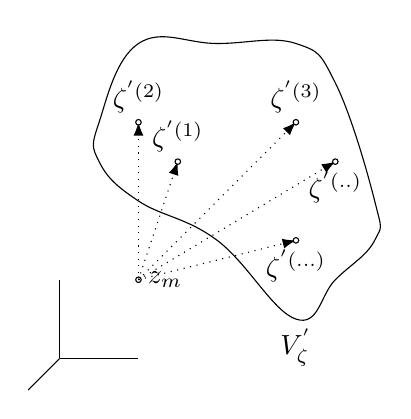
\begin{tikzpicture}
\coordinate (O) at (-0,-0);
\coordinate (X) at (-0.4-0,-0.4-0);
\coordinate (Y) at (1-0,0-0);
\coordinate (Z) at (0-0,1-0);
\draw [-](O)--(X);
\draw [-](O)--(Y);
\draw [-](O)--(Z);
\coordinate (P) at (1,1);

%First volume
\node[right] at (P) {$z_m$};
\draw  [fill= white](P)circle (1pt);
\coordinate (ksi1) at (1.5,2.5) {} {};
\coordinate (ksi2) at (1,3) {} {};
\coordinate (ksi3) at (3,3) {} {};
\coordinate (ksi4)  at (3.5,2.5) {};
\coordinate (ksi5)  at (3,1.5) {};

\node[above] at (ksi1) {$\zeta^{'(1)}$};
\node[above] at (ksi2) {$\zeta^{'(2)}$};
\node[above] at (ksi3) {$\zeta^{'(3)}$};
\node[below] at (ksi4) {$\zeta^{'(..)}$};
\node[below] at (ksi5) {$\zeta^{'(...)}$};
\draw [-Latex, dotted](P)--(ksi1);
\draw  [-Latex, dotted](P)--(ksi2);
\draw  [-Latex, dotted](P)--(ksi3);
\draw  [-Latex, dotted](P)--(ksi4);
\draw  [-Latex, dotted](P)--(ksi5);
\draw  [fill= white](ksi1)circle (1pt);
\draw  [fill= white](ksi2)circle (1pt);
\draw  [fill= white](ksi3)circle (1pt);
\draw  [fill= white](ksi4)circle (1pt);
\draw  [fill= white](ksi5)circle (1pt);
\draw  plot[smooth cycle, tension=.7] coordinates {(0.5,3) (0.5,2.5) (1,2) (2,1.5) (3,0.5) (3.5,1) (4,1.5) (4,2)  (3.5,3.5) (3,4) (2,4)   (1,4) };
\node[below] at (3,0.5){$V^{'}_{\zeta}$};

\end{tikzpicture}}
    \quad
     \subfloat[]{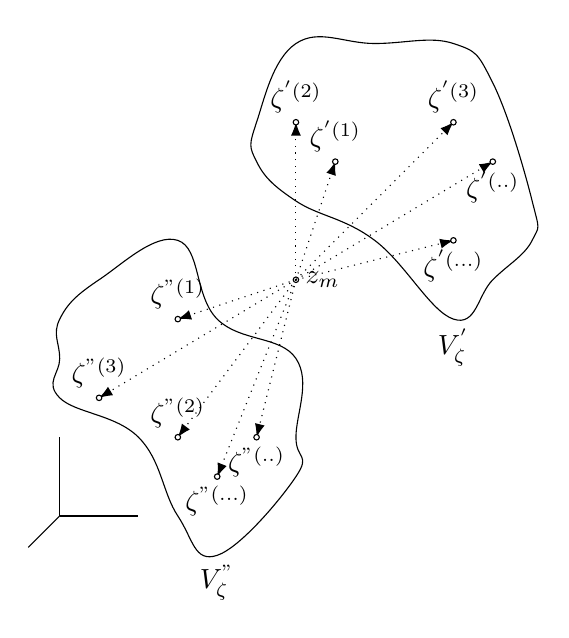
\begin{tikzpicture}
\coordinate (O) at (-2,-2);
\coordinate (X) at (-0.4-2,-0.4-2);
\coordinate (Y) at (1-2,0-2);
\coordinate (Z) at (0-2,1-2);
\draw [-](O)--(X);
\draw [-](O)--(Y);
\draw [-](O)--(Z);
\coordinate (P) at (1,1);

%First volume
\node[right] at (P) {$z_m$};
\draw  [fill= white](P)circle (1pt);
\coordinate (ksi1) at (1.5,2.5) {} {};
\coordinate (ksi2) at (1,3) {} {};
\coordinate (ksi3) at (3,3) {} {};
\coordinate (ksi4)  at (3.5,2.5) {};
\coordinate (ksi5)  at (3,1.5) {};

\node[above] at (ksi1) {$\zeta^{'(1)}$};
\node[above] at (ksi2) {$\zeta^{'(2)}$};
\node[above] at (ksi3) {$\zeta^{'(3)}$};
\node[below] at (ksi4) {$\zeta^{'(..)}$};
\node[below] at (ksi5) {$\zeta^{'(...)}$};
\draw [-Latex, dotted](P)--(ksi1);
\draw  [-Latex, dotted](P)--(ksi2);
\draw  [-Latex, dotted](P)--(ksi3);
\draw  [-Latex, dotted](P)--(ksi4);
\draw  [-Latex, dotted](P)--(ksi5);
\draw  [fill= white](ksi1)circle (1pt);
\draw  [fill= white](ksi2)circle (1pt);
\draw  [fill= white](ksi3)circle (1pt);
v\draw  [fill= white](ksi4)circle (1pt);
\draw  [fill= white](ksi5)circle (1pt);
\draw  plot[smooth cycle, tension=.7] coordinates {(0.5,3) (0.5,2.5) (1,2) (2,1.5) (3,0.5) (3.5,1) (4,1.5) (4,2)  (3.5,3.5) (3,4) (2,4)   (1,4) };
\node[below] at (3,0.5){$V^{'}_{\zeta}$};
%second volume
\coordinate (xksi1) at (-0.5,0.5) {} {} {};
\coordinate (xksi2) at (-0.5,-1) {} {} {};
\coordinate (xksi3) at (-1.5,-0.5) {} {} {};
\coordinate (xksi4) at (0.5,-1) {} {};
\coordinate (xksi5) at (0,-1.5) {} {};

\node[above] at (xksi1) {$\zeta^{{"}(1)}$};
\node[above] at (xksi2) {$\zeta^{{"}(2)}$};
\node[above] at (xksi3) {$\zeta^{{"}(3)}$};
\node[below] at (xksi4) {$\zeta^{{"}(..)}$};
\node[below] at (xksi5) {$\zeta^{{"}(...)}$};
\draw [-Latex, dotted](P)--(xksi1);
\draw  [-Latex, dotted](P)--(xksi2);
\draw  [-Latex, dotted](P)--(xksi3);
\draw  [-Latex, dotted](P)--(xksi4);
\draw  [-Latex, dotted](P)--(xksi5);
\draw  [fill= white](xksi1)circle (1pt);
\draw  [fill= white](xksi2)circle (1pt);
\draw  [fill= white](xksi3)circle (1pt);
\draw  [fill= white](xksi4)circle (1pt);
\draw  [fill= white](xksi5)circle (1pt);
\draw  plot[smooth cycle, tension=.7] coordinates {(-2,-0.5) (-1,-1)  (-0.5,-2) (0,-2.5)  (1,-1.5) (1,-1)  (1,0)  (0,0.5) (-0.5,1.5)  (-1.5,1) (-2,0.5) (-2,0) };
\node[below] at(0,-2.5){$V^{"}_{\zeta}$};
\end{tikzpicture}}
\caption{Integral form of Hertz vectors }
\label{fig:fig_p221}
\end{figure}
If we take more and more points $\zeta_r$ and take the $C_k$ as a weight  factor, then in the limit, we get $\Pi^{(0)}_r\left(z\right)= \int_{V_{\zeta}}P_r\left(\zeta\right)F\left(z, \zeta\right)dV_{\zeta}$ where $P_r\left(\zeta\right)$ is a kind of density vector field.
On page $227$, it is mentioned that the vector field $P_r\left(\zeta\right)$ does not need to be continuous. This situation is illustrated in the figure $(b)$  where $V_{\zeta} =  V^{'}_{\zeta}\oplus V^{"}_{\zeta}$
 $$\blacklozenge$$
\newpage



\section{p227 - Exercise}
\begin{tcolorbox}
Show that Maxwell's equation in the form $\mathbf{6.356}$ are satisfied by 
 $$\begin{array}{ll}& E^{(0)}_r= ik\epsilon_{rpq}\int_{V_{\zeta}}Q_q\left(\zeta\right)F_{,p}dV_{\zeta}\\
 \mathbf{6.363}&\\
 &H^{(0)}_r= \int_{V_{\zeta}}Q_m\left(\zeta\right)\left(F_{,mr}+k^2F\delta_{mr}\right) dV_{\zeta}
 \end{array}$$
 where $Q_r\left(\zeta\right)$ is an arbitrary vector field, and $F$ is as in $\mathbf{6.344}$
\end{tcolorbox}
Let's first look at this with a discrete point and define 
\begin{align}
 E^{(0)}_r&= ik\epsilon_{rpq}\Pi^{(0)}_{q,p}\\
 H^{(0)}_r&= \Pi^{(0)}_{m,mr}+k^2\Pi^{(0)}_r
\end{align}
We check whether that Maxwell's equation in the form $\mathbf{6.356}$ are satisfied:
\begin{align}
&-ikE^{(0)}_r= \epsilon_{rmn}H^{(0)}_{n,m}\\
\text{(1) and (2)}\quad\Rightarrow \spatie &-ikik\epsilon_{rpq}\Pi^{(0)}_{q,p}= \underbrace{\epsilon_{rmn}\Pi^{(0)}_{q,qmn}}_{=0}+\epsilon_{rmn}k^2\Pi^{(0)}_{n,m}\\
\Rightarrow\spatie &k^2\epsilon_{rpq}\Pi^{(0)}_{q,p}= \epsilon_{rmn}k^2\Pi^{(0)}_{n,m}
\end{align}
So the first Maxwell equation is satisfied.\\
For the second
\begin{align}
&ikH^{(0)}_r= \epsilon_{rmn}E^{(0)}_{n,m}\\
\text{(1) and (2)}\quad\Rightarrow \spatie &ik\Pi^{(0)}_{m,mr}+ik^3\Pi^{(0)}_r= \epsilon_{rmn}ik\epsilon_{npq}\Pi^{(0)}_{q,pm}\\
\Rightarrow\spatie &\Pi^{(0)}_{m,mr}+k^2\Pi^{(0)}_r= \left(\delta_{rp}\delta_{mq}-\delta_{rq}\delta_{mp}\right)\Pi^{(0)}_{q,pm}\\
\Rightarrow\spatie &\Pi^{(0)}_{m,mr}+k^2\Pi^{(0)}_r= \Pi^{(0)}_{m,mr}-\Pi^{(0)}_{r,mm}\\
\Rightarrow\spatie &\Pi^{(0)}_{r,mm}+k^2\Pi^{(0)}_r= \Pi^{(0)}_{m,mr}-\Pi^{(0)}_{m,mr}=0
\end{align}
Conclusion, $(1)$ and $(2)$ are valid expressions of a EMW provided that the condition (10) is respected.
The rest of the reasoning is identical as for  the previous form for $E^{(0)}_r$ and $H^{(0)}_r$ when we take a linear combination of $\overset{n}{\Pi}^{(0)}_r$, each satisfying (10) and taking the limit on volume $V_{\zeta}$ while expressing $\Pi^{(0)}_{r}$ as $Q_{r}\left(\zeta \right)F\left(z,\zeta\right)$.
 $$\blacklozenge$$
\newpage


\section{p228 - Exercise}
\begin{tcolorbox}
Write out Maxwell's equations in terms of a magnetic vector and a skew-symmetric electric tensor.
\end{tcolorbox}
Let's  define 
\begin{align}
 &E_{rm}= \epsilon_{rmn}E_n\\
 \Rightarrow\spatie &E_r = \half \epsilon_{rmn}E_{mn}
\end{align}
Maxwell's equation :
\begin{align}\left\{ \begin{array}{ll}
\text{6.301(a),(b)}&E_{m,m}=0,\spatie H_{m,m}=0\\\\
\text{6.302(a)}&\frac{1}{c}\frac{\partial E_r}{\partial t}= \epsilon_{rmn}H_{n,m}\\\\
\text{6.302(b)}&\frac{1}{c}\frac{\partial H_r}{\partial t}= -\epsilon_{rmn}E_{n,m}
\end{array}\right.
\end{align}\\\\
$\mathbf{6.302(a)}$:
\begin{align}
\text{6.302(a)}\times\epsilon_{rmn}\Rightarrow\spatie \frac{1}{c}\frac{\partial E_{rm}}{\partial t}&= -\epsilon_{rmn}\epsilon_{npq}H_{q,p}\\
&= \left(\delta{mp}\delta{rq}-\delta{mq}-\delta{rp}\right)H_{q,p}\\
&= H_{r,m}-H_{m,r}
\end{align}\\
So,
$$\mathbf{\frac{\partial E_{rm}}{\partial t}=H_{r,m}-H_{m,r}}$$\\
$\mathbf{6.302(b)}$:\\
\begin{align}
\text{(2) in 6.302(b)}\Rightarrow\spatie \frac{1}{c}\frac{\partial H_r}{\partial t}&= \half \epsilon_{rmn}\epsilon_{npq}E_{pq,m}\\
&= \half \left( \delta_{rp}\delta_{mq}-\delta_{rq}\delta_{pm}\right)E_{pq,m}\\
&= \half \left( E_{rm,m} -E_{mr,m}\right)\\
&= E_{rm,m} \quad\text{(}E_{rm}\text{ is skew-symmetric)}
\end{align}\\
So,
$$\mathbf{\frac{1}{c}\frac{\partial H_r}{\partial t}= E_{rm,m}}$$\\
\\\\
$\mathbf{6.301(a)}$:\\
\begin{align}
\text{(2) in 6.301(a)}\quad\Rightarrow \spatie \epsilon_{rmn}E_{mn,r}=0
\end{align}
As this equation is homogeneous, we can permute the indices in $E_{mn,r}$ and write $\epsilon_{rmn}E_{rn,m}=0$ and $\epsilon_{rmn}E_{mr,n}=0$.\\
Adding this three equation together we get 
$$\mathbf{E_{mn,r}+E_{rn,m}+E_{mr,n}=0}$$\\
\\\\
$\mathbf{6.302(b)}$:\\
As in this case, nothing changes for $H_r$ we have\\
$$\mathbf{H_{n,n}=0}$$\\
 $$\blacklozenge$$
 \newpage
 

\section{p229 - Clarification}
\begin{tcolorbox}
$$\mathbf{6.371}\spatie F_{\alpha\beta} = H_{\alpha\beta}, \ =-F_{4\alpha}=E_{\alpha}, \ F_{44}=0$$
$$\mathbf{6.374}\spatie g_{\alpha\beta} = a_{\alpha\beta}, \ g_{\alpha4}=0, \ g_{44}=-1$$
\end{tcolorbox}
For clarity this give in matrix form
\begin{align*}
\left(F_{mn}\right)=\left(\begin{matrix}
0&H_3&H_2&E_1\\
-H_3&0&H_1&E_2\\
H_2&-H_1&0&E_3\\
-E_1&-E_2&-E_3&0\\
\end{matrix}\right)
\end{align*}
\begin{align*}
\left(g_{mn}\right)=\left(\begin{matrix}
a_{11}&a_{12}&a_{13}&0\\
a_{12}&a_{22}&a_{23}&0\\
a_{13}&a_{23}&a_{33}&0\\
0&0&0&-1\\
\end{matrix}\right)
\end{align*}
 $$\blacklozenge$$
\newpage


\section{p231 - Exercise}
\begin{tcolorbox}
Show that with homogeneous coordinates $z_r$ ($z_1,z_2,z_3$ being rectangular Cartesians in space and $z_4= ict=ix^4$ ) Maxwell's equations read
$$ F_{rm,n}+F_{mn,r}+F_{nr,m}=0, \ F_{rm,m}=0$$
Write out the components of $F_{mn}$ in terms of the real electric and magnetic vectors, noting which components are real and which are imaginary.
\end{tcolorbox}
We use the same convention as in the book: Greek indices are restricted to the space manifold. Extending this manifold to a $4$ dimensional manifold, Latin suffixes will be used.
We have $\mathbf{6.369}$:
\begin{align}
\left\{\begin{array}{ll}
\text{(a)}&\frac{1}{c}\frac{\partial E_r}{\partial t}= a^{mn}H_{rm|n}\\\\
\text{(b)}&\frac{1}{c}\frac{\partial H_{rm}}{\partial t}= E_{r,m}-E_{m,r}\\\\
\text{(c)}&a^{mn}E_{n|m}=0\\\\
\text{(d)}&H_{rm,n}+H_{mn,r}+H_{nr,m}=0
\end{array}\right.
\end{align}
We rewrite (1):
\begin{align}
\left\{\begin{array}{ll}
\text{(a)}&\frac{\partial E_{\alpha}}{\partial (ict)}= -a^{\beta\gamma}H_{\alpha\beta|\gamma}\\\\
\text{(b)}&i\frac{\partial H_{\alpha\beta}}{\partial (ict)}= E_{\alpha,\beta}-E_{\beta,\alpha}\\\\
\text{(c)}&a^{\alpha\beta}E_{\beta|\alpha}=0\\\\
\text{(d)}&H_{\alpha\beta,\gamma}+H_{\beta\gamma,\alpha}+H_{\gamma\alpha,\beta}=0
\end{array}\right.
\end{align}
instead of  $\mathbf{6.371}$ let's define:
\begin{align}
&F_{\alpha\beta} =H_{\alpha\beta} , \  F_{\alpha4} =-F_{4\alpha} =-iE_{\alpha}, \ F_{44}=0\\
\Rightarrow \spatie &E_{\alpha}= iF_{\alpha4} =-iF_{4\alpha}
\end{align}

Using $(4)$, (2) becomes
\begin{align}
\left\{\begin{array}{ll}
\text{(a)}&-\frac{\partial F_{\alpha4}}{\partial (ict)}= a^{\beta\gamma}F_{\alpha\beta|\gamma}\\\\
\text{(b)}&i\frac{\partial F_{\alpha\beta}}{\partial (ict)}= iF_{\alpha4,\beta}-iF_{\beta4,\alpha}\\\\
\text{(c)}&a^{\alpha\beta}F_{\beta4,\alpha}=0\\\\
\text{(d)}&F_{\alpha\beta,\gamma}+F_{\beta\gamma,\alpha}+F_{\gamma\alpha,\beta}=0
\end{array}\right.
\end{align}
For homogeneous coordinates we have $a^{\alpha\gamma}=\delta_{\alpha\gamma}$ and $a^{\alpha4}=0$ so:
\begin{align}
\left\{\begin{array}{ll}
\text{(a)}&F_{\alpha4,4}= -F_{\alpha\beta|\beta}\\\\
\text{(b)}& F_{\alpha\beta,4}= F_{\alpha4,\beta}-F_{\beta4,\alpha}\\\\
\text{(c)}&F_{\beta4,\beta}=0\\\\
\text{(d)}&F_{\alpha\beta,\gamma}+F_{\beta\gamma,\alpha}+F_{\gamma\alpha,\beta}=0
\end{array}\right.
\end{align}

Let's look what happens when we extend the range  $\alpha,\beta,\gamma$ to $4$. First let's extend  $\gamma$ to $4$. The left part of equation (6d) can be written as 
\begin{align}
\underbrace{F_{\alpha\beta,\gamma}+F_{\beta\gamma,\alpha}+F_{\gamma\alpha,\beta}}_{=0}+ F_{\alpha\beta,4}+F_{\beta4,\alpha}+F_{4\alpha,\beta}
\end{align}
Consider 
\begin{align}
P= F_{\alpha\beta,4}+F_{\beta4,\alpha}+F_{4\alpha,\beta}
\end{align}
Let's extend $\alpha$ to $4$:
\begin{align}
P^{'}&= F_{4\beta,4}+F_{\beta4,4}+\underbrace{F_{44,\beta}}_{=0}\\
&= \underbrace{F_{4\beta,4}+F_{\beta4,4}}_{=0}\quad \text{(}F_{mn} \text{ is skew-symmetric)}
\end{align}
Extend $\beta$ to $4$:
\begin{align}
P^{"}&= F_{44,4}+F_{44,4}+F_{44,4}\\
&=0\quad \text{(}F_{mn} \text{ is skew-symmetric)}
\end{align}
This means that expression $(7)$ can be written as 
$$F_{rm,n}+F_{mn,r}+F_{nr,m}=\underbrace{F_{\alpha\beta,\gamma}+F_{\beta\gamma,\alpha}+F_{\gamma\alpha,\beta}}_{=0}+P+\underbrace{P^{'}+P^{"} }_{=0}$$
So, we only have to prove that $P= F_{\alpha\beta,4}+F_{\beta4,\alpha}+F_{4\alpha,\beta}=0$.\\
From $(6b)$ we get:
\begin{align}
P&= F_{\alpha\beta,4}+F_{\beta4,\alpha}+F_{4\alpha,\beta}\\
&= F_{\alpha4,\beta}-F_{\beta4,\alpha}+F_{\beta4,\alpha}-F_{\alpha4,\beta}\\
&=0
\end{align}
We get so by extending the indexes to $4$: ,
\begin{align}
F_{rm,n}+F_{mn,r}+F_{nr,m}=0
\end{align}
Consider now equation $(6c)$ and extend the suffixes from $3$ to $4$.\\
What is the value of the following expression?
\begin{align}
Q&=F_{4m,m}=\underbrace{F_{4\beta,\beta} }_{=0\text{ (see 6d) }}+ F_{44,4}
\end{align}
Obviously, $F_{mn}$ being skew-symmetric we have $F_{44}=0\quad\Rightarrow\quad F_{44,4}=0 \quad \Rightarrow\quad Q=0$.\\
From $\mathbf{6.378(b)}$ page 230 we know
\begin{align}
g^{\gamma\beta}F_{\alpha\gamma|\beta}=F_{\alpha\beta|\beta}=0
\end{align}
So, considering $(16)$, $(17)$ and $ (18)$ we see that the Maxwell equations reduce to 
\begin{align}\left\{\begin{array}{l}
F_{rm,n}+F_{mn,r}+F_{nr,m}=0\\
F_{rm,m}=0
\end{array}\right.
\end{align}
For the explicit expression of $F_{mn}$ we get from $(3)$ and $(4)$:
\begin{align}
F_{mn}=
\left(
\begin{matrix}
0&H_3&-H_1&-iE_1\\
-H_3&0&H_2&-iE_2\\
H_1&-H_2&0&-iE_3\\
iE_1&iE_2&iE_3&0\\
\end{matrix}
\right)
\end{align}
 $$\blacklozenge$$
\newpage



\section{p234 - Exercise 1}
\begin{tcolorbox}
For a fluid in motion referred to curvilinear coordinates, the kinetic energy of the fluid in any region $R$ is
$$T=\half\int_R\rho v_rv^rdV$$
Use the equation of motion $\mathbf{6.147}$ to show that, if we follow the particles which compose $R$, we have 
$$\dv{T}{t}= -\int_S p n_r v^rdS + \int_R \theta pdV + \int_R\rho v_rX^rdV$$
where $S$ is the bounding surface to $R$, and $n_r$ the unit vector normal to $S$ and drawn outward. Show further that if, instead of following the particles, we calculate the rate of change of $T$ for a fixed portion of space, we get the above expression with the following additional term $$ -\half\int_S\rho n_rv^rv_sv^sdS$$
\end{tcolorbox}
Let's recall that 
\begin{align}
\theta = v^r_{\ |r}\spatie  \mathbf{(6.126}\text{ page 196.)}
\end{align}
and
\begin{align}
\left\{\begin{array}{lll}
\text{(a)}&\frac{\partial v_r}{\partial t}+v^s v_{r|s} = X_r-\rho^{-1}p_{,r}&\quad \text{see (6.147)}\\\\
\text{(b)}&\frac{\partial v^r}{\partial t} + v_s v^{r}_{\ \ |s} = X^r - \rho^{-1} a^{rm}p_{,m}&\quad \text{ see exercise page 201}
\end{array}\right.
\end{align}
First let us note that, for the first part of the question, we move with the particles which means that for the considered region the mass contained in this region will remain unchanged and hence $\rho dV$ can be considered as a constant when bringing the derivation operator inside the volume integral.\\
So,
\begin{align}
T=\half\int_R\rho v_rv^rdV
\end{align}
\begin{align}
\Rightarrow\spatie\dv{T}{t} &=\half\int_R \left(\fdv{v_r}{t}v^r+\fdv{v_r}{t}v^r\right) \rho dV\\
&=\half\int_R \left[\left(\partial_t v_r+v^s v_{r|s}\right)v^r+v_r\left( \partial_t v^r + v_s v^{r}_{\ \ |s} \right)\right] \rho dV\\
&=\half\int_R \left[\left(X_r-\rho^{-1}p_{,r}\right)v^r+v_r\left(X^r - \rho^{-1} a^{rm}p_{,m}\right)\right] \rho dV\\
&=\half\int_R \left(\underbrace{X_rv^r}_{=X^rv_r}-\rho^{-1}p_{,r}v^r+X^rv_r - \rho^{-1} a^{rm}v_r p_{,m}\right) \rho dV\\
&=-\half\int_R \left(p_{,r}v^r + \underbrace{a^{rm}v_r}_{= v^m} p_{,m}\right)  dV+\int_R\rho X^rv_r dV\\
&=-\int_R p_{,r}v^r dV+\int_R \rho X^rv_r dV
\end{align}
Let's look at the expression $p_{,r}v^r$ in the first integral in (9).\\
Obviously:
\begin{align}
&\left(pv^r\right)_{,r} = p_{,r}v^r+pv^r_{,r}\\
\Rightarrow \spatie&p_{,r}v^r = \left(pv^r\right)_{,r} -pv^r_{,r}
\end{align}
Let's note also that
\begin{align}
\left(pv^r\right)_{|r} -pv^r_{\ |r} &=  \left(pv^r\right)_{,r} +\Gamma^{r}_{mr}\left(pv^m\right)-pv^r_{,r}-p\Gamma^{r}_{mr}v^m \\
&=  \left(pv^r\right)_{,r}-pv^r_{,r} \\
\text{(11) becomes}\spatie p_{,r}v^r&=\left(pv^r\right)_{|r} -pv^r_{\ |r}
\end{align}
Substituting in (9):
\begin{align}
\dv{T}{t} &=-\int_R \left(pv^r\right)_{|r} dV+\int_R pv^r_{\ |r} dV+\int_R \rho X^rv_r dV 
\end{align}
Using Green's theorem $ \int F_rn^rdS = \int F^r_{\ |r}dV$, and putting $ F^r=pv^r$:  
\begin{align}
\dv{T}{t} &=-\int_S p\underbrace{v_r n^r}_{=v^r n_r } dS+\int_R p\underbrace{v^r_{\ |r}}_{=\theta} dV+\int_R \rho X^rv_r dV 
\end{align}
giving
\begin{align}
\mathbf{\dv{T}{t} =-\int_S p v^r n_rdS+\int_R p\theta dV+\int_R \rho X^rv_r dV} 
\end{align}
$$\lozenge$$\\\\
What if we look at the rate of change of $T$ in a fixed region?\\
Then $\rho dV$ can't be considered as a constant and bringing the derivative operator under the integral will generate an additional term
\begin{align}
\half\int_R v_rv^r \fdv{\rho}{t} dV
\end{align}
As we fix the spatial coordinates, we have $\fdv{\rho}{t}= \partial_t \rho$ and by $\mathbf{6.127b}$ we have 
\begin{align}
\partial_t \rho= -\left(\rho v^r\right)_{|r}
\end{align}
So $(18)$ becomes
\begin{align}
\text{(18)}=-\half\int_R v_sv^s \left(\rho v^r\right)_{|r} dV
\end{align}
Using again Green's theorem $ \int F_rn^rdS = \int F^r_{\ |r}dV$ with   $ F^r=\rho v^r$ and nothing that $v_sv^s$ is an invariant: 
\begin{align}
\text{(18)}=-\half\int_S v_sv^s \rho v^rn_r dV
\end{align}
 $$\blacklozenge$$
\newpage



\section{p235 - Exercise 2}
\begin{tcolorbox}
Consider a fluid in which $\rho$ is a function of $p$, moving under a conservative body force. Show that if the motion is steady, but not necessarily irrotational, then the following quantity is constant along each stream line:
$$\half v_rv^r+P+U$$
(a stream line is a curve which, at each point , has the direction of the velocity vector $v^r$).
Compare and contrast this result with $\mathbf{6.154}$.
\end{tcolorbox}
What is given:

\begin{align}
\left\{\begin{array}{lll}
\text{(a)}&\partial_t v_r + v^sv_{r|s} = X_r- \rho^{-1} p_{,r}&\quad \text{see (6.147)}\\\\
\text{(b)}&P_{,r}= \rho^{-1} p_{,r}&\quad \text{ see (6.150)}\\\\
\text{(c)}&X_{r}= -U_{,r}&\quad \text{ see (6.151)}
\end{array}\right.
\end{align}
As the motion is stationary: $ \partial_t v_r =0$ and so .
\begin{align}
v^sv_{r|s} + U_{,r}+P_{,r}= 0
\end{align}

Let's consider a stream line given by the set of equations $x^r = x^r(u)$, where $u$ is a parameter. Then, by definition of a streamline, and considering a steady flow, we have $\dv{x^r}{u} = kv^r$. Considering $(2)$ we have 
\begin{align}
&v^sv_{r|s} + U_{,r}+P_{,r}= 0\\
\times \dv{x^r}{u} \spatie &v^sv_{r|s}\dv{x^r}{u} + U_{,r}\dv{x^r}{u}+P_{,r}\dv{x^r}{u}= 0\\
\spatie &v^sv_{r|s}\dv{x^r}{u} + \dv{U}{u}+\dv{P}{u}= 0
\end{align}
Let's look at the first term:
\begin{align}
v^sv_{r|s}\dv{x^r}{u}&=kv^sv_{r|s}v^r\\
&=kv^s\left(a_{rm}v^m\right)_{|s}v^r\\
&=kv^sv^m_{\  |s}a_{rm}v^r\\
&=kv^sv^m_{\ |s}v_m\\
&=kv^sv^r_{\ |s}v_r
\end{align}
So (5) can be equivalently written as $kv^sv_{r|s}v^r + \dv{U}{u}+\dv{P}{u}= 0$ and $kv^sv^r_{\  |s}v_r+ \dv{U}{u}+\dv{P}{u}= 0$.\\
 Summing these two gives
\begin{align}
&kv^s\left(v_{r|s}v^r+ v^r_{\  |s}v_r\right) + 2\dv{U}{u}+2\dv{P}{u}= 0\\
\Leftrightarrow\spatie &kv^s\left(v_{r}v^r\right)_{|s} + 2\dv{U}{u}+2\dv{P}{u}= 0\\
\Leftrightarrow\spatie &kv^s\left(v_{r}v^r\right)_{,s} + 2\dv{U}{u}+2\dv{P}{u}= 0\spatie v_{r}v^r \text{ is an invariant}\\
\Leftrightarrow\spatie &\dv{x^s}{u}\left(v_{r}v^r\right)_{,s} + 2\dv{U}{u}+2\dv{P}{u}= 0\\
\Leftrightarrow\spatie &\dv{\left(v_{r}v^r\right)}{u} + 2\dv{U}{u}+2\dv{P}{u}= 0
\end{align}
Integrating expression (15) gives 
$$\mathbf{\half v_{r}v^r + U+P= C}$$
with $C$ a constant along a streamline.
$$\lozenge$$
Compare and contrast this result with $\mathbf{6.154}$ (irrotational motion).
$$-\partial_t\phi + \half a^{mn}\phi_{,m}\phi_{,n}+P+U=F(t)$$
For a stationary motion ($\partial_t\phi=0, \ F(t)=constant$) the expression reduces to 
$$\mathbf{\half a^{mn}\phi_{,m}\phi_{,n}+P+U=C}$$
Replacing in the general expression $\half v_{r}v^r + U+P= C$, $v_{r}v^r $ by $v_r = -\phi_{,r}$ and $v^r = -a^{rm}\phi_{,m}$ gives obviously $\half a^{mn}\phi_{,m}\phi_{,n}+P+U=C$.
 $$\blacklozenge$$
\newpage



\section{p235 - Exercise 3}
\begin{tcolorbox}
For the general motion of the fluid described in Exercise 2, prove that $$\dv{}{t}\int_C v_rdx^r =0$$
where the integral is taken around any closed curve, and $\dv{}{t}$ is the co-moving time derivative.
\end{tcolorbox}

\begin{figure}[H]%
    \centering
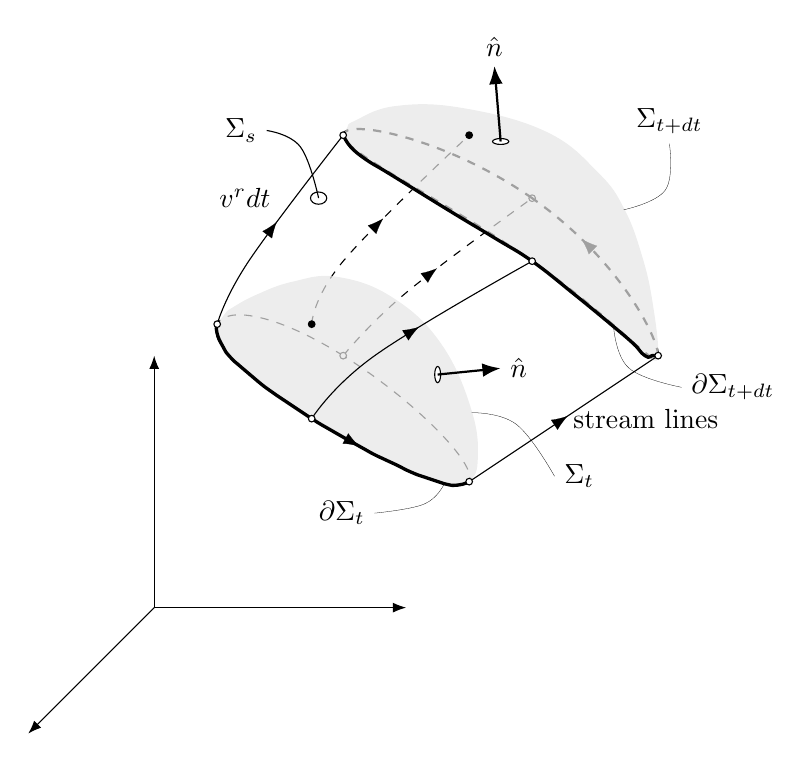
\begin{tikzpicture}[scale = 0.8]
\coordinate (O) at (-15,-5) ;
\coordinate (X) at (-17,-7) ;
\coordinate (Y) at (-11,-5) ;
\coordinate (Z) at (-15,-1) ;
\draw[-Latex] (O)--(X);
\draw [-Latex](O)--(Y);
\draw [-Latex](O)--(Z);
\coordinate (p1) at (-10,-3)  ;
\coordinate (p2) at (-12,-1)  ;
\coordinate (p3) at (-14,-0.5)  ;
\coordinate (p4) at (-12.5,-2) ;
\coordinate(pin) at (-12.5,-0.5) {};
\coordinate(pinb) at (-10,2.5) {};

\coordinate (p1b) at (-7,-1) {} {} {};
\coordinate (p2b) at (-9,1.5) {} {} {} {} {};
\coordinate (p3b) at (-12,2.5) {} {} {} {};
\coordinate (p4b) at (-9,0.5) {} {};
\draw[dashed]  [decoration={markings, mark=at position 0.52 with {\arrow[scale = 0.1]{Latex[length=20mm]}}},    postaction={decorate}]  plot[smooth, tension=.7]   coordinates {(pin) (-12,0.5) (pinb)};
\draw[dashed]     plot[smooth cycle, tension=1.] coordinates {(p1) (p2) (p3) (p4) };

\draw[dashed]  [decoration={markings, mark=at position 0.52 with {\arrow[scale = 0.1]{Latex[length=20mm]}}},    postaction={decorate}]  plot[smooth, tension=.7]   coordinates {(p2) (-11,0) (p2b)};
\draw  [fill= white](p2)circle (1.5pt);
\draw  [fill= white](p2b)circle (1.5pt);

\draw[dashed, thick,decoration={markings, mark=at position 0.92 with {\arrow[scale = 0.1]{Latex[length=20mm]}}},    postaction={decorate}]   plot[smooth cycle, tension=1] coordinates {(p1b) (p2b) (p3b) (p4b)};
\path[fill=gray!20,opacity=0.7]  plot[smooth, tension=.7] coordinates {(p3) (-14.003,-0.6401) (-13.9067,-0.8602) (-13.7967,-1.0184) (-13.6179,-1.1834) (-13.3428,-1.4172) (-13.1227,-1.5823) (-12.8682,-1.7542) (p4) (-12.1736,-2.1944) (-11.6991,-2.4626) (-11.4584,-2.5933) (-11.1764,-2.724) (-10.9082,-2.8546) (-10.6606,-2.944) (-10.3924,-3.0334) (-10.1792,-3.0541) (p1) (-9.865,-2.6831) (-9.9558,-1.8885)   (-10.4377,-0.8215) (-11.2083,-0.0814) (-12.0901,0.2502)  (-12.8008,0.1747) (-13.3825,-0.0349)   (-13.776,-0.2481) (-13.8723,-0.3306) (-13.9961,-0.4957) (-13.9961,-0.4957)};
%\draw[thin,gray,]  plot[smooth, tension=.7] coordinates { (p1) (-10.0193,-2.5059) (-10.131,-2.16) (-10.3511,-1.7828) (-10.6262,-1.3829) (-10.86,-1.039) (-11.2451,-0.6263) (-11.7128,-0.3237) (-12.1874,-0.1656) (-12.5381,-0.1037) (-12.9094,-0.0418) (-13.2396,-0.0624) (-13.556,-0.1449) (-13.776,-0.2481) (-13.8723,-0.3306) (-13.9961,-0.4957) (-13.9961,-0.4957)};
\path [fill=gray!20,opacity=0.7,line width=0pt]  plot[smooth cycle, tension=.7] coordinates {(p3b) (-11.8795,2.312) (-11.6342,2.1106) (-11.2576,1.8828) (-10.3204,1.3047) (-9.5934,0.8668) (p4b) (-8.3408,-0.0179) (-7.7014,-0.5435) (-7.3773,-0.8238) (-7.2634,-0.9551) (-7.1583,-1.0252) (p1b) (-7.0883,-0.1561) (-7.2547,0.5797) (-7.535,1.3242) (-7.9467,1.9003) (-8.7701,2.552)    (-10.1102,2.9323) (-11.1788,2.9614) (-11.8269,2.7229) (-11.9321,2.6266) (-12.0021,2.4952)};
%\draw[thin,gray,] plot[smooth , tension=.7] coordinates {(p1b) (-6.9306,-0.5172) (-7.1671,0.5952) (-7.4211,1.296) (-7.9467,1.9003) (-8.4634,2.3558) (-9.2167,2.8814) (-9.8649,3.0828) (-10.5744,3.0916) (-11.1262,2.9945) (-11.4941,2.8543) (-11.8269,2.7229) (-11.9321,2.6266) (-12.0021,2.4952)};

%\node[above] at (p1) {$p_1$};
%\node[above] at (p2) {$p_2$};
%\node[above] at (p3) {$p_3$};
%\node[above] at (p4) {$p_4$};

%\node[above] at (p1b) {$p_1$};
%\node[above] at (p2b) {$p_2$};
%\node[above] at (p3b) {$p_3$};
%\node[above] at (p4b) {$p_4$};


\coordinate (Cdt) at (-6.626,-1.5028) {} {} {} {} {};
\node[right] at (Cdt) {$\partial\Sigma_{t+dt}$};

\coordinate (C) at (-11.5,-3.5) {} {} {} {} {} {} {};
\node[left] at (C) {$\partial\Sigma_t$};
\node[right] at (-8.5,-2) {stream lines};
\node[left] at (-13,1.5) {$v^rdt$};
\coordinate (sigma_dt) at (-6.8209,2.3645) ;
\coordinate (sigma_t)  at (-8.645,-2.9141) ;
\coordinate (sigma_s)  at(-13.2133,2.5744);
\node[right] at (sigma_t) {$\Sigma_t$};
\node[above] at (sigma_dt) {$\Sigma_{t+dt}$};
\node[left] at (sigma_s) {$\Sigma_{s}$};

%\draw[dashed]    plot[smooth, tension=.7]   coordinates {(pin) (-12,0.5) (-10.8634,1.6719)};
\draw [decoration={markings, mark=at position 0.52 with {\arrow[scale = 0.1]{Latex[length=20mm]}}},    postaction={decorate}]  plot[smooth, tension=.7]   coordinates {(p3) (-13.5,0.5) (p3b)};
\draw [decoration={markings, mark=at position 0.52 with {\arrow[scale = 0.1]{Latex[length=20mm]}}},    postaction={decorate}]  plot[smooth, tension=.7]   coordinates {(p4) (-11.5,-1) (p4b)};
\draw[decoration={markings, mark=at position 0.52 with {\arrow[scale = 0.1]{Latex[length=20mm]}}},    postaction={decorate}]  plot[smooth, tension=.7]  coordinates {(p1) (-8.5,-2) (p1b)};

\draw  [fill= black](pinb)circle (1.5pt);
\draw  [fill= black](pin)circle (1.5pt);
\draw [very thick]  plot[smooth , tension=0.7] coordinates {(p3b) (-11.8795,2.312) (-11.6342,2.1106) (-11.2576,1.8828) (-10.3204,1.3047) (-9.5934,0.8668) (p4b) (-8.3408,-0.0179) (-7.7014,-0.5435) (-7.3773,-0.8238) (-7.2634,-0.9551) (-7.1583,-1.0252) (-7.1,-1)(p1b) };
\draw [very thick,decoration={markings, mark=at position 0.62 with {\arrow[scale = 0.1]{Latex[length=20mm]}}},    postaction={decorate}]   plot[smooth, tension=1.] coordinates {(p3) (-14.003,-0.6401) (-13.9067,-0.8602) (-13.7967,-1.0184) (-13.6179,-1.1834) (-13.3428,-1.4172) (-13.1227,-1.5823) (-12.8682,-1.7542) (p4) (-12.1736,-2.1944) (-11.6991,-2.4626) (-11.4584,-2.5933) (-11.1764,-2.724) (-10.9082,-2.8546) (-10.6606,-2.944) (-10.3924,-3.0334) (-10.1792,-3.0541) (p1) };



\draw  [fill= white](p1)circle (1.5pt);

\draw  [fill= white](p3)circle (1.5pt);
\draw  [fill= white](p4)circle (1.5pt);
\draw  [fill= white](p1b)circle (1.5pt);
\draw  [fill= white](p3b)circle (1.5pt);
\draw  [fill= white](p4b)circle (1.5pt);

\draw[ultra thin]  plot[smooth, tension=.7] coordinates {(-10.4045,-3.0513) (-10.7193,-3.358) (C)};
\draw[ultra thin]  plot[smooth, tension=.7] coordinates {(Cdt) (-7.4666,-1.1949) (-7.7087,-0.533)};
\draw[ultra thin]  plot[smooth, tension=.7] coordinates {(sigma_t) (-9.2503,-2.0908) (-9.9606,-1.9052)};
\draw [ultra thin] plot[smooth, tension=.7] coordinates {(sigma_dt) (-6.8854,1.6301) (-7.5473,1.3153)};

\draw  (-12.39,1.5009) node (v1) {} ellipse (0.1291 and 0.0969);

\draw  plot[smooth, tension=.7] coordinates {(sigma_s) (-12.6806,2.316) (v1)};
\coordinate (n2a) at (-9.5,2.4) {};
\coordinate (n2b) at (-9.6,3.6) {} {};
\node[above] at (n2b) {$\hat{n}$};
\draw  [fill= white](n2a)ellipse (0.1291 and 0.0469);
\draw[thick, -Latex](n2a)--(n2b);
\coordinate (n1a)  at (-10.5,-1.3) {};
\coordinate (n1b) at (-9.5,-1.2) {} {};
\node[right] at (n1b) {$\hat{n}$};
\draw  [fill= white](n1a)ellipse ( 0.0469 and 0.1291);
\draw[thick, -Latex](n1a)--(n1b);
\end{tikzpicture}
\caption{Evolution of a closed co-moving curve }
\label{fig:fig_p2235}
\end{figure}
Let's see what happens when a closed  curve moves during a time $dt$. All the particles along that curve $\partial\Sigma_t$ will move along stream lines and will form a new closed curve $\partial\Sigma_{t+dt}$. Also all particles lying on a surface $\Sigma_t$ enclosed by the closed curve will end on the surface $\Sigma_{t+dt}$.
So we can use the Kelvin-Stokes theorem and form
\begin{align}
\oint_{\partial\Sigma_{t+dt} }{v_rdx^r }-\oint_{\partial\Sigma_{t}} v_rdx^r&= \iint_{\Sigma_{t+dt}}\epsilon_{rjk}v_{k,j}n^rdS-\iint_{\Sigma_{t}}\epsilon_{rjk}v_{k,j}(n^r)dS
\end{align}

Consider now the surface formed by the envelope of the stream lines starting from the curve $\partial\Sigma_t$.

What we try to achieve is to go from a curve integral to a volume integral using first the Kelvin-Stokes theorem followed by the divergence theorem and adding a term which we have to prove it is equal to zero.\\
We write tentatively,
\begin{align}
\oint_{\partial\Sigma_{t+dt} }{v_rdx^r }-\oint_{\partial\Sigma_{t}} v_rdx^r&= \iint_{\Sigma_{t+dt}}\epsilon_{rjk}v_{k,j}n^rdS-\iint_{\Sigma_{t}}\epsilon_{rjk}v_{k,j}(-n^r)dS+\underbrace{\iint_{\Sigma_{s}}\epsilon_{rjk}v_{k,j}n^rdS}_{=0?}\\
&= \iint_{\Sigma_{t+dt}}\epsilon_{rjk}v_{k,j}n^rdS+\iint_{\Sigma_{t}}\epsilon_{rjk}v_{k,j}n^rdS+\underbrace{\iint_{\Sigma_{s}}\epsilon_{rjk}v_{k,j}n^rdS}_{=0?}\\
&= \iiint_V \epsilon_{rjk}v_{k,jr}dV\\
&=0
\end{align}
Note that in the second term of the right expression, we changed the sign of the normal vector $\hat{n}$ as we want the normal vector on the surface point outward of the considered volume.\\\\

So we have to prove that indeed,

\begin{align}\iint_{\Sigma_{s}}\epsilon_{rjk}v_{k,j}n^rdS=0\end{align}
Nothing that $n^rdS$ can be expressed as the cross product of $\overline{v}dt$ and $d\overline{l}$ (the last being the line segment along the curve $\partial_t\Sigma$), we have  
\begin{align}
n^rdS&= \epsilon_{rpq}v^pdx^qdt
\end{align}
And get
\begin{align}
\iint_{\Sigma_{s}}\epsilon_{rjk}v_{k,j}n^rdS&= \iint_{\Sigma_{s}}\epsilon_{rjk}v_{k,j}\epsilon_{rpq}v^pdx^qdt\\
&= \iint_{\Sigma_{s}}\left(\delta_{jp}\delta_{kq}-\delta_{jq}\delta_{kp}\right)v_{k,j}v^pdx^qdt\\
&= \iint_{\Sigma_{s}}\left(v_{q,p}v^pdx^q-v_{p,q}v^pdx^q\right)dt\\\left(v_pdt = dx^p\right)\quad\Rightarrow\spatie
&= \iint_{\Sigma_{s}}\left(v_{q,p}dx^pdx^q-v_{p,q}dx^pdx^q\right)\\
&=0
\end{align}
So $(5)$ is proven and get $d\oint_{\partial\Sigma_{t}} v_rdx^r=0$ during an infinitesimal time $dt$ giving 
$$\dv{}{t}\oint_{\partial\Sigma_{t}} v_rdx^r=0$$
 $$\blacklozenge$$
\newpage


\section{p235 - Exercise 4}
\begin{tcolorbox}
Curves having at each point the direction of the vorticity vector $\omega^r$ are called ``vortex lines''. Prove that $\int_{C} v_rdx^r$ has the same value for all closed curves $C$ which lie on the surface of the tube of vortex lines, and go once around the tube in the same sense. (Use Stokes' theorem; cf. 7.502.).
\end{tcolorbox}
\begin{figure}[H]%
    \centering
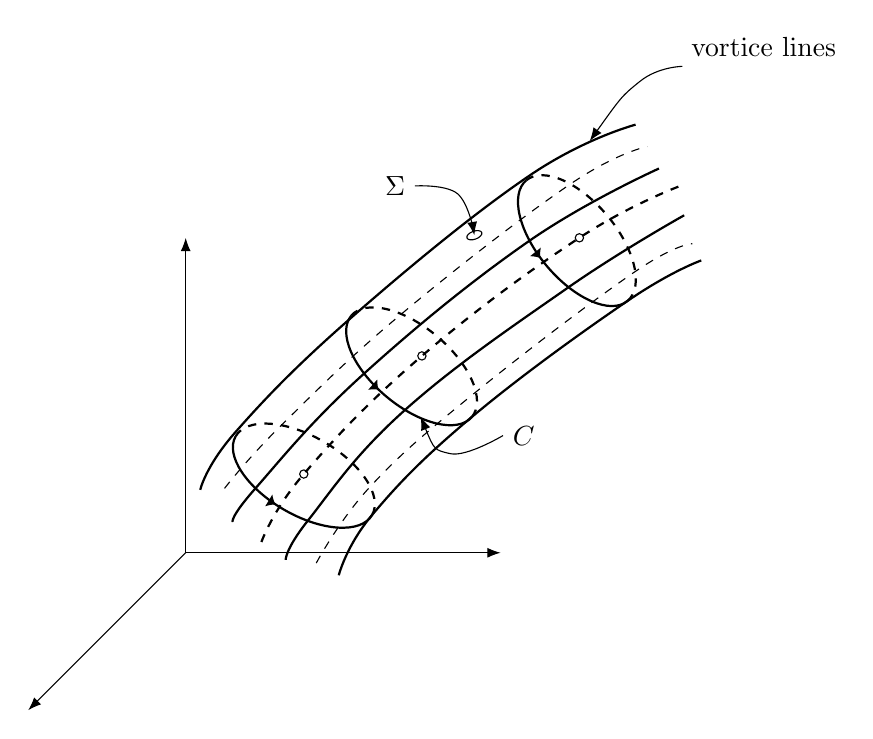
\begin{tikzpicture}
\coordinate (O) at (-15,-5) ;
\coordinate (X) at (-17,-7) ;
\coordinate (Y) at (-11,-5) ;
\coordinate (Z) at (-15,-1) ;
\draw[-Latex] (O)--(X);
\draw [-Latex](O)--(Y);
\draw [-Latex](O)--(Z);
\coordinate (p0) at(-14.0384,-4.8633) {}  ;
\coordinate (p1) at (-13.5,-4) {}  ;
\coordinate (p2) at (-12,-2.5) {} {}  ;
\coordinate (p3) at (-10,-1) {}  ;
\coordinate (p4) at (-8.715,-0.3396);


\coordinate (m0) at(-13.056,-5.286)  {}  ;
\coordinate (m1) at(-12.6333,-4.5206) {}  ;
\coordinate (m2) at (-11.3653,-3.2747) {}  {}  ;
\coordinate (m3) at (-9.389,-1.8018) {} {}  ;
\coordinate (m4) at(-8.4523,-1.2877);

\coordinate (q0) at (-14.8152,-4.2007)  {}  ;
\coordinate (q1) at (-14.3697,-3.4696) {}  ;
\coordinate (q2) at (-12.8618,-1.983) {} {}  {}  ;
\coordinate (q3) at (-10.6228,-0.2025)  {}  ;
\coordinate (q4) at(-9.2862,0.4372);

\coordinate(pin) at (-10.97,-3.5114) {} {} {} {} {} {};
\coordinate (pinb) at (-12.09,-0.3411) {} {} {} {} {};

\draw [rotate=-70,black] (-2.9676,-10.9813) node (v1) {}  circle(0.051cm and 0.1cm);
%\draw [rotate=-50,black,thick] (p2) circle(1cm and 0.5cm);
%\draw [rotate=-50,black,thick] (p3) circle(1cm and 0.5cm);
\draw [rotate=-30,black,thick,decoration={markings, mark=at position 0.52 with {\arrow[scale = 0.1]{Latex[length=-20mm]}}},    postaction={decorate}] (m1) arc (0:-180:1 and 0.5);
\draw [rotate=-30,black,thick,dashed] (m1) arc (0:180:1 and 0.5);

\draw [rotate=-40,black,thick,decoration={markings, mark=at position 0.52 with {\arrow[scale = 0.1]{Latex[length=-20mm]}}},    postaction={decorate}] (m2) arc (0:-180:1 and 0.5);
\draw [rotate=-40,black,thick,dashed] (m2) arc (0:180:1 and 0.5);

\draw [rotate=-50,black,thick,decoration={markings, mark=at position 0.52 with {\arrow[scale = 0.1]{Latex[length=-20mm]}}},    postaction={decorate}] (m3) arc (0:-180:1 and 0.5);
\draw [rotate=-50,black,thick,dashed] (m3) arc (0:180:1 and 0.5);


\draw  [fill= white](p1)circle (1.5pt);
\draw  [fill= white](p2)circle (1.5pt);
\draw  [fill= white](p3)circle (1.5pt);

\node[right] at (pin) {$C$};
\node[left] at (pinb) {$\Sigma$};

\draw[dashed][thick]  plot[smooth, tension=.7] coordinates {(p0) (p1) (p2) (p3) (p4)};
\draw[thick] plot[smooth, tension=.7] coordinates { (m0) (m1) (m2) (m3) (m4) };
\draw[thick]  plot[smooth, tension=.7] coordinates { (q0) (q1) (q2) (q3) (q4) };
%\draw[thick]  plot[smooth, tension=.7] coordinates {(-14.5296,-4.5137) (-14.2098,-4.0796) (-12.8161,-2.6517) (-10.7142,-0.9838) (-9.0577,0.01)};
%\draw[thick]  plot[smooth, tension=.7] coordinates {(-13.7071,-5.1648) (-13.3758,-4.6165) (-12.005,-3.3028) (-10.0402,-1.7264) (-8.6122,-0.8467)};
\draw [dashed] plot[smooth, tension=.7] coordinates {(-14.5068,-4.1824) (-13.7871,-3.3828) (-12.2449,-1.9548) (-10.1201,-0.3213) (-9.1377,0.1585)};
\draw[dashed]  plot[smooth, tension=.7] coordinates {(-13.3416,-5.1306) (-12.6562,-4.1596) (-11.331,-2.9715) (-9.3091,-1.4408) (-8.5665,-1.0752)};
\draw [thick] plot[smooth, tension=.7] coordinates {(-14.404,-4.6095) (-14.1184,-4.1868) (-12.7475,-2.736) (-10.6456,-1.0453) (-8.9892,-0.12)};
\draw[thick]  plot[smooth, tension=.7] coordinates {(-13.73,-5.0893) (-13.4444,-4.5866) (-12.2221,-3.193) (-10.1544,-1.6394) (-8.6693,-0.7141)};

\draw [-Latex]  plot[smooth, tension=.7] coordinates {(pinb) (-11.5481,-0.4399) (v1)};
\node (v2) at (-12.0164,-3.2729) {};
\draw [Latex-]  plot[smooth, tension=.7] coordinates {(v2) (-11.6394,-3.7413) (pin)};
\node[right] (v3) at (-8.7036,1.4295) {\text{vortice lines}};
\draw[Latex-]  plot[smooth, tension=.7] coordinates { (-9.8688,0.2293) (-9.2291,0.9883)(-8.6922,1.1775) };

\draw  plot[smooth, tension=.7] coordinates {(p0)};
\end{tikzpicture}
\caption{Vortex line tube }
\label{fig:fig_p2235}
\end{figure}
We have in rectangular Cartesian coordinates
\begin{align}
\textbf{(6.128)}\quad\spatie &\omega_{jk}=\half\left(v_{k,j}-v_{j,k}\right)\\
\textbf{(6.129)}\quad\spatie &\omega_r=\half\epsilon_{rjk}\omega_{jk}
\end{align}
So we can use the Kelvin-Stokes theorem and form
\begin{align}
\oint_{\partial\Sigma_{C^{'}}} {v_rdx^r }-\oint_{\partial\Sigma_{C}} v_rdx^r&= \iint_{\Sigma_{C^{'}}}\epsilon_{rjk}v_{k,j}n^rdS-\iint_{\Sigma_{C}}\epsilon_{rjk}v_{k,j}n^rdS
\end{align}
Obviously, we have on the surface $\Sigma_{\omega}$ of the tube,  $\hat{\omega}\cdot\hat{n}_{\omega}=0$ and thus $\iint_{\Sigma_{\omega}}\omega_rn^rdS=0$.
Expanding the terms under the integral gives (by $(6.129)$ and $(6.128)$)
\begin{align}
\iint_{\Sigma_{\omega}}\omega_rn^rdS&=\frac{1}{4}\iint_{\Sigma_{\omega}}\epsilon_{rjk}\left(v_{k,j}-v_{j,k}\right)n^rdS
\end{align}
As $\iint_{\Sigma_{\omega}}\omega_rn^rdS=0$ we can put 
\begin{align}
\iint_{\Sigma_{\omega}}\omega_rn^rdS&=\frac{1}{2}\iint_{\Sigma_{\omega}}\epsilon_{rjk}v_{k,j}n^rdS-\frac{1}{2}\iint_{\Sigma_{\omega}}\epsilon_{rjk}v_{j,k}n^rdS\\
&=\frac{1}{2}\iint_{\Sigma_{\omega}}\epsilon_{rjk}v_{k,j}n^rdS-\frac{1}{2}\iint_{\Sigma_{\omega}}\epsilon_{rkj}v_{k,j}n^rdS\\
&=\frac{1}{2}\iint_{\Sigma_{\omega}}\epsilon_{rjk}v_{k,j}n^rdS+\frac{1}{2}\iint_{\Sigma_{\omega}}\epsilon_{rjk}v_{k,j}n^rdS\\
&=\iint_{\Sigma_{\omega}}\epsilon_{rjk}v_{k,j}n^rdS\quad\left(=0\right)
\end{align}
Adding $(8)$ in $(3)$ we get 
\begin{align}
\oint_{\partial\Sigma_{C^{'}}} {v_rdx^r }-\oint_{\partial\Sigma_{C}} v_rdx^r&= \iint_{\Sigma_{C^{'}}}\epsilon_{rjk}v_{k,j}n^rdS+\iint_{\Sigma_{C}}\epsilon_{rjk}v_{k,j}n^rdS+\iint_{\Sigma_{\omega}}\epsilon_{rjk}v_{k,j}n^rdS
\end{align}
Note that in the second term of the right expression, we changed the sign of the normal vector $\hat{n}$ as we want the normal vector on the surface point outward of the considered volume.\\
Using Green's theorem:
\begin{align}
\oint_{\partial\Sigma_{C^{'}}} {v_rdx^r }-\oint_{\partial\Sigma_{C}} v_rdx^r&= \iint_{\Sigma_{C^{'}}}\epsilon_{rjk}v_{k,j}n^rdS+\iint_{\Sigma_{C}}\epsilon_{rjk}v_{k,j}n^rdS+\iint_{\Sigma_{\omega}}\epsilon_{rjk}v_{k,j}n^rdS\\
 &= \iiint_V \epsilon_{rjk}v_{k,jr}dV\\
 &=0
\end{align}
where $V$ is the volume enclosed by the surfaces $\Sigma_{C}$, $\Sigma_{C^{'}}$ and $\Sigma_{\omega}$.\\
And get $d\oint_{\partial\Sigma_{t}} v_rdx^r=0$ along  an infinitesimal displacement along the vortex line  giving 
$$\dv{}{s}\oint_{\partial\Sigma_{t}} v_rdx^r=0$$ where $s$ is a parameter upon which a vortex line can be expressed. \\
Hence $\oint_{\partial\Sigma_{t}} v_rdx^r$ is constant along a vortex line.

 $$\blacklozenge$$
\newpage



\section{p235 - Exercise 5}
\begin{tcolorbox}
Prove that for the type of fluid described in Exercise 2, the vorticity tensor satisfies the differential equations
$$\dv{}{t}\omega_{rs} = \omega_{pr}v_{p,s} - \omega_{ps}v_{p,r}$$
the coordinates being rectangular Cartesians. Write these equations for curvilinear coordinates.\\
Deduce from these equations that, if $\omega_{rs}=0$ initially at some point $P$ in the fluid, these quantities will remain zero permanently for the particle which was initially at $P$.
\end{tcolorbox}
Let's first write down some useful expressions:\\\\
We have in rectangular Cartesian coordinates
\begin{align}
\textbf{(6.128)}\quad\spatie &\omega_{jk}=\half\left(v_{k,j}-v_{j,k}\right)\\
\textbf{(6.129)}\quad\spatie &\omega_r=\half\epsilon_{rjk}\omega_{jk}\\
\Rightarrow\spatie \omega_r&=\half\half\epsilon_{rjk}\left(v_{k,j}-v_{j,k}\right)\\
&=\half\half\epsilon_{rjk}v_{k,j}-\half\half\epsilon_{rjk}v_{j,k}\\
&=\half\half\epsilon_{rjk}v_{k,j}+\half\half\epsilon_{rjk}v_{k,j}\\
&=\half\epsilon_{rjk}v_{k,j}\\
\Rightarrow\spatie \omega_{r,r}&=\half\epsilon_{rjk}v_{k,jr}\\
&=0
\end{align}
So we have, as the flow is steady
\begin{align}
\dv{}{t}\omega_{rs}&= \omega_{rs,p}v_p\\
\text{(1):}\spatie &= \half \left(v_{s,rp}-v_{r,sp}\right)v_p
\end{align}

We have also
\begin{align}
\textbf{(6.146)}\spatie \partial_t v_r +v_sv_{r,s} &= X_r - \rho^{-1}p_{,r}
\end{align}
In the fluid considered here ($\partial_t v_r=0$; $\rho=\rho(p)\Rightarrow \rho^{-1}p_{,r}\coloneqq P_{,r}$; $X_r= -U_{,r}$) and  get
\begin{align}
 v_sv_{r,s} + U_{,r} + P_{,r}=0
\end{align}\\\\
We are now able to deduce the asked expression.\\\\

Consider the following expression $\epsilon_{nmr}\epsilon_{nst}v_mv_{t,s}$. This can be expressed as 
\begin{align}
\epsilon_{nrm}\epsilon_{nst}v_mv_{t,s}&=\left(\delta_{rs}\delta_{mt}-\delta_{rt}\delta_{ms}\right)v_mv_{t,s}\\
&=v_mv_{m,r}-v_mv_{r,m}
\end{align}

giving
\begin{align}
v_sv_{r,s}&= v_sv_{s,r}-\epsilon_{nrm}\epsilon_{nst}v_mv_{t,s}
\end{align}
So (12) can be expressed as 
\begin{align}
&v_sv_{s,r}-\epsilon_{nrm}\epsilon_{nst}v_mv_{t,s} + U_{,r} + P_{,r}=0\\
\text{(6)}\quad\Rightarrow\spatie &v_sv_{s,r}-2\epsilon_{nrm}\omega_nv_m + U_{,r} + P_{,r}=0\\
&v_sv_{s,r}+2\epsilon_{rnm}\omega_nv_m + U_{,r} + P_{,r}=0
\end{align}
Let's take the curl of $(18)$:
\begin{align}
&\epsilon_{pkr}\left(v_sv_{s,r}\right)_{,k}+2\epsilon_{pkr}\epsilon_{rnm}\left(\omega_nv_m\right)_{,k} + \epsilon_{pkr}U_{,rk} + \epsilon_{pkr}P_{,rk}=0
\end{align}
The terms with $U$ and $P$ are of the kind $\nabla\times\nabla(G)$ with $G$ a scalar function $G:\mathbb{R}^3\rightarrow \mathbb{R}$. These terms are equal to zero.\\ 
So, $(19)$ becomes 
\begin{align}
&\underbrace{\epsilon_{pkr}v_{s,k}v_{s,r}}_{=0}+\underbrace{\epsilon_{pkr}v_sv_{s,kr}}_{=0}+2\epsilon_{pkr}\epsilon_{rnm}\left(\omega_nv_m\right)_{,k} =0
\end{align}
Noting that, 
\begin{align}
\epsilon_{pkr}\epsilon_{rnm}\left(\omega_nv_m\right)_{,k} 
&=\epsilon_{rpk}\epsilon_{rnm}\left(\omega_nv_m\right)_{,k}\\
&=\delta_{pn}\delta_{km}\left(\omega_nv_m\right)_{,k}-\delta_{pm}\delta_{kn}\left(\omega_nv_m\right)_{,k}\\
&=\left(\omega_pv_k\right)_{,k}-\left(\omega_kv_p\right)_{,k}\\
&=\omega_{p,k}v_k+\omega_pv_{k,k}-\omega_{k,k}v_p-\omega_kv_{p,k}
\end{align}

Note that the divergence of the vorticity is zero, see $(8)$, so 
\begin{align}
 \epsilon_{pkr}\epsilon_{rnm}\left(\omega_n v_m\right)_{,k}
&= \omega_{p,k}v_k+\omega_pv_{k,k}-\omega_kv_{p,k}
\end{align}
$(25)$ in $(20)$ gives 
\begin{align}
&\omega_{p,k}v_k+\omega_pv_{k,k}-\omega_kv_{p,k} =0
\end{align}
We have $\text{(6): } \omega_p=\half\epsilon_{pmn}v_{n,m},\quad \omega_k=\half\epsilon_{kmn}v_{n,m}$
 giving for $(26)$:
\begin{align}
\epsilon_{pmn}v_{n,mk}v_k+\epsilon_{pmn}v_{n,m}v_{k,k}-\epsilon_{kmn}v_{n,m}v_{p,k} =0
\end{align}
this can also be expressed as 
\begin{align}
\epsilon_{pnm}v_{m,nk}v_k+\epsilon_{pnm}v_{m,n}v_{k,k}-\epsilon_{knm}v_{m,n}v_{p,k} =0
\end{align}
adding $(27)$ and $(28)$ gives 
\begin{align}
&\epsilon_{pnm}\left(v_{m,nk}-v_{n,mk}\right)v_k+\epsilon_{pnm}\left(v_{m,n}-v_{n,m}\right)v_{k,k}-\epsilon_{knm}\left(v_{m,n}-v_{n,m}\right)v_{p,k} =0
\end{align}

\begin{align}
\text{(1),(10):}\quad &\epsilon_{pmn}\dv{\omega_{mn}}{t}+\epsilon_{pmn}\omega_{mn}v_{k,k}-\epsilon_{kmn}\omega_{mn}v_{p,k} =0\\
\times \epsilon_{prs}\quad\Rightarrow\quad &\left(\delta_{rm}\delta_{sn}-\delta_{rn}\delta_{ms}\right)\dv{\omega_{mn}}{t}+\left(\delta_{rm}\delta_{sn}-\delta_{rn}\delta_{ms}\right)\omega_{mn}v_{k,k}-\epsilon_{kmn}\omega_{mn}\epsilon_{prs}v_{p,k} =0\\
\Rightarrow\quad &\dv{\omega_{rs}}{t}-\dv{\omega_{sr}}{t}+\left(\omega_{rs}-\omega_{sr}\right)v_{k,k}-\epsilon_{kmn}\omega_{mn}\epsilon_{prs}v_{p,k} =0
\end{align}
and as $\omega_{rs}$ is skew-symmetric
\begin{align}
\dv{\omega_{rs}}{t}+\omega_{rs}v_{k,k}-\half\epsilon_{kmn}\omega_{mn}\epsilon_{prs}v_{p,k} =0
\end{align}
Let's look at the term $\epsilon_{kmn}\omega_{mn}\epsilon_{prs}v_{p,k} $\\
Suppose $k=p$; then in order to have the term in $\epsilon_{(p)mn}\epsilon_{(p)rs}$ not equal to zero we need
 $$\left(m=r \wedge n=s\right) \vee \left(m=s  \wedge  n=r \right)\quad \text{with } r\neq s$$

and get 
\begin{align}
\half\sum_{(p)}\epsilon_{(p)mn}\omega_{mn}\epsilon_{(p)rs}v_{(p),(p)}&= \half\sum_{(p)}\epsilon_{(p)rs}\omega_{mn}\epsilon_{(p)rs}v_{(p),(p)}\\
&= \half\sum_{(p)}\left(\underbrace{\delta_{(p)(p)}}_{=1}\underbrace{\delta_{ss}}_{=2} -\underbrace{\delta_{(p)s}}_{=0}\delta_{(p)s}\right) \omega_{mn}v_{(p),(p)}\\
&= \sum_{(p)}\omega_{rs}v_{(p),(p)} =\omega_{rs}v_{k,k} 
\end{align}
($\delta_{ss}=2$ as $s$ can not take the value of $(p)$ and so can only span two dimensions.)\\
Hence, the term $\omega_{rs}v_{k,k}$ in $(33)$ vanishes.\\\\

Suppose now that $k\ne p$. We rewrite $\half\epsilon_{kmn}\omega_{mn}\epsilon_{prs}v_{p,k}$ as 

\begin{align}
\half\sum_{(p)}^{p\neq k}\sum_{(k)}^{k\neq p}\epsilon_{(k)mn}\omega_{mn}\epsilon_{(p)rs}v_{(p),(k)} 
\end{align}
noting that the explicit summation symbol only span two dimensions.\\
In $(37)$ as $k\ne p$ we need that $m=p$ or $n= p$ and rewrite $(37)$ as
\begin{align}
\half\sum_{(p)}^{p\neq k}\sum_{(k)}^{k\neq p}\epsilon_{(k)mn}\omega_{mn}\epsilon_{(p)rs}v_{(p),(k)} =&\left\{\begin{array}{l}\quad\half\sum_{(p)}\sum_{(k)}\epsilon_{(k)(p)n}\omega_{(p)n}\epsilon_{(p)rs}v_{(p),(k)} \\\\
+\half\sum_{(p)}\sum_{(k)}\epsilon_{(k)m(p)}\omega_{m(p)}\epsilon_{(p)rs}v_{(p),(k)} \end{array}\right.\\
=&\left\{\begin{array}{l}\quad\half\sum_{(p)}\sum_{(k)}\epsilon_{(p)n(k)}\epsilon_{(p)rs}\omega_{(p)n}v_{(p),(k)} \\\\
+\half\sum_{(p)}\sum_{(k)}\epsilon_{(p)m (k)}\epsilon_{(p)rs}\omega_{(p)m}v_{(p),(k)} \end{array}\right.
\\=&\left\{\begin{array}{l}\quad \half\sum_{(p)}\sum_{(k)}\left(\delta_{nr}\delta_{(k)s}-\delta_{ns}\delta_{(k)r}\right)\omega_{(p)n}v_{(p),(k)} \\\\
+\half\sum_{(p)}\sum_{(k)}\left(\delta_{mr}\delta_{(k)s}-\delta_{(k)r}\delta_{ms}\right)\omega_{(p)m}v_{(p),(k)} 
\end{array}\right.
\\= &\sum_{(p)}\omega_{(p)r}v_{(p),s} - \sum_{(p)}\omega_{(p)s}v_{(p),r}
\end{align}
$(41)$ can now again be written as $\omega_{pr}v_{p,s} - \omega_{ps}v_{p,r}$ (this is possible because, although $p$ only spans two dimensions, the skew-symmetricity of $\omega_{ps}$ permits us to expand $(p)$ to the three dimensions.)\\
Hence, $(33)$ becomes 
$$\dv{\omega_{rs}}{t}-\left( \omega_{pr}v_{p,s} - \omega_{ps}v_{p,r}\right)=0$$
which is the expected expression.
$$\lozenge$$\\
In curvilinear coordinates the expression becomes
$$\fdv{\omega_{rs}}{t}= \omega_{pr}v_{p|s} - \omega_{ps}v_{p|r}$$\\
$$\lozenge$$\\
Suppose that initially at a certain point $\omega_{rs}=0$, then obviously $\fdv{\omega_{rs}}{t}= \omega_{pr}v_{p|s} - \omega_{ps}v_{p|r}=0$ and thus $\omega_{rs} =C$, a constant, which must be zero as the initial condition was that $\omega_{rs}(t=0)=0$.

 $$\blacklozenge$$
\newpage


\section{p236 - Exercise 6}
\begin{tcolorbox}
By eliminating the three components of displacement $u_r$ from the six equations $\mathbf{6.210}$, obtain the following Cartesian equations of compatibility 
$$ e_{rs,mn}+e_{mn,rs}-e_{rm,sn}-e_{sn,rm}=0$$
Show that there are only six independent equations here. Write the equations of compatibility in general tensor form.
\end{tcolorbox}
We have $\mathbf{6.210}$
\begin{align}
e_{rs}= \half\left(u_{r,s}+u_{s,r}\right)
\end{align}
and thus
\begin{align}
\begin{array}{ll}
(a)&e_{rs,mn}= \half\left(u_{r,smn}+u_{s,rmn}\right)\\\\
(b)&e_{mn,rs}= \half\left(u_{m,nrs}+u_{n,mrs}\right)\\\\
(c)&e_{rm,sn}= \half\left(u_{r,msn}+u_{m,rsn}\right)\\\\
(d)&e_{sn,rm}= \half\left(u_{s,nrm}+u_{n,srm}\right)\\\\
\end{array}
\end{align}
giving $e_{rs,mn}+e_{mn,rs}-e_{rm,sn}-e_{sn,rm}= (a)+(b)-(c)-(d)=0$
$$\lozenge$$
Consider the set $(rs)$. Considering the symmetries induced by the symmetry of $e_{rs}$, the number of possible combinations is one of type "repeated combination", i.e.   $\left(\begin{matrix}n+m-1\\m\end{matrix}\right)=\frac{4!}{2!} = 6$. The same is true for the  set $(mn)$, so the total of possible combinations is $36$. But we notice that half of the combinations make the equation indiscernible of the other half; indeed when $(mn)=(rs)$, $e_{rs,mn}+e_{mn,rs}-e_{rm,sn}-e_{sn,rm}=e_{mn,rs}+e_{rs,mn}-e_{mr,ns}-e_{ns,mr}=0$. This reduces the number of combinations to $\frac{36}{2}= 18$.\\
We notice that this is not the total possible number of independent equations yet, as some combinations make the identity trivial. Indeed, consider the case $m=s$. In this case the equation $e_{rs,(s)n}+e_{(s)n,rs}-e_{r(s),sn}-e_{sn,r(s)}=0$ is trivial. The same is true for $n=r$, but also for $m=r$ and $n=s$. Indeed changing $(rs) $ to  $(sr)$ (which is allowed as $e_{rs}$ is symmetric) in  $e_{rs,mn}+e_{mn,rs}-e_{rm,sn}-e_{sn,rm}=0$ we get  $e_{rs,mn}+e_{mn,rs}-e_{sm,rn}-e_{rn,sm}=0$. This expression becomes also trivial when $n=s$ or $m=r$. So the number of independent equations reduces by the number of equations for which yield $ m=r\vee m=s\vee n= r \vee n=s$. This number is $4\times 3=12$ (4 independent events with $3$ possible outcome, each). \\\\
\textbf{So the total of independent equations is $18-12= 6$.}

$$\lozenge$$
In general coordinate system we get, 
$$ e_{rs|mn}+e_{mn|rs}-e_{rm|sn}-e_{sn|rm}=0$$
$$\blacklozenge$$
\newpage



\section{p236 - Exercise 7}
\begin{tcolorbox}
For a rectangular Cartesian coordinates $z_r$, a state of simple tension is represented as $E_{11}=C$ (a constant), all the other components of stress being zero. Find all six covariant components of stress for spherical polar coordinates. 
\end{tcolorbox}
We have $\mathbf{6.223}:$ $T_r=E_{rs}n_s$ so in rectangular Cartesian coordinates we have
\begin{align}
T_1= Cn_1 \quad T_2=0\quad T_3=0
\end{align}
In general we have when going from the rectangular Cartesian coordinates to a curvilinear coordinate system
\begin{align}
T^{'}_r&= T_1x^1_{\ ,'r} \\
T^{'}_r&=E^{'}_{rs}n^{'}_s\\
n^{'s}&= n^{i}x^{'s}_{\ ,i}\\
n^{1}&= n^{'s}x^{1}_{\ ,'s}
\end{align}
Putting this all together we can state
\begin{align}
&E^{'}_{rs}n^{'s}= Cn_1x^{1}_{\ ,'r}\\
\spatie &E^{'}_{rs}n^{'s}= Cn^{'s}x^{1}_{\ ,'s}x^{1}_{\ ,'r}
\end{align}
From which we deduce
\begin{align}
E^{'}_{uv}=Cx^{1}_{\ ,'v}x^{1}_{\ ,'u}
\end{align}
For spherical polar coordinates we have
\begin{align}
\left\{\begin{array}{l}
x^1= r\sin\theta\cos\phi\\
x^1_{,r}= \sin\theta\cos\phi\\
x^1_{,\theta}= r\cos\theta\cos\phi\\
x^1_{,\phi}= -r\sin\theta\sin\phi\\
\end{array}\right.
\end{align}
giving for $(8)$
\begin{align}
\left\{\begin{array}{l}
E_{rr}= C\sin^2\theta\cos^2\phi\\
E_{\theta\theta}= Cr^2\cos^2\theta\cos^2\phi\\
E_{\phi\phi}= Cr^2\sin^2\theta\sin^2\phi\\
E_{r\phi}= Cr\sin\theta\cos\theta\cos^2\phi
\\E_{r\phi}= C\sin^2\theta\cos\phi\sin\phi\\
E_{\theta\phi}= -Cr^2\cos\theta\sin\theta\cos\phi\sin\phi\\
\end{array}\right.
\end{align}
$$\blacklozenge$$
\newpage



\section{p236 - Exercise 8 $\dagger$}
\begin{tcolorbox}
By substitution from $\mathbf{6.247}$ in the Cartesian equations of compatibility  in Exercise 6, deduce that in a homogeneous isotropic body in equilibrium under body forces $X_r$, the invariant $\Theta= E_{nn}$ satisfies the following partial differential equation:
$$\left(1-\sigma\right)\Theta_{,rr}= \left(1+\sigma\right)\rho X_{r,r}$$
\end{tcolorbox}
Let's recap what we know
\begin{align}
\begin{array}{lll}
(a)&e_{rs,mn}+e_{mn,rs}-e_{rm,sn}-e_{sn,rm}=0&\text{(Exercise 6)}\\\\
(b)&e_{rs}= \frac{1}{E}\left[\left(1+\sigma\right)E_{rs}-\sigma \delta_{rs} E_{nn}\right]&\text{(6.247)}\\\\
(c)&E=\frac{\mu\left(3\lambda+2\mu\right)}{\lambda+\mu}, \quad\sigma= \frac{\lambda}{2\left(\lambda+\mu\right)}&\text{(6.248)}\\\\
(d)&\lambda=\frac{\sigma E}{\left(1+\sigma\right)\left(1-2\sigma\right)}, \quad\mu =\frac{E}{2\left(1+\sigma\right)}&\text{(6.249)}\\\\
(e)&\rho f_r=\rho X_r +\left(\lambda+\mu\right)\theta_{,r}+\mu\Delta u_r&\text{(6.250)}\\\\
(f)&\theta = e_{nn}&\text{(6.246)}\\\\
(g)&e_{rs}=\half\left(u_{r,s}+u_{s,r} \right)&\text{(6.210)}
\end{array}
\end{align}
As we are in steady state we have  $ f_r=\pdv[2]{u_r}{t}=0$ and $(e)$ becomes
\begin{align}
&\rho X_r +\left(\lambda+\mu\right)\theta_{,r}+\mu\Delta u_r=0\\
\Rightarrow\quad &\rho X_{r,r} +\left(\lambda+\mu\right)\theta_{,rr}+\mu\left(\Delta u_r\right)_{,r}=0
\end{align}
Put $m=n$ and $s=r$ in $(a)$:
\begin{align}
&\underbrace{e_{rr,nn}}_{=\theta_{,nn}}+\underbrace{e_{nn,rr}}_{=\theta_{,nn}}-e_{rn,rn}-e_{rn,rn}=0\\
\text{or}\quad & \theta_{,nn}=e_{nr,nr} 
\end{align}
Putting $(b)$ in $(5)$ we get
\begin{align}
\theta_{,rr}&= \frac{1}{E}\left[\left(1+\sigma\right)E_{nr,nr}-\sigma\delta_{nr}E_{kk,nr}\right]\\
&= \frac{1}{E}\left[\left(1+\sigma\right)E_{nr,nr}-\sigma E_{kk,rr}\right]\\
&= \frac{1}{E}\left(1+\sigma\right)E_{nr,nr}- \frac{\sigma}{E} E_{kk,rr}
\end{align}
Put $\Theta=E_{kk}$, then 
\begin{align}
\theta_{,rr}&= \frac{1}{E}\left(1+\sigma\right)E_{nr,nr}- \frac{\sigma}{E} \Theta_{,rr}
\end{align}
Consider now $\Delta u_r = u_{r,kk}$, using $e_{rs}=\half\left(u_{r,s}+u_{s,r} \right)$ we have 
\begin{align}
e_{rs,rs}&= \half\left(u_{r,srs}+u_{s,rrs} \right)\\
&=u_{r,ssr}
\end{align}
but $ u_{r,ss}=\Delta u_r$, then
\begin{align}
\left(\Delta u_r\right)_{,r}&= e_{rs,rs} 
\end{align} 
So, by $(5)$,
\begin{align}
\left(\Delta u_r\right)_{,r}&=\theta_{,rr}
\end{align}
Let's recap what we already know.
We have $(3)$ and $(13)$ 
\begin{align}
\left\{\begin{array}{ll}
(3)&\rho X_{r,r} +\left(\lambda+\mu\right)\theta_{,rr}+\mu\Delta \left(u_r\right)_{,r}=0\\\\
(13)&\left(\Delta u_r\right)_{,r}=\theta_{,rr}
\end{array}\right.
\end{align}
and also 
\begin{align}
\left(1+\sigma\right)E_{nr,nr} = \left(1-\sigma\right)\Theta_{,rr}
\end{align}
indeed $(a)$ gives
\begin{align}
&e_{rn,rn} = e_{rr,ss}\\
\Rightarrow \quad & \frac{1}{E}\left[\left(1+\sigma\right)E_{rn,rn}-\sigma \delta_{rn}E_{kk,rn}\right]= \frac{1}{E}\left[\left(1+\sigma\right)E_{rr,ss}-\sigma \delta_{rr}E_{kk,ss}\right]\\
\Leftrightarrow\quad & \left(1+\sigma\right)E_{rn,rn}-\sigma \Theta_{,rr}= \left(1+\sigma\right)\Theta_{,rr}-\sigma 3\Theta_{,rr}\\
\Leftrightarrow\quad & \left(1+\sigma\right)E_{rn,rn}= \left(1-\sigma\right)\Theta_{,rr}
\end{align}
So, $(9)$ becomes
\begin{align}
\theta_{,rr}&= \frac{1}{E}\left(1+\sigma\right)E_{rn,rn}- \frac{\sigma}{E} \Theta_{,rr} \\
&=\frac{1-2\sigma}{E}\Theta_{,rr} 
\end{align}
and  $(14)$ becomes
\begin{align}
\left(\Delta u_r\right)_{,r}=\frac{1-2\sigma}{E}\Theta_{,rr} 
\end{align}
Let's put $\xi= \left(\lambda+\mu\right)\theta_{,rr}+\mu\left(\Delta u_r\right)_{,r}$ with $(22)$ and $(23)$ we get
\begin{align}
\xi &= \left[\left(\lambda+\mu\right)\frac{1-2\sigma}{E}+\mu \frac{1-2\sigma}{E}\right]\Theta_{,rr} \\
&= \frac{1-2\sigma}{E}\left(\lambda+2\mu\right)\Theta_{,rr}
\end{align}
Using $(d)$ in this expression gives 
\begin{align}
\xi&= \frac{1-2\sigma}{E}E\left(\frac{\sigma}{\left(1+\sigma\right)\left(1-2\sigma\right)}+ \frac{1}{\left(1+\sigma\right)}\right)\Theta_{,rr}\\
&= \left(1-2\sigma\right)\frac{\sigma+\left(1-2\sigma\right)}{\left(1+\sigma\right)\left(1-2\sigma\right)}\Theta_{,rr}\\
&= \frac{1-\sigma}{1+\sigma}\Theta_{,rr}
\end{align}
giving for $(3$)
$$\left(1+\sigma\right)\rho X_{r,r} \underbrace{+}_{?\text{ should be } -}\left(1-\sigma \right)\Theta_{,rr}=0$$
$$\blacklozenge$$
\newpage




\section{p236 - Exercise 9}
\begin{tcolorbox}
In a state of plane stress we have $E_{\alpha 3}=0,E_{3 3}=0$, the coordinates being Cartesian, and Greek suffixes taking the values $1,\ 2$. prove that the equations of equilibrium under no body forces are satisfied if we put
$$E_{\alpha \beta} = \epsilon_{\alpha\rho}\epsilon_{\beta \sigma} \psi_{,\rho \sigma} $$
where $\psi$ is an arbitrary function. Show that this gives $$E_{11}=\psi_{,22}, \quad E_{12}=-\psi_{,12},\quad E_{22}=\psi_{,11},$$
\end{tcolorbox}
Given that we are in equilibrium and no body forces acting we have from $\rho f_r=\rho X_r +E_{rs,s}$ w have
\begin{align}
E_{rs,s}=0
\end{align}
Explicitly
\begin{align}
E_{rs,s}=E_{r1,1}+E_{r2,2}+\underbrace{E_{r3,3}}_{=0}
\end{align}
and for $r=3$
\begin{align}
E_{3s,s}=\underbrace{E_{31,1}}_{=0}+\underbrace{E_{32,2}}_{=0}+\underbrace{E_{33,3}}_{=0}
\end{align}
So $(1)$ can be expressed as 
\begin{align}
E_{\alpha\beta,\beta}=0
\end{align}
Let's test the expression $E_{\alpha \beta} = \epsilon_{\alpha\rho}\epsilon_{\beta \sigma} \psi_{,\rho \sigma} $
\begin{align}
E_{\alpha \beta,\beta} &= \epsilon_{\alpha\rho}\epsilon_{\beta \sigma} \psi_{,\rho \sigma\beta}\\
&= 0
\end{align}
The last identity is due to the fact that for a fixed $\alpha$,\\ or $\rho$ will take the value of $\alpha$ (making $\epsilon_{\alpha\rho}=0$), \\or for $\rho\ne\alpha$, the only non-zero terms imply that $\beta\ne\sigma$ where the expansion is of the form $\epsilon_{\alpha\rho}\epsilon_{\alpha\rho} \psi_{,\rho \sigma\beta}+\epsilon_{\alpha\rho}\epsilon_{\rho\alpha} \psi_{,\rho \sigma\beta}$ (no summation over dummy indexes) and as the order of partial differentiation is of no importance and $\epsilon_{\rho\alpha}$ and $\epsilon_{\alpha\rho}$ are of opposite sign, the two terms will cancel each other.\\
So indeed, $E_{\alpha \beta} = \epsilon_{\alpha\rho}\epsilon_{\beta \sigma} \psi_{,\rho \sigma} $ satisfies the differential equation $E_{rs,s}=0$.
$$\lozenge$$
Let's calculate explicitly the $E_{\alpha\beta}$.\\
$\epsilon_{\alpha\rho}\ne0$ implies $\alpha\ne\rho$ and $\epsilon_{\beta \sigma}\ne0$ implies $\beta \ne\sigma$, hence
\begin{align*}
\begin{array}{ll}
E_{11}&=\epsilon_{12}\epsilon_{12}\psi_{,22}\\
&=(1)(1)\psi_{,22}\\
&=\psi_{,22}\\\\
E_{22}&=\epsilon_{21}\epsilon_{21}\psi_{,11}\\
&=(-1)(-1)\psi_{,11}\\
&=\psi_{,11}\\\\
E_{12}&=\epsilon_{12}\epsilon_{21}\psi_{,21}\\
&=(1)(-1)\psi_{,21}\\
&=-\psi_{,21}
\end{array}
\end{align*}
$$\blacklozenge$$
\newpage


\section{p236 - Exercise 10}
\begin{tcolorbox}
An isotropic elastic body is in equilibrium under no body forces. show that, for rectangular Cartesian coordinates, the displacement satisfies the partial differential equations
$$\left(1-2\sigma\right)\Delta u_r+\theta_{,r}=0$$
Deduce that $\theta$ is a harmonic function.\\
Show that the above equations are satisfied if we put 
$$u_r=\psi_r-\frac{1}{4\left(1-\sigma\right)}\left(z_s\psi_s+\phi\right)_{,r}$$
provided $\Delta\phi=0$, $\Delta\psi_r=0$. (Papcovich-Neuber)
\end{tcolorbox}
As we are in equilibrium (no acceleration) and no body forces, equation $$\mathbf{6.250}\quad \rho f_r = \rho X_r + \left(\lambda+\mu\right)\theta_{,r} + \mu\Delta u_r$$ becomes
\begin{align}
\left(\lambda+\mu\right)\theta_{,r} + \mu\Delta u_r = 0
\end{align}
with 
\begin{align}
\lambda= \frac{\sigma E}{\left(1+\sigma\right)\left(1-2\sigma\right)}, \quad \mu= \frac{ E}{2\left(1+\sigma\right)}
\end{align}
so $(1)$ becomes 
\begin{align}
&\frac{E}{\left(1+\sigma\right)}\left(\frac{\sigma }{1-2\sigma}+\half\right)\theta_{,r} + \frac{ E}{2\left(1+\sigma\right)}\Delta u_r = 0\\
\Leftrightarrow\quad & \left(\frac{2\sigma +1-2\sigma}{2\left(1-2\sigma\right)}\right)\theta_{,r}+\half\Delta u_r = 0\\
\Leftrightarrow\quad & \theta_{,r}+\left(1-2\sigma\right)\Delta u_r = 0
\end{align}
$$\lozenge$$
We show now that $\theta$ is an harmonic function .
\begin{align}
(5)_{,r}\quad\Rightarrow\quad & \theta_{,rr}+\left(1-2\sigma\right)\left(\Delta u_r\right)_{,r} = 0\\
\Rightarrow\quad &\Delta \theta+\left(1-2\sigma\right)\left(\Delta u_r\right)_{,r} = 0
\end{align}
We have 
\begin{align}
&\Delta u_r = u_{r,ss}\\
\Rightarrow\quad & \left(\Delta u_r\right)_{,r} = u_{r,rss}
\end{align}
and from exercise 8 $(11),\ (12),\ (13)$ we know 
\begin{align}
&\left(\Delta u_r\right)_{,r}=\theta_{rr}=\Delta \theta
\end{align}
and $(7)$ becomes
\begin{align}
&\Delta \theta+\left(1-2\sigma\right)\Delta \theta = 0\\
\Rightarrow\quad & \Delta \theta=0
\end{align}
$\theta$ is an harmonic function.
$$\lozenge$$
\begin{align}
u_r&=\psi_r-\frac{1}{4\left(1-\sigma\right)}\left(z_s\psi_s+\phi\right)_{,r}\\
\Rightarrow\quad \Delta u_r&=\underbrace{\Delta \psi_r}_{=0}-\frac{1}{4\left(1-\sigma\right)}\Delta \left(z_s\psi_s+ \phi\right)_{,r}\\
&=-\frac{1}{4\left(1-\sigma\right)} \left(z_s\psi_s+  \phi\right)_{,rkk}\\
&=-\frac{1}{4\left(1-\sigma\right)} \left[\left(z_{s,r}\psi_s+z_s\psi_{s,r}\right)_{,kk}+ \underbrace{\phi_{,rkk}}_{\left(\Delta\phi\right)_r=0}\right]\\
&=-\frac{1}{4\left(1-\sigma\right)} \left(\delta_{sr}\psi_s+z_s\psi_{s,r}\right)_{,kk}\\
&=-\frac{1}{4\left(1-\sigma\right)} \left(\psi_r+z_s\psi_{s,r}\right)_{,kk}\\
&=-\frac{1}{4\left(1-\sigma\right)} \left(\underbrace{\psi_{r,kk}}_{=0}+\left(\underbrace{z_{s,k}}_{= \delta_{sk}}\psi_{s,r}+z_s\psi_{s,rk}\right)_{,k}\right)\\
&=-\frac{1}{4\left(1-\sigma\right)} \left(\psi_{k,rk}+z_{s,k}\psi_{s,rk}+z_s\underbrace{\psi_{s,rkk}}_{=0}\right)\\
&=-\frac{1}{4\left(1-\sigma\right)} \left(\psi_{k,rk}+\psi_{k,rk}\right)\\
\Rightarrow\quad \Delta u_r&=-\frac{1}{2\left(1-\sigma\right)} \psi_{k,kr}
\end{align}
Let's look at $\theta=e_{nn}$. As $e_{rs}=\half\left(u_{r,s}+u_{s,r}\right)$
\begin{align}
\theta &= u_{k,k}\\
&= \left(\psi_k-\frac{1}{4\left(1-\sigma\right)}\left(z_s\psi_s+\phi\right)_{,k}\right)_{,k}\\
&= \psi_{k,k}-\frac{1}{4\left(1-\sigma\right)}\left(\left(z_s\psi_s+\phi\right)_{,k}\right)_{,k}\\
&= \psi_{k,k}-\frac{1}{4\left(1-\sigma\right)}\left(\left(z_{s,k}\psi_s+ z_s\psi_{s,k}\right)_k+\underbrace{\phi_{,kk}}_{=0}\right)\\
&= \psi_{k,k}-\frac{1}{4\left(1-\sigma\right)}\left(\psi_{k,k}+ z_{s,k}\psi_{s,k}+z_s\psi_{s,kk}\right)\\
&= \psi_{k,k}-\frac{1}{4\left(1-\sigma\right)}\left(\psi_{k,k}+ \psi_{k,k}+z_s\underbrace{\psi_{s,kk}}_{=0}\right)\\
&= \psi_{k,k}-\frac{1}{2\left(1-\sigma\right)}\psi_{k,k}\\
\Rightarrow\quad &\theta = \frac{1-2\sigma}{2\left(1-\sigma\right)}\psi_{k,k}\\
\Rightarrow\quad &\theta_{,r} = \frac{1-2\sigma}{2\left(1-\sigma\right)}\psi_{k,kr}
\end{align}
Be $\Gamma= \left(1-2\sigma\right)\Delta u_r+\theta_{,r}$ and let's plug into it $(22)$ and $(31)$
\begin{align}
\Gamma&= \left(1-2\sigma\right)\Delta u_r+\theta_{,r}\\
&= -\left(1-2\sigma\right)\frac{1}{2\left(1-\sigma\right)} \psi_{k,kr}+\frac{1-2\sigma}{2\left(1-\sigma\right)}\psi_{k,kr}\\
&=0
\end{align}
so indeed $$u_r=\psi_r-\frac{1}{4\left(1-\sigma\right)}\left(z_s\psi_s+\phi\right)_{,r}$$ is a solution of $$\left(1-2\sigma\right)\Delta u_r+\theta_{,r}=0$$
$$\blacklozenge$$
\newpage


\section{p237 - Exercise 11}
\begin{tcolorbox}
If, for rectangular Cartesian coordinates $z_r$, $\chi_{rs}$ is any symmetric tensor, show that the tensor $E_{mn}$ defined by
$$E_{mn}= \epsilon_{mpr}\epsilon_{nqs}\chi_{rs,pq}$$
is symmetric, and satisfies the equations $E_{mn,n}= 0$.\\ Show that if we choose $\chi_{rs}= z_rz_s$, then $E_{mn}= -2\delta_{mn}$.
\end{tcolorbox}
\begin{align*}
E_{nm}&= \epsilon_{npr}\epsilon_{mqs}\chi_{rs,pq}\\
&= \epsilon_{npr}\epsilon_{mqs}\chi_{sr,qp}\\
&= \epsilon_{nqs}\epsilon_{mpr}\chi_{rs,pq}\\
&= E_{mn}
\end{align*}
$$\lozenge$$
Consider $$E_{mn,n}= \epsilon_{mpr}\epsilon_{nqs}\chi_{rs,pqn}$$
As $\epsilon_{nqs}$ is antisymmetric in $(n,q)$ and $\chi_{rs,pqn}$ is symmetric in these indices,  $E_{mn,n}$ reduces to a sum of terms of the type $\epsilon_{mpr}\epsilon_{(nq)s}\chi_{rs,p(qn)}-\epsilon_{mpr}\epsilon_{(nq)s}\chi_{rs,p(nq)}$.\\
So, $E_{mn,n}=0$
$$\lozenge$$
Be $\chi_{rs}= z_rz_s$, then
\begin{align*}
E_{mn}&= \epsilon_{mpr}\epsilon_{nqs}(z_rz_s)_{,pq}\\
&= \epsilon_{mpr}\epsilon_{nqs}(\delta_{pr}z_s+\delta_{sp}z_r)_{,q}\\
&= \epsilon_{mpr}\epsilon_{nqs}(\delta_{pr}\delta_{sq}+\delta_{sp}\delta_{rq})\\
&= \underbrace{\epsilon_{mpp}\epsilon_{nqq}}_{=0}+\epsilon_{mpq}\epsilon_{nqp}\\
&= \epsilon_{pmq}\epsilon_{pqn}\\
&= \delta_{mq}\delta_{qn}-\delta_{mn}\underbrace{\delta_{qq}}_{=3}\\
&= \delta_{mn}-3\delta_{mn}\\
&= -2\delta_{mn}
\end{align*}
$$\blacklozenge$$
\newpage


\section{p237 - Exercise 12}
\begin{tcolorbox}
The determinantal equation $\left|\lambda\delta_{mn}-E_{mn}\right|=0$ is important in elasticity because it gives the three principal stresses at a point. Show that if we introduce the three Cartesian invariants
$$A=E_{mn},\quad B=E_{mm}E_{mn}, \quad C= E_{mn}E_{np}E_{pm}$$ the cubic equation ma be written in the form
$$\lambda^3-A\lambda^2-\half\left(A^2-B\right)\lambda-\left(\frac{1}{6}A^3-\half AB+\frac{1}{3}C\right)=0$$
[Hint: Note the Cartesian invariance of this expression, and use coordinates which make $E_{rs}=0$ for $r\neq s$.]
\end{tcolorbox}
Be a matrix $M_{pq}$. It's determinant can be expressed as $\left|M_{pq}\right|= \epsilon_{mnr}M_{1m}M_{2n}M_{3r}$ or - see $\mathbf{(4.316)}$-  $\epsilon_{stu}\left|M_{pq}\right|= \epsilon_{mnr}M_{sm}M_{tn}M_{ur}$ or $\epsilon_{stu}\epsilon_{stu}\left|M_{pq}\right|=6\left|M_{pq}\right|= \epsilon_{stu}\epsilon_{mnr}M_{sm}M_{tn}M_{ur}$.\\\\
Put $$M_{pq}= \lambda\delta_{mn}-E_{mn}$$
and get
\begin{align}
6\left|M_{pq}\right|&= \epsilon_{stu}\epsilon_{mnr}\left(\lambda\delta_{sm}-E_{sm}\right)\left(\lambda\delta_{tn}-E_{tn}\right)\left(\lambda\delta_{ur}-E_{ur}\right)\\
&=\left\{\begin{array}{l}
\epsilon_{stu}\epsilon_{mnr}\left\{\right.\\
\lambda^3\delta_{sm}\delta_{tn}\delta_{ur}\\
-\lambda^2\delta_{sm}\delta_{ur}E_{tn}-\lambda^2\delta_{tn}\delta_{ur}E_{sm}-\lambda^2\delta_{sm}\delta_{tn}E_{ur}\\
+\lambda\delta_{ur}E_{sm}E_{tn}+\lambda\delta_{sm}E_{tn}E_{ur}+\lambda\delta_{tn}E_{sm}E_{ur}\\
-E_{sm}E_{tn}E_{ur}\\
\left.\right\}
\end{array}\right.\\
&=\left\{\begin{array}{l}
\lambda^3\underbrace{\epsilon_{stu}\epsilon_{stu}}_{=6}\\
-\lambda^2\underbrace{\epsilon_{stu}\epsilon_{snu}}_{=2\delta_{tn}}E_{tn}-\lambda^2\underbrace{\epsilon_{stu}\epsilon_{mtu}}_{=2\delta_{sm}}E_{sm}-\lambda^2\underbrace{\epsilon_{stu}\epsilon_{str}}_{=2\delta_{ur}}E_{ur}\\
+\lambda\underbrace{\epsilon_{stu}\epsilon_{mnu}}_{=\delta_{sm}\delta_{tn}-\delta_{sn}\delta_{tm}}E_{sm}E_{tn}+\lambda\underbrace{\epsilon_{stu}\epsilon_{snr}}_{=\delta_{tn}\delta_{ur}-\delta_{tr}\delta_{un}}E_{tn}E_{ur}+\lambda\underbrace{\epsilon_{stu}\epsilon_{mtr}}_{=\delta_{sm}\delta_{ur}-\delta_{sm}\delta_{ur}}E_{sm}E_{ur}\\
-\epsilon_{stu}\epsilon_{mnr}E_{sm}E_{tn}E_{ur}
\end{array}\right.
\end{align}
working out gives 
\begin{align}
6\left|M_{pq}\right|&= 6\lambda^3-6A\lambda^2 +\left(3A^2-3B\right)\lambda-\epsilon_{stu}\epsilon_{mnr}E_{sm}E_{tn}E_{ur}
\end{align}
but the term $\epsilon_{stu}\epsilon_{mnr}E_{sm}E_{tn}E_{ur}=6\left|E_{pq}\right|$
giving 
\begin{align}
\left|M_{pq}\right|&= \lambda^3-A\lambda^2 +\half\left(A^2-B\right)\lambda-\left|E_{pq}\right|
\end{align}
Let's consider now the invariants $$A=E_{mn},\quad B=E_{mm}E_{mn}, \quad C= E_{mn}E_{np}E_{pm}$$
As $(E_{pq})$ is symmetric with  elements $\in \mathbb{R}$, we know that there is an orthogonal transformations so that $(E_{pq})$ becomes diagonal:
\begin{align}
(E_{pq})&= \left(\begin{matrix}
E_1&0&0\\
0&E_2&0\\
0&0&E_3\\
\end{matrix}\right)
\end{align}
The invariants $A, \ B,\ C$ become
\begin{align}
\left\{\begin{array}{l}
A= E_1+E_2+E_3\\
B= E_1^2+E_2^2 +E_3^2\\
A= E_1^3+E_2^3+E_3^3\\
\left|E_{pq}\right|= E_1E_2E_3
\end{array}\right.
\end{align}
We will try to express $\left|E_{pq}\right|$ as an expression of $A, \ B,\ C$. Obviously as $\left|E_{pq}\right|= E_1E_2E_3$ we need at least $A^3$  
\begin{align}
A^3&= \left\{\begin{array}{l}E_1^3+E_2^3+E_3^3\\+3E_1E_2^2+3E_1E_3^2+3E_1^2E_2+3E_1^2E_3+3E_2^2E_3+3E_3^2E_2\\
+ 6E_1E_2E_3
\end{array}\right.\\
&= C+6\left|E_{pq}\right|+3\left(E_1E_2^2+E_1E_3^2+E_1^2E_2+E_1^2E_3+E_2^2E_3+E_3^2E_2\right)
\end{align}
and $AB$
\begin{align}
AB&= \left(E_1+E_2+E_3\right)\left(E_1^2+E_2^2 +E_3^2\right)\\
&= E_1^3+E_2^3 +E_3^3+ E_1E_2^2+E_1E_3^2+E_1^2E_2+E_1^2E_3+E_2^2E_3+E_3^2E_2\\
&= C+ E_1E_2^2+E_1E_3^2+E_1^2E_2+E_1^2E_3+E_2^2E_3+E_3^2E_2
\end{align}
hence 
\begin{align}
A^3-3AB&= C+ 6\left|E_{pq}\right|-3C\\
&= 6\left|E_{pq}\right|-2C\\
\Rightarrow\quad 6\left|E_{pq}\right|&=A^3-3AB+2C
\end{align}
and $(5)$ becomes
\begin{align}
\left|M_{pq}\right|&= \lambda^3-A\lambda^2 +\half\left(A^2-B\right)\lambda-\left(\frac{1}{6}A^3-\half AB+\frac{1}{3}C\right)
\end{align}
Putting $\left|M_{pq}\right|=0$ gives the required equation.
$$\blacklozenge$$
\newpage



\section{p237 - Exercise 13}
\begin{tcolorbox}
A plane electromagnetic wave in complex form is given,
$$E_{\alpha}=A_{\alpha}e^{iS},\quad  E_3=0,\quad H_{\alpha} = -\epsilon_{\alpha\beta}A_{\beta}e^{iS},\quad H_3=0$$ $$ S=\frac{2\pi}{\lambda}\left(z_3-ct\right)$$
where $A_{\alpha}$ is a constant complex vector, and Greek suffixes take the values $1,2$. Verify that Maxwell's equations are satisfied, and that the wave is propagated in the positive $z_3-$direction.\\
The wave meets a perfectly conducting wall $z_3=0$,and is reflected. Given the condition on such wall is that the tangential component of the electric vector for the total field vanishes, show that the reflected wave is given by
$$E^{'}_{\alpha}=-A_{\alpha}e^{iS^{'}},\quad E^{'}_{3}=0, \quad H^{'}_{\alpha} = -\epsilon_{\alpha\beta} A_{\beta}e^{iS^{'}},\quad H^{'}_3=0,$$
$$S^{'}= -\frac{2\pi}{\lambda}\left(z_3+ct\right)$$
\end{tcolorbox}
Maxwell's equations read 
\begin{align}
\left\{\begin{array}{lll}(6.301)& \frac{1}{c}\partial_t E_r=\epsilon_{rmn}H_{n,m}& \frac{1}{c}\partial_t H_r=-\epsilon_{rmn}E_{n,m}\\\\
(6.302)&E_{n,n}=0&H_{n,n}=0
\end{array}\right.
\end{align}
For $\mathbf{(6.302)}$ this gives for the considered case
\begin{align}
E_{n,n}&=E_{\alpha,\alpha}+ \underbrace{E_{3,3}}_{=0}\\
&=A_{\alpha}\left(e^{iS}\right)_{,\alpha}\\
&=iA_{\alpha}e^{iS}\underbrace{S_{,\alpha}}_{=0}\\
&=0
\end{align}
analogously
\begin{align}
H_{n,n}&=H_{\alpha,\alpha}+ \underbrace{H_{3,3}}_{=0}\\
&=-\epsilon_{\alpha\beta}A_{\beta}\left(e^{iS}\right)_{,\alpha}\\
&=-i\epsilon_{\alpha\beta}A_{\beta}\underbrace{S_{,\alpha}}_{=0}\\
&=0
\end{align}
So for $\mathbf{6.302}$ the considered wave meets Maxwell's equations.\\
And for $\mathbf{6.301}$ 
\begin{align}
\frac{1}{c}\partial_t E_{\alpha}&=\epsilon_{\alpha mn}H_{n,m}\\
\epsilon_{\alpha mn}H_{n,m}&= \epsilon_{\alpha\beta\gamma}H_{\gamma,\beta}+\epsilon_{\alpha 3\beta}H_{\beta,3}+\epsilon_{\alpha\beta 3}\underbrace{H_{3,\gamma}}_{=0}\\
&= -i\epsilon_{\alpha\beta\gamma}\epsilon_{\gamma\delta}A_{\delta}e^{iS}\underbrace{S_{,\beta}}_{=0}-i\epsilon_{\alpha 3 \beta}\epsilon_{\beta \gamma}A_{\gamma}e^{iS}\underbrace{S_{,3}}_{=\frac{2\pi}{\lambda}}\\
&= -i\frac{2\pi}{\lambda}\epsilon_{\alpha 3 \beta}\epsilon_{\beta \gamma}A_{\gamma}e^{iS}\\
&= i\frac{2\pi}{\lambda}\epsilon_{\alpha  \beta 3 }\epsilon_{\beta \gamma}A_{\gamma}e^{iS}
\end{align}
Let's look at $(14)$ and more specifically at the factor $\epsilon_{\alpha  \beta 3}$. As the third index is fixed we can replace $\epsilon_{\alpha  \beta  3}$ by $\epsilon_{\alpha  \beta}$ and get 
\begin{align}
\epsilon_{\alpha mn}H_{n,m}&= i\frac{2\pi}{\lambda}\epsilon_{\alpha  \beta  }\epsilon_{\beta \gamma}A_{\gamma}e^{iS}\\
&= -i\frac{2\pi}{\lambda}A_{\alpha}e^{iS}
\end{align}
and 
\begin{align}
\frac{1}{c}\partial_t E_{\alpha}&=\frac{1}{c}iA_{\alpha}e^{iS}\left(-c\frac{2\pi}{\lambda}\right)\\
&=-i\frac{2\pi}{\lambda}A_{\alpha}e^{iS}
\end{align}

So for $\mathbf{6.301 (a)}$ the considered wave meets Maxwell's equations.\\
For the second equation: 
\begin{align}
\frac{1}{c}\partial_t H_{\alpha}&=-\epsilon_{\alpha mn}E_{n,m}\\
\epsilon_{\alpha mn}E_{n,m}&= -\epsilon_{\alpha\beta\gamma}\underbrace{E_{\gamma,\beta}}_{=0}-\epsilon_{\alpha 3\beta}E_{\beta,3}-\epsilon_{\alpha\beta 3}\underbrace{E_{3,\gamma}}_{=0}\\
&=-\epsilon_{\alpha 3\beta}E_{\beta,3}\\
&= -i\frac{2\pi}{\lambda}\epsilon_{\alpha 3\beta}A_{\beta}e^{iS}\\
&= i\frac{2\pi}{\lambda}\epsilon_{\alpha \beta }A_{\beta}e^{iS}\\
\frac{1}{c}\partial_t H_{\alpha}&= i\frac{2\pi}{\lambda}\epsilon_{\alpha \beta}A_{\beta}e^{iS}
\end{align}

So for $\mathbf{6.301 (b)}$ the considered wave meets Maxwell's equations and also for all the other equations in Maxwell's equations set.\\
$$\lozenge$$
As in the equation of the plane the only varying parameter is $S=\frac{2\pi}{\lambda}\left(z_3-ct\right)$  (depending on space and time), the components of $E_r, \quad H_r$ will remain constant only when $S= $ constant and as $S$ is  only spatially dependent of $z_3$ the plane can only move in the $z_3-$direction. Indeed, at a certain configuration point $(z_1,z_2,z_3,t)$ the configuration is the same $\forall z_1,\quad z_2$ for a given pair $(z_3,t)$. At a time $t^{'}$ the value of $E_r,\quad H_r$ will be the same if $z_3-ct= z^{'}_3-ct^{'}$, giving $z^{'}_3=z_3+ c(t^{'}- t)$:  a plane with certain configuration $(z_1,z_2,z_3,t_0)$ will move along the $z_3$ axis with speed $c$
$$\lozenge$$
\begin{figure}[H]%
    \centering
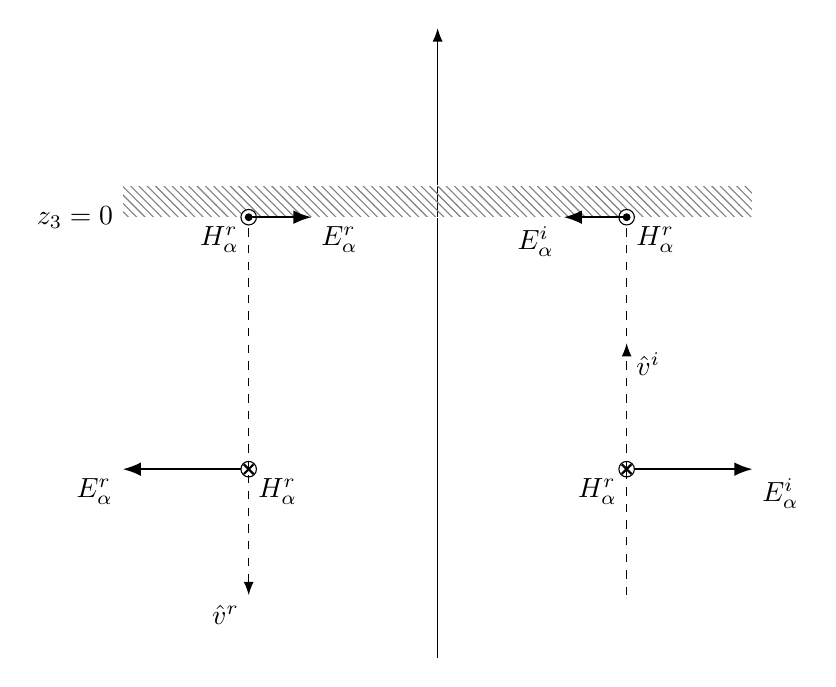
\begin{tikzpicture}[scale=0.8]
\tikzset{cross/.style={cross out, draw=black, minimum size=3.5, inner sep=0pt, outer sep=0pt},
%default radius will be 1pt. 
cross/.default={1pt}}
\coordinate (O) at (0,0) ;

\coordinate (Y) at (5,2) ;
\coordinate (Y2) at (-5,2) ;
\coordinate (Z) at (0,5) ;
\coordinate (Z2) at (0,-5) ;

\node[left] at (Y2)  {$z_3=0$};

\draw [](Y)--(Y2);
\draw [-Latex](Z2)--(Z);



\coordinate (W) at (3,-2) ;
\coordinate (W1) at (5,-2) ;
\coordinate (W2) at (-3,-2) ;
\coordinate (W3) at (-5,-2) ;
\draw [-Latex,thick](W)--(W1);
\draw [-Latex,thick](W2)--(W3);
%\node[right] at (W)  {$z_3<0$};
\draw[white, pattern=north west lines, pattern color=gray ] (-5,2.5) rectangle (5,2);
\coordinate (Up) at (3,-2) ;
\coordinate (Up2) at (3,2) ;
\coordinate (Up3) at (3,-4) ;
\coordinate (Up4) at (3,-0) ;
\coordinate (down) at (-3,-2) ;
\coordinate (down2) at (-3,2) ;
\coordinate (down3) at (-3,-4) ;

\draw  [fill= white](Up)circle (3.5pt);
\draw  [fill= white](Up2)circle (3.5pt);
\draw  [fill= white](down)circle (3.5pt);
\draw  [fill= white](down2)circle (3.5pt);
%\draw  [fill= black](Up)circle (1.5pt);
\draw  [fill=black](Up2)circle (1.5pt);
%\draw  [fill= black](down)circle (1.5pt);
\draw  [fill= black](down2)circle (1.5pt);
\draw [dashed](Up)--(Up2);
\draw [-Latex,dashed](Up)--(Up4);
\draw [dashed](Up3)--(Up);
\draw [dashed](down)--(down2);
\draw [,dashed,Latex-](down3)--(down);
%\node[anchor = north west] at (Up2)  {$\Delta t = -\frac{z_3}{c}$};
%\node[anchor = south west] at (down)  {$\Delta t = -2\frac{ z_3}{c}$};
\coordinate (Triad1) at (6.5,0) {} ;
\coordinate (Triad2) at (-5.5,0) {} ;
%\draw  [fill= white](Triad1)circle (30pt);
%\draw  [fill= white](Triad2)circle (30pt);
\coordinate (v) at (3,2) ;
\coordinate (v1) at (2,2) ;
\coordinate (v2) at (-3,2) ;
\coordinate (v3) at (-2,2) ;
\draw [-Latex, thick](v)--(v1);
\draw [-Latex,thick](v2)--(v3);
\node[anchor = north east] at (W3)  {$E^r_{\alpha}$};
\node[anchor = north west] at (W1)  {$E^i_{\alpha}$};
\node[anchor = north west] at (v3)  {$E^r_{\alpha}$};
\node[anchor = north east] at (v1)  {$E^i_{\alpha}$};
\node[anchor = north east] at (down3)  {$\hat{v}^r$};
\node[anchor = north west] at (Up4)  {$\hat{v}^i$};
\node[anchor = north west] at (down)  {$H^r_{\alpha}$};
\node[anchor = north east] at (Up)  {$H^r_{\alpha}$};
\node[anchor = north east] at (down2)  {$H^r_{\alpha}$};
\node[anchor = north west] at (Up2)  {$H^r_{\alpha}$};

\draw (Up) node[cross,black,thick] {};
\draw (down) node[cross,black,thick] {};
\end{tikzpicture}
\caption{Reflection of a plain wave }
\label{fig:fig_p237}
\end{figure}
At the wall we have $E^{t}_{\alpha}=E^{i}_{\alpha}+E^{r}_{\alpha}=0$, with $E^{t}_{\alpha}$ the total field and $E^{i}_{\alpha},\quad E^{r}_{\alpha}  $ the incoming and reflected field. Without loss of generalization we can put at the wall $t=0$ and $z_3=0$ so we get 
$$ E^{r}_{\alpha}=-A_{\alpha}$$
so the reflection gives an opposite sign to the electric field of the reflected plane wave.\\
We note also that the velocity of the wave is reversed, so in the definition of the incoming wave we replace $c$ by $-c$ we get
\begin{align}
E^r_{\alpha}=-A_{\alpha}e^{i\frac{2\pi}{\lambda}\left(z_3+ct\right)}
\end{align} It is easily checked, see above, that the wave moves along the $z_3$ axis in the negatives sense, which is what we want.\\
This expression could be a candidate to describe the reflected wave. 
\\But we note that 
\begin{align}
E^r_{\alpha}=-A_{\alpha}e^{-i\frac{2\pi}{\lambda}\left(z_3+ct\right)}
\end{align}
also represents an electric field moving in the negative sense of $z_3$.\\\\
Let's further note that the triad $E^r_{\alpha},H^r_{\alpha}, v^r$ (with $v^r$ the velocity vector), is an oriented triad. As the velocity vector and electric field of the incoming field both are reversed, we conclude that the magnetic vector will maintain it's direction (see figure).\\
So, let's put tentatively for the magnetic complex vector
\begin{align}
H^r_{\alpha}=-\epsilon_{\alpha\beta}A_{\beta}e^{i\frac{2\pi}{\lambda}\left(z_3+ct\right)}
\end{align}
or 
\begin{align}
H^r_{\alpha}=-\epsilon_{\alpha\beta}A_{\beta}e^{-i\frac{2\pi}{\lambda}\left(z_3+ct\right)}
\end{align}
We test now these tentative equations with the Maxwell's equations.\\\\ 
\textbf{Electric field :} \textbf{($\mathbf{6.301a}$)}\\\\
\textbf{Case $S= \frac{2\pi}{\lambda}\left(z_3+ct_0\right)$}
\begin{align}
\frac{1}{c}\partial_t E_{\alpha}&=\epsilon_{\alpha mn}H_{n,m}\\
\epsilon_{\alpha mn}H_{n,m}&= \epsilon_{\alpha\beta\gamma}H_{\gamma,\beta}+\epsilon_{\alpha 3\beta}H_{\beta,3}+\epsilon_{\alpha\beta 3}\underbrace{H_{3,\gamma}}_{=0}\\
&= -i\epsilon_{\alpha\beta\gamma}\epsilon_{\gamma\delta}A_{\delta}e^{iS}\underbrace{S_{,\beta}}_{=0}-i\epsilon_{\alpha 3 \beta}\epsilon_{\beta \gamma}A_{\gamma}e^{iS}\underbrace{S_{,3}}_{=\frac{2\pi}{\lambda}}\\
&= -i\frac{2\pi}{\lambda}A_{\alpha}e^{iS}\\
\frac{1}{c}\partial_t E_{\alpha}&=-\frac{1}{c}iA_{\alpha}e^{iS}\left(c\frac{2\pi}{\lambda}\right)\\
&=-i\frac{2\pi}{\lambda}A_{\alpha}e^{iS}
\end{align}

\textbf{Case $S= -\frac{2\pi}{\lambda}\left(z_3+ct_0\right)$}
\begin{align}
\frac{1}{c}\partial_t E_{\alpha}&=\epsilon_{\alpha mn}H_{n,m}\\
\epsilon_{\alpha mn}H_{n,m}&= \epsilon_{\alpha\beta\gamma}H_{\gamma,\beta}+\epsilon_{\alpha 3\beta}H_{\beta,3}+\epsilon_{\alpha\beta 3}\underbrace{H_{3,\gamma}}_{=0}\\
&= -i\epsilon_{\alpha\beta\gamma}\epsilon_{\gamma\delta}A_{\delta}e^{iS}\underbrace{S_{,\beta}}_{=0}-i\epsilon_{\alpha 3 \beta}\epsilon_{\beta \gamma}A_{\gamma}e^{iS}\underbrace{S_{,3}}_{=-\frac{2\pi}{\lambda}}\\
&= i\frac{2\pi}{\lambda}A_{\alpha}e^{iS}\\
\frac{1}{c}\partial_t E_{\alpha}&=-\frac{1}{c}iA_{\alpha}e^{iS}\left(-c\frac{2\pi}{\lambda}\right)\\
&=i\frac{2\pi}{\lambda}A_{\alpha}e^{iS}
\end{align}
So, both solutions satisfies the Maxwell equation $\mathbf{6.301a}$.\\\\
\textbf{Magnetic field :} \textbf{($\mathbf{6.301b}$)}\\\\
\textbf{Case $S= \frac{2\pi}{\lambda}\left(z_3+ct_0\right)$}
\begin{align}
\frac{1}{c}\partial_t H_{\alpha}&=-\epsilon_{\alpha mn}E_{n,m}\\
\epsilon_{\alpha mn}E_{n,m}&= -\epsilon_{\alpha\beta\gamma}\underbrace{E_{\gamma,\beta}}_{=0}-\epsilon_{\alpha 3\beta}E_{\beta,3}-\epsilon_{\alpha\beta 3}\underbrace{E_{3,\gamma}}_{=0}\\
&=\epsilon_{\alpha \beta3}E_{\beta,3}\\
&= -i\frac{2\pi}{\lambda}\epsilon_{\alpha 3\beta}A_{\beta}e^{iS}\\
&= i\frac{2\pi}{\lambda}\epsilon_{\alpha \beta }A_{\beta}e^{iS}\\
\frac{1}{c}\partial_t H_{\alpha}&= i\frac{2\pi}{\lambda}\epsilon_{\alpha \beta}(-A_{\beta})e^{iS}\\
&= -i\frac{2\pi}{\lambda}\epsilon_{\alpha \beta}A_{\beta}e^{iS}
\end{align}

\textbf{Case $S= -\frac{2\pi}{\lambda}\left(z_3+ct_0\right)$}

\begin{align}
\frac{1}{c}\partial_t H_{\alpha}&=-\epsilon_{\alpha mn}E_{n,m}\\
\epsilon_{\alpha mn}E_{n,m}&= -\epsilon_{\alpha\beta\gamma}\underbrace{E_{\gamma,\beta}}_{=0}-\epsilon_{\alpha 3\beta}E_{\beta,3}-\epsilon_{\alpha\beta 3}\underbrace{E_{3,\gamma}}_{=0}\\
&=\epsilon_{\alpha \beta 3}E_{\beta,3}\\
&= i\frac{2\pi}{\lambda}\epsilon_{\alpha \beta}A_{\beta}e^{iS}\\
\frac{1}{c}\partial_t H_{\alpha}&= -i\frac{2\pi}{\lambda}\epsilon_{\alpha \beta}(-A_{\beta})e^{iS}\\
&= i\frac{2\pi}{\lambda}\epsilon_{\alpha \beta}A_{\beta}e^{iS}
\end{align}
We conclude that $S= \frac{2\pi}{\lambda}\left(z_3+ct_0\right)$ does not fit with the Maxwell's equations while $S= -\frac{2\pi}{\lambda}\left(z_3+ct_0\right)$ does.\\
For the $z_3$ components of the electric and magnetic field, these must remain zero as all the energy the plane components of the incoming electromagnetic wave is transferred to the plane components of the reflected pane wave (the magnitude of these components are the same for the incoming and the reflected plane wave).
$$\blacklozenge$$
\newpage

\section{p238 - Exercise 14}
\begin{tcolorbox}
Taking for the Hertz vector the fundamental solution of the wave equation $\mathbf{6.342}$
$$\Pi_r=B_r\frac{e^{-ik\left(ct-R\right)}}{R},\quad R^2=z_mz_m$$
where $B_r$ is a constant vector, show that, for $R$ much less than $\lambda=\frac{2\pi}{k}$, we have approximatively
$$E_r= -\pdv{}{z^r}\left[B_mz_m\frac{e^{-ikct}}{R^3}\right],$$
$$H_r= -ik\epsilon_{rmn}B_mz_n\frac{e^{-ikct}}{R^3}.$$
Show also that for $R$ much greater than $\lambda=\frac{2\pi}{k}$ (wave zone), we have approximatively
$$E_r= k^2\left(B_rR^2-B_mz_mz_r\right)\frac{e^{-ik(ct-R)}}{R^3},$$
$$H_r= -k^2\epsilon_{rmn}B_mz_n\frac{e^{-ik(ct-R)}}{R^2}.$$
(This is the electromagnetic field of the Hertzian dipole oscillation, which is the simplest model of a radio antenna).
\end{tcolorbox}
We have $\mathbf{6.341}$:
\begin{align}
E_r&= \Pi_{m,mr}-\frac{1}{c^2}\partial^2_t\Pi_r\\
H_r&= \frac{1}{c}\epsilon_{rpq}\partial_t\Pi_{q,p}
\end{align}
and $\mathbf{6.342}$:
\begin{align}
\frac{1}{c^2}\partial^2_t\Pi_r-\Pi_{r,mm}=0
\end{align}
$(3)$ in $(1)$:
\begin{align}
E_r&= \Pi_{m,mr}-\Pi_{r,mm}
\end{align}
One is tempted to attack frontally the expression $(4)$ but when you begin, one experiences that this approach requires a lot of lengthy algebraic manipulations. So instead we try first to derive the expression for the magnetic field and then derive the electric field from the Maxwell's equations.\\
Let's express $\Pi_r$ as 
\begin{align}
\Pi_r&= B_rG(t)F(z)
\end{align}
with
\\
\begin{align}
G(t)&=e^{-ikct}\\
F(z)&= \frac{e^{ikR}}{R}
\end{align}

From $\mathbf{6.348}$ we have
\begin{align}
F^{'} = \frac{\partial F}{\partial R}&= \left(\frac{ik}{R}-\frac{1}{R^2}\right)e^{ikR}
\end{align}
and 
\begin{align}
&R_{,r} = \frac{z_r}{R}
\end{align}


We have $(2)$ 
\begin{align}
H_r&= \frac{1}{c}\epsilon_{rpq}\partial_t\Pi_{q,p}
\end{align}
with 
\begin{align}
\Pi_{q,p}&= B_qGF^{'}R_{,p}\\
&= B_qz_pGF\left(\frac{ik}{R}-\frac{1}{R^2}\right)\\
\Rightarrow\quad \partial_{t}\Pi_{q,p}&=  B_qz_pF\left(\frac{ik}{R}-\frac{1}{R^2}\right)\partial_{t}G\\
&=  -ikcB_qz_pGF\left(\frac{ik}{R}-\frac{1}{R^2}\right)\\
\Rightarrow\quad H_r&=  -ik\epsilon_{rpq}B_qz_pGF\left(\frac{ik}{R}-\frac{1}{R^2}\right)
\end{align}
\textbf{For $kR << 2\pi$ we have}
\begin{align}
F= \frac{e^{ikR}}{R}= \frac{\cos kR+i\sin kR}{R}\approx\frac{1+ikR}{R}= \left(\frac{1}{R}+ik\right)
\end{align}
So $(15)$ becomes
\begin{align}
H_r&=  -ik\epsilon_{rpq}B_qz_pG\left(\frac{1}{R}+ik\right)\left(\frac{ik}{R}-\frac{1}{R^2}\right)\\
&= -ik\epsilon_{rpq}B_qz_pG\left(\frac{1}{R}+ik\right)\left(ik-\frac{1}{R}\right)\frac{1}{R}\\
&= -ik\epsilon_{rpq}B_qz_pG\left(-k^2-\frac{1}{R^2}\right)\frac{1}{R}\\
&= i\epsilon_{rpq}B_qz_pG\left(k^3+\frac{k}{R^2}\right)\frac{1}{R}\\
&= i\epsilon_{rpq}B_qz_pG\left(k^3+\frac{k^3}{k^2R^2}\right)\frac{1}{R}\\
&= ik^3\epsilon_{rpq}B_qz_pG\left(1+\frac{1}{k^2R^2}\right)\frac{1}{R}
\end{align}
and as $\frac{1}{k^2R^2}>>1$
\begin{align}
H_r&= ik^3\epsilon_{rpq}B_qz_pG\frac{1}{k^2R^2}\frac{1}{R}\\
&= ik\epsilon_{rpq}B_qz_p\frac{1}{R^3}e^{-ikct}\\
&= -ik\epsilon_{rmn}B_mz_n\frac{1}{R^3}e^{-ikct}
\end{align}
so indeed $$\mathbf{H_r\approx -ik\epsilon_{rmn}B_mz_n\frac{1}{R^3}e^{-ikct}}$$
For the electric field we have the Maxwell equation (for the case $kR << 2\pi$) 
\begin{align}
\frac{1}{c}\partial_t E_r &= \epsilon_{rmn}H_{n,m}\\
&= -ik\epsilon_{rmn}\epsilon_{npq}B_pG\left(z_q\frac{1}{R^3}\right)_{,m}\\
&= -ik\epsilon_{rmn}\epsilon_{npq}B_pG\left(z_q\right)_{,m}\frac{1}{R^3}+ik\epsilon_{rmn}\epsilon_{npq}B_pGz_q\left(\frac{1}{R^3}\right)_{,m}\\
&= -ik\underbrace{\epsilon_{rmn}\epsilon_{npm}}_{= 2\delta_{rp}}B_pG\frac{1}{R^3}+3ik\underbrace{\epsilon_{rmn}\epsilon_{npq}}_{= -\delta_{mp}\delta_{rq}+\delta_{nq}\delta_{rp}}B_pGz_q\frac{z_m}{R^5}\\
&= ikG\left(\frac{B_r}{R^3} -3\frac{B_mz_mz_r}{R^5}\right)
\end{align}
and note that $$\left(\frac{B_r}{R^3} -3\frac{B_mz_mz_r}{R^5}\right)=\left[\frac{B_mz_m}{R^3}\right]_{,r}$$
so integration over $t$ of $(30)$
\begin{align}
E_r &= \left[ikc\frac{B_mz_m}{R^3}\underbrace{\int Gdt}_{-\frac{e^{-ikct}}{ikc}}\right]_{,r}\\
&= -\left[iB_mz_m\frac{e^{-ikct}}{R^3}\right]_{,r}
\end{align}
so indeed 
$$\mathbf{E_r\approx-\left[iB_mz_m\frac{e^{-ikct}}{R^3}\right]_{,r}}$$
$$\lozenge$$
\textbf{Let's look at the case $kR >> 2\pi$ :}\\\\
We have $(15)$
\begin{align}
H_r&=  -ik\epsilon_{rpq}B_qz_pGF\left(\frac{ik}{R}-\frac{1}{R^2}\right)\\
&=  -ik^3\epsilon_{rpq}B_qz_pGF\left(\frac{i}{kR}-\frac{1}{k^2R^2}\right)
\end{align}
as $ \frac{1}{kR}>>\frac{1}{k^2R^2}$ we discard the real part of the complex number and get 
\begin{align}
H_r&=  k^2\epsilon_{rpq}B_qz_pGF\frac{1}{R}\\
&= -k^2\epsilon_{rmn}B_mz_n\frac{e^{-ik(ct-R)}}{R^2}
\end{align}
so indeed $$\mathbf{H_n\approx -k^2\epsilon_{rpq}B_pz_q\frac{e^{-ik(ct-R)}}{R^2}}$$
Lets now look at the electric field
\begin{align}
H_{n,m}&= -k^2\epsilon_{npq}B_pG\left[z_qF\frac{1}{R}\right]_{,m}\\
&= -k^2\epsilon_{npq}B_pG\left[z_q\right]_{,m}F\frac{1}{R}-k^2\epsilon_{npq}B_pGz_q\left[F\right]_{,m}\frac{1}{R}-k^2\epsilon_{npq}B_pGz_qF\left[\frac{1}{R}\right]_{,m}\\
&= -k^2\epsilon_{npm}B_pGF\frac{1}{R}-k^2\epsilon_{npq}B_pGz_qF^{'}R_{,m}\frac{1}{R}+k^2\epsilon_{npq}B_pGz_qF\frac{R_{,m}}{R^2}\\
&= -k^2\epsilon_{npm}B_pGF\frac{1}{R}-k^2\epsilon_{npq}B_pGz_q\left(\frac{ik}{R}-\frac{1}{R^2}\right)e^{ikR}\frac{z_m}{R}\frac{1}{R}+k^2\epsilon_{npq}B_pGz_qF\frac{z_{,m}}{R^3}\\
&= -k^2\epsilon_{npm}B_pGF\frac{1}{R}-k^2\epsilon_{npq}B_pGz_qk^2\left(\frac{i}{kR}-\frac{1}{k^2R^2}\right)e^{ikR}\frac{z_m}{R}\frac{1}{R}+k^2\epsilon_{npq}B_pGz_qF\frac{z_{m}}{R^3}
\end{align}
Again we can approximate by dropping the real part in $\left(\frac{i}{kR}-\frac{1}{k^2R^2}\right)$ as $Rk>> 2\pi$, so
\begin{align}
H_{n,m}&-k^2\epsilon_{npm}B_pGF\frac{1}{R}-ik^3\epsilon_{npq}B_pGz_qFz_m\frac{1}{R^2}+k^2\epsilon_{npq}B_pGz_qF\frac{z_{m}}{R^3}
\end{align}
Lets' multiply $(42)$ by $\epsilon_{rmn}$
Again we can approximate by dropping the real part in $\left(\frac{i}{kR}-\frac{1}{k^2R^2}\right)$ as $Rk>> 2\pi$, so
\begin{align}
\epsilon_{rmn}H_{n,m}&=\left\{\begin{array}{l}
-k^2\underbrace{\epsilon_{rmn}\epsilon_{npm}}_{=2\delta_{rp}}B_pGF\frac{1}{R}\\\\-ik^3\underbrace{\epsilon_{rmn}\epsilon_{npq}}_{=\delta_{pr}\delta_{mq}-\delta_{pm}\delta_{rq}}B_pGz_qFz_m\frac{1}{R^2}\\\\+k^2\underbrace{\epsilon_{rmn}\epsilon_{npq}}_{=\delta_{pr}\delta_{mq}-\delta_{pm}\delta_{rq}}B_pGz_qF\frac{z_{m}}{R^3}\end{array}\right.\\
&=\left\{\begin{array}{l}
-2k^2B_rGF\frac{1}{R}\\\\-ik^3B_rGF\underbrace{z_mz_m}_{=R^2}\frac{1}{R^2}+ik^3B_mz_mz_rGF\frac{1}{R^2}\\\\
+k^2B_r\underbrace{z_{m}z_m}_{=R^2}GF\frac{1}{R^3}-k^2B_mz_{m}z_rFG\frac{1}{R^3}
\end{array}\right.\\
&=\left\{\begin{array}{l}
-k^2B_rGF\frac{1}{R}-k^2B_mz_{m}z_rFG\frac{1}{R^3}\\\\-ik^3B_rGF+ik^3B_mz_mz_rGF\frac{1}{R^2}
\end{array}\right.
\end{align}
Again we approximate by dropping the real part as $Rk>> 2\pi$:
\begin{align}
\epsilon_{rmn}H_{n,m}&=
-ik^3\left(R^2B_r+B_mz_mz_r\right)GF\frac{1}{R^2}
\end{align}
and as $\frac{1}{c}\partial_t E_r = \epsilon_{rmn}H_{n,m}$, and integrating along $t$ we get 
\begin{align}
E_r&=-ick^3\left(R^2B_r+B_mz_mz_r\frac{1}{R^2}\right)\frac{G}{-ikc}F\frac{1}{R^2}\\
&=k^2\left(R^2B_r+B_mz_mz_r\right)\frac{e^{-ikc(t-R)}}{R^3}
\end{align}
so indeed $$\mathbf{E_r\approx k^2\left(R^2B_r+B_mz_mz_r\right)\frac{e^{-ikc(t-R)}}{R^3}}$$
$$\blacklozenge$$
\newpage



\section{p238 - Exercise 15}
\begin{tcolorbox}
In terms of the magnetic tensor $H_{mn}$, defined in $\mathbf{6.367}$, show that, in curvilinear coordinates in space,\\
(a) The condition that $\lambda^n$ be parallel to the magnetic field is 
$$H_{mn}\lambda^n=0$$
(b) The condition that $\mu_n$ be perpendicular to the magnetic field is 
$$H_{mn}\mu_r+H_{nr}\mu_m+H_{rm}\mu_n=0$$
(c) The square of the magnitude of the magnetic vector $\left(H^2=H_rH^r\right)$ is 
$$H^2= \half H_{mn}H^{mn}$$
\end{tcolorbox}

(a) $H_n \parallel \lambda_n$: Let's prove that first in Cartesian coordinate system.
Suppose that $H_n$ is parallel with the a curve tangent $\lambda_n$, then
\begin{align}
H_n&= H_0\lambda_n\\
\times \epsilon_{rmn}\quad\rightarrow \quad H_{rm}&= H_0\epsilon_{rmn}\lambda_n\\
\times \lambda_m\quad\rightarrow \quad H_{rm}\lambda_m&= H_0\underbrace{\epsilon_{rmn}\lambda_n\lambda_m}_{=0}\\
\end{align}
So in Cartesian coordinate system 
\begin{align}
H_{rm}\lambda_m=0
\end{align}
but this a tensor expression and becomes for a curvilinear system
$$H_{rm}\lambda^m=0$$
$$\lozenge$$
\\
(b) $H_n \perp \mu_n$:
We work directly in curvilinear coordinate systems.
\begin{align}
H_n \perp \mu_n\quad\Rightarrow\quad H^r\mu_r =  0\\
\mathbf{(6.364)}\Rightarrow\quad \frac{1}{2\sqrt{a}}\epsilon^{rmn}H_{mn}\mu_r =  0
\end{align}
By renaming dummy indexes, $(7)$ can also be written as 
\begin{align}
\frac{1}{2\sqrt{a}}\epsilon^{mrn}H_{rn}\mu_m =  0\\
\frac{1}{2\sqrt{a}}\epsilon^{nrm}H_{rm}\mu_n =  0
\end{align}
Summation of $(7), \ (8),\ (9)$ gives
\begin{align}
&\epsilon^{rmn}H_{mn}\mu_r+\epsilon^{mrn}H_{rn}\mu_m+ \epsilon^{nrm}H_{rm}\mu_n =  0\\
\Leftrightarrow\quad &\epsilon^{rmn}H_{mn}\mu_r-\epsilon^{rmn}H_{rn}\mu_m+ \epsilon^{rmn}H_{rm}\mu_n =  0\\
\end{align}
and as $H_{mn}$ is skew-symmetric:
\begin{align}
&\epsilon^{rmn}H_{mn}\mu_r+\epsilon^{rmn}H_{nr}\mu_m+ \epsilon^{rmn}H_{rm}\mu_n =  0\\
\end{align}
Hence, $\epsilon^{rmn}\left(H_{mn}\mu_r+H_{nr}\mu_m+ H_{rm}\mu_n\right)=0$ and conclude 
$$H_{mn}\mu_r+H_{nr}\mu_m+ H_{rm}\mu_n=0$$\
$$\lozenge$$
\\
(c)We work directly in curvilinear coordinate systems.
\begin{align}
H^2 &= H_rH^r\\
\mathbf{(6.364)}\Rightarrow\quad H^2 &= \frac{\sqrt{a}}{2}\epsilon_{rmn}H^{mn}\frac{1}{2\sqrt{a}}\epsilon^{ruv}H_{uv}\\
&= \frac{1}{4}\left(\delta_{mu}\delta_{nv}-\delta_{mv}\delta_{nu}\right)H^{mn}H_{uv}\\
&= \frac{1}{4}\left(H^{uv}H_{uv}-H^{vu}H_{uv}\right)\\
&= \frac{1}{4}\left(H^{uv}H_{uv}+H^{uv}H_{uv}\right)\\
&= \frac{1}{2}H^{uv}H_{uv}
\end{align}
$$\blacklozenge$$
\newpage


\section{p238 - Exercise 16}
\begin{tcolorbox}
Show that $E_r$ and $H_r$ are unchanged if, in equations $\mathbf{6.336}$, $\phi_r$ and $\psi$ are replaced by
$$\phi^{'}_r = \phi_r+v_{,r}, \quad \psi^{'} = \psi - \frac{1}{c}\partial_t v$$
where $v$ is an arbitrary function of position and time. (This transformation of the electromagnetic potentials is called \textit{gauge transformation}.) If $v$ is any solution of the inhomogeneous equation $$\frac{1}{c^2}\partial^2_t v - v_{,mm}= \frac{1}{c}\partial_t\psi + \phi_{m,m}$$
show that, if $\phi_r$ and $\psi$ satisfy $\mathbf{6.337}$ and $\mathbf{6.338}$ then $\phi^{'}_r$ and $\psi^{'}$ satisfy equations of the form  $\mathbf{6.339}$ and $\mathbf{6.340}$ 
\end{tcolorbox}
We have 
\begin{align}
\left\{\begin{array}{ll}
\mathbf{6.336(a)}&E_r= -\frac{1}{c}\partial_t \phi_r - \psi_{,r}\\\\
\mathbf{6.336(b)}&H_r=\epsilon_{rpq}\psi_{q,p}\\\\
\end{array}\right.
\end{align}
So
\begin{align}
E^{'}_r&= -\frac{1}{c}\partial_t \phi_r-\frac{1}{c}\partial_t v_{,r} - \psi_{,r}+\frac{1}{c}\partial_t v_{,r}\\
&= -\frac{1}{c}\partial_t \phi_r- \psi_{,r}\\
&=E_r
\end{align}
and 
\begin{align}
H^{'}_r&= \epsilon_{rpq}\phi_{q,p}+\underbrace{\epsilon_{rpq}v_{,qp}}_{=0}\\
&=\epsilon_{rpq}\phi_{q,p}\\
&=H^{}_r
\end{align}
$$\lozenge$$
We have 
\begin{align}
\left\{\begin{array}{ll}
\mathbf{6.337}&\frac{1}{c^2}\partial^2_t \phi_r +\frac{1}{c} \partial_t\psi_{,r}= \phi_{r,mm}- \phi_{m,mr}\\\\
\mathbf{6.338}&\frac{1}{c}\partial_t \phi_{m,m} +\psi_{,mm}=0\\\\
\end{array}\right.
\end{align}
and 
\begin{align}
\left\{\begin{array}{ll}
\mathbf{6.339}(a)&\frac{1}{c^2}\partial^2_t \phi_r- \phi_{r,mm}=0\\\\
\mathbf{6.339}(b)&\frac{1}{c^2}\partial^2_t \psi- \psi_{,mm}=0\\\\
\mathbf{6.340}&\frac{1}{c}\partial_t \psi+ \phi_{m,m}=0\\\\
\end{array}\right.
\end{align}
And let's indeed suppose that 
\begin{align}
\frac{1}{c^2}\partial^2_t v - v_{,mm}= \frac{1}{c}\partial_t\psi + \phi_{m,m}
\end{align}
So for $\mathbf{6.339}(a)$ we get 
\begin{align}
&\frac{1}{c^2}\partial^2_t \phi^{'}_r- \phi^{'}_{r,mm}\\
&= \frac{1}{c^2}\partial^2_t \phi^{}_r- \phi^{}_{r,mm}+\underbrace{\frac{1}{c^2}\partial^2_t v_{,r}- v_{,rmm}}_{= (10)_{,r}}\\
&= \frac{1}{c^2}\partial^2_t \phi^{}_r- \phi^{}_{r,mm}+\frac{1}{c}\partial_t\psi_{,r} + \phi_{m,rm}\\
&= \underbrace{\frac{1}{c^2}\partial^2_t \phi^{}_r+\frac{1}{c}\partial_t\psi_{,r}}_{=\text{(6.337)}} - \left(\phi^{}_{r,mm}+ \phi_{m,rm}\right)\\
&= \left(\phi^{}_{r,mm}+ \phi_{m,rm}\right) - \left(\phi^{}_{r,mm}+ \phi_{m,rm}\right)\\
&=0
\end{align}
And for $\mathbf{6.339}(b)$ we get 
\begin{align}
&\frac{1}{c^2}\partial^2_t \psi^{'}- \psi^{'}_{,mm}\\
&= \frac{1}{c^2}\partial^2_t \psi- \psi^{}_{,mm}-\frac{1}{c^3}\partial^3_t v_{}+ \frac{1}{c}\partial_t v_{,mm}\\
&= \frac{1}{c^2}\partial^2_t \psi- \psi^{}_{,mm}-\frac{1}{c}\partial_t\left(\underbrace{\frac{1}{c^2}\partial^2_t v_{}- v_{,mm}}_{= (10)}\right)\\
&= \frac{1}{c^2}\partial^2_t \psi- \psi^{}_{,mm}-\frac{1}{c}\partial_t\left(\frac{1}{c}\partial_t\psi + \phi_{m,m}\right)\\
&= \frac{1}{c^2}\partial^2_t \psi-\frac{1}{c^2}\partial^{2}_t\psi- \psi^{}_{,mm}-\frac{1}{c}\partial_t\phi_{m,m}\\
&= - \left(\underbrace{\psi^{}_{,mm}+\frac{1}{c}\partial_t\phi_{m,m}}_{= \text{(6.338)}}\right)\\
&=0
\end{align}
And for $\mathbf{6.340}$ we get 
\begin{align}
&\frac{1}{c}\partial_t \psi^{'}+ \phi^{'}_{m,m}\\
&= \frac{1}{c}\partial_t \psi^{}+ \phi^{}_{m,m}-\left(\underbrace{\frac{1}{c^2}\partial^2_t v-v_{,mm}}_{=\text{(10)}}\right)\\
&= \frac{1}{c}\partial_t \psi^{}+ \phi^{}_{m,m}-\frac{1}{c}\partial_t \psi^{}- \phi^{}_{m,m}\\
&=0
\end{align}

$$\blacklozenge$$
\newpage


\section{p239 - Exercise 17}
\begin{tcolorbox}
Combining the vector potential $\phi_{\alpha} \ (\alpha=1,2,3)$ and the scalar potential $\psi$ into a single $4$-vector $\kappa_r$, given by
$$\kappa_{\alpha} = -\phi_{\alpha}, \quad \kappa_4= \psi$$
show that equations $\mathbf{6.336}$, $\mathbf{6.337}$ and $\mathbf{6.338}$, can be written in the relativistic form
$$F_{mn}= \kappa_{m,n}-\kappa_{n,m}$$
$$g^{mn}\kappa_{r|mn} - g^{mn}\kappa_{m|rn}=0$$
where $F_{mn}$ is as in $\mathbf{6.371}$ and $g^{mn}$ as in $\mathbf{6.376}$. Show further that equations $\mathbf{6.339}$ and $\mathbf{6.340}$ become
$$g^{mn}\kappa_{r|mn}=0,\quad g^{mn}\kappa_{m|n}=0$$ 
Show also that teh gauge transformation of the preceding exercise can be written 
$$\kappa^{'}_r = \kappa_r - v_{,r}$$
\end{tcolorbox}
What we know
\begin{align}
\left\{\begin{array}{ll}
\mathbf{6.371}(a)&F_{\alpha\beta}=H_{\alpha\beta}, \quad F_{\alpha 4}=-F_{4\alpha}=E_{\alpha}, \quad F_{44}=0  \\\\
\mathbf{6.376}(b)&g^{\alpha\beta}=a^{\alpha\beta}, \quad g_{\alpha 4}=0, \quad g{44}=-1  \\\\
\mathbf{6.336}(a)&E_r= -\frac{1}{c}\partial_t \phi_r-\psi_{,r}\\\\
\mathbf{6.336}(b)&H_r= \epsilon_{rpq} \phi_{q,p}\\\\
\mathbf{6.337}&\frac{1}{c^2}\partial^2_t \phi_r+\frac{1}{c}\partial_t\psi_{,r} = \phi_{r,mm}-\phi_{m,mr}\\\\
\mathbf{6.338}&\frac{1}{c}\partial_t \phi_{m,m}+\psi_{,mm}=0\\\\
\mathbf{6.367}&H_{rm} =\epsilon_{rmn}H_n,\quad H_r =\half \epsilon_{rmn}H_{mn}\\\\
\end{array}\right.
\end{align}
Then
\begin{align}
\text{6.336(b)}\times \epsilon_{ruv}\text{:}\quad H_{uv} &= \left(\delta_{up}\delta_{vq}-\delta_{uq}\delta_{vp}\right)\phi_{q,p}\\
&=\phi_{v,u}-\phi_{u,v}
\end{align}
So for $(u,v) = (\alpha,\beta)$ we have 
\begin{align}
H_{\alpha\beta} &=\phi_{\beta,\alpha}-\phi_{\alpha,\beta}\\
F_{\alpha\beta} &= H_{\alpha\beta}= -\left(\phi_{\alpha,\beta}-\phi_{\beta,\alpha}\right)\\
&= \kappa_{\alpha,\beta}-\kappa_{\beta,\alpha}
\end{align}
Consider $F_{44}$ and $\kappa_4= \psi$.
\begin{align}
F_{44} &= \kappa_{44}-\kappa_{44}\\
&=0
\end{align}
So, indeed $F_{44}=0$\\\\
Consider $F_{\alpha 4}$.\\
\begin{align}
\text{6.336(a):}\quad F_{\alpha 4} &= -\frac{1}{c}\partial_t \phi_{\alpha}-\psi_{,\alpha}\\
&= \frac{1}{c}\partial_t \kappa_{\alpha}-\kappa_{4,\alpha}\\
\end{align}
But $ \frac{1}{c}\partial_t \kappa_{\alpha}= \frac{\partial \kappa_{\alpha}}{\partial ct} =  \kappa_{4\alpha}$\\
So, 
\begin{align}
F_{\alpha 4} &=\kappa_{\alpha, 4} -\kappa_{4,\alpha}
\end{align}
and conclude that  $\text{(6)}$, $\text{(8)}$ and $\text{(12)}$ can be expressed by the general formula
$$F_{mn}= \kappa_{m,n}-\kappa_{n,m}$$
$$\lozenge$$
We have 
\begin{align}\text{6.337:}\quad \frac{1}{c^2}\partial^2_t \phi_r+\frac{1}{c}\partial_t\psi_{,r} = \phi_{r,mm}-\phi_{m,mr}
\end{align} 
The left term can be expressed as 
\begin{align}
\frac{\partial^2 \phi_r}{\partial (ct)^2}+\frac{\partial^2 \psi_r}{\partial (ct)}= \phi_{r,44}+\psi_{,r4}
\end{align}
Hence $\text{(13)}$ becomes
\begin{align}
&\phi_{\alpha,44}+\psi_{,\alpha 4}=\phi_{\alpha,\beta\beta}-\phi_{\beta,\beta\alpha}\\
\Rightarrow\quad & -\kappa_{\alpha,44}+\kappa_{4,\alpha 4}=-\kappa_{\alpha,\beta\beta}+\kappa_{\beta,\beta\alpha}\\
\Rightarrow\quad & \kappa_{\alpha,\beta\beta}-\kappa_{\alpha,44}+ \kappa_{4,4 \alpha}-\kappa_{\beta,\beta\alpha}=0
\end{align}
and using the metric $g^{mn}$ we can write this as 
\begin{align}
g^{mn}\kappa_{\alpha|mn}-g^{mn}\kappa_{m|\alpha n}=0
\end{align}
This is true as $(18)$ is a tensor expression and if true in a particular coordinate system it must be true all coordinate systems (see the discussion page 62 of the book.)\\
Yet, this yields only for $\alpha = (1,\ 2,\ 3)$ and we still have to prove that this expression is valid for $\alpha=4$

We have 
\begin{align}\text{6.338:}\quad \frac{1}{c}\partial_t \phi_{m,m}+\psi_{,mm} = 0
\end{align} 
The left term can be expressed as 
\begin{align}
\frac{\partial \phi_{\alpha,\alpha}}{\partial (ct)}+ \psi_{,\alpha\alpha}=0\\
\Leftrightarrow\quad \phi_{\alpha,\alpha 4}+\psi_{,\alpha\alpha}=0\\
\Leftrightarrow\quad \kappa_{\alpha,\alpha 4}-\kappa_{4,\alpha\alpha}=0
\end{align}
and using the metric $g^{mn}$ we can write this as 
\begin{align}
g^{mn}\kappa_{4|mn}-g^{mn}\kappa_{m|n4}=0
\end{align}
So $(18)$ and $(24)$ can be written as
$$g^{mn}\kappa_{r|mn}-g^{mn}\kappa_{m|nr}=0$$
$$\lozenge$$
What about $\mathbf{6.339}$ and $\mathbf{6.340}$
\begin{align}
\text{6.339(a):}\quad &\frac{1}{c^2}\partial^2_t\phi_r -\phi_{r,mm}=0\\
\Leftrightarrow\quad &\frac{\partial^2\phi_{\alpha}}{\partial(ct)^2} -\phi_{\alpha,\beta\beta}=0\\
\Leftrightarrow\quad &\phi_{\alpha,44} -\phi_{\alpha,\beta\beta}=0\\
\Leftrightarrow\quad &\kappa_{\alpha,44} -\kappa_{\alpha,\beta\beta}=0\\
\text{6.339(b):}\quad &\frac{1}{c^2}\partial^2_t\psi -\psi_{,mm}=0\\
\Leftrightarrow\quad &\frac{\partial^2\psi}{\partial(ct)^2} -\psi_{,\beta\beta}=0\\
\Leftrightarrow\quad &\psi_{,44} -\psi_{,\beta\beta}=0\\
\Leftrightarrow\quad &\kappa_{4,44} -\kappa_{4,\beta\beta}=0
\end{align}
Again we can write $(28)$ and $(31)$ as 
$$g^{mn}\kappa_{r|mn}=0$$
\begin{align}
\text{6.340:}\quad &\frac{1}{c}\partial_t\psi +\phi_{m,m}=0\\
\Leftrightarrow\quad &\frac{\partial\psi}{\partial(ct)} -\phi_{\beta,\beta}=0\\
\Leftrightarrow\quad &\psi_{,4} +\phi_{\beta,\beta}=0\\
\Leftrightarrow\quad &\kappa_{4,4} -\kappa_{\beta,\beta}=0
\end{align}
Hence $(35)$ can be written as 
$$g^{mn}\kappa_{m|n}=0$$
$$\lozenge$$
For the gauge transformation in the preceding exercise we had the condition 
\begin{align}
&\frac{1}{c^2}\partial^2_t v - v_{,mm}= \frac{1}{c}\partial_t\psi + \phi_{m,m}\\
\Leftrightarrow\quad &\frac{\partial^2 v}{\partial (ct)^2} - v_{,mm}= \frac{\partial \psi}{\partial (ct)} + \phi_{m,m}\\
\Leftrightarrow\quad & v_{,44} - v_{,\beta\beta}=  \kappa_{4,4} - \kappa_{\beta,\beta}
\end{align}
Substituting $\kappa_r= \kappa^{'}_r+v_{,r}$, one gets for $(38)$
\begin{align}
&v_{,44} - v_{,\beta\beta}=  \kappa^{'}_{4,4} +v_{,44} - \kappa^{'}_{\beta,\beta}-v_{,\beta\beta}\\
\Leftrightarrow\quad &\kappa^{'}_{4,4}- \kappa^{'}_{\beta,\beta}=0
\end{align}
So the condition $(35)$ is respected and the gauge transformation  can be expressed by $ \kappa^{'}_r= \kappa_r-v_{,r}$
$$\blacklozenge$$
\newpage



\section{p239 - Exercise 18}
\begin{tcolorbox}
Using homogeneous coordinates $z_r\quad (z_1,\ z_2,\ z_3$ being rectangular Cartesians in space and $z_4=ict=ix^4)$, and defining 
$$\hat{F}_{mn}= \half\epsilon_{mnrs}F_{rs}$$
show that the complete set of Maxwell's equations $\mathbf{6.378}$ reads
$$F_{rm,m}=0,\quad \hat{F}_{rm,m}=0$$
\end{tcolorbox}
In exercise  page 231 we already proved that for this kind of coordinates:
$$F_{rm,m}=0$$ 
$$\lozenge$$
From this same exercise page 231, we also know that
\begin{align}
\mathbf{6.378}(a)\quad &F_{rm,n}+ F_{mn,r}+F_{nr,m}=0 
\end{align}
From the definition of $\hat{F}_{rm}$: 
\begin{align}
\hat{F}_{rm,m}= \half\epsilon_{rmuv}F_{uv,m}
\end{align}
Playing with the dummy indexes:
\begin{align}
\hat{F}_{rm,m}= \half\epsilon_{rumv}F_{mv,u}\\
\hat{F}_{rm,m}= \half\epsilon_{rvum}F_{um,v}
\end{align}
Adding $(2),\ (3),\ (4)$:
\begin{align}
3\hat{F}_{rm,m}&= \half\left(\epsilon_{rmuv}F_{uv,m} +\epsilon_{rumv}F_{mv,u} +\epsilon_{rvum}F_{um,v}\right)\\
&=\half\left(\epsilon_{rmuv}F_{uv,m} -\epsilon_{rmuv}F_{mv,u} -\epsilon_{rmuv}F_{um,v}\right)\\
&=\half\epsilon_{rmuv}\left(F_{uv,m} -F_{mv,u} -F_{um,v}\right)\\
&=\half\epsilon_{rmuv}\left(\underbrace{F_{uv,m} +F_{vm,u} +F_{mu,v}}_{=0}\right)
\end{align}
So we conclude that $$\hat{F}_{rm,m}=0$$
$$\blacklozenge$$
\newpage

\setcounter{chapter}{6}
\chapter{Relative tensors, ideas of volume, Green-Stokes theorems.}
\pagebreak[4]
<<<<<<< HEAD
%\begin{comment}
=======
\begin{comment}
>>>>>>> adfdd13a74863c750c19cd7f30af5a98907dce92
\section{p241 - Exercise}
\begin{tcolorbox}
If $b_{rs}$ is an absolute tensor, show that the determinant $\left|b_{rs}\right|$ is a relative invariant of weight $2$. What are the tensor characters of $\left|c^{rs}\right|$ and $\left|f^r_{s}\right|$?
\end{tcolorbox}
As $b_{rs}$ is an absolute tensor, we have 
\begin{align}
b^{'}_{uv}&= b_{rs}\pdv{x^r}{x^{'u}}\pdv{x^s}{x^{'v}}
\end{align}
Hence,
\begin{align}
\left|b^{'}_{uv}\right|&= \left|b_{rs}\right|\left|\pdv{x^r}{x^{'u}}\right|\left|\pdv{x^s}{x^{'v}}\right|
\end{align}
and as $J= \left|\pdv{x^k}{x^{'s}}\right|$ we get 
\begin{align}
\left|b^{'}_{uv}\right|&= J^2\left|b_{rs}\right|
\end{align}
Conclusion, $\left|b_{rs}\right|$ is a relative invariant of weight $ 2$.
$$\lozenge$$
As $c^{rs}$ is an absolute tensor, we have 
\begin{align}
c^{'uv}&= c^{rs}\pdv{x^{'u}}{x^r}\pdv{x^{'v}}{x^s}
\end{align}
Hence,
\begin{align}
\left|c^{'uv}\right|&= \left|c^{rs}\right|\left|\pdv{x^{'u}}{x^r}\right|\left|\pdv{x^{'v}}{x^s}\right|
\end{align}
and as $J^{-1}= \left|\pdv{x^{'s}}{x^k}\right|$ we get 
\begin{align}
\left|c^{'uv}\right|&= J^{-2}\left|c^{rs}\right|
\end{align}
Conclusion, $\left|c^{rs}\right|$ is a relative invariant of weight $ -2$.
$$\lozenge$$
As $f^{r}_{s}$ is an absolute tensor, we have 
\begin{align}
f^{'u}_{v}&= f^{r}_{s}\pdv{x^{'u}}{x^r}\pdv{x^s}{x^{'v}}
\end{align}
Hence,
\begin{align}
\left|f^{'u}_{v}\right|&= \left|f^{r}_{s}\right|\left|\pdv{x^{'u}}{x^r}\right|\left|\pdv{x^s}{x^{'v}}\right|
\end{align}
and we get 
\begin{align}
\left|f^{'u}_{v}\right|&= JJ^{-1}\left|f^{r}_{s}\right|
\end{align}
Conclusion, $\left|f^{r}_{s}\right|$ is an absolute  invariant tensor .
$$\blacklozenge$$
\newpage



\section{p242 - Exercise}
\begin{tcolorbox}
Show that, in three dimensions, the only non-vanishing components of $\delta^{kl}_{rs}$ are
$$\delta^{23}_{23}=\delta^{32}_{32}=\delta^{31}_{31}=\delta^{13}_{13}=\delta^{12}_{12}=\delta^{21}_{21}=1$$
$$\delta^{23}_{32}=\delta^{32}_{23}=\delta^{31}_{13}=\delta^{13}_{31}=\delta^{12}_{21}=\delta^{21}_{12}=-1$$
\end{tcolorbox}
This is easily seen. If $(k,l), (r, s)\ $ are considered as sets, then $\delta^{kl}_{rs}\ne 0 \quad\Leftrightarrow\quad (k,l)\ne (r, s)$.
And , $\delta^{kl}_{rs}= 1 \quad\Leftrightarrow\quad k=r \wedge l=s  $ and on the opposite $\delta^{kl}_{rs}= -1 \quad\Leftrightarrow\quad k=s \wedge l=r  $
$$\blacklozenge$$
\newpage


\section{p243 - Exercise}
\begin{tcolorbox}
Show that equations $\mathbf{5.231}$ and $\mathbf{6.128}$ can be written as follows:
$$M_{rs} = \delta^{kl}_{rs}z_kF_l$$
$$\omega_{rs} = \half\delta^{kl}_{rs}v_{l,k}$$
\end{tcolorbox}
\begin{align}
\text{(5.231)}\quad M_{rs}&=\epsilon_{rsn}M_n= z_rF_s-z_sF_r
\end{align}
In this expression $M_{rs}=0$ when $r=s$, but this is also the case with $\delta^{kl}_{rs}$.\\
In $M_{rs} = \delta^{kl}_{rs}z_kF_l$ we see that there is no contribution in the summation when $k=l$. The only contribution being those for which $k=r \wedge l=s \text{ (positive contribution) } \vee \quad k=s \wedge l=r \text{ (negative contribution) } $, hence $$\delta^{kl}_{rs}z_kF_l\quad\Leftrightarrow\quad z_rF_s-z_sF_r$$
$$\lozenge$$
\begin{align}
\text{(6.128)}\quad \omega_{rs} = \half\left(v_{s,r}-v_{r,s}\right)
\end{align}
The same arguments of the previous case apply to this case (a way to see this is to represent symbolically,  $z_rF_s$ and $v_{s,r}$ by $T_{rs}$)
$$\blacklozenge$$
\newpage


\section{p243 - Exercise}
\begin{tcolorbox}
If $T_{k_1k_2\dots k_M}$ is completely skew-symmetric, determine 
$$\delta^{k_1k_2\dots k_M}_{s_1s_2\dots s_M}T_{k_1k_2\dots k_M}$$
\end{tcolorbox}

$\delta^{k_1k_2\dots k_M}_{s_1s_2\dots s_M}T_{k_1k_2\dots k_M}$ is a sum of $M!$ terms: the first of these is $T_{s_1s_2\dots s_M}$ ; the other terms are obtained from it by permuting the subscripts and a minus sign is attached if the permutation is odd. Since $T_{s_1s_2\dots s_M}$ is completely skew-symmetric, each of the $M!$ terms equals  $+T_{s_1s_2\dots s_M}$ 
Hence,

$$ \delta^{k_1k_2\dots k_M}_{s_1s_2\dots s_M}T_{k_1k_2\dots k_M}= M! \ T_{s_1s_2\dots s_M}$$
$$\blacklozenge$$
\newpage



\section{p245 - Exercise}
\begin{tcolorbox}
Show that $\epsilon^{r_1r_2\dots r_N}\epsilon_{r_1r_2\dots r_N}= N!$ .
\end{tcolorbox}
First note that $sign(\epsilon^{r_1r_2\dots r_N})=sign(\epsilon_{r_1r_2\dots r_N})$ so that each term in the summation is always $+1$.\\
There are $N$ choices to chose from for $r_1$, $N-1$ for $r_2$ , etc. and only one for $r_N$. And so $\epsilon^{r_1r_2\dots r_N}\epsilon_{r_1r_2\dots r_N}= N!$ 
$$\blacklozenge$$
\newpage




\section{p245 - Clarification to 7.113 }
\begin{tcolorbox}
$$\epsilon^{k_1\dots k_M r_1\dots r_{N-M}}\epsilon_{s_1\dots s_M r_1\dots r_{N-M}}= \left(N-M\right)!\ \delta^{k_1\dots k_M}_{s_1\dots s_M}$$
\end{tcolorbox}
This can be seen as followed.\\
As the permutation $\left(r_1\dots r_{N-M}\right) $ is the same for both covariant and contravariant permutation symbols, the product $\epsilon^{k_1\dots k_M r_1\dots r_{N-M}}\epsilon_{s_1\dots s_M r_1\dots r_{N-M}}$ for a fixed permutation $\left(r_1\dots r_{N-M}\right) $ (i.e. no summation on repeated indexes) will be determined by $\delta^{k_1\dots k_M}_{s_1\dots s_M} $ .Indeed,  the difference in "oddness" between  $(k_1\dots k_M r_1\dots r_{N-M})$ and $(s_1\dots s_M r_1\dots r_{N-M})$  is only determined by the difference in "oddness" between  $(k_1\dots k_M r_1)$ and $(s_1\dots s_M )$. So each term in the summation has the same contribution, i.e.; $\delta^{k_1\dots k_M}_{s_1\dots s_M} $ .

There are $M$ choices to chose from for $r_1$, $M-1$ for $r_2$ , etc. and only one for $r_M$. And so $$\epsilon^{k_1\dots k_M r_1\dots r_{N-M}}\epsilon_{s_1\dots s_M r_1\dots r_{N-M}}= \left(N-M\right)!\ \delta^{k_1\dots k_M}_{s_1\dots s_M}$$
$$\blacklozenge$$
\newpage




\section{p247 - Exercise }
\begin{tcolorbox}
If $T_{rs}$  is an absolute skew-symmetric tensor in a $4-$space, show that $$T_{14}T_{23}+T_{24}T_{31}+T_{34}T_{12}$$ is a tensor density
\end{tcolorbox}
Be $P= T_{14}T_{23}+T_{24}T_{31}+T_{34}T_{12}$, we can write this as $P= \frac{1}{8}\delta^{ijmn}_{1234}T_{ij}T_{mn}$ 
\begin{figure}[H]%
    \centering
    \subfloat[]{
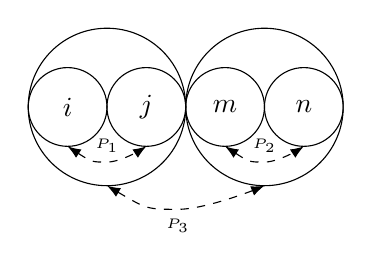
\begin{tikzpicture}[scale=1]
\coordinate (p1) at (2,5) {} {};
\coordinate (p2) at (3,5) {};
\coordinate (p3) at (4,5) {} {} {};
\coordinate (p4) at (5,5) {} {} {};
\coordinate (l1) at (2.5,5) {} {};
\coordinate (l2) at (4.5,5) {};
\draw  (p1) circle(0.5);
\node at (p1)  {$i$};
\draw  (p2) circle(0.5);
\node at (p2)  {$j$};
\draw  (p3) circle(0.5);
\node at (p3)  {$m$};
\draw  (p4) circle(0.5);
\node at (p4)  {$n$};
\draw  (l1) circle(1.);
\draw  (l2) circle(1.);

\draw [Latex-Latex ,dashed] plot[smooth, tension=.7] coordinates {(2,4.5) (2.5,4.3) (3,4.5)};
\draw   [Latex-Latex ,dashed]plot[smooth, tension=.7] coordinates {(4,4.5) (4.5,4.3) (5,4.5)};
\draw   [Latex-Latex ,dashed]plot[smooth, tension=.7] coordinates {(2.5,4) (3.4,3.7) (4.5,4)};
\node[anchor = south ] at (2.5,4.3)   {\tiny$P_1$};
\node[anchor = south ] at (4.5,4.3)  {\tiny$P_2$};
\node[anchor = north ] at (3.4,3.7)  {\tiny$P_3$};
\end{tikzpicture}}
\caption{Permutations}
\label{fig:fig_p247}
\end{figure}
The factor $\frac{1}{8}$ is explained by te fact that are $2^3$ possible permutations in the $i,j,m,n$ indexes i.e. $2\times2$ for the permutations $P_1$ and $P_2$ and again $2$ for the permutation $P_3$. Note that a single permutation $P_1$ or $P_2$ changes the sign of  $T_{ij}T_{mn}$ but also changes the sign of $\delta^{ijmn}_{1234}$, so the combined sign doesn't change. A double permutation $P_1$ and  $P_2$ changes the sign of  $T_{ij}$ and $T_{mn}$ resulting in a unchanged sign of  $T_{ij}T_{mn}$ but also $\delta^{ijmn}_{1234}$ is unchanged because of the double permutation. Finally $P_3$ has no effect, nor on $T_{ij}T_{mn}$ nor on $\delta^{ijmn}_{1234}$. So we have 8 repetitions for  the same set $i,j,m,n$.\\
So we have, 
\begin{align}
P&= \frac{1}{8}\delta^{ijmn}_{1234}T_{ij}T_{mn}\\
&= \frac{1}{8}\epsilon^{ijmn}T_{ij}T_{mn}
\end{align}
From this follows immediately as $\epsilon^{ijmn}$ is a relative tensor of weight $1$ and $T_{ij}$ an absolute tensor (i.e. a relative tensor of weight $0$) that $P$ is a relative tensor of eight $1$ i.e. a density.
$$\blacklozenge$$
\newpage



\section{p247 - Exercise }
\begin{tcolorbox}
Show that, for rectangular Cartesian coordinates, the vorticity tensor and the vorticity vector of a fluid are duals (cf. $\mathbf{6.130}$).
\end{tcolorbox}
$\mathbf{6.130}$:
\begin{align}
\omega_r=\half\epsilon_{rmn}\omega_{mn},\spatie \omega_{mn}=\epsilon_{rmn}\omega_r
\end{align}
Put $\hat{T}^r= \omega_r$ and $T_{mn} = \omega_{mn}$
then the expressions in $(1)$ can be expressed as (considering that the covariant an contravariant expressions are identical in rectangular Cartesian coordinates) 
\begin{align}
\hat{T}^r=\frac{1}{(3-2)!}\epsilon^{mnr}T_{mn},\spatie T_{mn}=\epsilon_{rmn}\hat{T}^r
\end{align}
which are exactly the general definitions $\mathbf{7.121}$ and $\mathbf{7.122}$ (with $N=3$ and $M=2$) for dual tensors.
$$\blacklozenge$$
\newpage


\section{p250 - Exercise }
\begin{tcolorbox}
Show that
$$\eta_{r_1\dots r_N}= \epsilon(a)a_{r_1s_1}\dots a_{r_Ns_N}\eta^{s_1\dots s_N}$$
$$\eta^{r_1\dots r_N}= \epsilon(a)a^{r_1s_1}\dots a^{r_Ns_N}\eta_{s_1\dots s_N}$$
\end{tcolorbox}
$$\blacklozenge$$
\newpage

\section{p252 - Exercise }
\begin{tcolorbox}
Using Riemannian coordinates, prove that 
$\mathbf{7.216}\quad \epsilon_{r_1\dots r_N|k}=\epsilon^{r_1\dots r_N}_{\quad\quad |k}=0$
$\quad \quad \eta_{r_1\dots r_N|k}= \eta^{r_1\dots r_N}_{\quad\quad|k}=0$
\end{tcolorbox}
$$\blacklozenge$$
\newpage




\section{p252 - Exercise }
\begin{tcolorbox}
Prove that if $T^n$ is a relative vector of weight $W$ then,
$$\mathbf{7.220} \quad T^n_{\ |n}= \left(\epsilon(a)a\right)^{\half(W-1)}\pdv{}{x^n}\left[\left(\epsilon(a)a\right)^{\half(1-W)}T^n\right]$$ 
\end{tcolorbox}
$$\blacklozenge$$
\newpage
<<<<<<< HEAD

\section{p255 - Clarification}
\begin{tcolorbox}
$$\mathbf{7.304} \quad \Delta^{k_1\dots k_M}=\delta^{k_1\dots k_M}_{s_1\dots s_M}\Delta_{(1)}x^{s_1} \dots \Delta_{(M)}x^{s_M}$$ 
\end{tcolorbox}
Using $\mathbf{7.303}$ and noting that a permutation of columns in the matrix changes or not  the sign of its determinant depending on the sign of the permutation, we can write 
\begin{align}\Delta^{k_1\dots k_M} &= \left|\begin{matrix}
\Delta_{(1)}x^{k_1}&\Delta_{(1)}x^{k_2} &\dots&\Delta_{(1)}x^{k_M}\\
\Delta_{(2)}x^{k_1}&\Delta_{(2)}x^{k_2} &\dots&\Delta_{(2)}x^{k_M}\\
\vdots&\vdots&\vdots&\vdots\\
\Delta_{(M)}x^{k_1}&\Delta_{(M)}x^{k_2} &\dots&\Delta_{(M)}x^{k_M}\\
\end{matrix}\right|\\
&= \epsilon^{k_1 k_2\dots k_m}\left|\begin{matrix}
\Delta_{(1)}x^{1}&\Delta_{(1)}x^{2} &\dots&\Delta_{(1)}x^{M}\\
\Delta_{(2)}x^{1}&\Delta_{(2)}x^{k_2} &\dots&\Delta_{(2)}x^{k_M}\\
\vdots&\vdots&\vdots&\vdots\\
\Delta_{(M)}x^{1}&\Delta_{(M)}x^{2} &\dots&\Delta_{(M)}x^{M}\\
\end{matrix}\right|
\end{align}
And using $\mathbf{4.313}:\quad \left|A_{pq}\right|= \epsilon_{s_1 s_2 \dots s_M}A_{1 s_1}A_{2 s_2}\dots A_{M s_M}$:
\begin{align}\Delta^{k_1 \dots k_M} &= \underbrace{\epsilon^{k_1 k_2\dots k_m} \epsilon_{s_1 s_2 \dots s_M}}_{\text{see (7.114)}}\Delta_{(1)}x^{s_1}\Delta_{(2)}x^{s_2} \dots \Delta_{(M)}x^{s_M}\\
&= \delta^{k_1\dots k_M}_{s_1\dots s_M}\Delta_{(1)}x^{s_1}\Delta_{(2)}x^{s_2} \dots \Delta_{(M)}x^{s_M}
\end{align}
$$\blacklozenge$$
\newpage

=======

\section{p255 - Clarification}
\begin{tcolorbox}
$$\mathbf{7.304} \quad \Delta^{k_1\dots k_M}=\delta^{k_1\dots k_M}_{s_1\dots s_M}\Delta_{(1)}x^{s_1} \dots \Delta_{(M)}x^{s_M}$$ 
\end{tcolorbox}
Using $\mathbf{7.303}$ and noting that a permutation of columns in the matrix changes or not  the sign of its determinant depending on the sign of the permutation, we can write 
\begin{align}\Delta^{k_1\dots k_M} &= \left|\begin{matrix}
\Delta_{(1)}x^{k_1}&\Delta_{(1)}x^{k_2} &\dots&\Delta_{(1)}x^{k_M}\\
\Delta_{(2)}x^{k_1}&\Delta_{(2)}x^{k_2} &\dots&\Delta_{(2)}x^{k_M}\\
\vdots&\vdots&\vdots&\vdots\\
\Delta_{(M)}x^{k_1}&\Delta_{(M)}x^{k_2} &\dots&\Delta_{(M)}x^{k_M}\\
\end{matrix}\right|\\
&= \epsilon^{k_1 k_2\dots k_m}\left|\begin{matrix}
\Delta_{(1)}x^{1}&\Delta_{(1)}x^{2} &\dots&\Delta_{(1)}x^{M}\\
\Delta_{(2)}x^{1}&\Delta_{(2)}x^{k_2} &\dots&\Delta_{(2)}x^{k_M}\\
\vdots&\vdots&\vdots&\vdots\\
\Delta_{(M)}x^{1}&\Delta_{(M)}x^{2} &\dots&\Delta_{(M)}x^{M}\\
\end{matrix}\right|
\end{align}
And using $\mathbf{4.313}:\quad \left|A_{pq}\right|= \epsilon_{s_1 s_2 \dots s_M}A_{1 s_1}A_{2 s_2}\dots A_{M s_M}$:
\begin{align}\Delta^{k_1 \dots k_M} &= \underbrace{\epsilon^{k_1 k_2\dots k_m} \epsilon_{s_1 s_2 \dots s_M}}_{\text{see (7.114)}}\Delta_{(1)}x^{s_1}\Delta_{(2)}x^{s_2} \dots \Delta_{(M)}x^{s_M}\\
&= \delta^{k_1\dots k_M}_{s_1\dots s_M}\Delta_{(1)}x^{s_1}\Delta_{(2)}x^{s_2} \dots \Delta_{(M)}x^{s_M}
\end{align}
$$\blacklozenge$$
\newpage

>>>>>>> adfdd13a74863c750c19cd7f30af5a98907dce92
\section{p255 - Exercise }
\begin{tcolorbox}
Show that $\mathbf{7.305}$ may be written in the equivalent form
$$d\tau_{(M)}^{k_1\dots k_m}= \epsilon^{\beta_1\dots \beta_M}d_{(\beta_1)}x^{k_1}\dots d_{(\beta_M)}x^{k_M}$$
\end{tcolorbox}
The determinant of a matrix and its transpose are equal.\\
Hence we can rewrite $\mathbf{7.305} \quad \delta^{k_1\dots k_M}_{s_1\dots s_M}d_{(1)}x^{s_1}\dots d_{(M)}x^{s_M}$ as
\begin{align}
d\tau_{(M)}^{k_1\dots k_m}=\delta_{k_1\dots k_M}^{s_1\dots s_M}d_{(s_1)}x^{1}\dots d_{(s_M)}x^{M}
\end{align}
In order to be consistent with the notation we replace the $s_i$ by $\alpha_i$ as the summation occurs along the constants $c^{(i)}$
\begin{align}
d\tau_{(M)}^{k_1\dots k_m}=\delta_{k_1\dots k_M}^{\alpha_1\dots \alpha_M}d_{(\alpha_1)}x^{1}\dots d_{(\alpha_M)}x^{M}
\end{align}
Given the set $\{k_1, k_2,\dots , k_M\}$ we can represent the sequence $\{1,2,\dots , M\}$ by $\{k_j, k_m,\dots ,k_M,\dots k_n\}$ (imagine that $k_j=1, k_m=2,...$ etc.). We rewrite $(2)$ as
\begin{align}
d\tau_{(M)}^{k_1 k_2\dots k_m}=(\theta_{\alpha}) \delta_{1 2 \dots M}^{\alpha_1\dots \alpha_M}d_{(\alpha_1)}x^{k_j}d_{(\alpha_2)}x^{k_m}\dots d_{(\alpha_M)}x^{k_n}
\end{align}
where 
\begin{align}
\theta_{\alpha} = \epsilon_{k_1 k_2\dots k_M}
\end{align}
( a permutation in the lower indexes of the generalized Kronecker deltas symbol will invert the sign depending on the 'oddness' of the permutation).
Let's rearrange the product $d_{(\alpha_1)}x^{k_j}d_{(\alpha_2)}x^{k_m}\dots d_{(\alpha_M)}x^{k_n}$ so that the indexes $k_i$ are naturally ordered
\begin{align}
d\tau_{(M)}^{k_1 k_2\dots k_m}=(\theta_{\alpha}) \delta_{1 2 \dots M}^{\alpha_1\dots \alpha_M}d_{(\alpha_r)}x^{k_1}d_{(\alpha_n)}x^{k_2}\dots d_{(\alpha_1)}x^{k_n}\dots d_{(\alpha_s)}x^{k_M}
\end{align}
and changing the order in the upper indexes of the general Kroneckers delta's:
\begin{align}
d\tau_{(M)}^{k_1 k_2\dots k_m}=(\theta_{\alpha})(\theta_{k}) \delta_{1 2 \dots M}^{\alpha_r\alpha_n \dots \alpha_s}d_{(\alpha_r)}x^{k_1}d_{(\alpha_n)}x^{k_2}\dots d_{(\alpha_1)}x^{k_n}\dots d_{(\alpha_s)}x^{k_M}
\end{align}
where $\theta_{k}= \pm 1$ depending on the 'oddness' of the permutation needed to go from $\{\alpha_1\dots \alpha_M\}$ to $\{\alpha_r\alpha_n \dots \alpha_s\}$.\\
As we can see in figure $7.2$,  it's no hard to see that 
\begin{align}
\theta_{k}=\theta_{\alpha}
\end{align}
\begin{figure}[H]%
    \centering
    \subfloat[]{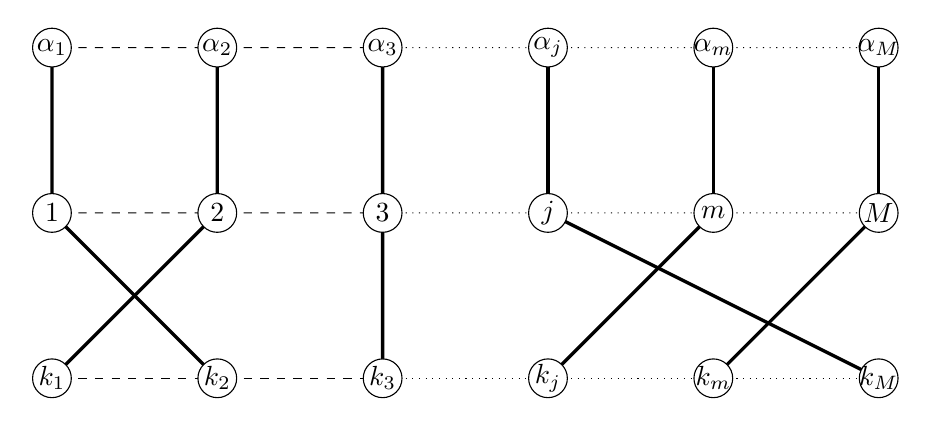
\begin{tikzpicture}[scale=0.7]


\node (alfa1) at (-10,6) {};
\node (alfaM) at (5,6) {};
\node (alfa2)at (-7,6) {};
\node (alfa3) at (-4,6) {};
\node (alfa4)at (-1,6) {};
\node (alfa5)at (2,6) {};

\node (v1) at (-10,3) {};
\node (vM) at (5,3) {};
\node (v2)at (-7,3) {};
\node (v3) at (-4,3) {};
\node (v4)at (-1,3) {};
\node (v5)at (2,3) {};

\node (k1) at (-10,0) {};
\node (kM) at (5,0) {};
\node (k2)at (-7,0) {};
\node (k3) at (-4,0) {};
\node (k4)at (-1,0) {};
\node (k5)at (2,0) {};


\draw[very thick]  (alfa1) --(v1);
\draw[very thick]  (alfa2) --(v2);
\draw[very thick]  (alfa3) --(v3);
\draw[very thick]  (alfa4) --(v4);
\draw[very thick]  (alfa5) --(v5);
\draw[very thick]  (alfaM) --(vM);
\draw[very thick]  (k2) --(v1);
\draw[very thick]  (k1) --(v2);
\draw[very thick]  (k3) --(v3);
\draw[very thick]  (kM) --(v4);
\draw[very thick]  (k4) --(v5);
\draw[very thick]  (k5) --(vM);



\draw[dashed]  (alfa1) --(alfa2);
\draw[dashed]  (alfa2) --(alfa3);
\draw[dotted]  (alfa3) --(alfa4);
\draw[dotted]  (alfa4) --(alfa5);
\draw [dotted](alfa5) --(alfaM);

\draw  [fill= white](alfa1)circle (10pt);
\draw  [fill= white](alfaM)circle (10pt);
\draw  [fill= white](alfa2)circle (10pt);
\draw  [fill= white](alfa3)circle (10pt);
\draw  [fill= white](alfa4)circle (10pt);
\draw  [fill= white](alfa5)circle (10pt);

\node[] at (alfa1)  {$\alpha_1$};
\node[] at (alfaM)  {$\alpha_M$};
\node[] at (alfa2)  {$\alpha_2$};
\node[] at (alfa3)  {$\alpha_3$};
\node[] at (alfa4)  {$\alpha_j$};
\node[] at (alfa5)  {$\alpha_m$};



\draw [dashed] (v1) --(v2);
\draw[dashed]  (v2) --(v3);
\draw[dotted]  (v3) --(v4);
\draw[dotted]  (v4) --(v5);

\draw  [dotted](v5) --(vM);
\draw  [fill= white](v1)circle (10pt);
\draw  [fill= white](vM)circle (10pt);
\draw  [fill= white](v2)circle (10pt);
\draw  [fill= white](v3)circle (10pt);
\draw  [fill= white](v4)circle (10pt);
\draw  [fill= white](v5)circle (10pt);

\node[] at (v1)  {$1$};
\node[] at (vM)  {$M$};
\node[] at (v2)  {$2$};
\node[] at (v3)  {$3$};
\node[] at (v4)  {$j$};
\node[] at (v5)  {$m$};



\draw[dashed]  (k1) --(k2);
\draw[dashed]  (k2) --(k3);
\draw[dotted]  (k3) --(k4);
\draw[dotted]  (k4) --(k5);

\draw  [dotted](k5) --(kM);
\draw  [fill= white](k1)circle (10pt);
\draw  [fill= white](kM)circle (10pt);
\draw  [fill= white](k2)circle (10pt);
\draw  [fill= white](k3)circle (10pt);
\draw  [fill= white](k4)circle (10pt);
\draw  [fill= white](k5)circle (10pt);

\node[] at (k1)  {$k_1$};
\node[] at (kM)  {$k_M$};
\node[] at (k2)  {$k_2$};
\node[] at (k3)  {$k_3$};
\node[] at (k4)  {$k_j$};
\node[] at (k5)  {$k_m$};


\end{tikzpicture}}\\
    \subfloat[]{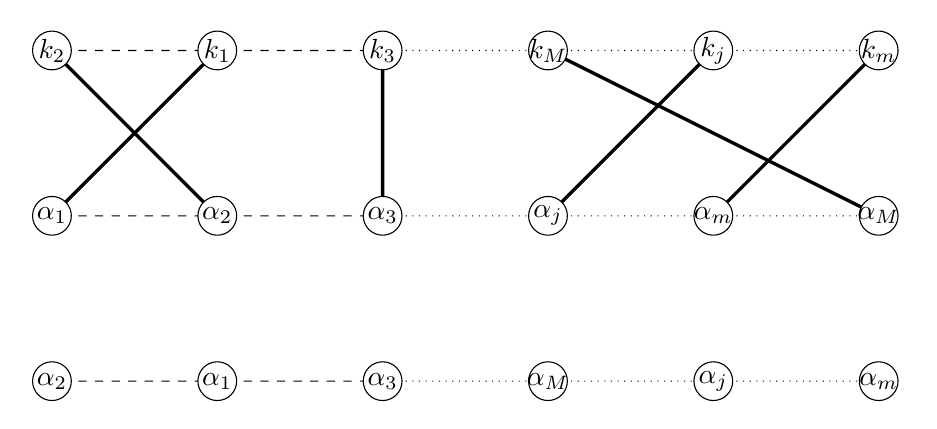
\begin{tikzpicture}[scale=0.7]


\node (alfaPR1) at (-10,-9) {};
\node (alfaPRM) at (5,-9) {};
\node (alfaPR2)at (-7,-9) {};
\node (alfaPR3) at (-4,-9) {};
\node (alfaPR4)at (-1,-9) {};
\node (alfaPR5)at (2,-9) {};

\node (alfaP1) at (-10,-6) {};
\node (alfaPM) at (5,-6) {};
\node (alfaP2)at (-7,-6) {};
\node (alfaP3) at (-4,-6) {};
\node (alfaP4)at (-1,-6) {};
\node (alfaP5)at (2,-6) {};

\node (kp1) at (-10,-3) {};
\node (kpM) at (5,-3) {};
\node (kp2)at (-7,-3) {};
\node (kp3) at (-4,-3) {};
\node (kp4)at (-1,-3) {};
\node (kp5)at (2,-3) {};



\draw[very thick]  (alfaP2) --(kp1);
\draw[very thick]  (alfaP1) --(kp2);
\draw[very thick]  (alfaP3) --(kp3);
\draw[very thick]  (alfaPM) --(kp4);
\draw[very thick]  (alfaP4) --(kp5);
\draw[very thick]  (alfaP5) --(kpM);



\draw [dashed] (kp1) --(kp2);
\draw [dashed] (kp2) --(kp3);
\draw[dotted]  (kp3) --(kp4);
\draw[dotted]  (kp4) --(kp5);
\draw  [dotted](kp5) --(kpM);

\draw  [fill= white](kp1)circle (10pt);
\draw  [fill= white](kpM)circle (10pt);
\draw  [fill= white](kp2)circle (10pt);
\draw  [fill= white](kp3)circle (10pt);
\draw  [fill= white](kp4)circle (10pt);
\draw  [fill= white](kp5)circle (10pt);

\node[] at (kp1)  {$k_2$};
\node[] at (kpM)  {$k_m$};
\node[] at (kp2)  {$k_1$};
\node[] at (kp3)  {$k_3$};
\node[] at (kp4)  {$k_M$};
\node[] at (kp5)  {$k_j$};

\draw[dashed]  (alfaP1) --(alfaP2);
\draw[dashed]  (alfaP2) --(alfaP3);
\draw[dotted]  (alfaP3) --(alfaP4);
\draw[dotted]  (alfaP4) --(alfaP5);
\draw [dotted](alfaP5) --(alfaPM);

\draw[dashed]  (alfaPR1) --(alfaPR2);
\draw[dashed]  (alfaPR2) --(alfaPR3);
\draw[dotted]  (alfaPR3) --(alfaPR4);
\draw[dotted]  (alfaPR4) --(alfaPR5);
\draw [dotted](alfaPR5) --(alfaPRM);

\draw  [fill= white](alfaP1)circle (10pt);
\draw  [fill= white](alfaPM)circle (10pt);
\draw  [fill= white](alfaP2)circle (10pt);
\draw  [fill= white](alfaP3)circle (10pt);
\draw  [fill= white](alfaP4)circle (10pt);
\draw  [fill= white](alfaP5)circle (10pt);

\draw  [fill= white](alfaPR1)circle (10pt);
\draw  [fill= white](alfaPRM)circle (10pt);
\draw  [fill= white](alfaPR2)circle (10pt);
\draw  [fill= white](alfaPR3)circle (10pt);
\draw  [fill= white](alfaPR4)circle (10pt);
\draw  [fill= white](alfaPR5)circle (10pt);

\node[] at (alfaP1)  {$\alpha_1$};
\node[] at (alfaPM)  {$\alpha_M$};
\node[] at (alfaP2)  {$\alpha_2$};
\node[] at (alfaP3)  {$\alpha_3$};
\node[] at (alfaP4)  {$\alpha_j$};
\node[] at (alfaP5)  {$\alpha_m$};

\node[] at (alfaPR1)  {$\alpha_2$};
\node[] at (alfaPRM)  {$\alpha_m$};
\node[] at (alfaPR2)  {$\alpha_1$};
\node[] at (alfaPR3)  {$\alpha_3$};
\node[] at (alfaPR4)  {$\alpha_M$};
\node[] at (alfaPR5)  {$\alpha_j$};
\end{tikzpicture}}
\caption{Permutations}
\label{fig:fig_p255}
\end{figure}
Indeed suppose, as in the example $(a)$ ,  $k_1=2, k_2=1,k_3=3, ,\dots ,k_j = m,\dots , k_m=j,\dots$ etc., so we get a sequence $\{k_2, k_1,k_3,\dots, k_m,\dots k_j,\dots\}$ as illustrated in $(b)$. But to have - with this sequence - an equivalent expression of 
$d\tau_{(M)}^{k_1 k_2\dots k_m}=(\theta_{\alpha}) \delta_{1 2 \dots M}^{\alpha_1\dots \alpha_M}d_{(\alpha_1)}x^{k_j}d_{(\alpha_2)}x^{k_m}\dots d_{(\alpha_M)}x^{k_n}$, we need to make an equivalent permutation so that $\alpha_r$ gets in the same position  as $k_r$, resulting in a new sequence $\{\alpha_2,\alpha_1,\alpha_3,\dots,\alpha_M,\dots,\alpha_j, \alpha_m\}$.\\
The number of permutations to generate $\theta_{\alpha}$ and $\theta_k$ are identical resulting in $\theta_{\alpha}\theta_k=1$.
So $(6)$ can be rewritten (noting that the $\alpha_r$ are dummy indexes and that we are free to rename them so that $r=1, n=2,\dots$) 
\begin{align}
d\tau_{(M)}^{k_1 k_2\dots k_m}= \delta_{1 2 \dots M}^{\beta_1\beta_2 \dots \beta_M}d_{(\beta_1)}x^{k_1}d_{(\beta_2)}x^{k_2}\dots d_{(\beta_n)}x^{k_n}\dots d_{(\beta_M)}x^{k_M}
\end{align}
Finally, using $\mathbf{7.114}$ 
\begin{align}
d\tau_{(M)}^{k_1 k_2\dots k_m}&= \underbrace{\epsilon_{1 2 \dots M}}_{=1}\epsilon^{\beta_1\beta_2 \dots \beta_M}d_{(\beta_1)}x^{k_1}d_{(\beta_2)}x^{k_2}\dots d_{(\beta_n)}x^{k_n}\dots d_{(\beta_M)}x^{k_M}\\
&= \epsilon^{\beta_1\beta_2 \dots \beta_M}d_{(\beta_1)}x^{k_1}d_{(\beta_2)}x^{k_2}\dots d_{(\beta_n)}x^{k_n}\dots d_{(\beta_M)}x^{k_M}
\end{align}
$$\blacklozenge$$
\newpage


\section{p257 - Exercise }
\begin{tcolorbox}
Let $x^k$ be rectangular Cartesian coordinates in Euclidean $3-$space. Introduce polar coordinates $r,\theta,\phi$ and consider the surface of the sphere $r=a$. On this sphere form the infinitesimal $2-$cell with corners $(\theta,\phi),\ (\theta+d\theta,\phi),\ (\theta,\phi+d\phi),\ (\theta+d\theta,\phi+d\phi)$. Determine the extension of this cell and interpret the rectangular components. In particular, show that the three independent components of the extension are (apart from the sign) equal to the areas obtained by normal projection of the cell onto the three rectangular planes. Does this interpretation remain valid if the sphere is replaces by some other surface?
\end{tcolorbox}
We use $\mathbf{7.312}$:
\begin{align}
d\tau_{(2)}^{k_1k_2}&= \epsilon^{\alpha_1\alpha_2}\pdv{x^{k_1}}{y^{\alpha_1}}\pdv{x^{k_2}}{y^{\alpha_2}}\left|d_{(\beta)}y^{\gamma}\right|
\end{align}
with $(y^1, y^2)= (\theta,\phi)$ giving if we take $f^{(i)}=c^{(i)} $ as $\theta=c^{(1)},\ \phi =c^{(2)} $:
\begin{align}
\left|d_{(\beta)}y^{\gamma}\right|&=\left|\begin{matrix}d_{(1)}y^{1}&d_{(1)}y^{2}\\
d_{(2)}y^{1}&d_{(2)}y^{2}\end{matrix}\right|\\
&=\left|\begin{matrix}d{\theta}&0\\
0&d{\phi}\end{matrix}\right|\\
&= d{\theta}d{\phi}
\end{align}
We also have
\begin{align}
\left\{\begin{array}{l}
x= a\sin{\theta}\cos{\phi}\\
y= a\sin{\theta}\sin{\phi}\\
z= a\cos{\theta}\\
\end{array}\right.\\
\end{align}
giving
\begin{align}
\left\{\begin{array}{l}
\pdv{x}{\theta}= a\cos{\theta}\cos{\phi}\\
\pdv{x}{\phi}= -a\sin{\theta}\sin{\phi}\\
\pdv{y}{\theta}= a\cos{\theta}\sin{\phi}\\
\pdv{y}{\phi}=  a\sin{\theta}\cos{\phi}\\
\pdv{z}{\theta}= -a\sin{\theta}\\
\pdv{z}{\phi}= 0\\
\end{array}\right.\\
\end{align}

and get 
\begin{align}
d\tau_{(2)}^{xy}&= \underbrace{\epsilon^{11}}_{=0}\pdv{x}{\theta}\pdv{y}{\theta}d{\theta}d{\phi}+\epsilon^{12}\pdv{x}{\theta}\pdv{y}{\phi}d{\theta}d{\phi}+\epsilon^{21}\pdv{x}{\phi}\pdv{y}{\theta}d{\theta}d{\phi}+\underbrace{\epsilon^{22}}_{=0}\pdv{x}{\phi}\pdv{y}{\phi}d{\theta}d{\phi}\\
&=a^2\cos{\theta}\cos{\phi}\sin{\theta}\cos{\phi}d{\theta}d{\phi}
+a^2\sin{\theta}\sin{\phi}\cos{\theta}\sin{\phi}d{\theta}d{\phi}\\
&=a^2\cos{\theta}\sin{\theta}d{\theta}d{\phi}\\
d\tau_{(2)}^{yx}&=-a^2\cos{\theta}\sin{\theta}d{\theta}d{\phi}
\end{align}
\begin{align}
d\tau_{(2)}^{xz}&= \underbrace{\epsilon^{11}}_{=0}\pdv{x}{\theta}\pdv{z}{\theta}d{\theta}d{\phi}+\epsilon^{12}\pdv{x}{\theta}\underbrace{\pdv{z}{\phi}}_{=0}d{\theta}d{\phi}+\epsilon^{21}\pdv{x}{\phi}\pdv{z}{\theta}d{\theta}d{\phi}+\underbrace{\epsilon^{22}}_{=0}\pdv{x}{\phi}\pdv{z}{\phi}d{\theta}d{\phi}\\
&=-a^2\sin^2{\theta}\sin{\phi}d{\theta}d{\phi}\\
d\tau_{(2)}^{zx}&=a^2\sin^2{\theta}\sin{\phi}d{\theta}d{\phi}
\end{align}
\begin{align}
d\tau_{(2)}^{yz}&= \underbrace{\epsilon^{11}}_{=0}\pdv{y}{\theta}\pdv{z}{\theta}d{\theta}d{\phi}+\epsilon^{12}\pdv{y}{\theta}\underbrace{\pdv{z}{\phi}}_{=0}d{\theta}d{\phi}+\epsilon^{21}\pdv{y}{\phi}\pdv{z}{\theta}d{\theta}d{\phi}+\underbrace{\epsilon^{22}}_{=0}\pdv{y}{\phi}\pdv{z}{\phi}d{\theta}d{\phi}\\
&=a^2\sin^2{\theta}\cos{\phi}d{\theta}d{\phi}\\
d\tau_{(2)}^{zy}&=-a^2\sin^2{\theta}\cos{\phi}d{\theta}d{\phi}
\end{align}
\begin{align}
d\tau_{(2)}^{xx}&= \underbrace{\epsilon^{11}}_{=0}\pdv{x}{\theta}\pdv{x}{\theta}d{\theta}d{\phi}+\epsilon^{12}\pdv{x}{\theta}\pdv{x}{\phi}d{\theta}d{\phi}+\epsilon^{21}\pdv{x}{\phi}\pdv{x}{\theta}d{\theta}d{\phi}+\underbrace{\epsilon^{22}}_{=0}\pdv{x}{\phi}\pdv{x}{\phi}d{\theta}d{\phi}\\
&=0
\end{align}

\begin{align}
d\tau_{(2)}^{yy}&= \underbrace{\epsilon^{11}}_{=0}\pdv{y}{\theta}\pdv{y}{\theta}d{\theta}d{\phi}+\epsilon^{12}\pdv{y}{\theta}\pdv{y}{\phi}d{\theta}d{\phi}+\epsilon^{21}\pdv{y}{\phi}\pdv{y}{\theta}d{\theta}d{\phi}+\underbrace{\epsilon^{22}}_{=0}\pdv{y}{\phi}\pdv{y}{\phi}d{\theta}d{\phi}\\
&=0
\end{align}

\begin{align}
d\tau_{(2)}^{zz}&= \underbrace{\epsilon^{11}}_{=0}\pdv{z}{\theta}\pdv{z}{\theta}d{\theta}d{\phi}+\epsilon^{12}\pdv{z}{\theta}\underbrace{\pdv{z}{\phi}}_{=0}d{\theta}d{\phi}+\epsilon^{21}\underbrace{\pdv{z}{\phi}}_{=0}\pdv{z}{\theta}d{\theta}d{\phi}+\underbrace{\epsilon^{22}}_{=0}\pdv{z}{\phi}\pdv{z}{\phi}d{\theta}d{\phi}\\
&=0
\end{align}
\begin{figure}[H]%
    \centering
    \subfloat[]{
%Axis Angles  
\tdplotsetmaincoords{70}{110}

%Macros  
\pgfmathsetmacro{\rvec}{7.5}  
\pgfmathsetmacro{\thetavec}{40}  
\pgfmathsetmacro{\phivec}{45}

\pgfmathsetmacro{\dphivec}{20}  
\pgfmathsetmacro{\dthetavec}{20}  

%Layers  
\pgfdeclarelayer{background} 
\pgfdeclarelayer{foreground}

\pgfsetlayers{background, main, foreground}
\begin{tikzpicture}
	[scale=0.8,
		tdplot_main_coords,
		axis/.style={->,black,thick},
		vector/.style={-stealth,black, thick},
		vector guide/.style={dashed,black,thick},
		angle/.style={black,thick}]

	%standard tikz coordinate definition using x, y, z coords
	\coordinate (O) at (0,0,0);

\tdplotsetcoord{E}{\rvec }{\thetavec}{\phivec}  
\tdplotsetcoord{F}{\rvec }{\thetavec + \dthetavec}{\phivec}  
\tdplotsetcoord{F'}{\rvec }{90}{\phivec}  \tdplotsetcoord{G}{\rvec }{\thetavec + \dthetavec}{\phivec + \dphivec}  
\tdplotsetcoord{G'}{\rvec }{90}{\phivec + \dphivec} 
\tdplotsetcoord{H}{\rvec }{\thetavec}{\phivec + \dphivec} 
    
%Axis  
\begin{pgfonlayer}{background}  
    \draw[thick,-latex] (0,0,0) -- (7,0,0) node[pos=1.1]{$x$};        
    \draw[thick,-latex] (0,0,0) -- (0,7,0) node[pos=1.05]{$y$};         
    \draw[thick,-latex] (0,0,0) -- (0,0,6) node[pos=1.05]{$z$};                   
\end{pgfonlayer}

%Help Lines  
\begin{pgfonlayer}{background}  
    %Up     
      
   
  
    %Down   
    \draw[dashed] (O) -- (F');  
    \draw[dashed] (O) -- (G');  
\end{pgfonlayer}  
\begin{pgfonlayer}{foreground}  
    %%Help Curves   
    \tdplotsetthetaplanecoords{\phivec}     
    %
    \tdplotdrawarc[dotted,tdplot_rotated_coords]{(O)}{\rvec}{\thetavec+\dthetavec}{90}{}{}
    %
    \tdplotsetthetaplanecoords{\phivec+\dphivec}    
    \tdplotdrawarc[dotted,tdplot_rotated_coords]{(O)}{\rvec}{\thetavec+\dthetavec}{90}{}{}

    %    
    \tdplotdrawarc[dotted,tdplot_main_coords]{(O)}{\rvec}{\phivec}{\phivec+\dphivec}{below, rotate=13}{} 
\end{pgfonlayer}


%Angles  
\begin{pgfonlayer}{foreground}  
    %Phi, dPhi  
    \tdplotdrawarc[-stealth]{(O)}{0.9}{0}{\phivec}{anchor=north}{$\phi$}    
    \tdplotdrawarc[-stealth]{(O)}{1.5}{\phivec}{\phivec + \dphivec}{}{} 
    \node at (1.4,1.9,0) {$\mathrm{d}\phi$};        
    \tdplotsetthetaplanecoords{\phivec}     
    %Theta, dTheta          
    \tdplotdrawarc[tdplot_rotated_coords,-stealth]{(0,0,0)}{1.2}{0}{\thetavec}{}{}      
    \node at (0,0.3,1.3) {$\theta$};    
    \tdplotdrawarc[tdplot_rotated_coords,-stealth]{(0,0,0)}{2.5}{\thetavec}{\thetavec + \dthetavec}{anchor=south west}{$\mathrm{d}\theta$}  
\end{pgfonlayer}

%Differential Volume

%%Lines  
\begin{pgfonlayer}{foreground}  
    \draw[dashed] (O) -- (E) node[midway, above left]{a};    
    \draw[dashed] (O) -- (F);    
    \draw[dashed] (O) -- (G);      
\end{pgfonlayer}   
\begin{pgfonlayer}{background}
    \draw[dashed] (O) -- (H);  
\end{pgfonlayer}

%%Curved 

 \begin{pgfonlayer}{foreground}     
    \tdplotsetthetaplanecoords{\phivec}       
    \tdplotdrawarc[tdplot_rotated_coords, thick]{(O)}{\rvec }{\thetavec}{\dthetavec + \thetavec}{}{}
    %   
    \tdplotsetthetaplanecoords{\phivec + \dphivec}  
    \tdplotdrawarc[tdplot_rotated_coords, thick]{(O)}{\rvec }{\thetavec}{\dthetavec + \thetavec}{above right}{$a\mathrm{d}\theta$}  
    %   
    \tdplotsetrotatedcoords{55}{-50.4313}{-6.4086}  
    \tdplotdrawarc[tdplot_rotated_coords, thick]{(O)}{\rvec }{0}{12.8173}{anchor=south }{$a\sin\theta\mathrm{d}\phi$}      
    %   
    \tdplotsetrotatedcoords{55}{-30.3813}{-8.6492}          
    \tdplotdrawarc[tdplot_rotated_coords, thick]{(O)}{\rvec}{0}{17.2983}{}{}  
\end{pgfonlayer}

%Fill Color 
\begin{pgfonlayer}{main}    
    %Front  
    \fill[gray, opacity=0.2] (E) to[bend left=4] (F)  to[bend left=2] (G) to[bend right=6.5] (H) to[bend right=4] cycle;   
\end{pgfonlayer}  

%\node at (E) {E};
%\node at (F) {F};
%\node at (G) {G};
%\node at (H) {H};
\end{tikzpicture}
}\\
    \subfloat[]{
%Axis Angles  
\tdplotsetmaincoords{75}{120}
%\tdplotsetmaincoords{90}{0}

%Macros  
\pgfmathsetmacro{\rvec}{7.5}  
\pgfmathsetmacro{\thetavec}{60}  
\pgfmathsetmacro{\phivec}{60}

\pgfmathsetmacro{\dphivec}{20}  
\pgfmathsetmacro{\dthetavec}{10}  

%Layers  
\pgfdeclarelayer{background} 
\pgfdeclarelayer{foreground}

\pgfsetlayers{background, main, foreground}
\begin{tikzpicture}
	[scale=1,
		tdplot_main_coords,
		axis/.style={->,black,thick},
		vector/.style={-stealth,black, thick},
		vector guide/.style={dashed,black,thick},
		angle/.style={black,thick}]

	%standard tikz coordinate definition using x, y, z coords
	\coordinate (O) at (0,0,0);

\tdplotsetcoord{E}{\rvec }{\thetavec}{\phivec}  
\tdplotsetcoord{F}{\rvec }{\thetavec + \dthetavec}{\phivec}  
\tdplotsetcoord{F'}{\rvec/3 }{90}{\phivec}  
\tdplotsetcoord{G}{\rvec }{\thetavec + \dthetavec}{\phivec + \dphivec}  
\tdplotsetcoord{G'}{\rvec /3}{90}{\phivec + \dphivec} 
\tdplotsetcoord{H}{\rvec }{\thetavec}{\phivec + \dphivec} 

%\coordinate (E") at {0,\rvec*sin(\phivec )*cos(\thetavec ),100*\rvec*cos(\phivec )};
\draw[dotted] (E) -- (Exz); 
\draw[dotted] (H) -- (Hxz) ;
\draw[dotted] (F) -- (Fxz) ;
\draw[dotted] (G) -- (Gxz) ;
\draw[thick] (Exz) -- (Hxz)-- (Gxz)-- (Fxz) -- cycle;
\draw[thick] (E) -- (H)-- (G)-- (F) -- cycle;


\draw [fill=white](E)circle (1.5pt);
    
%Axis  
\begin{pgfonlayer}{background}  
    \draw[thick,-latex] (0,0,0) -- (5,0,0) node[pos=1.1]{$x$};        
    \draw[thick,-latex] (0,0,0) -- (0,6,0) node[pos=1.05]{$y$};         
    \draw[thick,-latex] (0,0,0) -- (0,0,4.5) node[pos=1.05]{$z$};                   
\end{pgfonlayer}

%Help Lines  
\begin{pgfonlayer}{background}  
    %Up     
      
   
  
    %Down   
    \draw[dashed,ultra thin](O) -- (F');  
    \draw[dashed,ultra thin] (O) -- (G');  
\end{pgfonlayer}  

%Angles  
\begin{pgfonlayer}{foreground}  
    %Phi, dPhi  
    \tdplotdrawarc[-stealth]{(O)}{0.9}{0}{\phivec}{anchor=north}{$\phi$}    
    \tdplotdrawarc[-stealth]{(O)}{1.5}{\phivec}{\phivec + \dphivec}{}{} 
    \node at (1.4,1.9,0) {$\mathrm{d}\phi$};        
    \tdplotsetthetaplanecoords{\phivec}     
    %Theta, dTheta          
    \tdplotdrawarc[tdplot_rotated_coords,-stealth]{(0,0,0)}{1.2}{0}{\thetavec}{}{}      
    \node at (0,0.3,1.3) {$\theta$};    
    \tdplotdrawarc[tdplot_rotated_coords,-stealth]{(0,0,0)}{2.5}{\thetavec}{\thetavec + \dthetavec}{anchor=south west}{$\mathrm{d}\theta$}  
\end{pgfonlayer}

%Differential Volume

%%Lines  
\begin{pgfonlayer}{foreground}  
    \draw[dashed,ultra thin] (O) -- (E) ;%node[midway, above left]{a};    
    \draw[dashed,ultra thin](O) -- (F);    
    \draw[dashed,ultra thin](O) -- (G);      
\end{pgfonlayer}   
\begin{pgfonlayer}{background}
   \draw[dashed,ultra thin] (O) -- (H);  
\end{pgfonlayer}

%%Curved 



%Fill Color 
\begin{pgfonlayer}{main}    
    %Front  
    \fill[gray, opacity=0.2] (E) to[bend left=4] (F)  to[bend left=2] (G) to[bend right=6.5] (H) to[bend right=4] cycle;  
\fill[gray, opacity=0.2] (Exz) to[bend left=4] (Fxz)  to[bend left=2] (Gxz) to[bend right=6.5] (Hxz) to[bend right=4] cycle;      
\end{pgfonlayer}  


\node[anchor=north west] at (H) {$\quad ad\theta$};
\node[anchor=north west] at (F) {$\quad a\sin{\theta}d\phi$};
\node[anchor=south east] at (Gxz) {$ a\sin{\theta}d\theta \quad\quad \quad$};
\node[anchor=south ] at (Exz) {$a\sin{\theta}\sin{\phi}d\phi \quad\quad \quad \quad$};
\begin{pgfonlayer}{foreground}  
    %\draw[dashdotted, thick] (E) -- (Exy) ;  
    %\draw[dashdotted,thick] (E) -- (Eyz) ;  
\end{pgfonlayer} 

  

\coordinate (P) at (2.5,5.2,-0.12);
\draw [fill=white](P)circle (1.5pt);

\coordinate (P') at (2.8,6.2,-0.18);
\draw [fill=white](P')circle (1.5pt);
\draw[dashdotted,thick] (F) -- (P'); 
\draw[dashdotted,thick] (E) -- (P); 
%Angles  
\begin{pgfonlayer}{foreground}  
    %Phi, dPhi  
\tdplotsetthetaplanecoords{\thetavec} 
    \tdplotdrawarc[tdplot_rotated_coords,-stealth]{(E)}{-3.65}{1}{-24}{}{};          
\node[anchor=north east] at (P'){$\frac{\pi}{2}-\theta$};
\end{pgfonlayer}

\coordinate (Q) at (Eyz);
\draw [fill=white](Q)circle (1.5pt);

\coordinate (Q') at (0,6.7,3.73);
\draw [fill=white](Q')circle (1.5pt);
\draw[dashdotted,thick] (E) -- (Q); 
\draw[dashdotted,thick] (H) -- (Q'); 
%Angles  
\begin{pgfonlayer}{foreground}  
    %Phi, dPhi  
\tdplotsetthetaplanecoords{\thetavec} ;
    \tdplotdrawarc[-stealth]{(E)}{-3.4}{1}{-17}{}{};          
\node[anchor=south west] at (Q){$\quad\quad \frac{\pi}{2}-\phi$};
\end{pgfonlayer}
\end{tikzpicture}
}\\
    \subfloat[]{
\tdplotsetmaincoords{75}{120}
%\tdplotsetmaincoords{90}{0}

%Macros  
\pgfmathsetmacro{\rvec}{7.5}  
\pgfmathsetmacro{\thetavec}{60}  
\pgfmathsetmacro{\phivec}{60}

\pgfmathsetmacro{\dphivec}{20}  
\pgfmathsetmacro{\dthetavec}{10}  

%Layers  
\pgfdeclarelayer{background} 
\pgfdeclarelayer{foreground}

\pgfsetlayers{background, main, foreground}
\begin{tikzpicture}
	[scale=1,
		tdplot_main_coords,
		axis/.style={->,black,thick},
		vector/.style={-stealth,black, thick},
		vector guide/.style={dashed,black,thick},
		angle/.style={black,thick}]

	%standard tikz coordinate definition using x, y, z coords
	\coordinate (O) at (0,0,0);

\tdplotsetcoord{E}{\rvec }{\thetavec}{\phivec}  
\tdplotsetcoord{F}{\rvec }{\thetavec + \dthetavec}{\phivec}  
\tdplotsetcoord{F'}{\rvec/3 }{90}{\phivec}  
\tdplotsetcoord{G}{\rvec }{\thetavec + \dthetavec}{\phivec + \dphivec}  
\tdplotsetcoord{G'}{\rvec /3}{90}{\phivec + \dphivec} 
\tdplotsetcoord{H}{\rvec }{\thetavec}{\phivec + \dphivec} 

%\coordinate (E") at {0,\rvec*sin(\phivec )*cos(\thetavec ),100*\rvec*cos(\phivec )};
\draw[dotted] (E) -- (Exy); 
\draw[dotted] (H) -- (Hxy) ;
\draw[dotted] (F) -- (Fxy) ;
\draw[dotted] (G) -- (Gxy) ;
\draw[thick] (Exy) -- (Hxy)-- (Gxy)-- (Fxy) -- cycle;
\draw[thick] (E) -- (H)-- (G)-- (F) -- cycle;


\draw [fill=white](E)circle (1.5pt);
    
%Axis  
\begin{pgfonlayer}{background}  
    \draw[thick,-latex] (0,0,0) -- (5,0,0) node[pos=1.1]{$x$};        
    \draw[thick,-latex] (0,0,0) -- (0,9,0) node[pos=1.05]{$y$};         
    \draw[thick,-latex] (0,0,0) -- (0,0,4.5) node[pos=1.05]{$z$};                   
\end{pgfonlayer}

%Help Lines  
\begin{pgfonlayer}{background}  
    %Up     
      
   
  
    %Down   
    \draw[dashed,ultra thin](O) -- (F');  
    \draw[dashed,ultra thin] (O) -- (G');  
\end{pgfonlayer}  

%Angles  
\begin{pgfonlayer}{foreground}  
    %Phi, dPhi  
    \tdplotdrawarc[-stealth]{(O)}{0.9}{0}{\phivec}{anchor=north}{$\phi$}    
    \tdplotdrawarc[-stealth]{(O)}{1.5}{\phivec}{\phivec + \dphivec}{}{} 
    \node at (1.4,1.9,0) {$\mathrm{d}\phi$};        
    \tdplotsetthetaplanecoords{\phivec}     
    %Theta, dTheta          
    \tdplotdrawarc[tdplot_rotated_coords,-stealth]{(0,0,0)}{1.2}{0}{\thetavec}{}{}      
    \node at (0,0.3,1.3) {$\theta$};    
    \tdplotdrawarc[tdplot_rotated_coords,-stealth]{(0,0,0)}{2.5}{\thetavec}{\thetavec + \dthetavec}{anchor=south west}{$\mathrm{d}\theta$}  
\end{pgfonlayer}

%Differential Volume

%%Lines  
\begin{pgfonlayer}{foreground}  
    \draw[dashed,ultra thin] (O) -- (E) ;%node[midway, above left]{a};    
    \draw[dashed,ultra thin](O) -- (F);    
    \draw[dashed,ultra thin](O) -- (G);      
\end{pgfonlayer}   
\begin{pgfonlayer}{background}
   \draw[dashed,ultra thin] (O) -- (H);  
\end{pgfonlayer}

%%Curved 



%Fill Color 
\begin{pgfonlayer}{main}    
    %Front  
    \fill[gray, opacity=0.2] (E) to[bend left=4] (F)  to[bend left=2] (G) to[bend right=6.5] (H) to[bend right=4] cycle;  
\fill[gray, opacity=0.2] (Exy) to[bend left=4] (Fxy)  to[bend left=2] (Gxy) to[bend right=6.5] (Hxy) to[bend right=4] cycle;      
\end{pgfonlayer}  


\node[anchor=north west] at (H) {$\quad ad\theta$};
\node[anchor=north west] at (F) {$\quad a\sin{\theta}d\phi$};
\node[anchor=north east] at (Exy) {$ a\cos{\theta}d\theta $};
\node[anchor=north west] at (Fxy) {$ \quad \quad a\sin{\phi}d\phi $};
\begin{pgfonlayer}{foreground}  
    %\draw[dashdotted, thick] (E) -- (Exy) ;  
    %\draw[dashdotted,thick] (E) -- (Eyz) ;  
\end{pgfonlayer} 

  

\coordinate (P) at (2.5,5.2,-0.18);
\draw [fill=white](P)circle (1.5pt);

\coordinate (P') at (2.8,6.2,-0.18);
\draw [fill=white](P')circle (1.5pt);
\draw[dashdotted,thick] (F) -- (P'); 
\draw[dashdotted,thick] (E) -- (P); 
%Angles  
\begin{pgfonlayer}{foreground}  
    %Phi, dPhi  
\tdplotsetthetaplanecoords{\thetavec} 
    \tdplotdrawarc[tdplot_rotated_coords,-stealth]{(E)}{-1.25}{1}{-24}{}{};          
\node[anchor=north east] at (F){$\quad \quad \quad \frac{\pi}{2}-\theta$};
\end{pgfonlayer}


\end{tikzpicture}
}
\caption{Projections of extensions}
\label{fig:fig_p257}
\end{figure}
The quantities $d\tau_{(2)}^{xy},\ d\tau_{(2)}^{xz},  \ d\tau_{(2)}^{yz}$ are the projections of the extension on the respective Cartesian coordinates planes as can be seen in figure $7.3$ where figure $(a)$ depicts the extension (area = $a^2\sin{\theta}d\theta d\phi$) when choosing $\theta,\phi$ as the parameters $y^k$, while figure $(b)$ represents the projection of this extension on the $xz-$plane and figure $(c)$ represents the projection of this extension on the $xy-$plane.$$\lozenge$$ \\\\
\textbf{Does this interpretation remain valid if the sphere is replaces by some other surface?}
\\
The answer is no. For a two-space in Cartesian coordinates system  and with surface with parameters $(u,v)$, equation $(2)$ reduces to 
\begin{align}
d\tau_{(2)}^{xy}&= \left(\pdv{x}{u}\pdv{y}{v}-\pdv{x}{v}\pdv{y}{u}\right)dudv
\end{align}
So $d\tau_{(2)}^{xy}=0$ if $\pdv{x}{u}\pdv{y}{v}-\pdv{x}{v}\pdv{y}{u}=0$.
Consider the disk defined by the following parametric function
$$S: \left\{\mathbb{R}^2\rightarrow \mathbb{R}^3: \ S(u,v)= \left(\frac{u}{\sqrt{u^2+v^2+C}},\ \frac{v}{\sqrt{u^2+v^2+C}}, \ 1\right)\right\}$$ 
(the constant $C$ is there just to avoid the undefinedness of the surface for $(u,v) = (0,0)$). \\
It is easy to see that $\pdv{x}{u}\pdv{y}{v}-\pdv{x}{v}\pdv{y}{u}=0$, yet the surface is parallel with the $xy-$plane, which implies that the projection on the $xy-$plane of an elementary cell on $S$ will not have a zero area as can be seen in the figure hereunder. 

\begin{figure}[H]%
    \centering
<<<<<<< HEAD
    \pgfplotsset{every axis/.append style={
view={120}{20},
%axis equal image,
    %clip=false,
    %xlabel=$x$, ylabel=$y$, zlabel=$z$,
    %axis lines=middle,
    colormap={whitered}{
        color(0cm)=(white);
        color(1cm)=(black!75!gray)
    }
    %y dir=reverse,
%    axis on top
            }}
            


            
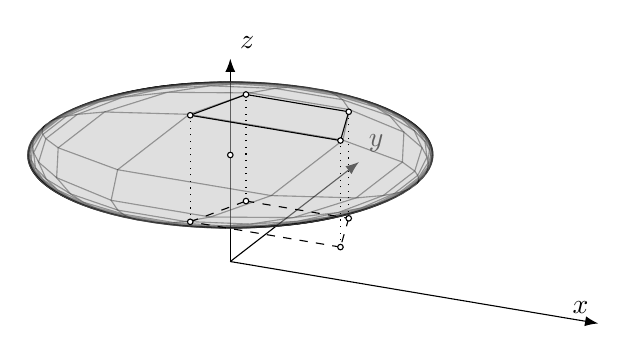
\begin{tikzpicture}[angle/.style={black,thick}]
\tikzmath{\a=0.05/sqrt(0.05*0.05+0.1*0.1);\k=1;\f=1;\u1=0;\v1=0;\u2=0;\v2=0;\u3=0;\v3=0;\u4=0;\v4=0;};
\a, \k,\u1,\v1,\u2,\v2,\u3,\v3,\u4,\v4,\f;
    %\pgfplotsset{ticks=none};
    \pgfplotsset{compat=1.12};
    \tikzset{>=latex} % for LaTeX arrow head
\begin{axis}
		[
		hide axis,clip=false,
		zmin=\k*0.5,
		zmax=\k,
			xmin=-\k,
		xmax=\k,
			ymin=-\k,
		ymax=\k,
		]
				%relevant points
	\coordinate (O) at ({ 0},{0},{0});%origin
	\coordinate (X) at ({ 2},{0},{0});%origin
	\coordinate (Y) at ({ 0},{1.5},{0});%origin
	\coordinate (Z) at ({ 0},{0},{0.4});%origin
	\draw[-Latex](O)--(X);
	\draw[-Latex](O)--(Y);
	\draw[-Latex](O)--(Z);
	\node[{anchor=south east}] at (X){$x$};
	\node[{anchor=south west}] at (Y){$y$};
	\node[{anchor=south west}] at (Z){$z$};
	\addplot3[surf,fill=gray!50,domain=-15:15,domain y=-15:15,samples=30,faceted color=black,mark=none, opacity=0.21,fill opacity = 0.5,thin]({x/sqrt(x*x*1+y*y+\f)},{y*\f/sqrt(x*x*1+y*y+\f)},{0.21});

			
 	\coordinate (Q) at ({ 0},{0},{0.21});%origin
\draw[fill=white](Q) circle(1pt)node[{anchor=north west}]{$$};; 	


	\tikzmath{\u1=0.5/sqrt(0.5*0.5+0.5*0.5+\f); \v1=0.5/sqrt(0.5*0.5+0.5*0.5+\f); 	};
	\coordinate (P0) at ({\u1},{\v1},{0.21});%origin
	\tikzmath{\u2=-0.5/sqrt(0.5*0.5+0.5*0.5+\f); \v2=0.5/sqrt(0.5*0.5+0.5*0.5+\f); 	};
	\coordinate (P1)at ({\u2},{\v2},{0.21});%origin
	\tikzmath{\u3=-0.5/sqrt(0.5*0.5+1.4*1.4+\f); \v3=1.4/sqrt(0.5*0.5+1.4*1.4+\f); 	};
	\coordinate (P2)at ({\u3},{\v3},{0.21});%origin
	\tikzmath{\u4=0.5/sqrt(0.5*0.5+1.4*1.4+\f); \v4=1.4/sqrt(0.5*0.5+1.4*1.4+\f); 	};
	\coordinate (P3)at ({\u4},{\v4},{0.21});%origin
	
		\coordinate (P0xy) at ({\u1},{\v1},{0});%origin
	\tikzmath{\u2=-0.5/sqrt(0.5*0.5+0.5*0.5+\f); \v2=0.5/sqrt(0.5*0.5+0.5*0.5+\f); 	};
	\coordinate (P1xy)at ({\u2},{\v2},{0});%origin
	\tikzmath{\u3=-0.5/sqrt(0.5*0.5+1.4*1.4+\f); \v3=1.4/sqrt(0.5*0.5+1.4*1.4+\f); 	};
	\coordinate (P2xy)at ({\u3},{\v3},{0});%origin
	\tikzmath{\u4=0.5/sqrt(0.5*0.5+1.4*1.4+\f); \v4=1.4/sqrt(0.5*0.5+1.4*1.4+\f); 	};
	\coordinate (P3xy)at ({\u4},{\v4},{0});%origin

	\draw[](P0)--(P1);
	\draw[](P1)--(P2);
	\draw[](P2)--(P3);
	\draw[](P3)--(P0);
	
	\draw[dashed](P0xy)--(P1xy);
	\draw[dashed](P1xy)--(P2xy);
	\draw[dashed](P2xy)--(P3xy);
	\draw[dashed](P3xy)--(P0xy);
	
		\draw[dotted](P0xy)--(P0);
	\draw[dotted](P1xy)--(P1);
	\draw[dotted](P2xy)--(P2);
	\draw[dotted](P3xy)--(P3);
	\draw[fill=white](P0) circle(1pt)node[{anchor=north west}]{$$};;
	\draw[fill=white](P1) circle(1pt)node[{anchor=north west}]{$$};;
	\draw[fill=white](P2) circle(1pt)node[{anchor=north west}]{$$};;
	\draw[fill=white](P3) circle(1pt)node[{anchor=north west}]{$$};;
	\draw[fill=white](P0xy) circle(1pt)node[{anchor=north west}]{$$};;
	\draw[fill=white](P1xy) circle(1pt)node[{anchor=north west}]{$$};;
	\draw[fill=white](P2xy) circle(1pt)node[{anchor=north west}]{$$};;
	\draw[fill=white](P3xy) circle(1pt)node[{anchor=north west}]{$$};;
	


		
\end{axis}
\end{tikzpicture}
=======
    \pgfplotsset{every axis/.append style={
view={120}{20},
%axis equal image,
    %clip=false,
    %xlabel=$x$, ylabel=$y$, zlabel=$z$,
    %axis lines=middle,
    colormap={whitered}{
        color(0cm)=(white);
        color(1cm)=(black!75!gray)
    }
    %y dir=reverse,
%    axis on top
            }}
            


            
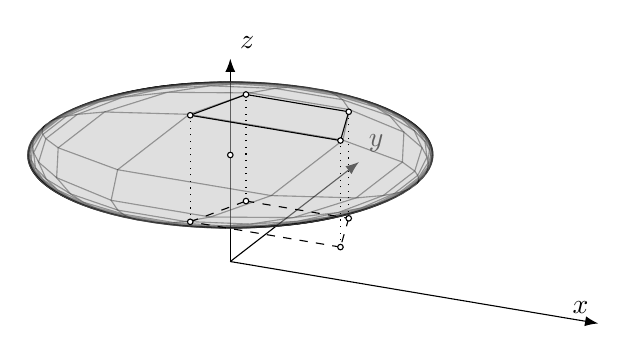
\begin{tikzpicture}[angle/.style={black,thick}]
\tikzmath{\a=0.05/sqrt(0.05*0.05+0.1*0.1);\k=1;\f=1;\u1=0;\v1=0;\u2=0;\v2=0;\u3=0;\v3=0;\u4=0;\v4=0;};
\a, \k,\u1,\v1,\u2,\v2,\u3,\v3,\u4,\v4,\f;
    %\pgfplotsset{ticks=none};
    \pgfplotsset{compat=1.12};
    \tikzset{>=latex} % for LaTeX arrow head
\begin{axis}
		[
		hide axis,clip=false,
		zmin=\k*0.5,
		zmax=\k,
			xmin=-\k,
		xmax=\k,
			ymin=-\k,
		ymax=\k,
		]
				%relevant points
	\coordinate (O) at ({ 0},{0},{0});%origin
	\coordinate (X) at ({ 2},{0},{0});%origin
	\coordinate (Y) at ({ 0},{1.5},{0});%origin
	\coordinate (Z) at ({ 0},{0},{0.4});%origin
	\draw[-Latex](O)--(X);
	\draw[-Latex](O)--(Y);
	\draw[-Latex](O)--(Z);
	\node[{anchor=south east}] at (X){$x$};
	\node[{anchor=south west}] at (Y){$y$};
	\node[{anchor=south west}] at (Z){$z$};
	\addplot3[surf,fill=gray!50,domain=-15:15,domain y=-15:15,samples=30,faceted color=black,mark=none, opacity=0.21,fill opacity = 0.5,thin]({x/sqrt(x*x*1+y*y+\f)},{y*\f/sqrt(x*x*1+y*y+\f)},{0.21});

			
 	\coordinate (Q) at ({ 0},{0},{0.21});%origin
\draw[fill=white](Q) circle(1pt)node[{anchor=north west}]{$$};; 	


	\tikzmath{\u1=0.5/sqrt(0.5*0.5+0.5*0.5+\f); \v1=0.5/sqrt(0.5*0.5+0.5*0.5+\f); 	};
	\coordinate (P0) at ({\u1},{\v1},{0.21});%origin
	\tikzmath{\u2=-0.5/sqrt(0.5*0.5+0.5*0.5+\f); \v2=0.5/sqrt(0.5*0.5+0.5*0.5+\f); 	};
	\coordinate (P1)at ({\u2},{\v2},{0.21});%origin
	\tikzmath{\u3=-0.5/sqrt(0.5*0.5+1.4*1.4+\f); \v3=1.4/sqrt(0.5*0.5+1.4*1.4+\f); 	};
	\coordinate (P2)at ({\u3},{\v3},{0.21});%origin
	\tikzmath{\u4=0.5/sqrt(0.5*0.5+1.4*1.4+\f); \v4=1.4/sqrt(0.5*0.5+1.4*1.4+\f); 	};
	\coordinate (P3)at ({\u4},{\v4},{0.21});%origin
	
		\coordinate (P0xy) at ({\u1},{\v1},{0});%origin
	\tikzmath{\u2=-0.5/sqrt(0.5*0.5+0.5*0.5+\f); \v2=0.5/sqrt(0.5*0.5+0.5*0.5+\f); 	};
	\coordinate (P1xy)at ({\u2},{\v2},{0});%origin
	\tikzmath{\u3=-0.5/sqrt(0.5*0.5+1.4*1.4+\f); \v3=1.4/sqrt(0.5*0.5+1.4*1.4+\f); 	};
	\coordinate (P2xy)at ({\u3},{\v3},{0});%origin
	\tikzmath{\u4=0.5/sqrt(0.5*0.5+1.4*1.4+\f); \v4=1.4/sqrt(0.5*0.5+1.4*1.4+\f); 	};
	\coordinate (P3xy)at ({\u4},{\v4},{0});%origin

	\draw[](P0)--(P1);
	\draw[](P1)--(P2);
	\draw[](P2)--(P3);
	\draw[](P3)--(P0);
	
	\draw[dashed](P0xy)--(P1xy);
	\draw[dashed](P1xy)--(P2xy);
	\draw[dashed](P2xy)--(P3xy);
	\draw[dashed](P3xy)--(P0xy);
	
		\draw[dotted](P0xy)--(P0);
	\draw[dotted](P1xy)--(P1);
	\draw[dotted](P2xy)--(P2);
	\draw[dotted](P3xy)--(P3);
	\draw[fill=white](P0) circle(1pt)node[{anchor=north west}]{$$};;
	\draw[fill=white](P1) circle(1pt)node[{anchor=north west}]{$$};;
	\draw[fill=white](P2) circle(1pt)node[{anchor=north west}]{$$};;
	\draw[fill=white](P3) circle(1pt)node[{anchor=north west}]{$$};;
	\draw[fill=white](P0xy) circle(1pt)node[{anchor=north west}]{$$};;
	\draw[fill=white](P1xy) circle(1pt)node[{anchor=north west}]{$$};;
	\draw[fill=white](P2xy) circle(1pt)node[{anchor=north west}]{$$};;
	\draw[fill=white](P3xy) circle(1pt)node[{anchor=north west}]{$$};;
	


		
\end{axis}
\end{tikzpicture}
>>>>>>> adfdd13a74863c750c19cd7f30af5a98907dce92
\caption{A disk defined as $S: \left\{\mathbb{R}^2\rightarrow \mathbb{R}^3: \ S(u,v)= \left(\frac{u}{\sqrt{u^2+v^2+C}},\ \frac{v}{\sqrt{u^2+v^2+C}}, \ 1\right)\right\}$}
\label{fig:fig_p257}
\end{figure}
\textbf{Conclusion:} The interpretation of  $d\tau_{(2)}^{k_1k_2}$ as the projection of a cell on a axis-plane, does not hold for every surface.
$$\blacklozenge$$
\newpage




\section{p263 - Exercise}
\begin{tcolorbox}
Using polar coordinates in Euclidean $3-$space find the volume of an infinitesimal cell whose edges are tangent to the coordinate curves. Obtain the volume of a sphere by integration.
\end{tcolorbox}
For polar spherical coordinates we have
\begin{align}
\left(a_{mn}\right)&= \left(\begin{array}{lll}
1&0&0\\
0&r^2&0\\
0&0&r^2\sin^2\theta
\end{array}\right)
\end{align}
giving
\begin{align}
\left|a_{mn}\right| &= r^4\sin^2\theta
\end{align}

and using as parameters the $x^k \equiv(r,\theta,\phi)$ as parameters for the parametric surface

we get 
\begin{align}
\left|d_{(s)}x^k\right| &= \left|\begin{array}{lll}
dr&0&0\\
0&d\theta&0\\
0&0&d\phi\\
\end{array}\right|\\
&= drd\theta d\phi
\end{align}

Using $\mathbf{7.405}$:
\begin{align}
dv_{(N)}^2&= \epsilon (a)\left|a_{mn}\right|\left|d_{(s)}x^k\right|^2\\
&= r^4\sin^2\theta\left( drd\theta d\phi\right)^2
\end{align}
getting for the volume of a sphere with radius $R$:
\begin{align}
V&=8 \int_{0}^{R}\int_{0}^{\frac{\pi}{2}}\int_{0}^{\frac{\pi}{2}}dv_{(N)}\\
&= 8 \int_{0}^{R}\int_{0}^{\frac{\pi}{2}}\int_{0}^{\frac{\pi}{2}}r^2\sin\theta dr d\theta d\phi\\
&= \frac{4}{3}\pi R^3
\end{align}
$$\blacklozenge$$
\newpage




\section{p265 - Exercise}
\begin{tcolorbox}
In the relativistic theory of finite, expanding universe, the following line element is adopted:
$$ds^2=R^2\left[dr^2+\sin^2 r\left(d\theta^2+\sin^2\theta d\phi^2\right)\right]-dt^2$$
where $R=R(t)$ is a function of the "time" $t$. the ranges of the coordinates may be taken to be $0\leq r\leq \pi, \ 0 \leq \theta \leq \pi,\ 0 \leq \phi< 2\pi,\ -\infty < t < + \infty$.\\
Find the total volume of "space", i.e., of the surface $t=$ constant, and show that it varies with the "time" $t$ as $R^3(t)$.
\end{tcolorbox}
For the considered metric, we have
\begin{align}
\left(a_{mn}\right)&= \left(\begin{array}{llll}
R^2&0&0&0\\
0&R^2\sin^2r&0&0\\
0&0&R^2\sin^2 r\sin^2\theta&0\\
0&0&0&-1
\end{array}\right)
\end{align}

Using as parameters the $x^k \equiv(r,\theta,\phi)$ as parameters for the parametric surface and using $\mathbf{7.409}:\quad b_{\alpha\beta}= a_{ks}\pdv{x^k}{y^{\alpha}}\pdv{x^s}{y^{\beta}} $, we get for the $3-$space $t=$ constant
\begin{align}
\left(b_{mn}\right)&= \left(\begin{array}{lll}
R^2&0&0\\
0&R^2\sin^2r&0\\
0&0&R^2\sin^2 r\sin^2\theta
\end{array}\right)
\end{align}
giving 
\begin{align}
\left|b_{mn}\right| &= R^6\sin^4 r\sin^2\theta
\end{align}
Using $\mathbf{7.413}$:
\begin{align}
dv_{(M)}^2&= \frac{\epsilon (b)}{M!}a_{k_1s_1}\dots a_{k_M s_M}d\tau_{(M)}^{k_1\dots k_M}d\tau_{(M)}^{s_1\dots s_M}\\
&= -\frac{1}{6}a_{k_1s_1}\dots a_{k_M s_M}d\tau_{(M)}^{k_1\dots k_M}d\tau_{(M)}^{s_1\dots s_M}\\
&= -\frac{6}{6}a_{11}a_{22}a_{33}\left(\underbrace{d\tau_{(M)}^{123}}_{=dr d\theta d\phi} \right)^2\\
&= -R^6\sin^4 r\sin^2\theta\left(dr d\theta d\phi \right)^2\\
\Rightarrow \quad dv_{(M)}&=R^3\sin^2 r\sin\theta dr d\theta d\phi
\end{align}


getting for the volume of "space"  with "radius" $R$:
\begin{align}
V&= \int_{0}^{\pi}\int_{0}^{\pi}\int_{0}^{2\pi}R^3\sin^2 r\sin\theta dr d\theta d\phi\\
&= 2 R^3\pi  \int_{0}^{R}\sin^2 r dr \underbrace{\int_{0}^{\pi}\sin\theta d\theta}_{=\left. -cos\theta\right|_0^{\pi}}\\
&= 4 R^3\pi  \underbrace{\int_{0}^{R}\sin^2 r dr}_{=\left.\half\left(\theta-\half\sin (2 r)\right)\right|_0^{\pi}}\\
&=2\pi^2 R^3  
\end{align}
(the integral in $(11)$ can be found by substituting $\sin^2 r = 1-\cos^2 r$ and  using the cosine sum of angles rule $\cos\left(\alpha+\beta\right) = \cos\alpha\cos\beta-\sin\alpha\sin\beta$ with $\alpha = \beta=r$).
$$\lozenge$$
In order to try to understand a little bit better what manifold is represented by the metric, let's use the trick to embed it in an higher dimensional space with en Euclidean metric.\\
Therefore let's use the following map:
\begin{align}
\left\{\begin{array}{l}
x=R\sin r\sin\theta\cos\phi\\
y=R\sin r\sin\theta\sin\phi\\
z=R\sin r\cos\theta\\
w=R\cos r
\end{array}\right.
\end{align}
then it's easy to see that
\begin{align}
ds_{(4)}^2 &=  dx^2+dy^2+dz^2+dw^2\\
&= R^2\left[dr^2+\sin^2 r\left(d\theta^2+\sin^2\theta d\phi^2\right)\right]
\end{align}
which is exactly the hypersurface we sought.
Now let's see what happens when we keep $\phi= 0 \text{ or } \pi$. Then $y=0$ and in fact we take a slice of the $4-space$ along the $xzw$ subspace, and can visualize this $3-$space as a sphere as represented by figure $7.5$(a). \\
We can also keep $r$ at a certain value. We get also a sphere as represented in figure $7.5$(b). Here the biggest possible sphere corresponds to $r=(2k+1)\frac{\pi}{2},\quad k=\{\dots,-1,0,1, \dots\}$ all other spheres having a smaller radius. When $r$ tends to $r=k\pi\quad k=\{\dots,-1,0,1, \dots\}$ the sphere shrinks to a point with coordinates $(0,0,0,\pm R)$.\\
Finally, keeping $\theta =k\pi,\quad k=\{\dots,-1,0,1, \dots\}$ we get a circle of radius $R$ situated in the $xw$ plane.

Remember that what we do here is just take 'slices' of a space. compare it to an Euclidean $3-$ space with a sphere: taking a slice e.g. parallel to the $xy$ plane will give us a circle, a point or an empty set while taking a one-dimensional slice along a line will give us 2, 1 or 0 point(s). 

\begin{figure}[H]%
    \centering
<<<<<<< HEAD
    \subfloat[]{
            


            
<<<<<<< HEAD
\begin{tikzpicture}[scale = 0.7,angle/.style={black,thick}]
=======
\begin{tikzpicture}[scale = 0.8,angle/.style={black,thick}]
>>>>>>> adfdd13a74863c750c19cd7f30af5a98907dce92

\pgfplotsset{every axis/.append style={
view={120}{20},
%axis equal image,
    %clip=false,
    %xlabel=$x$, ylabel=$y$, zlabel=$z$,
    %axis lines=middle,
    colormap={whitered}{
        color(0cm)=(white);
        color(1cm)=(black!75!gray)
    }
    %y dir=reverse,
%    axis on top
            }}

\tikzmath{\p=360;\a=1/sqrt(0.05*0.05+0.1*0.1);\k=3;\f=1;\u1=0;\v1=0;\u2=0;\v2=0;\u3=0;\v3=0;\u4=0;\v4=0;};
\p, \a, \k,\u1,\v1,\u2,\v2,\u3,\v3,\u4,\v4,\f;
    %\pgfplotsset{ticks=none};
    \pgfplotsset{compat=1.12};
    \tikzset{>=latex} % for LaTeX arrow head
\begin{axis}
		[
		axis equal image,
		hide axis,clip=false,
		zmin=-\k,
		zmax=\k,
			xmin=-\k,
		xmax=\k,
			ymin=-\k,
		ymax=\k,
		]
				%relevant points
	\coordinate (O) at ({ 0},{0},{0});%origin
	\coordinate (X) at ({4* \k},{0},{0});%origin
	\coordinate (Y) at ({ 0},{4*\k},{0});%origin
	\coordinate (Z) at ({ 0},{0},{4*\k});%origin
	\draw[-Latex](O)--(X);
	\draw[-Latex](O)--(Y);
	\draw[-Latex](O)--(Z);

	\addplot3[surf,fill=white!50,domain=0:\p,domain y=0:\p,samples=30,faceted color=gray!50,mark=none, opacity=0.21,fill opacity = 0.45,thin]({\a*sin(x)*cos(y)},{\a*sin(x)*sin(y)},{\a*cos(x)});
	\node[{anchor=south east}] at (X){$z$};
	\node[{anchor=south west}] at (Y){$x$};
	\node[{anchor=south west}] at (Z){$w$};
			
 \coordinate (Q) at ({ 0},{0},{0.0});%origin
\draw[fill=white](Q) circle(1pt)node[{anchor=north west}]{$$};; 	
 \coordinate (Qx) at ({\a*sin(0)*cos(0)},{\a*sin(0)*sin(0)},{\a*cos(0)});%origin
 \node[{anchor=south west}] at (Qx){$r=0, \theta =\pi$};
\draw[fill=white](Qx) circle(1pt)node[{anchor=north west}]{$$};; 
 \coordinate (Qz) at ({\a*sin(90)*cos(0)},{\a*sin(90)*sin(0)},{\a*cos(90)});%origin
 \node[{anchor=south west}] at (Qz){$r=\frac{\pi}{2}, \theta =0$};
\draw[fill=white](Qz) circle(1pt)node[{anchor=north west}]{$$};; 
 \coordinate (Qw) at ({\a*sin(90)*cos(90)},{\a*sin(90)*sin(90)},{\a*cos(90)});%origin
 \node[{anchor=south west}] at (Qw){$r=\frac{\pi}{2}, \theta =\frac{\pi}{2}$};
\draw[fill=white](Qw) circle(1pt)node[{anchor=north west}]{$$};; 


\draw[dashed] plot[variable=\x,domain=0:\p/4,samples=30,thick]({\a*sin(\x)*cos(0)},{\a*sin(\x)*sin(0)},{\a*cos(\x)});

\draw [postaction=decorate,decoration={markings,
    mark=at position 1 with {\arrow{Latex}}}] plot[variable=\x,domain=0:\p/9,samples=30,thick]({\a*sin(\x)*cos(60)},{\a*sin(\x)*sin(60)},{\a*cos(\x)});
 \coordinate (Pp) at ({\a*sin(\p/9)*cos(60)},{\a*sin(\p/9)*sin(60)},{\a*cos(\p/9)});
\draw[fill=white](Pp) circle(1.5pt)node[{anchor=west}]{$\phi =0$};; 

\draw [postaction=decorate,decoration={markings,
    mark=at position 1 with {\arrow{Latex}}}] plot[variable=\x,domain=0:\p/9,samples=30,thick]({\a*sin(\x)*cos(60)},{-\a*sin(\x)*sin(60)},{\a*cos(\x)});

\coordinate (Pn) at ({\a*sin(\p/9)*cos(60)},{-\a*sin(\p/9)*sin(60)},{\a*cos(\p/9)});
\draw[fill=white](Pn) circle(1.5pt)node[{anchor=east}]{$\phi =\pi$};; 

\draw[postaction=decorate,decoration={markings,
    mark=at position 1 with {\arrow{Latex}}}] plot[variable=\x,domain=0:60,samples=30,thick]({\a*sin(\p/9)*cos(\x)},{\a*sin(\p/9)*sin(\x)},{\a*cos(\p/9)});
\draw [postaction=decorate,decoration={markings,
    mark=at position 1 with {\arrow{Latex}}}] plot[variable=\x,domain=0:60,samples=30,thick]({\a*sin(\p/9)*cos(\x)},{-\a*sin(\p/9)*sin(\x)},{\a*cos(\p/9)});
 \coordinate (Pm) at ({\a*sin(\p/9)*cos(0)},{-\a*sin(\p/9)*sin(0)},{\a*cos(\p/9)});
\draw[fill=white](Pm) circle(1.5pt)node[{anchor= west}]{$$};; 

 \coordinate (Ta) at ({\a*sin(\p/9)*cos(30)},{\a*sin(\p/9)*sin(30)},{\a*cos(\p/9)});%origin
\draw[white,fill=white](Ta) circle(10pt)node[black]{$\theta$};; 

\coordinate (Tb) at ({\a*sin(\p/9)*cos(30)},{-\a*sin(\p/9)*sin(30)},{\a*cos(\p/9)});%origin
\draw[white,fill=white](Tb) circle(10pt)node[black]{$\theta$};; 

 \coordinate (Tc)  at ({\a*sin(\p/9/2)*cos(60)},{\a*sin(\p/9/2)*sin(60)},{\a*cos(\p/9/2)});
\draw[white,fill=white](Tc) circle(7pt)node[black]{$r$};

\coordinate (Td)  at ({\a*sin(\p/9/2)*cos(60)},{-\a*sin(\p/9/2)*sin(60)},{\a*cos(\p/9/2)});
\draw[white,fill=white](Td) circle(7pt)node[black]{$r$};



\coordinate (Te)  at ({\a*sin(55)*cos(0)},{\a*sin(55)*sin(0)},{\a*cos(55)});
\draw[white,fill=white](Te) circle(7pt)node[black]{$\theta=0$};

 
	\draw[-Latex](Qx)--(Z);
	\draw[-Latex](Qz)--(X);
	\draw[-Latex](Qw)--(Y);
\end{axis}
\end{tikzpicture}
}\\
    \subfloat[]{
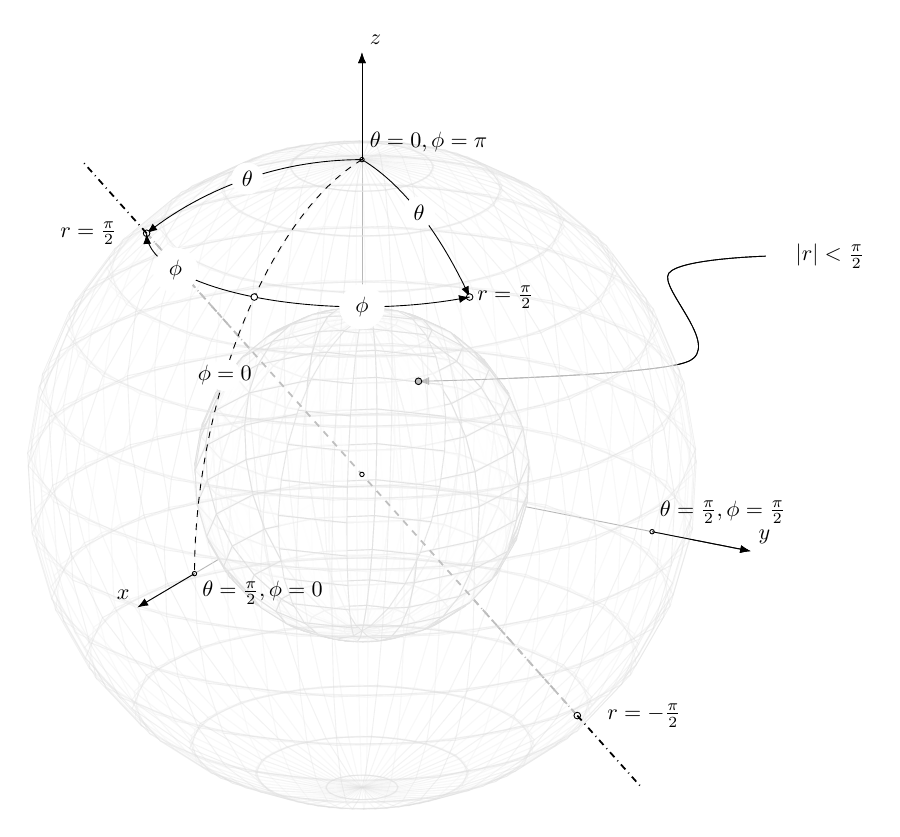
\begin{tikzpicture}[scale = 0.8,angle/.style={black,thick}]
\pgfplotsset{every axis/.append style={
view={120}{20},
axis equal image,
    %clip=false,
    %xlabel=$x$, ylabel=$y$, zlabel=$z$,
    %axis lines=middle,
    colormap={whitered}{
        color(0cm)=(white);
        color(1cm)=(black!75!gray)
    }
    %y dir=reverse,
%    axis on top
            }}
            
\tikzmath{\p=360;\a=1/sqrt(0.05*0.05+0.1*0.1);\k=3;\f=1;\u1=0;\v1=0;\u2=0;\v2=0;\u3=0;\v3=0;\u4=0;\v4=0;};
\p, \a, \k,\u1,\v1,\u2,\v2,\u3,\v3,\u4,\v4,\f;
    %\pgfplotsset{ticks=none};
    \pgfplotsset{compat=1.12};
    \tikzset{>=latex} % for LaTeX arrow head
\begin{axis}
		[axis equal image,
		hide axis,clip=false,
		zmin=-\k,
		zmax=\k,
			xmin=-\k,
		xmax=\k,
			ymin=-\k,
		ymax=\k,
		]
				%relevant points
	\coordinate (O) at ({ 0},{0},{0});%origin
	\coordinate (X) at ({4* \k},{0},{0});%origin
	\coordinate (Y) at ({ 0},{4*\k},{0});%origin
	\coordinate (Z) at ({ 0},{0},{4*\k});%origin
	\draw[-Latex](O)--(X);
	\draw[-Latex](O)--(Y);
	\draw[-Latex](O)--(Z);


\coordinate (Pn) at ({\a*sin(\p/9)*cos(60)},{-\a*sin(\p/9)*sin(60)},{\a*cos(\p/9)});
\coordinate (Pnn) at ({-\a*sin(\p/9)*cos(60)},{\a*sin(\p/9)*sin(60)},{-\a*cos(\p/9)});

\coordinate (Pnf) at ({1.3*\a*sin(\p/9)*cos(60)},{-1.3*\a*sin(\p/9)*sin(60)},{1.3*\a*cos(\p/9)});
\coordinate (Pnnf) at ({-1.3*\a*sin(\p/9)*cos(60)},{1.3*\a*sin(\p/9)*sin(60)},{-1.3*\a*cos(\p/9)});
\draw[dashdotted,thick](Pn)--(Pnn);
\coordinate (Pns) at ({1.05*\a*sin(\p/9)*cos(60)*sin(30)},{1.05*\a*sin(\p/9)*sin(60)*sin(30)},{1.05*\a*cos(\p/9)*sin(30)});
\coordinate (Pnsc) at ({\a*sin(\p/9)*cos(60)*1.5},{\a*sin(\p/9)*sin(60)*3},{\a*1.5*cos(\p/9)*1.});

	\draw[fill=black](Pns) circle(1.5pt)node[{anchor=west}]{$$};; 
	\draw[fill=white](Pnsc) circle(0pt)node[{anchor=west}]{$\quad |r|<\frac{\pi}{2}$};; 
	\draw []plot [smooth] coordinates {(Pnsc)  ({\a*sin(\p/9)*cos(60)*1.5},{0.8*\a*sin(\p/9)*sin(60)*3},{\a*cos(\p/9)*1.35})  ({\a*sin(\p/9)*cos(60)*1.5},{0.7*\a*sin(\p/9)*sin(60)*3.6},{\a*cos(\p/9)*1.}) (Pns)};

%draw surfaces
\addplot3[surf,fill=white!50,domain=0:\p,domain y=0:2*\p,samples=30,faceted color=gray!80,mark=none, opacity=0.8
	21,fill opacity = 0.65,thin]({\a*sin(1*30)*sin(x)*cos(y)},{\a*sin(1*30)*sin(x)*sin(y)},{\a*cos(x)*sin(1*30)});
\draw [-Latex]plot [smooth] coordinates {(Pnsc)  ({\a*sin(\p/9)*cos(60)*1.5},{0.8*\a*sin(\p/9)*sin(60)*3},{\a*cos(\p/9)*1.35})  ({\a*sin(\p/9)*cos(60)*1.5},{0.7*\a*sin(\p/9)*sin(60)*3.6},{\a*cos(\p/9)*1.}) (Pns)};

\addplot3[surf,fill=white!50,domain=0:\p,domain y=0:2*\p,samples=30,faceted color=gray!30,mark=none, opacity=0.21,fill opacity = 0.15,thin]({\a*sin(3*30)*sin(x)*cos(y)},{\a*sin(3*30)*sin(x)*sin(y)},{\a*cos(x)*sin(3*30)});

 \draw[dashed,thick, color = gray!50, opacity=1](Pn)--(Pnn);
	
	\node[{anchor=south east}] at (X){$x$};
	\node[{anchor=south west}] at (Y){$y$};
	\node[{anchor=south west}] at (Z){$z$};
			
 \coordinate (Q) at ({ 0},{0},{0.0});%origin
\draw[fill=white](Q) circle(1pt)node[{anchor=north west}]{$$};; 	
 \coordinate (Qx) at ({\a*sin(0)*cos(0)},{\a*sin(0)*sin(0)},{\a*cos(0)});%origin
 \node[{anchor=south west}] at (Qx){$\theta=0, \phi=\pi$};
\draw[fill=white](Qx) circle(1pt)node[{anchor=north west}]{$$};; 
 \coordinate (Qz) at ({\a*sin(90)*cos(0)},{\a*sin(90)*sin(0)},{\a*cos(90)});%origin
 \node[{anchor=north west}] at (Qz){$\theta=\frac{\pi}{2}, \phi =0$};
\draw[fill=white](Qz) circle(1pt)node[{anchor=north west}]{$$};; 
 \coordinate (Qw) at ({\a*sin(90)*cos(90)},{\a*sin(90)*sin(90)},{\a*cos(90)});%origin
 \node[{anchor=south west}] at (Qw){$\theta=\frac{\pi}{2}, \phi=\frac{\pi}{2}$};
\draw[fill=white](Qw) circle(1pt)node[{anchor=north west}]{$$};; 


\draw[dashed] plot[variable=\x,domain=0:\p/4,samples=30,thick]({\a*sin(\x)*cos(0)},{\a*sin(\x)*sin(0)},{\a*cos(\x)});

\draw [postaction=decorate,decoration={markings,
    mark=at position 1 with {\arrow{Latex}}}] plot[variable=\x,domain=0:\p/9,samples=30,thick]({\a*sin(\x)*cos(60)},{\a*sin(\x)*sin(60)},{\a*cos(\x)});
 \coordinate (Pp) at ({\a*sin(\p/9)*cos(60)},{\a*sin(\p/9)*sin(60)},{\a*cos(\p/9)});
\draw[fill=white](Pp) circle(1.5pt)node[{anchor=west}]{$r=\frac{\pi}{2}$};; 

\draw [postaction=decorate,decoration={markings,
    mark=at position 1 with {\arrow{Latex}}}] plot[variable=\x,domain=0:\p/9,samples=30,thick]({\a*sin(\x)*cos(60)},{-\a*sin(\x)*sin(60)},{\a*cos(\x)});

\draw[fill=white](Pn) circle(1.5pt)node[{anchor=east}]{$r=\frac{\pi}{2} \quad$};; 
\draw[fill=white](Pnn) circle(1.5pt)node[{anchor=west}]{$\quad r=-\frac{\pi}{2}$};; 



\draw[postaction=decorate,decoration={markings,
    mark=at position 1 with {\arrow{Latex}}}] plot[variable=\x,domain=0:60,samples=30,thick]({\a*sin(\p/9)*cos(\x)},{\a*sin(\p/9)*sin(\x)},{\a*cos(\p/9)});
\draw [postaction=decorate,decoration={markings,
    mark=at position 1 with {\arrow{Latex}}}] plot[variable=\x,domain=0:60,samples=30,thick]({\a*sin(\p/9)*cos(\x)},{-\a*sin(\p/9)*sin(\x)},{\a*cos(\p/9)});
 \coordinate (Pm) at ({\a*sin(\p/9)*cos(0)},{-\a*sin(\p/9)*sin(0)},{\a*cos(\p/9)});
\draw[fill=white](Pm) circle(1.5pt)node[{anchor= west}]{$$};; 

 \coordinate (Ta) at ({\a*sin(\p/9)*cos(30)},{\a*sin(\p/9)*sin(30)},{\a*cos(\p/9)});%origin
\draw[white,fill=white](Ta) circle(10pt)node[black]{$\phi$};; 

\coordinate (Tb) at ({\a*sin(\p/9)*cos(30)},{-\a*sin(\p/9)*sin(30)},{\a*cos(\p/9)});%origin
\draw[white,fill=white](Tb) circle(10pt)node[black]{$\phi$};; 

 \coordinate (Tc)  at ({\a*sin(\p/9/2)*cos(60)},{\a*sin(\p/9/2)*sin(60)},{\a*cos(\p/9/2)});
\draw[white,fill=white](Tc) circle(7pt)node[black]{$\theta$};

\coordinate (Td)  at ({\a*sin(\p/9/2)*cos(60)},{-\a*sin(\p/9/2)*sin(60)},{\a*cos(\p/9/2)});
\draw[white,fill=white](Td) circle(7pt)node[black]{$\theta$};



\coordinate (Te)  at ({\a*sin(55)*cos(0)},{\a*sin(55)*sin(0)},{\a*cos(55)});
\draw[white,fill=white](Te) circle(7pt)node[black]{$\phi=0$};

 \draw[dashdotted,thick](Pn)--(Pnf);

\draw[dashdotted,thick](Pnn)--(Pnnf);
	\draw[-Latex](Qx)--(Z);
	\draw[-Latex](Qz)--(X);
	\draw[-Latex](Qw)--(Y);
	\draw[fill=gray!50](Pns) circle(1.5pt)node[{anchor=west}]{$$};;

\end{axis}
\end{tikzpicture}}
=======
    \subfloat[]{
            


            
<<<<<<< HEAD
\begin{tikzpicture}[scale = 0.7,angle/.style={black,thick}]
=======
\begin{tikzpicture}[scale = 0.8,angle/.style={black,thick}]
>>>>>>> adfdd13a74863c750c19cd7f30af5a98907dce92

\pgfplotsset{every axis/.append style={
view={120}{20},
%axis equal image,
    %clip=false,
    %xlabel=$x$, ylabel=$y$, zlabel=$z$,
    %axis lines=middle,
    colormap={whitered}{
        color(0cm)=(white);
        color(1cm)=(black!75!gray)
    }
    %y dir=reverse,
%    axis on top
            }}

\tikzmath{\p=360;\a=1/sqrt(0.05*0.05+0.1*0.1);\k=3;\f=1;\u1=0;\v1=0;\u2=0;\v2=0;\u3=0;\v3=0;\u4=0;\v4=0;};
\p, \a, \k,\u1,\v1,\u2,\v2,\u3,\v3,\u4,\v4,\f;
    %\pgfplotsset{ticks=none};
    \pgfplotsset{compat=1.12};
    \tikzset{>=latex} % for LaTeX arrow head
\begin{axis}
		[
		axis equal image,
		hide axis,clip=false,
		zmin=-\k,
		zmax=\k,
			xmin=-\k,
		xmax=\k,
			ymin=-\k,
		ymax=\k,
		]
				%relevant points
	\coordinate (O) at ({ 0},{0},{0});%origin
	\coordinate (X) at ({4* \k},{0},{0});%origin
	\coordinate (Y) at ({ 0},{4*\k},{0});%origin
	\coordinate (Z) at ({ 0},{0},{4*\k});%origin
	\draw[-Latex](O)--(X);
	\draw[-Latex](O)--(Y);
	\draw[-Latex](O)--(Z);

	\addplot3[surf,fill=white!50,domain=0:\p,domain y=0:\p,samples=30,faceted color=gray!50,mark=none, opacity=0.21,fill opacity = 0.45,thin]({\a*sin(x)*cos(y)},{\a*sin(x)*sin(y)},{\a*cos(x)});
	\node[{anchor=south east}] at (X){$z$};
	\node[{anchor=south west}] at (Y){$x$};
	\node[{anchor=south west}] at (Z){$w$};
			
 \coordinate (Q) at ({ 0},{0},{0.0});%origin
\draw[fill=white](Q) circle(1pt)node[{anchor=north west}]{$$};; 	
 \coordinate (Qx) at ({\a*sin(0)*cos(0)},{\a*sin(0)*sin(0)},{\a*cos(0)});%origin
 \node[{anchor=south west}] at (Qx){$r=0, \theta =\pi$};
\draw[fill=white](Qx) circle(1pt)node[{anchor=north west}]{$$};; 
 \coordinate (Qz) at ({\a*sin(90)*cos(0)},{\a*sin(90)*sin(0)},{\a*cos(90)});%origin
 \node[{anchor=south west}] at (Qz){$r=\frac{\pi}{2}, \theta =0$};
\draw[fill=white](Qz) circle(1pt)node[{anchor=north west}]{$$};; 
 \coordinate (Qw) at ({\a*sin(90)*cos(90)},{\a*sin(90)*sin(90)},{\a*cos(90)});%origin
 \node[{anchor=south west}] at (Qw){$r=\frac{\pi}{2}, \theta =\frac{\pi}{2}$};
\draw[fill=white](Qw) circle(1pt)node[{anchor=north west}]{$$};; 


\draw[dashed] plot[variable=\x,domain=0:\p/4,samples=30,thick]({\a*sin(\x)*cos(0)},{\a*sin(\x)*sin(0)},{\a*cos(\x)});

\draw [postaction=decorate,decoration={markings,
    mark=at position 1 with {\arrow{Latex}}}] plot[variable=\x,domain=0:\p/9,samples=30,thick]({\a*sin(\x)*cos(60)},{\a*sin(\x)*sin(60)},{\a*cos(\x)});
 \coordinate (Pp) at ({\a*sin(\p/9)*cos(60)},{\a*sin(\p/9)*sin(60)},{\a*cos(\p/9)});
\draw[fill=white](Pp) circle(1.5pt)node[{anchor=west}]{$\phi =0$};; 

\draw [postaction=decorate,decoration={markings,
    mark=at position 1 with {\arrow{Latex}}}] plot[variable=\x,domain=0:\p/9,samples=30,thick]({\a*sin(\x)*cos(60)},{-\a*sin(\x)*sin(60)},{\a*cos(\x)});

\coordinate (Pn) at ({\a*sin(\p/9)*cos(60)},{-\a*sin(\p/9)*sin(60)},{\a*cos(\p/9)});
\draw[fill=white](Pn) circle(1.5pt)node[{anchor=east}]{$\phi =\pi$};; 

\draw[postaction=decorate,decoration={markings,
    mark=at position 1 with {\arrow{Latex}}}] plot[variable=\x,domain=0:60,samples=30,thick]({\a*sin(\p/9)*cos(\x)},{\a*sin(\p/9)*sin(\x)},{\a*cos(\p/9)});
\draw [postaction=decorate,decoration={markings,
    mark=at position 1 with {\arrow{Latex}}}] plot[variable=\x,domain=0:60,samples=30,thick]({\a*sin(\p/9)*cos(\x)},{-\a*sin(\p/9)*sin(\x)},{\a*cos(\p/9)});
 \coordinate (Pm) at ({\a*sin(\p/9)*cos(0)},{-\a*sin(\p/9)*sin(0)},{\a*cos(\p/9)});
\draw[fill=white](Pm) circle(1.5pt)node[{anchor= west}]{$$};; 

 \coordinate (Ta) at ({\a*sin(\p/9)*cos(30)},{\a*sin(\p/9)*sin(30)},{\a*cos(\p/9)});%origin
\draw[white,fill=white](Ta) circle(10pt)node[black]{$\theta$};; 

\coordinate (Tb) at ({\a*sin(\p/9)*cos(30)},{-\a*sin(\p/9)*sin(30)},{\a*cos(\p/9)});%origin
\draw[white,fill=white](Tb) circle(10pt)node[black]{$\theta$};; 

 \coordinate (Tc)  at ({\a*sin(\p/9/2)*cos(60)},{\a*sin(\p/9/2)*sin(60)},{\a*cos(\p/9/2)});
\draw[white,fill=white](Tc) circle(7pt)node[black]{$r$};

\coordinate (Td)  at ({\a*sin(\p/9/2)*cos(60)},{-\a*sin(\p/9/2)*sin(60)},{\a*cos(\p/9/2)});
\draw[white,fill=white](Td) circle(7pt)node[black]{$r$};



\coordinate (Te)  at ({\a*sin(55)*cos(0)},{\a*sin(55)*sin(0)},{\a*cos(55)});
\draw[white,fill=white](Te) circle(7pt)node[black]{$\theta=0$};

 
	\draw[-Latex](Qx)--(Z);
	\draw[-Latex](Qz)--(X);
	\draw[-Latex](Qw)--(Y);
\end{axis}
\end{tikzpicture}
}\\
    \subfloat[]{
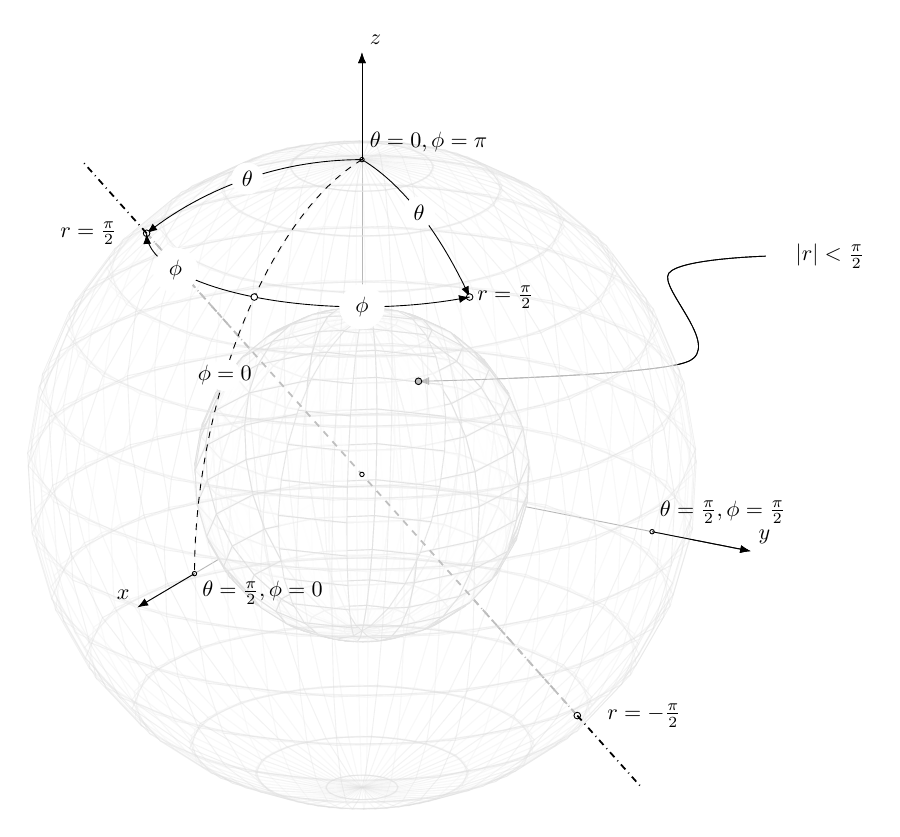
\begin{tikzpicture}[scale = 0.8,angle/.style={black,thick}]
\pgfplotsset{every axis/.append style={
view={120}{20},
axis equal image,
    %clip=false,
    %xlabel=$x$, ylabel=$y$, zlabel=$z$,
    %axis lines=middle,
    colormap={whitered}{
        color(0cm)=(white);
        color(1cm)=(black!75!gray)
    }
    %y dir=reverse,
%    axis on top
            }}
            
\tikzmath{\p=360;\a=1/sqrt(0.05*0.05+0.1*0.1);\k=3;\f=1;\u1=0;\v1=0;\u2=0;\v2=0;\u3=0;\v3=0;\u4=0;\v4=0;};
\p, \a, \k,\u1,\v1,\u2,\v2,\u3,\v3,\u4,\v4,\f;
    %\pgfplotsset{ticks=none};
    \pgfplotsset{compat=1.12};
    \tikzset{>=latex} % for LaTeX arrow head
\begin{axis}
		[axis equal image,
		hide axis,clip=false,
		zmin=-\k,
		zmax=\k,
			xmin=-\k,
		xmax=\k,
			ymin=-\k,
		ymax=\k,
		]
				%relevant points
	\coordinate (O) at ({ 0},{0},{0});%origin
	\coordinate (X) at ({4* \k},{0},{0});%origin
	\coordinate (Y) at ({ 0},{4*\k},{0});%origin
	\coordinate (Z) at ({ 0},{0},{4*\k});%origin
	\draw[-Latex](O)--(X);
	\draw[-Latex](O)--(Y);
	\draw[-Latex](O)--(Z);


\coordinate (Pn) at ({\a*sin(\p/9)*cos(60)},{-\a*sin(\p/9)*sin(60)},{\a*cos(\p/9)});
\coordinate (Pnn) at ({-\a*sin(\p/9)*cos(60)},{\a*sin(\p/9)*sin(60)},{-\a*cos(\p/9)});

\coordinate (Pnf) at ({1.3*\a*sin(\p/9)*cos(60)},{-1.3*\a*sin(\p/9)*sin(60)},{1.3*\a*cos(\p/9)});
\coordinate (Pnnf) at ({-1.3*\a*sin(\p/9)*cos(60)},{1.3*\a*sin(\p/9)*sin(60)},{-1.3*\a*cos(\p/9)});
\draw[dashdotted,thick](Pn)--(Pnn);
\coordinate (Pns) at ({1.05*\a*sin(\p/9)*cos(60)*sin(30)},{1.05*\a*sin(\p/9)*sin(60)*sin(30)},{1.05*\a*cos(\p/9)*sin(30)});
\coordinate (Pnsc) at ({\a*sin(\p/9)*cos(60)*1.5},{\a*sin(\p/9)*sin(60)*3},{\a*1.5*cos(\p/9)*1.});

	\draw[fill=black](Pns) circle(1.5pt)node[{anchor=west}]{$$};; 
	\draw[fill=white](Pnsc) circle(0pt)node[{anchor=west}]{$\quad |r|<\frac{\pi}{2}$};; 
	\draw []plot [smooth] coordinates {(Pnsc)  ({\a*sin(\p/9)*cos(60)*1.5},{0.8*\a*sin(\p/9)*sin(60)*3},{\a*cos(\p/9)*1.35})  ({\a*sin(\p/9)*cos(60)*1.5},{0.7*\a*sin(\p/9)*sin(60)*3.6},{\a*cos(\p/9)*1.}) (Pns)};

%draw surfaces
\addplot3[surf,fill=white!50,domain=0:\p,domain y=0:2*\p,samples=30,faceted color=gray!80,mark=none, opacity=0.8
	21,fill opacity = 0.65,thin]({\a*sin(1*30)*sin(x)*cos(y)},{\a*sin(1*30)*sin(x)*sin(y)},{\a*cos(x)*sin(1*30)});
\draw [-Latex]plot [smooth] coordinates {(Pnsc)  ({\a*sin(\p/9)*cos(60)*1.5},{0.8*\a*sin(\p/9)*sin(60)*3},{\a*cos(\p/9)*1.35})  ({\a*sin(\p/9)*cos(60)*1.5},{0.7*\a*sin(\p/9)*sin(60)*3.6},{\a*cos(\p/9)*1.}) (Pns)};

\addplot3[surf,fill=white!50,domain=0:\p,domain y=0:2*\p,samples=30,faceted color=gray!30,mark=none, opacity=0.21,fill opacity = 0.15,thin]({\a*sin(3*30)*sin(x)*cos(y)},{\a*sin(3*30)*sin(x)*sin(y)},{\a*cos(x)*sin(3*30)});

 \draw[dashed,thick, color = gray!50, opacity=1](Pn)--(Pnn);
	
	\node[{anchor=south east}] at (X){$x$};
	\node[{anchor=south west}] at (Y){$y$};
	\node[{anchor=south west}] at (Z){$z$};
			
 \coordinate (Q) at ({ 0},{0},{0.0});%origin
\draw[fill=white](Q) circle(1pt)node[{anchor=north west}]{$$};; 	
 \coordinate (Qx) at ({\a*sin(0)*cos(0)},{\a*sin(0)*sin(0)},{\a*cos(0)});%origin
 \node[{anchor=south west}] at (Qx){$\theta=0, \phi=\pi$};
\draw[fill=white](Qx) circle(1pt)node[{anchor=north west}]{$$};; 
 \coordinate (Qz) at ({\a*sin(90)*cos(0)},{\a*sin(90)*sin(0)},{\a*cos(90)});%origin
 \node[{anchor=north west}] at (Qz){$\theta=\frac{\pi}{2}, \phi =0$};
\draw[fill=white](Qz) circle(1pt)node[{anchor=north west}]{$$};; 
 \coordinate (Qw) at ({\a*sin(90)*cos(90)},{\a*sin(90)*sin(90)},{\a*cos(90)});%origin
 \node[{anchor=south west}] at (Qw){$\theta=\frac{\pi}{2}, \phi=\frac{\pi}{2}$};
\draw[fill=white](Qw) circle(1pt)node[{anchor=north west}]{$$};; 


\draw[dashed] plot[variable=\x,domain=0:\p/4,samples=30,thick]({\a*sin(\x)*cos(0)},{\a*sin(\x)*sin(0)},{\a*cos(\x)});

\draw [postaction=decorate,decoration={markings,
    mark=at position 1 with {\arrow{Latex}}}] plot[variable=\x,domain=0:\p/9,samples=30,thick]({\a*sin(\x)*cos(60)},{\a*sin(\x)*sin(60)},{\a*cos(\x)});
 \coordinate (Pp) at ({\a*sin(\p/9)*cos(60)},{\a*sin(\p/9)*sin(60)},{\a*cos(\p/9)});
\draw[fill=white](Pp) circle(1.5pt)node[{anchor=west}]{$r=\frac{\pi}{2}$};; 

\draw [postaction=decorate,decoration={markings,
    mark=at position 1 with {\arrow{Latex}}}] plot[variable=\x,domain=0:\p/9,samples=30,thick]({\a*sin(\x)*cos(60)},{-\a*sin(\x)*sin(60)},{\a*cos(\x)});

\draw[fill=white](Pn) circle(1.5pt)node[{anchor=east}]{$r=\frac{\pi}{2} \quad$};; 
\draw[fill=white](Pnn) circle(1.5pt)node[{anchor=west}]{$\quad r=-\frac{\pi}{2}$};; 



\draw[postaction=decorate,decoration={markings,
    mark=at position 1 with {\arrow{Latex}}}] plot[variable=\x,domain=0:60,samples=30,thick]({\a*sin(\p/9)*cos(\x)},{\a*sin(\p/9)*sin(\x)},{\a*cos(\p/9)});
\draw [postaction=decorate,decoration={markings,
    mark=at position 1 with {\arrow{Latex}}}] plot[variable=\x,domain=0:60,samples=30,thick]({\a*sin(\p/9)*cos(\x)},{-\a*sin(\p/9)*sin(\x)},{\a*cos(\p/9)});
 \coordinate (Pm) at ({\a*sin(\p/9)*cos(0)},{-\a*sin(\p/9)*sin(0)},{\a*cos(\p/9)});
\draw[fill=white](Pm) circle(1.5pt)node[{anchor= west}]{$$};; 

 \coordinate (Ta) at ({\a*sin(\p/9)*cos(30)},{\a*sin(\p/9)*sin(30)},{\a*cos(\p/9)});%origin
\draw[white,fill=white](Ta) circle(10pt)node[black]{$\phi$};; 

\coordinate (Tb) at ({\a*sin(\p/9)*cos(30)},{-\a*sin(\p/9)*sin(30)},{\a*cos(\p/9)});%origin
\draw[white,fill=white](Tb) circle(10pt)node[black]{$\phi$};; 

 \coordinate (Tc)  at ({\a*sin(\p/9/2)*cos(60)},{\a*sin(\p/9/2)*sin(60)},{\a*cos(\p/9/2)});
\draw[white,fill=white](Tc) circle(7pt)node[black]{$\theta$};

\coordinate (Td)  at ({\a*sin(\p/9/2)*cos(60)},{-\a*sin(\p/9/2)*sin(60)},{\a*cos(\p/9/2)});
\draw[white,fill=white](Td) circle(7pt)node[black]{$\theta$};



\coordinate (Te)  at ({\a*sin(55)*cos(0)},{\a*sin(55)*sin(0)},{\a*cos(55)});
\draw[white,fill=white](Te) circle(7pt)node[black]{$\phi=0$};

 \draw[dashdotted,thick](Pn)--(Pnf);

\draw[dashdotted,thick](Pnn)--(Pnnf);
	\draw[-Latex](Qx)--(Z);
	\draw[-Latex](Qz)--(X);
	\draw[-Latex](Qw)--(Y);
	\draw[fill=gray!50](Pns) circle(1.5pt)node[{anchor=west}]{$$};;

\end{axis}
\end{tikzpicture}}
>>>>>>> adfdd13a74863c750c19cd7f30af5a98907dce92
\caption{Manifold with $ds^2=R^2\left[dr^2+\sin^2 r\left(d\theta^2+\sin^2\theta d\phi^2\right)\right]$ metric, embedded in an Euclidean $4-$space}
\label{fig:fig_p265}
\end{figure}
$$\blacklozenge$$
\newpage



\section{p268 - Clarification }
\begin{tcolorbox}
Since $\pdv{T_k}{x^s}$ differs from the tensor $\half\left(T_{k,s}-T_{s,k}\right)$ by an expression symmetric in $k, \ s$ and $d\tau_{(2)}^{ks}$ is an absolute tensor, skew-symmetric in these suffixes, it follows that the integrand on the left is an invariant.
\end{tcolorbox}
Let's express $\mathbf{7.504}$ in curvilinear coordinates, equipped with metric
\begin{align}
\int_{R_2}T_{k|s}d\tau_{(2)}^{ks} = \int_{R_1}T_{r}d\tau_{(1)}^{r}
\end{align}
Obviously we have 
\begin{align}
T_{k|s}&= \half\left(T_{k|s}-T_{s|k}\right)+\half\left(T_{k|s}+T_{s|k}\right)
\end{align}
Let's put $A_{ks}= \half\left(T_{k|s}-T_{s|k}\right)$ and $B_{ks}= \half\left(T_{k|s}+T_{s|k}\right)$.\\
$A_{ks}$ is skew-symmetric, while $B_{ks}$ is symmetric.
Note also that $A_{ks}$ reduces to $A_{ks}=\half\left(T_{k,s}-T_{s,k}\right)$ as the Christoffel symbols vanish in this expression, leaving only the partial differentials and hence, independent of a metric. 
So the integrand  on the left side becomes
\begin{align}
T_{k|s}d\tau_{(2)}^{ks} &= A_{ks}d\tau_{(2)}^{ks}+B_{ks}d\tau_{(2)}^{ks}\\
\Rightarrow\quad T_{k|s}d\tau_{(2)}^{ks} &= A_{ks}d\tau_{(2)}^{ks}-B_{ks}d\tau_{(2)}^{sk}\\
&= A_{ks}d\tau_{(2)}^{ks}-B_{sk}d\tau_{(2)}^{sk}\\
\text{(3)+(5)}\quad\Rightarrow\quad T_{k|s}d\tau_{(2)}^{ks} &= A_{ks}d\tau_{(2)}^{ks}
\end{align}
We note that both $A_{ks}$ and $d\tau_{(2)}^{ks}$ are tensors, independent of the  metric defined, and thus $A_{ks}d\tau_{(2)}^{ks}$ is an invariant of order $0$. 
$$\blacklozenge$$
\newpage


\section{p274 - Exercise }
\begin{tcolorbox}
Due to the skew-symmetry of $d\tau_{(M)}^{k_1\dots k_M}$, the integrand on the left-hand side is also an invariant. This may be proved in a few lines, preferably with the use of the compressed notation of $1.7$; the proof is left as an exercise for the reader.
\end{tcolorbox}
We will use the indices $i,j$ for the transformed tensor components and $p,q$ for the original components.
We have 
\begin{align}
T^{'}_{i_1 \dots i_{M-1}}&= T^{}_{p_1 \dots p_{M-1}}X^{p_1}_{i_1}\dots X^{p_{M-1}}_{i_{M-1}}\\
\Rightarrow \quad T^{'}_{i_1 \dots i_{M-1},i_M}&= T^{}_{p_1 \dots p_{M-1},i_M}X^{p_1}_{i_1}\dots X^{p_{M-1}}_{i_{M-1}}+T^{}_{p_1 \dots p_{M-1}}\left(X^{p_1}_{i_1}\dots X^{p_{M-1}}_{i_{M-1}}\right)_{,i_M}\\
&= T^{}_{p_1 \dots p_{M-1},p_M}X^{p_1}_{i_1}\dots X^{p_{M-1}}_{i_{M-1}}X^{p_{M}}_{i_{M}}+T^{}_{p_1 \dots p_{M-1}}\left(X^{p_1}_{i_1}\dots X^{p_{M-1}}_{i_{M-1}}\right)_{,i_M}\
\end{align} 
and 
\begin{align}
d\tau_{(M)}^{'i_1 \dots i_{M}}&= d\tau_{(M)}^{s_1 \dots s_{M}}X^{i_1}_{s_1}\dots X^{i_{M}}_{s_{M}}
\end{align}
This gives 
\begin{align}
 T^{'}_{i_1 \dots i_{M-1},i_M}d\tau_{(M)}^{'i_1 \dots i_{M}}&=\left\{\begin{array}{l}T^{}_{p_1 \dots p_{M-1},p_M}X^{p_1}_{i_1}\dots X^{p_{M-1}}_{i_{M-1}}X^{p_{M}}_{i_{M}}d\tau_{(M)}^{s_1 \dots s_{M}}X^{i_1}_{s_1}\dots X^{i_{M}}_{s_{M}}\\\\
 +\underbrace{T^{}_{p_1 \dots p_{M-1}}\left(X^{p_1}_{i_1}\dots X^{p_{M-1}}_{i_{M-1}}\right)_{,i_M}d\tau_{(M)}^{s_1 \dots s_{M}}X^{i_1}_{s_1}\dots X^{i_{M}}_{s_{M}}}_{=0} 
 \end{array}\right.\\
 &=T^{}_{p_1 \dots p_{M-1},p_M}X^{p_1}_{s_1}\dots X^{p_{M-1}}_{s_{M-1}}X^{p_{M}}_{s_{M}}d\tau_{(M)}^{s_1 \dots s_{M}}\\
  &=T^{}_{p_1 \dots p_{M-1},p_M}\delta^{p_1}_{s_1}\dots \delta^{p_{M-1}}_{s_{M-1}}\delta^{p_{M}}_{s_{M}}d\tau_{(M)}^{s_1 \dots s_{M}}\\
   &=T^{}_{s_1 \dots s_{M-1},s_M}d\tau_{(M)}^{s_1 \dots s_{M}}
\end{align}
The term $ T^{}_{p_1 \dots p_{M-1}}\left(X^{p_1}_{i_1}\dots X^{p_{M-1}}_{i_{M-1}}\right)_{,i_M}d\tau_{(M)}^{s_1 \dots s_{M}}X^{i_1}_{s_1}\dots X^{i_{M}}_{s_{M}}$ in $ (5)$  is zero. Indeed, rewriting this as : 
\begin{align} T^{}_{p_1 \dots p_{M-1}}\left(X^{p_1}_{i_1}\dots X^{p_{M-1}}_{i_{M-1}}\right)_{,p_M}X^{p_M}_{i_M}d\tau_{(M)}^{s_1 \dots s_{M}}X^{i_1}_{s_1}\dots X^{i_{M}}_{s_{M}}
\end{align}
The terms in brackets are zero as they are of the form
\begin{align}
\dots + X^{p_1}_{i_1}\dots \underbrace{\pdv[2]{x^{p_{m}}}{x^{p_{M}}}{x^{'i_{m}}}}_{= \pdv{\delta^{p_m}_{p_M}}{x^{'i_{m}}}=0}\dots X^{p_{M-1}}_{i_{M-1}}+\dots 
\end{align} 
From $(8)$ we conclude that the integrand is indeed an invariant.
$$\blacklozenge$$
\newpage

\section{p275 - Exercise }
\begin{tcolorbox}
The skew-symmetric part of a tensor $T_{k_1\dots k_M}$ is defined as  
$$ T_{\left [k_1 \dots k_M\right ]}= \left(M!\right)^{-1}\delta_{k_1 \dots k_M}^{s_1 \dots s_M} T_{s_1\dots s_M}$$
Show that the left-hand side of equation $\mathbf{7.525}$ is unchanged if $T_{k_1\dots k_M}$ is replace by its skew-symmetric part. Show that the same is true for the right-hand side.
\end{tcolorbox}
The integrand of the left-hand side of $\mathbf{7.525}$ is
\begin{align}
T_{k_1\dots k_{M-1},k_M}d\tau_{(M)}^{k_1\dots k_M}
\end{align}
replacing the tensor with it's skew-symmetric part gives
\begin{align}
T_{\left [k_1 \dots k_{M-1}\right ],k_M}d\tau_{(M)}^{k_1\dots k_M}&= \frac{1}{\left(M-1\right)!}\delta_{k_1 \dots k_{M-1}}^{s_1 \dots s_{M-1}} T_{s_1\dots s_{M-1},k_M}d\tau_{(M)}^{k_1\dots k_M}\\
&= \frac{1}{\left(M-1\right)!}\delta_{k_1 \dots k_{M-1}}^{s_1 \dots s_{M-1}} \delta^{s_M}_{k_M}T_{s_1\dots s_{M-1},s_M}d\tau_{(M)}^{k_1\dots k_M}\\
&= \frac{1}{\left(M-1\right)!}\delta_{k_1 \dots k_{M-1}}^{s_1 \dots s_{M-1}} T_{s_1\dots s_{M-1},s_M}d\tau_{(M)}^{k_1\dots k_{M-1}s_M}\\
&=T_{s_1\dots s_{M-1},s_M} \frac{1}{\left(M-1\right)!}\left(\delta_{k_1 \dots k_{M-1}}^{s_1 \dots s_{M-1}} d\tau_{(M)}^{k_1\dots k_{M-1}s_M}\right)\\
\end{align}
The terms in the brackets can be reduced to $\left(M-1\right)! d\tau_{(M)}^{s_1\dots s_{M-1}s_M}$. Indeed, the number of choices in choosing the $k_1,\dots k_{M-1}$ are restricted to $M-1$ choices, due to the skew-symmetry of $d\tau_{(M)}^{k_1\dots k_{M-1}s_M}$ (choosing a $k_i= s_M$ would result in a zero value for $d\tau_{(M)}^{k_1\dots k_{M-1}s_M}$). So, in total there will be $ \left(M-1\right)!$ terms and due to the skew-symmetry of $d\tau_{(M)}^{k_1\dots k_{M-1}s_M}$  a change in sign of $\delta_{k_1 \dots k_{M-1}}^{s_1 \dots s_{M-1}}$ will also result in a change of sign in $d\tau_{(M)}^{k_1\dots k_{M-1}s_M}$.
Hence, we get 
\begin{align}
T_{\left [k_1 \dots k_{M-1}\right ],k_M}d\tau_{(M)}^{k_1\dots k_M}
&=T_{s_1\dots s_{M-1},s_M} \frac{1}{\left(M-1\right)!}\left(M-1\right)! d\tau_{(M)}^{s_1\dots s_{M-1}s_M}\\
&=T_{s_1\dots s_{M-1},s_M} d\tau_{(M)}^{s_1\dots s_{M-1}s_M}
\end{align}
$$\lozenge$$
The integrand of the right-hand side of $\mathbf{7.525}$ is
\begin{align}
T_{k_1\dots k_{M-1}}d\tau_{(M-1)}^{k_1\dots k_{M-1}}
\end{align}
replacing the tensor with it's skew-symmetric part gives
\begin{align}
T_{\left [k_1 \dots k_{M-1}\right ]}d\tau_{(M-1)}^{k_1\dots k_{M-1}}&= \frac{1}{\left(M-1\right)!}\delta_{k_1 \dots k_{M-1}}^{s_1 \dots s_{M-1}} T_{s_1\dots s_{M-1}}d\tau_{(M-1)}^{k_1\dots k_{M-1}}\\
&= T_{s_1\dots s_{M-1}}\frac{1}{\left(M-1\right)!} \left(\delta_{k_1 \dots k_{M-1}}^{s_1 \dots s_{M-1}}d\tau_{(M-1)}^{k_1\dots k_{M-1}}\right)
\end{align}
The terms in the brackets can be reduced to $\left(M-1\right)! d\tau_{(M-1)}^{s_1\dots s_{M-1}}$. Indeed, the number of choices in choosing the $k_1,\dots k_{M-1}$ is $M-1$, giving $\left(M-1\right)!$ terms  and due to the skew-symmetry of $d\tau_{(M-1)}^{k_1\dots k_{M-1}}$   a change in sign of $\delta_{k_1 \dots k_{M-1}}^{s_1 \dots s_{M-1}}$ will also result in a change of sign in $d\tau_{(M)}^{k_1\dots k_{M-1}}$.
Hence, we get 
\begin{align}
T_{\left [k_1 \dots k_{M-1}\right ]}d\tau_{(M-1)}^{k_1\dots k_{M-1}}&=T_{s_1\dots s_{M-1}}\frac{1}{\left(M-1\right)!}\left(M-1\right)! d\tau_{(M-1)}^{s_1\dots s_{M-1}}\\
&= T_{s_1\dots s_{M-1}} d\tau_{(M-1)}^{s_1\dots s_{M-1}}
\end{align}
$$\blacklozenge$$
\newpage


\section{p278 - Exercise 1 }
\begin{tcolorbox}
Show from $\mathbf{7.312}$ that the number of independent components of the extension of an $M$-cell in $N-$space is
$$\frac{N!}{M!\left(N-M\right)!}$$
\end{tcolorbox}
\begin{align}
\mathbf{7.312:}\quad d\tau^{k_1\dots k_M}&= \epsilon^{\alpha_1 \dots \alpha_M}\pdv{x^{k_1}}{y^{\alpha_1}}\dots \pdv{x^{k_M}}{y^{\alpha_M}}\left|d_{(\beta)}y^{\gamma}\right|
\end{align}
As all $k_i$ are different, the unconstrained number of ordered arrangement of $M$ elements picked out of a set of N possibilities is $N(N-1)\dots (N-M+1) = \frac{N!}{\left(N-M\right)!}$.\\
As $d\tau^{k_1\dots k_M}$ is skew-symmetric we have to divide this number by the number of constraints of the form $d\tau^{k_1\dots k_j \dots k_p \dots k_M} = -d\tau^{k_1\dots k_p \dots k_j \dots k_M}$. This number just corresponds to tne number of permutations of $M$ distinct objects and is equal to $M!$.\\
Hence,
$$\frac{N!}{M!\left(N-M\right)!}$$
$$\blacklozenge$$
\newpage


\section{p278 - Exercise 2 }
\begin{tcolorbox}
Prove that the covariant derivative of a generalized Kronecker delta is zero.
\end{tcolorbox}
$\mathbf{(2.525)}$  gives: 
\begin{align}
\delta^{k_1\dots k_M}_{s_1 \dots s_M|s_{\tau}} &= \underbrace{\pdv{\delta^{k_1\dots k_M}_{s_1 \dots s_M}}{x^{s_{\tau}}}}_\text{=0} + \Gamma^{k_1}_{q s_{\tau}}\delta^{q k_2\dots k_M}_{s_1 \dots s_M}+ \dots +\Gamma^{k_M}_{q s_{\tau}}\delta^{ k_1\dots k_{(M-1)}q}_{s_1 \dots s_M} - \Gamma^{q}_{ s_1 s_{\tau}}\delta^{ k_1\dots k_{M}}_{qs_2 \dots s_M} -\dots -\Gamma^{q}_{ s_M s_{\tau}}\delta^{ k_1\dots k_{M}}_{s_1 \dots s_{(M-1)}q}\\
\end{align}
Let us now consider the following notation for $\delta^{k_1\dots k_M}_{s_1 \dots s_M}$
$$\delta^{k_1 \leftrightsquigarrow s_x\leftrightsquigarrow  k_M}_{s_1 \leftrightsquigarrow k_y\leftrightsquigarrow s_M}$$
showing the respective position of an element in the two series use in the generalized Kronecker delta.\\
Consider in this expression (no summations on the indexes) the positive and negative terms like
\begin{align}
\left.\Gamma^{k_y}_{q s_{\tau}}\delta^{k_1 \leftrightsquigarrow q\leftrightsquigarrow  k_M}_{s_1 \leftrightsquigarrow k_y\leftrightsquigarrow s_M}\right|_{q\ne s_x},\dots ,- \left.\Gamma^{q}_{ s_x s_{\tau}}\delta^{k_1 \leftrightsquigarrow s_x\leftrightsquigarrow  k_M}_{s_1 \leftrightsquigarrow q\leftrightsquigarrow s_M}\right|_{q\ne k_y}
\end{align} 
Obviously these terms are zero as $q$ does not refer to the value necessary to have no repetition in the set $\{s_1 \dots s_M\}$ or $\{k_1 \dots k_M\}$.\\

Consider now the sum of two terms like (no summations on the indexes).
\begin{align}
& \left.\Gamma^{k_y}_{q s_{\tau}}\delta^{k_1 \leftrightsquigarrow q\leftrightsquigarrow  k_M}_{s_1 \leftrightsquigarrow k_y\leftrightsquigarrow s_M}\right|_{q=  s_x}-\left.\Gamma^{q}_{ s_x s_{\tau}}\delta^{k_1 \leftrightsquigarrow s_x\leftrightsquigarrow  k_M}_{s_x \leftrightsquigarrow q \leftrightsquigarrow s_M}\right|_{q= k_y}\\
\end{align}
 As each term in this sum occurs only once in $(1)$ and  we get 
\begin{align}
& \left.\Gamma^{k_y}_{q s_{\tau}}\delta^{k_1 \leftrightsquigarrow q\leftrightsquigarrow  k_M}_{s_1 \leftrightsquigarrow k_y\leftrightsquigarrow s_M}\right|_{q=  s_x}-\left.\Gamma^{q}_{ s_x s_{\tau}}\delta^{k_1 \leftrightsquigarrow s_x\leftrightsquigarrow  k_M}_{s_x \leftrightsquigarrow q \leftrightsquigarrow s_M}\right|_{q= k_y}\\
&= \delta^{k_1 \dots k_M}_{s_1 \dots s_M}\left(\Gamma^{k_y}_{s_x s_{\tau}}-\Gamma^{k_y}_{ s_x s_{\tau}}\right)\\
&=0
\end{align}
This show that indeed the covariant derivative of the generalize Kronecker delta is zero.
$$\lozenge$$
Note: probably this can also be proved by induction, starting with the result in exercise in chapter 2, page $53$ (see part I of this solution manual).
$$\blacklozenge$$
\newpage



\section{p278 - Exercise 3}
\begin{tcolorbox}
Show that
$$\delta_{k_1 \dots k_M}^{s_1 \dots s_M}=\left|\begin{matrix}
\delta_{s_1}^{k_1}&\delta_{s_2}^{k_1}&\dots &\delta_{s_M}^{k_1}\\
\vdots &\vdots &\vdots& \vdots \\
\delta_{s_1}^{k_M}&\delta_{s_2}^{k_M}&\dots&\delta_{s_M}^{k_M}
\end{matrix}\right|$$ 
\end{tcolorbox}
The determinant on the right side can be represented as
\begin{align}
\Delta &= \epsilon_{i_1 i_2\dots i_M}\delta_{s_1}^{k_{i_1}}\delta_{s_2}^{k_{i_2}} \dots \delta_{s_M}^{k_{i_M}}
\end{align}
Be $K_M, \ S_M$ the (unordered) sets $\{k_1, k_2,\dots , k_M \}$ and $\{s_1, s_2,\dots , s_M \}$. If $K_M \ne S_M$ then, one of the elements will differ and from $(1)$ it follows that $\Delta =0$ as for all terms in $(1)$ at least one of  the $\delta_{s_m}^{k_{i_n}}$ will be zero.\\
If $K_M = S_M$ then there will be only $1$ term left in $(1)$ having value $\pm 1$ depending on the value of the corresponding $\epsilon_{i_1 i_2\dots i_M}$ associated with this term.
Be $\hat{K}_M, \ \hat{S}_M$ the (ordered) list generated by $K_M, \ S_M$, then the value of the $\epsilon_{i_1 i_2\dots i_M}$ will be determined by the number of permutation needed to map bijectively $\hat{K}_M$ to $\hat{S}_M$. 
The above reasoning shows that the determinant can be expressed as 
$$\Delta = \delta_{k_1 \dots k_M}^{s_1 \dots s_M}$$
$$\blacklozenge$$
\newpage


\section{p278 - Exercise 4}
\begin{tcolorbox}
If $T_{rs}$ is a symmetric tensor density and $S_{rs}$ a skew-symmetric tensor density, show that
\begin{align*}
T^r_{.s|r}&= \partial_r T^r_{.s} - \half T^{rk}\partial_s a_{rk}\\
S^{rs}_{..|r}&= \partial_r S^{rs}
\end{align*}
\end{tcolorbox}
Let's define the absolute oriented tensor.
\begin{align}
\overline{T}^r_{.s} &= \left(\epsilon (a) a\right)^{-\half}T^r_{.s}
\end{align}
By $\mathbf{7.214}$ we have
\begin{align}
T^r_{.s|r}&= \left(\epsilon (a) a \right)^{\half}\left[\overline{T}^r_{.s} \right]_{|r}
\end{align}
with 
\begin{align}
\left[\overline{T}^r_{.s} \right]_{|r}&= \partial_r \overline{T}^r_{.s}  + \Gamma^r_{mr}\overline{T}^m_{.s} - \Gamma^m_{rs}\overline{T}^r_{.m}
\end{align}

Using $\mathbf{2.542}:\quad \Gamma^r_{mr}= \left(\epsilon (a) a\right)^{-\half}\partial_m \left(\epsilon (a) a\right)^{\half}$
\begin{align}
\left[\overline{T}^r_{.s} \right]_{|r}&=\left\{\begin{array}{l}
\left(\epsilon (a) a\right)^{-\half}\partial_r T^r_{.s} + T^r_{.s}\partial_r \left(\epsilon (a) a\right)^{-\half}\\\\
  + \left(\epsilon (a) a\right)^{-\half}\partial_m \left(\epsilon (a) a\right)^{\half}\overline{T}^m_{.s} \\\\
   - \half\left(\partial_s a_{rk} + \partial_r a_{sk}-\partial_k a_{rs} \right)a^{mk}\overline{T}^r_{.m}\\
\end{array}\right.\\
&=\left\{\begin{array}{l}
\left(\epsilon (a) a\right)^{-\half}\partial_r T^r_{.s} + T^r_{.s}\partial_r \left(\epsilon (a) a\right)^{-\half}\\\\
  + \left(\epsilon (a) a\right)^{-\half}\left(\epsilon (a) a \right)^{-\half}T^m_{.s}\partial_m \left(\epsilon (a) a\right)^{\half} \\\\
    - \half\left(\epsilon (a) a\right)^{-\half}\left(T^{rk}\partial_s a_{rk} + \underbrace{T^{rk}\partial_r a_{sk}-T^{rk}\partial_k a_{rs}}_{=0} \right)
\end{array}\right.\\
&=\left\{\begin{array}{l}
\left(\epsilon (a) a\right)^{-\half}\left(\partial_r T^r_{.s} - \half T^{rk}\partial_s a_{rk}\right)\\\\
+ T^r_{.s}\left[\partial_r \left(\epsilon (a) a\right)^{-\half}+ 
\left(\epsilon (a) a\right)^{-1}\partial_r \left(\epsilon (a) a\right)^{\half} \right]
\end{array}\right.\\
&=\left\{\begin{array}{l}
\left(\epsilon (a) a\right)^{-\half}\left(\partial_r T^r_{.s} - \half T^{rk}\partial_s a_{rk}\right)\\\\
+ T^r_{.s}\left[\underbrace{-\half \left(\epsilon (a)\right)^{-\frac{3}{2}}\partial_r \left(\epsilon (a) a\right)+ 
\half\left(\epsilon (a) a\right)^{-1}\left(\epsilon (a) a\right)^{-\half}\partial_r \left(\epsilon (a) a\right)}_{=0} \right]
\end{array}\right.
\end{align}
giving
\begin{align}
\left[\overline{T}^r_{.s} \right]_{|r}&=\left(\epsilon (a) a\right)^{-\half}\left(\partial_r T^r_{.s} - \half T^{rk}\partial_s a_{rk}\right)\\
\text{(2) and (8):} \spatie T^r_{.s|r}&= \partial_r T^r_{.s} - \half T^{rk}\partial_s a_{rk}
\end{align}
$$\lozenge$$
Let's define the absolute oriented tensor.
\begin{align}
\overline{S}^{rs} &= \left(\epsilon (a) a\right)^{-\half}S^{rs}
\end{align}
By $\mathbf{7.214}$ we have
\begin{align}
S^{rs}_{..|r}&= \left(\epsilon (a) a \right)^{\half}\left[\overline{S}^{rs} \right]_{|r}
\end{align}
with 
\begin{align}
\left[\overline{S}^{rs} \right]_{|r}&= \partial_r \overline{S}^{rs}  + \Gamma^r_{mr}\overline{S}^{ms} + \Gamma^s_{mr}\overline{S}^{rm}
\end{align}

Using $\mathbf{2.542}:\quad \Gamma^r_{mr}= \left(\epsilon (a) a\right)^{-\half}\partial_m \left(\epsilon (a) a\right)^{\half}$
\begin{align}
\left[\overline{S}^{rs} \right]_{|r}&=\left\{\begin{array}{l}
\left(\epsilon (a) a\right)^{-\half}\partial_r S^{rs} + S^{rs}\partial_r \left(\epsilon (a) a\right)^{-\half}\\\\
  + \left(\epsilon (a) a\right)^{-\half}\partial_m \left(\epsilon (a) a\right)^{\half}\overline{S}^{ms} \\\\
   + \half\left(\partial_m a_{rk} + \partial_r a_{mk}-\partial_k a_{mr} \right)a^{sk}\overline{S}^{rm}\\
\end{array}\right.\\
&=\left\{\begin{array}{l}
\left(\epsilon (a) a\right)^{-\half}\partial_r S^{rs} + S^{rs}\partial_r \left(\epsilon (a) a\right)^{-\half}\\\\
  + \left(\epsilon (a) a\right)^{-\half}\left(\epsilon (a) a \right)^{-\half}S^{ms}\partial_m \left(\epsilon (a) a\right)^{\half} \\\\
    + \half\left(\epsilon (a) a\right)^{-\half}\left(S^{rm}\partial_m a_{rk} + S^{rm}\partial_r a_{mk}-S^{rm}\partial_k a_{mr} \right)a^{sk}
\end{array}\right.\\
\end{align}
Using the skew-symmetry of $S_{rm}$ we get
\begin{align}
\left[\overline{S}^{rs} \right]_{|r}&=\left\{\begin{array}{l}
\left(\epsilon (a) a\right)^{-\half}\partial_r S^{rs} \\\\
\underbrace{S^{rs}\partial_r \left(\epsilon (a) a\right)^{-\half}  + \left(\epsilon (a) a\right)^{-1}S^{ms}\partial_m \left(\epsilon (a) a\right)^{\half} }_{=0}\\\\
    + \half\left(\epsilon (a) a\right)^{-\half}\left(\underbrace{S^{rm}\partial_m a_{rk} + S^{rm}\partial_r a_{mk}}_{=0}-S^{rm}\partial_k a_{mr} \right)a^{sk}
\end{array}\right.\\
&=\left\{\begin{array}{l}
\left(\epsilon (a) a\right)^{-\half}\partial_r S^{rs}\\\\
    - \half\left(\epsilon (a) a\right)^{-\half}\left(a^{sk}\partial_k a_{mr}S^{rm} \right)
\end{array}\right.\\
\end{align}
In the last term, put $b_{smr}\doteq a^{sk}\partial_k a_{mr}$ which is symmetric in the last two indexes. Due to the skew-symmetry of $S^{rm}$ we have then $b_{srm}S^{rm}=0$ and get
\begin{align}
\left[\overline{S}^{rs} \right]_{|r}&=\left(\epsilon (a) a\right)^{-\half}\partial_r S^{rs}\\
\text{(2) and (19):} \spatie S^{rs}_{..|r}&=\partial_r S^{rs}
\end{align} 
$$\blacklozenge$$
\newpage


\section{p279 - Exercise 5}
\begin{tcolorbox}
Let $b_{mn}$ an absolute covariant tensor. Show that the cofactors of the elements $b_{mn}$ in the determinant $\left|b_{mn}\right|$ are the components of a relative contravariant tensor of weight $2$.
\end{tcolorbox}
Let's put $b \doteq \left|b_{mn}\right|$. We have (see $\mathbf{2.202}$)
\begin{align}
b_{mr}\Delta^{ms}&=\delta^s_r b
\end{align}
where $\Delta^{ms}$ is the cofactor associated with element $b_{ms}$. Note that, for the moment being, the position of the indexes does not imply any tensor characteristics of this object.
$\delta^s_r$ is a mixed absolute tensor of order 2 (see page 243).
Also $b$ is a relative invariant of weight $2$ (see $\mathbf{7.202}$).\\
So we have the following transformation rules
\begin{align}
\left\{\begin{array}{l}
\delta^{'s}_{\ r} =  \delta^{u}_v \frac{\partial x^{'s} }{\partial {x^u}}\frac{\partial x^{v} }{\partial x^{'r}}\\\\
b^{'}= J^2 b\\\\
b^{'}_{mr} = b^{}_{uv}\frac{\partial x^{u} }{\partial {x^{'m}}}\frac{\partial x^{v} }{\partial x^{'r}}
\end{array}\right.
\end{align}
Using $(1)$
\begin{align}
b^{'}_{mr}\Delta^{'ms}&=\delta^{'s}_r b^{'}
\end{align}
Substituting with $(2)$
\begin{align}
b^{}_{uv}\frac{\partial x^{u} }{\partial {x^{'m}}}\frac{\partial x^{v} }{\partial x^{'r}}\Delta^{'ms}&=\delta^{u}_v \frac{\partial x^{'s} }{\partial {x^u}}\frac{\partial x^{v} }{\partial x^{'r}} J^2 b\\
b^{}_{uv}\frac{\partial x^{u} }{\partial {x^{'m}}}\frac{\partial x^{v} }{\partial x^{'r}}\Delta^{'ms}&=\frac{\partial x^{'s} }{\partial {x^u}}\frac{\partial x^{v} }{\partial x^{'r}} J^2 b_{mv}\Delta^{mu}\\
\times \frac{\partial x^{'r} }{\partial x^{p}}\spatie b^{}_{up}\frac{\partial x^{u} }{\partial x^{'m}}\Delta^{'ms}&=J^2b_{mp}\Delta^{mu}\frac{\partial x^{'s} }{\partial {x^u}}  
\end{align}
This is a system of $N^2$ linear equations in $N^2$ unknowns $\Delta^{'ms}$.  We claim that  $\Delta^{'ms}= J^2 \Delta^{ij}\frac{\partial x^{'m} }{\partial {x^{i}}}\frac{\partial x^{'s} }{\partial x^{j}}$ is a solution of that system.\\
Substituting this candidate solution in the left side of $(6)$ gives
\begin{align}
b^{}_{up}\frac{\partial x^{u} }{\partial x^{'m}}J^2 \Delta^{ij}\frac{\partial x^{'m} }{\partial {x^{i}}}\frac{\partial x^{'s} }{\partial x^{j}}&=J^2b^{}_{up}\delta^u_i\Delta^{ij}\frac{\partial x^{'s} }{\partial x^{j}}\\
&=J^2b_{mp}\Delta^{mu}\frac{\partial x^{'s} }{\partial {x^u}}  
\end{align}
proving that our candidate solution is indeed the solution for $(6)$, provided of course the usual conditions on the solvability of a system of linear equations.
$$\blacklozenge$$
\newpage


\section{p279 - Exercise 6}
\begin{tcolorbox}
Determine the tensor character of the cofactors in the determinants formed by the components of \\
(a) a mixed absolute tensor\\
(b) a relative contravaraint tensor of weight 1.
\end{tcolorbox}
\textbf{(a)\\}
Let's put $b \doteq \left|b^m_{n}\right|$. We have (see $\mathbf{2.202}$)
\begin{align}
b^{m}_{r}\Delta^{ms}&=\delta^s_r b
\end{align}
where $\Delta^{ms}$ is the cofactor associated with element $b^m_{s}$. Note that, for the moment being, the position of the indexes does not imply any tensor characteristics of this object.
$\delta^s_r$ is a mixed absolute tensor of order 2 (see page 243).
Also $b$ is a relative invariant of weight $2$ (see $\mathbf{7.202}$).\\

So we have the following transformation rules
\begin{align}
\left\{\begin{array}{l}
\delta^{'s}_{\ r} =  \delta^{u}_v \frac{\partial x^{'s} }{\partial {x^u}}\frac{\partial x^{v} }{\partial x^{'r}}\\\\
b^{'}= J^2 b\\\\
b^{'m}_{r} = b^{u}_{v}\frac{\partial x^{'m} }{\partial {x^{u}}}\frac{\partial x^{v} }{\partial x^{'r}}
\end{array}\right.
\end{align}
Using $(1)$
\begin{align}
b^{'m}_{r}\Delta^{'ms}&=\delta^{'s}_r b^{'}
\end{align}
Substituting with $(2)$
\begin{align}
b^{u}_{v}\frac{\partial x^{'m} }{\partial {x^{u}}}\frac{\partial x^{v} }{\partial x^{'r}}\Delta^{'ms}&=\delta^{u}_v \frac{\partial x^{'s} }{\partial {x^u}}\frac{\partial x^{v} }{\partial x^{'r}} J^2 b\\
b^{u}_{v}\frac{\partial x^{'m} }{\partial {x^{u}}}\frac{\partial x^{v} }{\partial x^{'r}}\Delta^{'ms}&=\frac{\partial x^{'s} }{\partial {x^u}}\frac{\partial x^{v} }{\partial x^{'r}} J^2 b^{m}_{v}\Delta^{mu}\\
\times \frac{\partial x^{'r} }{\partial x^{p}}\spatie b^{u}_{p}\frac{\partial x^{'m} }{\partial {x^{u}}}\Delta^{'ms}&=J^2b^{m}_{p}\Delta^{mu}\frac{\partial x^{'s} }{\partial {x^u}}  
\end{align}
This is a system of $N^2$ linear equations in $N^2$ unknowns $\Delta^{'ms}$.  We claim that  $\Delta^{'ms}= J^2 \Delta^{ij}\frac{\partial x^{i} }{\partial {x^{'m}}}\frac{\partial x^{'s} }{\partial x^{j}}$ is a solution of that system.\\
Substituting this candidate solution in the left side of $(6)$ gives
\begin{align}
b^{u}_{p}\frac{\partial x^{'m} }{\partial {x^{u}}}J^2 \Delta^{ij}\frac{\partial x^{i} }{\partial {x^{'m}}}\frac{\partial x^{'s} }{\partial x^{j}}&=J^2b^{u}_{p}\delta^i_u\Delta^{ij}\frac{\partial x^{'s} }{\partial x^{j}}\\
&=J^2b^m_{p}\Delta^{mu}\frac{\partial x^{'s} }{\partial {x^u}}  
\end{align}
proving that our candidate solution is indeed the solution for $(6)$, provided of course the usual conditions on the solvability of a system of linear equations.\\
We rewrite the cofactor as $\Delta^{s}_{m}$ which transform as $$\Delta^{s}_{m}= J^2 \Delta^{i}_{j}\frac{\partial x^{i} }{\partial {x^{'m}}}\frac{\partial x^{'s} }{\partial x^{j}}$$
and conclude that the cofactor is a relative mixed tensor of weight $2$.
$$\lozenge$$
\textbf{(b)}
Let's put $b \doteq \left|b^{mn}\right|$. We have (see $\mathbf{2.202}$)
\begin{align}
b^{mr}_{}\Delta^{ms}&=\delta^s_r b
\end{align}
where $\Delta^{ms}$ is the cofactor associated with element $b^{ms}$. Note that, for the moment being, the position of the indexes does not imply any tensor characteristics of this object.
$\delta^s_r$ is a mixed absolute tensor of order 2 (see page 243).
Also $b$ is a relative invariant of weight $2$ (see $\mathbf{7.202}$).\\

So we have the following transformation rules
\begin{align}
\left\{\begin{array}{l}
\delta^{'s}_{\ r} =  \delta^{u}_v \frac{\partial x^{'s} }{\partial {x^u}}\frac{\partial x^{v} }{\partial x^{'r}}\\\\
b^{'}= J^2 b\\\\
b^{'mr}_{} = J b^{uv}_{}\frac{\partial x^{'m} }{\partial {x^{u}}}\frac{\partial x^{'r} }{\partial x^{v}}
\end{array}\right.
\end{align}
Using $(1)$
\begin{align}
b^{'mr}_{}\Delta^{'ms}&=\delta^{'s}_r b^{'}
\end{align}
Substituting with $(2)$
\begin{align}
Jb^{uv}_{}\frac{\partial x^{'m} }{\partial {x^{u}}}\frac{\partial x^{'r} }{\partial x^{v}}\Delta^{'ms}&=\delta^{u}_v \frac{\partial x^{'s} }{\partial {x^u}}\frac{\partial x^{v} }{\partial x^{'r}} J^2 b\\
Jb^{uv}_{}\frac{\partial x^{'m} }{\partial {x^{u}}}\frac{\partial x^{'r} }{\partial x^{v}}\Delta^{'ms}&=\frac{\partial x^{'s} }{\partial {x^u}}\frac{\partial x^{v} }{\partial x^{'r}} J^2 b^{mv}_{}\Delta^{mu}\\
\times \frac{\partial x^{p} }{\partial x^{'r}}\spatie b^{up}_{}\frac{\partial x^{'m} }{\partial {x^{u}}}\Delta^{'ms}&=Jb^{mp}_{}\Delta^{mu}\frac{\partial x^{'s} }{\partial {x^u}}  
\end{align}
This is a system of $N^2$ linear equations in $N^2$ unknowns $\Delta^{'ms}$.  We claim that  $\Delta^{'ms}= J \Delta^{ij}\frac{\partial x^{i} }{\partial {x^{'m}}}\frac{\partial x^{'s} }{\partial x^{j}}$ is a solution of that system.\\
Substituting this candidate solution in the left side of $(6)$ gives
\begin{align}
b^{up}_{}\frac{\partial x^{'m} }{\partial {x^{u}}}J \Delta^{ij}\frac{\partial x^{i} }{\partial {x^{'m}}}\frac{\partial x^{'s} }{\partial x^{j}}&=Jb^{up}_{}\delta^i_u\Delta^{ij}\frac{\partial x^{'s} }{\partial x^{j}}\\
&=Jb^{mp}\Delta^{mu}\frac{\partial x^{'s} }{\partial {x^u}}  
\end{align}
proving that our candidate solution is indeed the solution for $(6)$, provided of course the usual conditions on the solvability of a system of linear equations.\\
We rewrite the cofactor as $\Delta^{s}_{m}$ which transform as $$\Delta^{s}_{m}= J \Delta^{i}_{j}\frac{\partial x^{i} }{\partial {x^{'m}}}\frac{\partial x^{'s} }{\partial x^{j}}$$
and conclude that the cofactor is a relative mixed tensor of weight $1$.
$$\blacklozenge$$
\newpage

\section{p279 - Exercise 7}
\begin{tcolorbox}
In the space-time of relativity with metric form
$$\left ( dx^1\right)^2+\left( dx^2\right)^2+\left ( dx^3\right)^2-\left( dx^4\right)^2$$
the $3-$space with equation 
$$\left (x^1\right)^2+\left( x^2\right)^2+\left( x^3\right)^2-\left( x^4\right)^2=0$$
is called a null cone. prove that the $3-$volume of any portion of the null cone is zero.
\end{tcolorbox}
We have $\mathbf{7.414}: v_{(3)} = \int_{R_{(3)}} dv_{(3)} $  with $\mathbf{7.410}: dv_{(3)}= \left(\epsilon(b)b\right)^{\half}\epsilon(\tau)\left | d_{(\beta)}y_{\alpha}\right |$ \\
and $\mathbf{(7.409)}: b_{\alpha \beta }= a_{ks}\frac{\partial x^k}{\partial y_{\alpha}}\frac{\partial x^s}{\partial y_{\beta}}$. Let's compute $b=\left | b_{\alpha \beta }\right|$. We define the intrinsic parameters $\left(x^1, x^2,x^3\right)$ for the $\left( y_{\alpha}\right)$.
We have 
\begin{align}
\left(a_{mn}\right)&=\left |\begin{matrix}
1&0&0&0\\
0&1&0&0\\
0&0&1&0\\
0&0&0&-1
\end{matrix}\right |
\end{align}
Let's define $R=\sqrt{\left (y^1\right)^2+\left( y^2\right)^2+\left( y^3\right)^2}$ and using the equation of the null cone in the form $$\left(x^4\right)^2 = R^2$$ we get
\begin{align}
\left|b_{mn}\right|&=\left |\begin{matrix}
1-\left(\frac{x^1}{R}\right)^2&\frac{x^1 x^2}{R^2}&\frac{x^1 x^3}{R^2}\\
\frac{x^1 x^2}{R^2}&1-\left(\frac{x^2}{R}\right)^2&\frac{x^2 x^3}{R^2}\\
\frac{x^1 x^3}{R^2}&\frac{x^2 x^3}{R^2}&1-\left(\frac{x^3}{R}\right)^2
\end{matrix}\right |\\
&= 1-\left(\frac{x^1}{R}\right)^2-\left(\frac{x^2}{R}\right)^2-\left(\frac{x^2}{R}\right)^2\\
&= 1 -\frac{R^2}{R^2}\\
&=0
\end{align}
So, $dv_{(3)}=0$ at any point of the null cone giving a zero $3-$volume everywhere on that manifold.
$$\blacklozenge$$
\newpage
<<<<<<< HEAD
%\end{comment}
=======
\end{comment}
>>>>>>> adfdd13a74863c750c19cd7f30af5a98907dce92

\section{p279 - Exercise 8$\dagger$}
\begin{tcolorbox}
Prove that a polar $N-$space of constant curvature is oriented if $N$ is odd and unoriented if $N$ is even., but that an antipodal $N-$space of constant curvature is always oriented.
\end{tcolorbox}
Let's us first sum up some key-definitions which could be usefull for proving the above assumption.\\
\textbf{a)} Chapter 4 pages 111-116: \textit{In a space with constant positive curvature, two adjacent geodesics issuing from a point $O$ intersect at a point $O^{'}$  at a distance $s=\frac{\pi}{\sqrt{\epsilon K}}$. If we have $O=O^{'}$, than the space is called \textbf{polar} (or elliptic).}\\
\textbf{b)} The factor $d\tau_{(M)} = \left|d_{(\beta)}y^{\alpha}\right|$ is called the \textbf{\textit{intrinsic extension of the infinitesimal cell in the subspace $V_M$}}. The following relations exist: 
$$d\tau_{M}^{k_1\dots k_M} = \nu^{k_1\dots k_M}d\tau_{(M)}$$ with $$\nu^{k_1\dots k_M}= \epsilon^{k_1 \dots k_M} \pdv{x^{k_1}\dots  x^{k^M}}{y^{\alpha_1}\dots y^{\alpha_M}}$$
$\mathbf{\nu^{k_1\dots k_M}}$ is called the \textbf{\textit{$\mathbf{M}-$direction of $V_M$ at a point $P$}}.\\
If $M=N$ then we see that $\nu^{k_1\dots k_M}=\epsilon^{k_1 \dots k_M} $.\\
\textbf{c)} page 261: \textit{Comparison of $M-$cells at two different points $A$ and $B$ in a region $R_M$ of the subspace $V_M$ is achieved as follows: The infinitesimal cell at $A$, say, is moved in a continuous manner to $B$ along a path $C$ lying in $R_M$, such that, at each stage of the continuous motion, the intrinsic extension of the cell is non-zero. The orientations of the two cells are then compared at point $B$. }\\
\textbf{d)} page 261: \textit{There are, however, regions where the orientations of cells at different points cannot be compared because the procedure adapted above is not unique. Such regions are called unoriented or one-sided.}\\
Before delving in an attempt, some things are not clear for me.
E.g. in c), how can one be sure that such a path exist zo that the intrinsic extension does not vanish.
$$\blacklozenge$$
\newpage


\section{p279 - Exercise 9}
\begin{tcolorbox}
Show that the total volume of a polar $3-$space of constant curvature $R^{-2}$ is $\pi^2R^3$, and that the volume is $2\pi^2R^3$ if the space is antipodal.
\end{tcolorbox}
From $\mathbf{4.130}$ page 118 we know that the line-element for a space of positive constant curvature is 
\begin{align}
ds^2=dr^2+R^2\sin^2 \left( \frac{r}{R}\right)\left(d\theta^2+\sin^2\theta d\phi^2\right)
\end{align}
For the considered metric, we have
\begin{align}
\left(a_{mn}\right)&= \left(\begin{array}{llll}
1&0&0\\
0&R^2\sin^2 \left( \frac{r}{R}\right)&0\\
0&0&R^2\sin^2 \left( \frac{r}{R}\right)\sin^2\theta
\end{array}\right)
\end{align}
giving 
\begin{align}
\left|a_{mn}\right| &= R^4\sin^4\left( \frac{r}{R}\right)\sin^2\theta
\end{align}
Using $\mathbf{7.410}$ with $\left|d_{(\beta )}y^{\alpha}\right|=\left|d_{(s )}x^k\right| =  dr d\theta d\phi$ :
\begin{align}
dv_{(M)}&=R^2\sin^2\left( \frac{r}{R}\right)\sin\theta dr d\theta d\phi
\end{align}
We can now integrate to get the total volume of the space. As stated for $\mathbf{7.410}$ we have to note that the distance between two points, when $dr=0$, vanish when $r=\pi R$ meaning that the integration along the intrinsic variable $r$ must be done in the interval $\left[0,\pi R\right]$ in order to avoid double counting in the integration.
For a polar space, we have to restrict the integration along $\theta$ to $\frac{\pi}{2}$. This gives the volume :
\begin{align}
V_{(3)}&= \int_{0}^{\pi R}\int_{0}^{\frac{\pi}{2}}\int_{0}^{2\pi}R^2\sin^2\left( \frac{r}{R}\right)\sin\theta dr d\theta d\phi\\
&= 2 \pi R^3  \underbrace{\int_{0}^{\pi}\sin^2 \beta d\beta}_{=\left.\half\left(\beta-\half\sin (2 \beta)\right)\right|_0^{\pi}}\underbrace{\int_{0}^{\frac{\pi}{2}}\sin\theta d\theta}_{=\left. -cos\theta\right|_0^{\frac{\pi}{2}}}\\
&=\pi^2 R^3  
\end{align}
(the first integral in $(6)$ can be found by substituting $\sin^2 x = 1-\cos^2 x$ and  using the cosine sum of angles rule $\cos\left(\alpha+\beta\right) = \cos\alpha\cos\beta-\sin\alpha\sin\beta$ with $\alpha = \beta=x$).
$$\lozenge$$
For an antipodal space we have to integrate along $\theta$ in the interval $\left[0,\pi \right]$., which gives a volume twice the volume of a polar plane i.e. $V_{(3)}= 2\pi^2 R^3$.
$$\blacklozenge$$
\newpage

\section{p279 - Exercise 10}
\begin{tcolorbox}
If $r_{mn}$ is an absolute tensor in $4-$space, show that $L$ defined by,
$$L=\left|r_{mn}\right|^{\half}$$
is an invariant density. Discuss the tensor character of $f^{mn}$ and $g^{mn}$, defined by
$$f^{mn}=\pdv{L}{r_{mn}}, \quad g^{mn} = f^{mn}\left|f^{ks}\right|^{-\half}$$
and also of $g_{mn}$, defined by
$$g_{ms}g^{ns}= \delta_m^n$$
prove that $\left|g_{mn}\right| = \left|f^{mn}\right|$. (Schrödinger)
\end{tcolorbox}
As $r_{mn}$ is an absolute tensor then we know from $\mathbf{7.202}$ 
\begin{align}
\left|r^{'}_{mn}\right|&= J^2\left|r^{}_{st}\right|
\end{align}
Hence, $L=\left|r^{}_{st}\right|^{\half}$ is a relative invariant of weight $1$, i.e. a invariant density.\\
This gives for $f^{mn}=\pdv{L}{r_{mn}}$
\begin{align}
f^{mn}&= \pdv{\left|r^{}_{st}\right|^{\half}}{r_{mn}}\\
&= \half \frac{\Delta^{mn}}{\left|r^{}_{st}\right|^{\half}}
\end{align}
with $\Delta^{mn}$ the cofactor of the element $r_{mn}$ in the determinant. From exercise 5 in this chapter we know that $\Delta^{mn}$ is relative tensor of weight $2$. From $(3)$, this  gives a weight of $\frac{L^2}{L}= L$. Hence, $f^{mn}$ is contravariant tensor density.
Let's look at $g^{mn} = f^{mn}\left|f^{ks}\right|^{-\half}$. Analogous to $(1)$, we have $\left|f^{'ks}\right|^{-\half} = \left(J^{-2}\left|f^{mn}\right|\right)^{-\half}=J^{}\left|f^{'mn}\right|^{-\half}$, being an invariant density. So $g^{mn}$ is a relative tensor of weight $2$.
For  $g_{ms}$ we have 
\begin{align}
g_{ms}g^{ns}= \delta_m^n
\end{align}
We know that $g^{ns}$ is a relative tensor of weight $2$ and (see page 243) $\delta_m^n$ a mixed absolute tensor.\\
So from $g_{ms}g^{ns}= \delta_m^n$, we deduce for the weight $W$ of $g_{ms}$, $W+2 = 0$.\\
Conclusion, $g_{ms}$ is a relative tensor of weight $-2$.
Finally, 
\begin{align}
g_{ms}g^{ns}&= \delta_m^n\\
\Rightarrow \quad \left|g_{ms}\right|\left|g^{ns}\right|&=\underbrace{\left|\delta_m^n\right|}_{=1}
\end{align}
From the definition of $g^{mn}$ we have, nothing that for a matrix $A \in GL_n(\mathbb{R})$, $\left|k a^{mn}\right| = k^n \left| a^{mn}\right|$, with in our case $n=4$:
\begin{align}
\left|g^{mn}\right| &= \left|f^{mn}\right|\left(\left|f^{ks}\right|^{-\half}\right)^4\\
&=\left|f^{ks}\right|^{-\half}\left|f^{ks}\right|^{-2}\\
&= \left|f^{ks}\right|^{-1}
\end{align}
and $(6)$ becomes
\begin{align}
\left|g_{ms}\right|\left|f^{ks}\right|^{-1}&= 1
\end{align}
proving the identity.
$$\blacklozenge$$
\newpage


\section{p279 - Exercise 11}
\begin{tcolorbox}
In a non-metrical space $V_4$ there is a skew-symmetric absolute tensor field $F_{mn}$ satisfying the partial differential equations
$$F_{mn,r}+F_{nr,m}+F_{rm,n}=0$$
Show that, if $U_2$ and $W_2$ are two-closed $2-$spaces in $V_4$, deformable into one another with preservation of orientation, then
$$\int_{U_2}F_{mn}d\tau_{(2)}^{mn} = \int_{W_2}F_{mn}d\tau_{(2)}^{mn} $$
\end{tcolorbox}
First we note that the term "deformable" is not defined precisely in this exercise. So we suppose that the two $3-$spaces, $U_3$ and $W_3$ enclosed by $U_2$ and $W_2$ are diffeomorphic to each other and that this diffeomorphism preserves the orientation and value of the extension between the mapped points, giving $\int_{U_3} d\tau_{(3)}^{mnr}=\int_{W_3}d\tau_{(3)}^{mnr}$. \\
From $\mathbf{7.505}$ we have
\begin{align}
\left\{\begin{array}{l}\int_{U_3} F_{mn,r}d\tau_{(3)}^{mnr} = \int_{U_2} F_{mn}d\tau_{(2)}^{mn}\\\\
\int_{W_3} F_{mn,r}d\tau_{(3)}^{mnr} = \int_{W_2} F_{mn}d\tau_{(2)}^{mn}
\end{array}\right.
\end{align}
The partial differential equations give, using the skew-symmetry of $F_{mn}$ and $d\tau_{(3)}^{mnr}$:
\begin{align}
&\int_{U_3} F_{mn,r}d\tau_{(3)}^{mnr}+\int_{U_3} F_{nr,m}d\tau_{(3)}^{mnr}+\int_{U_3} F_{rm,n}d\tau_{(3)}^{mnr}= \int_{U_3} d\tau_{(3)}^{mnr}\\
\Rightarrow \quad &\int_{U_3} F_{mn,r}d\tau_{(3)}^{mnr}+\int_{U_3} F_{rn,m}d\tau_{(3)}^{rnm}+\int_{U_3} F_{rn,m}d\tau_{(3)}^{rnm}= \int_{U_3} d\tau_{(3)}^{mnr}\\
\Rightarrow \quad &3\int_{U_3} F_{mn,r}d\tau_{(3)}^{mnr}= \int_{U_3} d\tau_{(3)}^{mnr}\\
\text{(1)} \quad &3\int_{U_2} F_{mn}d\tau_{(2)}^{mn}= \int_{U_3} d\tau_{(3)}^{mnr}
\end{align}
The same is true for the $W_3$ space and as we assumed that  $\int_{U_3} d\tau_{(3)}^{mnr}=\int_{W_3}d\tau_{(3)}^{mnr}$ we can conclude 
$$\int_{U_2} F_{mn}d\tau_{(2)}^{mn}=\int_{W_2} F_{mn}d\tau_{(2)}^{mn}$$

$$\blacklozenge$$
\newpage


\section{p280 - Exercise 12}
\begin{tcolorbox}
In a flat space $V_4$ there is a skew-symmetric Cartesian tensor field $F_{mn}$ satisfying the partial differential equations $F_{mn,n}=0$. Show that if $U_3$ and $W_3$ are two closed $3-$spaces in $V_4$ deformable into one another with preservation of the sense of the unit normal $n_r$, then 
$$ \int_{U_3} \epsilon (n)F_{rs}n_sdv_{(3)} = \int_{W_3} \epsilon (n)F_{rs}n_sdv_{(3)}$$
\end{tcolorbox}
<<<<<<< HEAD
The way to go is quite similar to the previous exercise. In this case we assume also that the two $4-$spaces, $U_4$ and $W_4$ enclosed by $U_3$ and $W_3$ are diffeomorphic to each other and that this diffeomorphism preserves the volume of the two shapes, giving $\int_{U_4} dv_{(4)}^{}=\int_{W_4}dv_{(4)}^{}$. \\
From $\mathbf{7.609}$ we have (considering $T^n = \left.F_{mn}\right|_{m=M}$ as a Cartesian vector for a fixed $m=M$.): 
\begin{align}
\left\{\begin{array}{l}
\int_{U_4} T^n_{\ |n}dv_{(4)}^{} = \int_{U_3} \epsilon (n)T^rn_rdv_{(3)} \\\\
\int_{W_4} T^n_{\ |n}dv_{(4)}^{} = \int_{W_3} \epsilon (n)T^rn_rdv_{(3)} 
\end{array}\right.
\end{align}
Note that raising the index in $T^n$ is allowed as $F_{mn}$ is Cartesian tensor and that we are in a flat space where we we can choose a homogeneous coordinate system. For a Cartesian tensor we can replace the covariant derivative by the partial derivative and using the given differential equation we get
\begin{align}
&\int_{U_4} T^n_{\ |n}d\tau_{(4)}^{} =\int_{U_4} dv_{(4)}^{}\\
\Rightarrow \quad &\int_{U_3} \epsilon (n)T^r n_rdv_{(3)}  = \int_{U_4} dv_{(4)}^{}
\end{align}
The same is true for $W_4$. using the assumption $\int_{U_4} dv_{(4)}^{}=\int_{W_4}dv_{(4)}^{}$ and replacint $T^n$ by $F_{mn}$ we get $$ \int_{U_3} \epsilon (n)F_{rs}n_sdv_{(3)} = \int_{W_3} \epsilon (n)F_{rs}n_sdv_{(3)}$$
$$\blacklozenge$$
\newpage


\section{p280 - Exercise 13}
\begin{tcolorbox}
In a non-metrical space $V_3$ ther is given an absolute covariant vector field $v_r$. Then the derived vector field $\omega^r =\epsilon^{rmn}v_{n,m}$ determines an invariant direction at each point of $V_3$ and hence a congruence of curves in $V_3$. A tube $T$ is chosen, composed of such curves, and $C$, $C^{'}$ are two closed curves lying in $T$, and such that they may be deformed into another without leaving $T$. Prove that
$$\int_{C} v_rdx^r = \int_{C^{'}} v_r dx^r$$
the integrals being taken in senses which coincide when one curve is deformed into the other. (Note that this is a generalization of Exercise VI, No.4.) 
\end{tcolorbox}
=======
>>>>>>> adfdd13a74863c750c19cd7f30af5a98907dce92

$$\blacklozenge$$
\newpage
%\setcounter{chapter}{7}
\chapter{Non-Riemannian spaces.}
\pagebreak[4]
%\begin{comment}
\section{p283 - Clarification}
\begin{tcolorbox}
$$\mathbf{8.101}\spatie \dv{T^{\rho}}{u} =\dv{T_r}{u}X^{\rho}_{r} + X^{\rho}_{rs}T^r \dv{x^s}{u}$$
\end{tcolorbox}
$T^r$ being a tensor, we have $ T^{\rho} = T^r X^{\rho}{r}$
, giving
\begin{align}
\dv{T^{\rho}}{u} &= X^{\rho}_{r}\dv{T_r}{u} + T^r dv{X^{\rho}_{r}}{u}\\
&= \dv{T_r}{u}X^{\rho}_{r} + T^r X^{\rho}_{rs}\dv{x^s}{u}
\end{align}
$$\blacklozenge$$
\newpage

\section{p284 - Clarification}
\begin{tcolorbox}
..., we immediately see that
$$\fdv{TS^r}{u} = \dv{T}{u} S^r + T \fdv{S^r}{u}$$
\end{tcolorbox}
We have 
\begin{align}
&\left\{\begin{array}{ll}
\fdv{S^r}{u} = \dv{S^r}{u} +\Gamma^r_{mn}S^m\dv{x^n}{u}& \ \\\\
\fdv{TS^r}{u} = \dv{TS^r}{u} +\Gamma^r_{mn}TS^m\dv{x^n}{u}& \ \\
\end{array}\right.\\
\Rightarrow \spatie &\left\{\begin{array}{ll}
T\fdv{S^r}{u} = T\dv{S^r}{u} +\Gamma^r_{mn}TS^m\dv{x^n}{u}&(a)\\\\
\fdv{TS^r}{u} = S^r\dv{T}{u} + T\dv{S^r}{u} +\Gamma^r_{mn}TS^m\dv{x^n}{u}&(b)\\
\end{array}\right.\\
(a)-(b)\Rightarrow\spatie & T \fdv{S^r}{u} - \fdv{TS^r}{u} =-  S^r\dv{T}{u} \\
\Rightarrow\spatie &\fdv{TS^r}{u} = T\fdv{S^r}{u}  +  S^r\dv{T}{u} 
\end{align}
$$\blacklozenge$$
\newpage

\section{p285 - Exercise}
\begin{tcolorbox}
Show that any tensor $T^{mn}$ may be written in the form
$$T^{mn}=X_{(p)}^{\ \ m}Y_{(p)}^{\ \ n}$$
and use this result to prove problem 11, Exercise III.
\end{tcolorbox}
The proof is the same as for $\mathbf{(8.107)}$ . Let's define $X^{(p) m}_{}=T^{mp}$ and $Y^{\ \ n}_{(p)}= \delta^n_p$. Then 
\begin{align}
S^{mn}&= X^{(p) m}_{} \delta^n_p\\
 &= X^{(n) m}_{}\\
 &=T^{mn}
\end{align}
$$\lozenge$$
Problem 11, Exercise III: $ T^{mn}_{\quad | mn}= T^{mn}_{\quad | nm}$\\
We can compose $T^{mn}$ in two equivalent ways:   $T^{mn} = X^{(p) m}_{}Y^{\ \ n}_{(p)}$ with $X^{(p) m}_{}=T^{mp}$and $Y^{\ \ n}_{(p)}= \delta^n_p$ and also $T^{mn} = X^{(p) n}_{}Y^{\ \ m}_{(p)}$ with $X^{(p) n}_{}=T^{pn}$and $Y^{\ \ m}_{(p)}= \delta^m_p$. \\
For the first we have obviously
\begin{align}
T^{mn}_{\quad | m}&= X^{(p) m}_{\quad \quad |m} \delta^n_p+ X^{(p) m}_{} \underbrace{\delta^n_{p|m}}_{=0}\\
&= X^{(p) m}_{\quad \quad | m} \delta^n_p\\
T^{mn}_{\quad \quad | mn}&= X^{(p) m}_{\quad \quad |mn} \delta^n_p+ X^{(p) m}_{\quad |m} \underbrace{\delta^n_{p|m}}_{=0}\\
&= X^{(p) m}_{\quad \quad |mn} \delta^n_p\\
&= X^{(n) m}_{\quad \quad |mn} 
= T^{mn}_{\quad | mn}
\end{align}
and for the second 
\begin{align}
T^{mn}_{\quad | n}&= X^{(p) n}_{\quad \quad |n} \delta^m_p+ X^{(p) n}_{} \underbrace{\delta^m_{p|n}}_{=0}\\
&= X^{(p) n}_{\quad \quad | n} \delta^m_p\\
T^{mn}_{\quad \quad | nm}&= X^{(p) n}_{\quad \quad |nm} \delta^m_p+ X^{(p) n}_{\quad |n} \underbrace{\delta^m_{p|m}}_{=0}\\
&= X^{(p) n}_{\quad \quad |nm} \delta^m_p\\
&= X^{(m) n}_{\quad \quad |nm} = T^{mn}_{\quad | nm}
\end{align}
$$\blacklozenge$$
\newpage


\section{p286 - Exercise}
\begin{tcolorbox}
Show that, if the parameter along the curve $x^r=x^r(u)$ is changed from $u$ to $v$, then the absolute derivative of a tensor field with respect to $v$ is $\dv{u}{v}$ times the abssolute derivative with rspect to $u$. Symbolically
$$\fdv{}{v}= \dv{u}{v}\fdv{}{u}$$
\end{tcolorbox}
Be $T^{rs\dots}_{mn\dots}$ an arbitrary tensor. Then,
\begin{align}
\fdv{}{v}T^{rs\dots}_{mn\dots} &= \dv{}{v}T^{rs\dots}_{mn\dots}+ \sum_{p} A^p_t \dv{x^t}{v} - \sum_{p} B_{pt} \dv{x^t}{v} 
\end{align}
with $A^p_t$ and $B_{pt}$ being the coefficients as functions of the Christoffels symbols and the tensor.
This expression can be expressed as 
\begin{align}
\fdv{}{v}T^{rs\dots}_{mn\dots} &= \dv{u}{v}\dv{}{u}T^{rs\dots}_{mn\dots}+ \sum_{p} A^p_t  \dv{u}{v}\dv{x^t}{u} - \sum_{p} B_{pt}  \dv{u}{v}\dv{x^t}{u} \\
&=\dv{u}{v}\fdv{}{u}T^{rs\dots}_{mn\dots}
\end{align}
$$\blacklozenge$$
\newpage

\section{p286 - Exercise}
\begin{tcolorbox}
Prove that $C^r_{mn}$ defined by 
$$\mathbf{8.114}\spatie C^r_{mn}=\Gamma^r_{mn}-\overline{\Gamma}^r_{mn}$$
is a tensor 
\end{tcolorbox}
Using $\mathbf{(8.112)}$ and $\mathbf{(8.113)}$ we get for a coordinate transformation
\begin{align}
C^{\rho}_{\mu \nu }&=\Gamma^{\rho}_{\mu \nu }-\overline{\Gamma}^{\rho}_{\mu \nu }\\
&= \Gamma^{r}_{mn}X^{\rho}_{r}X^{m}_{\mu}X^{n}_{\nu}+ X^{r}_{\mu \nu}X^{\rho}_{r}-\overline{\Gamma}^{r}_{mn}X^{\rho}_{r}X^{m}_{\mu}X^{n}_{\nu}- X^{r}_{\mu \nu}X^{\rho}_{r}\\
&= \left(\Gamma^{r}_{mn}- \overline{\Gamma}^{r}_{mn}\right) X^{\rho}_{r}X^{m}_{\mu}X^{n}_{\nu}
\end{align}
which is the transformation rule for a tensor 
$$\blacklozenge$$
\newpage



\section{p286 - Exercise}
\begin{tcolorbox}
Show that the right-hand side of $\mathbf{8.110}$ may also be obtained formally by the method of $\mathbf{(2.516)}$, i.e., by differentiating the invariant $T^{..r}_{mn}X^mY^nZ_r$, and using $\fdv{X^m}{u}=0$, $\fdv{Y^n}{u}=0$, $\fdv{Z_r}{u}=0$.
\end{tcolorbox}
Be $Q= T^{..r}_{mn}X^mY^nZ_r$ an invariant, then $\fdv{Q}{u}$ is also invariant and $\fdv{Q}{u} = \dv{Q}{u}$.
So,
\begin{align}
\dv{Q}{u}&= \dv{T^{..r}_{mn}}{u}X^mY^nZ_r+ T^{..r}_{mn}\left(\dv{X^m}{u}Y^nZ_r+X^m\dv{Y^n}{u}Z_r +X^mY^n\dv{Z_r}{u}\right)
\end{align}
where $X^m, \ Y^n, \ Z_r$ are transported parallely, hence  $$\fdv{X^m}{u} = 0, \ \fdv{Y^n}{u}=0 , \ \fdv{Z_r}{u}=0  $$
and 
$$\dv{X^m}{u} = -\Gamma^m_{pq}X^p\dv{x^q}{u}, \ \dv{Y^n}{u}=-\Gamma^n_{pq}Y^p\dv{x^q}{u} , \ \dv{Z_r}{u}=\Gamma^p_{rq}Z_p\dv{x^q}{u}  $$
giving
\begin{align}
\dv{Q}{u} &= \dv{T^{..r}_{mn}}{u}X^mY^nZ_r+ T^{..r}_{mn}\left(-\Gamma^m_{pq}X^p\dv{x^q}{u}Y^nZ_r  -\Gamma^n_{pq}Y^p\dv{x^q}{u}X^mZ_r+\Gamma^p_{rq}Z_p\dv{x^q}{u}X^mY^n\right)\\
&= \underbrace{\left(\dv{T^{..r}_{mn}}{u}-\Gamma^p_{mq}T^{..r}_{pn}\dv{x^q}{u} -\Gamma^p_{nq}T^{..r}_{mp}\dv{x^q}{u}+\Gamma^r_{pq}T^{..p}_{mn}\dv{x^q}{u}\right)}_{= \fdv{T^{..r}_{mn}}{u}}X^mY^nZ_r
\end{align}
Putting $   \fdv{T^{..r}_{mn}}{u} = \dv{T^{..r}_{mn}}{u}-\Gamma^p_{mq}T^{..r}_{pn}\dv{x^q}{u} -\Gamma^p_{nq}T^{..r}_{mp}\dv{x^q}{u}+\Gamma^r_{pq}T^{..p}_{mn}\dv{x^q}{u}$ is correct as from $$\fdv{Q}{u}= \fdv{T^{..r}_{mn}}{u}X^mY^nZ_r+ T^{..r}_{mn}\fdv{X_m}{u}Y^nZ_r+T^{..r}_{mn}\fdv{Y_{n}}{u}X^mZ_r+T^{..r}_{mn}\fdv{Z^{r}}{u}X^mY^n$$ and 
$$\fdv{X^m}{u} = 0, \ \fdv{Y^n}{u}=0 , \ \fdv{Z_r}{u}=0  $$
we get 
$$\fdv{Q}{u}= \fdv{T^{..r}_{mn}}{u}X^mY^nZ_r$$
as in $(3)$.  
$$\blacklozenge$$
\newpage




\section{p288 - Exercise}
\begin{tcolorbox}
Prove that $\delta^r_{s|n} = C^r_{sn}$ where $C^r_{sn}$ is defined by $\mathbf{(8.114)}$.
\end{tcolorbox}
\begin{align}
 \delta^r_{s|n} &=\underbrace{\delta^r_{s,n} }_{=0}+ \Gamma^r_{kn}\delta^k_s - \overline{\Gamma}^k_{sn}\delta^r_k\\
 &=\Gamma^r_{sn} - \overline{\Gamma}^r_{sn}\\
 &= C^r_{sn}
\end{align}
$$\blacklozenge$$
\\\\
\section{p288 - Exercise}
\begin{tcolorbox}
Prove that an invariant remains constant under parallel propagation.
\end{tcolorbox}
 $T$ invariant and transported parallely means $\fdv{T}{u}=\dv{T}{u}=0$ which implies $T=\text{constant}$
$$\blacklozenge$$
\newpage

\section{p289 - Exercise}
\begin{tcolorbox}
Show that by a suitable choice of the parameter $u$ along a path, the differential equation $\mathbf{(8.119)}$ simplifies to $\fdv{\lambda^r}{u}=0$.
\end{tcolorbox}
 The proof is similar to the clarification $2.17$ in part I and generalises the idea of null-geodesics.\\
 Suppose that we have indeed as in $\mathbf{(8.119)}$
 \begin{align}
 \fdv{\lambda^r}{u} = \mu(u)\lambda^r
 \end{align}
 Suppose now that we can find a suitable parameter $s$ for which
 \begin{align}
 \fdv{\lambda^r}{s} = 0
 \end{align}
 so 
 \begin{align}
 \fdv{\lambda^r}{s} = \dv[2]{x^r}{s}+\Gamma^r_{mn}\dv{x^m}{s}\dv{x^n}{s}=0
 \end{align}
 and suppose that there is an homeomorphism between $u$ and $s$, then we can write (see section $2.17$ for the details):
 \begin{align}
\dv[2]{x^r}{u}+\Gamma^r_{mn}\dv{x^m}{s}\dv{x^n}{s}=- \frac{\dv[2]{u}{s}}{\left(\dv{x^r}{s}\right)^2}\dv{x^r}{u}
 \end{align}
 and from$(1)$ we deduce 
 \begin{align}
 -\frac{\dv[2]{u}{s}}{\left(\dv{u}{s}\right)^2}= \mu(u)
 \end{align}
 This is a differential equation which gives (see section $2.17$ in part I for the details)
 \begin{align}
 \frac{\dv[2]{s}{u}}{\left(\dv{s}{u}\right)^2}= \mu(u)
 \end{align}
 giving a solution 
 \begin{align}
 s(u)&= \int_{u_0}^{u}\left(exp\left(\int_{v_0}^v\mu(v)dw\right)\right)dv
 \end{align}
 as a suitable parameter for which $$\fdv{\lambda^r}{s} = 0$$
$$\blacklozenge$$
\newpage



\section{p290 - Exercise}
\begin{tcolorbox}
Show that, in a space with ortho-invariant linear connection, the Kronecker delta is propagated parallely along curves satisfying $C_n\lambda^n = 0$.
\end{tcolorbox}
 \begin{align}
 \fdv{}{u}\delta^r_s &= \underbrace{\dv{}{u}\delta^r_s}_{=0}+\Gamma^r_{mn}\delta^m_s\dv{x^n}{u} - \overline{\Gamma}^m_{sn}\delta^r_m\dv{x^n}{u} \\
 &= \left(\Gamma^r_{mn}\delta^m_s - \overline{\Gamma}^m_{sn}\delta^r_m\right)\dv{x^n}{u} \\
 &=\underbrace{ \left(\Gamma^r_{sn} - \overline{\Gamma}^r_{sn}\right)}_{=C^r_{sn}}\dv{x^n}{u}\\
 &=C^r_{sn}\lambda^n 
 \end{align}
 Ortho-invariant linear connection means $C^r_{sn}=\delta^r_s C_n$, giving
  \begin{align}
 \fdv{}{u}\delta^r_s &= \delta^r_s C_n\lambda^n \\
 &=0
 \end{align}
 provided that $C_n\lambda^n = 0$.
$$\blacklozenge$$\\\\



\section{p292 - Exercise}
\begin{tcolorbox}
Show that in the case of a single connection,
$$\mathbf{8.127}  \spatie \fdv{}{u}\delta^r_s =0$$
\end{tcolorbox}
 From exercise page $290$, we have
 $$\fdv{}{u}\delta^r_s =  \left(\Gamma^r_{sn} - \overline{\Gamma}^r_{sn}\right)\dv{x^n}{u}$$ and for a single connection $\Gamma^r_{sn} = \overline{\Gamma}^r_{sn}$ from which we get
 $$\fdv{}{u}\delta^r_s =  0$$
$$\blacklozenge$$
\newpage



\section{p294 - Exercise}
\begin{tcolorbox}
Deduce immediately that from $F2$ that
$$T_{|mn}= T_{|nm}$$ where $T$ is an invariant.
\end{tcolorbox}
 From $F2$ we know that there exists a coordinate system for which the absolute derivative reduces to the ordinary derivative, hence $T_{,mn}= T_{,nm}$ . As $T$ is an invariant the identity holds for every coordinate system.
$$\blacklozenge$$\\

\section{p295 - Exercise}
\begin{tcolorbox}
\begin{align*}
\begin{array}{ll}
\mathbf{8.215}& R^s_{.rmn} = -R^s_{.rnm}\\
\mathbf{8.216}& R^s_{.rmn} + R^s_{.mnr}+ R^s_{.nrm}=0\\
\mathbf{8.217}& R^s_{.rmn|k} + R^s_{.rnk|m}+ R^s_{.rkm|n}=0
\end{array}
\end{align*}
Prove the above identities by using a coordinate system considered in $F2$.
\end{tcolorbox}
 At the origin of the coordinate syetm of the type considered in $F2$. We have 
 \begin{align}
 R^s_{.rmn}&= \Gamma^s_{rn,m}-\Gamma^s_{rm,n}\\
 \Rightarrow \spatie R^s_{.rnm}&= \Gamma^s_{rm,n}-\Gamma^s_{rn,m} = -R^s_{.rmn}
 \end{align}
 and 
 \begin{align}
 R^s_{.rmn} + R^s_{.mnr}+ R^s_{.nrm}&= \Gamma^s_{rn,m}-\Gamma^s_{rm,n} +\Gamma^s_{mr,n}-\Gamma^s_{mn,r} +\Gamma^s_{nm,r}-\Gamma^s_{nr,m} \\
 &=0
 \end{align}
 and 
 \begin{align}
 R^s_{.rmn|k} + R^s_{.rnk|m}+ R^s_{.rkm|n}&= \Gamma^s_{rn,mk}-\Gamma^s_{rm,nk} +\Gamma^s_{rk,nm}-\Gamma^s_{rn,km} +\Gamma^s_{rm,kn}-\Gamma^s_{rk,mn}\\
 &=0
 \end{align}
$$\blacklozenge$$
\newpage

\section{p295 - Exercise}
\begin{tcolorbox}
Verify that $F_{mn}$ is skew-symmetric and that $R_{mn}+F_{mn}$ is symmetric. Show also directly from $8.219$ that $F_{mn}$ vanishes in a Riemannian space?
\end{tcolorbox}
\begin{align}
F_{mn} &= \half\left( \Gamma^s_{ns,m}-\Gamma^s_{ms,n} \right)\\
F_{nm} &= \half\left( \Gamma^s_{ms,n}-\Gamma^s_{ns,m} \right)\\
&= -\half\left( \Gamma^s_{ns,m}-\Gamma^s_{ms,n} \right)
\end{align}
And, as for $m=n$, $F_{mn} = 0$, we can conclude that $F_{mn}$ is skew-symmetric.
$$\lozenge$$\\
\begin{align}
R_{mn} +F_{mn} &=  \Gamma^s_{ms,n}-\Gamma^s_{mn,s}+\half\left( \Gamma^s_{ns,m}-\Gamma^s_{ms,n} \right)+\Gamma^k_{ms}\Gamma^s_{kn}-\Gamma^k_{mn}\Gamma^s_{ks}\\
&=  \underbrace{\half \Gamma^s_{ms,n}-\Gamma^s_{mn,s}+\half \Gamma^s_{ns,m}}_{=\text{symmetric in } m,n} +\underbrace{\Gamma^k_{ms}\Gamma^s_{kn}}_{=\text{symmetric in } m,n}-\underbrace{\Gamma^k_{mn}\Gamma^s_{ks}}_{=\text{symmetric in } m,n}\\
\end{align}
Conclusion: $R_{mn} +F_{mn}$ is symmetric.
$$\lozenge$$\\
In Riemannian space we have $$F_{mn} = \half R^s_{.smn} = \half a^{sk}R_{ksmn}$$
As $a^{sk}= a^{ks}$ and $R_{ksmn}= - R_{skmn}$, this implies
$$F_{mn}=0$$ as wehave doubleterms of the form
\begin{align*}
a^{SK}R_{KSmn} + a^{KS}R_{SKmn} = a^{SK}R_{KSmn} - a^{SK}R_{KSmn} = 0
\end{align*}
$$\blacklozenge$$\\
\newpage

\section{p298 - Exercise}
\begin{tcolorbox}
Prove that $\mathbf{(8.301)}$ implies
$$\mathbf{8.310}\spatie a^{mn}_{\quad |r} - a^{mn}\phi_r=0$$
\end{tcolorbox}
We have 
\begin{align}
 a_{mn|r} + a_{mn}\phi_r=0
 \end{align}
 As $a^{mn}a_{mn}= N$ we have 
 \begin{align}
 &\left(a^{mn}a_{mn}\right)_{|r}=0\\
 \Rightarrow \spatie &a^{mn}a_{mn|r}=-a^{mn}_{\quad |r}a_{mn}\\
 (3) \text{ and } (1) \times a^{mn}:\spatie &-a^{mn}_{\quad |r}a_{mn}+ a^{mn}a_{mn}\phi_ra_{mn}=0\\
 \Rightarrow \spatie &a^{mn}_{\quad |r}-a^{mn}a_{mn}\phi_r-=0
 \end{align}
$$\blacklozenge$$\\

\section{p299 - Exercise}
\begin{tcolorbox}
Is $\delta^r_s$ a gauge invariant tensor?
\end{tcolorbox}
We have $\delta^n_r = a^{'}_{rk} a^{'kn} $ with (see $\mathbf{(8.311)}$) $a^{'}_{rk}= \lambda a^{'}_{rk} $.\\
From chapter II $\mathbf{(2.203)}$ we have 
\begin{align}
a^{'kn} &= \frac{\Delta^{'kn}}{a^{'}}
\end{align}
with
\begin{align}
\Delta^{'kn} &= \lambda^{N-1}\Delta^{kn}\\
a^{'}&= \lambda^N a\\
\Rightarrow\spatie a^{'kn} &= \frac{ 1}{\lambda} a^{kn}\\
\Rightarrow\spatie \delta^n_r &= \lambda a_{rk}\frac{ 1}{\lambda} a^{kn}\\
&= \delta^{kn} 
\end{align}
Hence, $ \delta^{kn} $ is gauge invariant.
$$\blacklozenge$$
\newpage
\section{p299 - Exercise}
\begin{tcolorbox}
Show that, under the gauge transformation $\mathbf{(8.311)}$, $a^{mn}$ and $a$ transforms as follows:
$$a^{'kn} = \frac{ 1}{\lambda} a^{kn},\quad a^{'}= \lambda^N a $$
\end{tcolorbox}
See previous exercise.
$$\blacklozenge$$\\

\section{p300 - Exercise}
\begin{tcolorbox}
The covariant curvature tensor is defined by $$R_{srmn} = a_{sp}R^s_{.rmn}$$.
How does it behave under gauge transformations?
\end{tcolorbox}
 $$R_{srmn} = a_{sp}R^s_{.rmn}$$
 $R^p_{.rmn} $ is gauge invariant, hence $R^{'p}_{.rmn} =R^p_{.rmn} $ and $a^{'}_{sp}= \lambda a^{}_{sp} $ giving
 
 \begin{align}
 R^{'}_{srmn} &=\lambda a^{}_{sp}R^p_{.rmn}\\
 &=\lambda R_{srmn}
 \end{align}
 Hence, $R_{srmn}$ is not gauge invariant.
$$\blacklozenge$$\\
\newpage


\section{p307 - Exercise 1}
\begin{tcolorbox}
In a space with a general linear connection,show that the expressions
$$\Gamma^r_{mn}- \Gamma^r_{nm}, \quad \overline{\Gamma}^r_{mb}- \overline{\Gamma}^r_{nm}$$ are tensors of the tpe indicated by the position of he suffixes.
\end{tcolorbox}
 We use $\mathbf{(8.112)}$ page $286$:
 \begin{align}
 \left\{\begin{array}{l}
 \Gamma^{\rho}_{\mu\nu} = \Gamma^{r}_{mn} X^{\rho}_r X^m_{\mu} X^n_{\nu} + X^r_{\mu \nu} X^{\rho}_r\\\\
 \overline{\Gamma}^{\rho}_{\mu\nu} = \overline{\Gamma}_{mn} X^{\rho}_r X^m_{\mu} X^n_{\nu} + X^r_{\mu \nu} X^{\rho}_r\\
 \end{array}\right.\\
 \Rightarrow\spatie \Gamma^{\rho}_{\mu\nu} -\Gamma^{\rho}_{\nu\mu}&=\Gamma^{r}_{mn} X^{\rho}_r X^m_{\mu} X^n_{\nu}-\Gamma^{r}_{nm} X^{\rho}_r X^n_{\mu} X^m_{\nu}\\
 &= \left(\Gamma^{r}_{mn}-\Gamma^{r}_{nm}\right)X^{\rho}_r X^m_{\mu} X^n_{\nu}
 \end{align}
 So, $\Gamma^{r}_{mn}-\Gamma^{r}_{nm}$ transforms as a tensor.
$$\blacklozenge$$\\
\newpage

\section{p308 - Exercise 2}
\begin{tcolorbox}
 If $T$ is an invariant in a space with a single linear connection, show that
 $$ T_{|mn} - T_{|nm} = -2 T_{|r} L^r_{mn}$$
 where 
 $$ L^r_{mn} = -L^r_{nm} = \half\left(\Gamma^r_{mn} - \Gamma^r_{nm}\right)$$
\end{tcolorbox}
For an invariant, yields
\begin{align}
&T_{|m} = T_{,m}\\
\Rightarrow\spatie T_{|mn}-T_{|nm} &= \underbrace{T_{,mn}-T_{,nm}}_{=0} -\overline{\Gamma}^k_{mn}T_{,k} + \overline{\Gamma}^k_{nm}T_{,k} \\
&= -\left(\Gamma^k_{mn}- \Gamma^k_{nm} \right) \underbrace{T_{,k}}_{= T_{|k}}\\
&= 2T_{|k}L^k_{mn}
\end{align}
with $ L^k_{mn} = \half\left(\Gamma^k_{mn}- \Gamma^k_{nm} \right) $

$$\blacklozenge$$\\
\newpage


\section{p308 - Exercise 3}
\begin{tcolorbox}
If $T_r$ is a covariant vector field in in a space with a single linear connection, show that
 $$ T_{r|mn} - T_{r|nm} = T_s R^s_{.rmn}-2 T_{|r} L^r_{mn}$$
 where $ L^r_{mn}$ is defined in Ex. $2$, and where 
 $$R^s_{.pm} = \Gamma^s_{rn,m} - \Gamma^s_{rm,n} + \Gamma^p_{rn}\Gamma^s_{pm}-\Gamma^p_{rm}\Gamma^s_{pn}$$
\end{tcolorbox}
Starting from $ T_{r|m} = T_{r,m} - \Gamma^p_{rm}T_p$ we get
\begin{align}
&\left\{\begin{array}{l}
T_{r|mn} = T_{r,mn} - \Gamma^p_{rm,n}T_p- \Gamma^p_{rm}T_{p,n} - \Gamma^q_{rn}T_{q,m} + \Gamma^q_{rn}\Gamma^p_{qm}T_{p} - \Gamma^q_{mn}T_{r,q} +  \Gamma^q_{mn}\Gamma^p_{rq}T_{p} \\\\
T_{r|nm} = T_{r,mn} - \Gamma^p_{rn,m}T_p- \Gamma^p_{rn}T_{p,m} - \Gamma^q_{rm}T_{q,n} + \Gamma^q_{rm}\Gamma^p_{qn}T_{p} - \Gamma^q_{nm}T_{r,q} +  \Gamma^q_{nm}\Gamma^p_{rq}T_{p} \\
\end{array}
\right.
\end{align}

\begin{align}
\Rightarrow\quad T_{r|mn} -T_{r|nm} &= \left\{\begin{array}{l}
 \left(\Gamma^p_{rn,m} - \Gamma^p_{rm,n} 
- \Gamma^q_{mn}\Gamma^p_{rq}+ \Gamma^q_{rn}\Gamma^p_{qm}- \Gamma^q_{rm}\Gamma^p_{qn}+  \Gamma^q_{mn}\Gamma^p_{rq}\right)T_p\\\
- \cancel{\Gamma^p_{rm}T_{p,n}} - \cancel{\Gamma^q_{rn}T_{q,m}}  - \Gamma^q_{mn}T_{r,q}   +  \cancel{\Gamma^p_{rn}T_{p,m}} + \cancel{\Gamma^q_{rm}T_{q,n}} + \Gamma^q_{mn}T_{r,q}  \\
\end{array}
\right.\\
&=  \left\{\begin{array}{l}
 \underbrace{\left(\Gamma^p_{rn,m} - \Gamma^p_{rm,n} 
+ \Gamma^q_{rn}\Gamma^p_{qm}- \Gamma^q_{rm}\Gamma^p_{qn}\right)}_{= R^p_{.rmn}}T_p\\\\
 +  \Gamma^q_{mn}\underbrace{\left(T_{r,q}- \Gamma^p_{rq}T_p\right)}_{= T_{r|q}} -  \Gamma^q_{nm}\underbrace{\left(T_{r,q}-\Gamma^p_{rq}T_p\right)}_{= T_{r|q}}
   \\
\end{array}
\right.\\
&= R^p_{.rmn}T_p-2T_{r|q}L^q_{mn}
\end{align}
$$\blacklozenge$$\\
\newpage



\section{p308 - Exercise 4}
\begin{tcolorbox}
In a space with a single linear connection, show that \textit{if} there exists a coordinate system for each point $O$ of space such that, at $O$ and for all curves through $O$, the absolute and ordinary derivatives of any tensor differ by a multiple of the tensor, \textit{then }the coefficients of linear connection satisfy a relationship of the form 
$$\Gamma^r_{mn}-\Gamma^r_{nm} = \delta^r_mA_n - \delta^r_n A_m$$
where $A_r$ is some covariant vector. (Such a single linear connection is said to be \textit{semi-symmetric}).
\end{tcolorbox}
Let's put $\Delta T_k = \dv{T_k}{u} - \fdv{T_k}{u}$, so
\begin{align}
\Delta T_k&= \Gamma^m_{kt}T_m\lambda^t\spatie (\lambda^t = \dv{x^t}{u}\text{ for any curve.})
\end{align}
Given is: $ \Delta T_k = \mu T_k$. So $(1)$ can be written as 
\begin{align}
\mu T_k&= \Gamma^m_{kt}T_m\lambda^t\\
\Leftrightarrow\spatie &= \left(\Gamma^m_{kt}\lambda^t\right)T_m\\
\Rightarrow\spatie \Gamma^m_{kt}\lambda^t &= \mu \delta^m_k
\end{align}
We can also write $(4)$ as $ \Gamma^m_{tk}\lambda^k = \mu \delta^m_t$
\begin{align}
\Rightarrow\spatie \Gamma^m_{kt}\lambda^t\lambda^k-\Gamma^m_{tk}\lambda^t\lambda^k &= \mu \left(\delta^m_k\lambda^k- \delta^m_t\lambda^t\right)\\
\Leftrightarrow\spatie \left(\Gamma^m_{kt}-\Gamma^m_{tk}\right)\lambda^t\lambda^k &= \mu \left(\lambda^m- \lambda^m\right)\\
&=0
\end{align}
As $(7)$ is true for every curve (every $\lambda^t$), we can conclude as a  trivial solution that $\Gamma^m_{kt}=\Gamma^m_{tk}$. But another solution makes $\left(\Gamma^m_{kt}-\Gamma^m_{tk}\right)\lambda^t\lambda^k  =0$, i.e. $ \Gamma^m_{kt}-\Gamma^m_{tk}= \delta^m_kA_t - \delta^m_tA_k $, indeed
\begin{align}
\left(\delta^m_kA_t - \delta^m_tA_k\right)\lambda^t\lambda^k &=  \lambda^mA_t\lambda^t-\lambda^mA_k\lambda^k\\
&=0
\end{align}
This  solution is less restrictive than the trivial solution. \\
As any tensor can be expressed as the outer product of $1-$forms, the proof is valid for any tensor of any rank.
$$\blacklozenge$$\\
\newpage



\section{p308 - Exercise 5}
\begin{tcolorbox}
Prove the converse of Exercise $4$.\\
Hint: Consider the coordinate transformation (in notation of $\mathbf{8.208}$):
$$x^{\rho} = \delta^{\rho}_r\left(x^r-x^r_0\right) + \half\left\{\half\delta^{\rho}_r\left(\Gamma^r_{mn} +\Gamma^r_{nm}\right)_0 - \frac{1}{N-1}\delta^{\rho}_n\left(\Gamma^p_{pm}-\Gamma^p_{mp}\right)_0 \right\}\left(x^m-x^m_0\right)\left(x^n-x^n_0\right)$$
\end{tcolorbox}
Be $T_r$ a random tensor at a point $O$ and a random curve $x^r=x^r(u)$.\\ Then 
\begin{align}\Delta T_r=  \dv{T_r}{u}-\fdv{T_r}{u}  =  \Gamma^m_{rn}T_m\lambda^n
\spatie (\lambda^n=\dv{x^n}{u})\end{align} 
let's used the proposed coordinate transformation and using that $\Gamma^p_{pm}-\Gamma^p_{mp} = \delta^p_pA_m - \delta^p_n A_p= \left(N-1\right)A_m$  at the point $O$, so the transformation reduces to
\begin{align}
x^{\rho} = \delta^{\rho}_r\left(x^r-x^r_0\right) + \half\left\{\half\delta^{\rho}_r\left(\Gamma^r_{mn} +\Gamma^r_{nm}\right)_0 - \delta^{\rho}_nA_{n(0)} \right\}\left(x^m-x^m_0\right)\left(x^n-x^n_0\right)
\end{align} 
Using $\mathbf{(8.211)}$ we get for a coordinate transformation:
\begin{align}
\Delta T_{\mu} &= \left( \Gamma^r_{mn}X_r^{\rho}X^m_{\mu}X^n_{\nu}- X_{mn}^{\rho}X^m_{\mu}X^n_{\nu} \right)X^s_{\rho}X^{\nu}_tT_s\lambda^t\\
&= \left( \Gamma^r_{mn}\delta_r^{s}X^m_{\mu}X^n_{\nu}\delta_t^{n}- X_{mn}^{\rho}X^s_{\rho}X^m_{\mu}\delta^n_{t} \right)T_s\lambda^t\\
&= \left( \Gamma^s_{mt}X^m_{\mu}- X_{mt}^{\rho}X^s_{\rho}X^m_{\mu} \right)T_s\lambda^t
\end{align}
and, using $(2)$  for the considered coordinate transformation:
\begin{align}
X^{\rho}_t &= \delta^{\rho}_r\delta^{r}_t + \half\left\{\half\delta^{\rho}_r\left(\Gamma^r_{mn} +\Gamma^r_{nm}\right)_0 - \delta^{\rho}_nA_{n(0)} \right\}\left(\delta^m_t x^n+\delta^n_t x^m-\delta^m_t x^n_0-\delta^n_t x^m_0\right)\\
&= \delta^{\rho}_t + \half\delta^{\rho}_r\left(\Gamma^r_{tn} +\Gamma^r_{nt}\right)_0\left(x^n - x^n_0 \right) - \half\left(\delta^{\rho}_n\left(x^n-x^n_0\right)A_{t(0)}+\delta^{\rho}_t\left(x^n-x^n_0\right)A_{n(0)} \right)
\end{align}
and 
\begin{align}
X^{\rho}_{tm} &= \half\left(\Gamma^r_{tm} +\Gamma^r_{mt}\right)_0\delta^{\rho}_r- \half \delta^{\rho}_m A_{t(0)}- \half \delta^{\rho}_t A_{m(0)}
\end{align}
giving for $(5)$:
\begin{align}
\Delta T_{\mu} &= \left[ \Gamma^s_{mt}X^m_{\mu}- \left(\half\left(\Gamma^r_{tm} +\Gamma^r_{mt}\right)_0\delta^{\rho}_r- \half \delta^{\rho}_m A_{t(0)}- \half \delta^{\rho}_t A_{m(0)}\right)X^s_{\rho}X^m_{\mu} \right]T_s\lambda^t\\
 &= \left[ \Gamma^s_{mt}X^m_{\mu}- \half\left(\Gamma^r_{tm} -\Gamma^r_{mt}\right)_0\delta^{s}_rX^m_{\mu}+ \half \delta^{s}_m A_{t(0)}X^m_{\mu}+ \half \delta^{s}_t A_{m(0)}X^m_{\mu}\right]T_s\lambda^t\\
 &= \left[ \half\underbrace{\left(\Gamma^s_{mt}-\Gamma^s_{tm} -\right)_0}_{=\delta^s_mA_{t(0)} - \delta^s_t A_{m(0)}}X^m_{\mu}+ \half \delta^{s}_m A_{t(0)}X^m_{\mu}+ \half \delta^{s}_t A_{m(0)}X^m_{\mu}\right]T_s\lambda^t\\
 &= \left[ \half\delta^s_mA_{t(0)} X^m_{\mu}- \half\delta^s_t A_{m(0)}X^m_{\mu}+ \half \delta^{s}_m A_{t(0)}X^m_{\mu}+ \half \delta^{s}_t A_{m(0)}X^m_{\mu}\right]T_s\lambda^t\\
 &=  \delta^s_mA_{t(0)} X^m_{\mu}T_s\lambda^t\\
 &= \underbrace{\left(A_{t(0)} \lambda^t\right)}_{\text{invariant}}\underbrace{T_sX^s_{\mu}}_{= T_{\mu}}
\end{align}
and we get $$\Delta T_{\mu}= kT_{\mu}$$.
$$\blacklozenge$$\\
\newpage



\section{p308 - Exercise 6}
\begin{tcolorbox}
Show that $$T_{r|s} - T_{s|r}= T_{r,s}-T_{s,r}$$
$T_r$ being a covariant vector, if the connection is symmetric but not, if the connection is unsymmetric.
\end{tcolorbox}
$T_{r|s} = T_{r,s}-\Gamma^m_{rs}T_m$ and $T_{s|r} = T_{s,r}-\Gamma^m_{sr}T_m$
So if the linear connection is symmetric
\begin{align}
T_{r|s} - T_{s|r}&= T_{r,s}-\Gamma^m_{rs}T_m-T_{s,r}+\Gamma^m_{sr}T_m
&= T_{r,s}-T_{s,r}
\end{align}\\
This is obviously not true for a non-symmetric linear connection.
$$\blacklozenge$$\\
\newpage

\section{p308 - Exercise 7}
\begin{tcolorbox}
Show that, in the generalized Stokes' theorem $\mathbf{(7.505)}$, the partial derivatives in the integrand on the left-hand side can be replaced by the covariant derivative if the space has a symmetric connection.
\end{tcolorbox}
\begin{align}
\mathbf{(7.505):}\spatie \int_{R_{(M)}} T_{k_1\dots k_{M-1},k_M}d\tau_{(M1)}^{k_1\dots k_{M-1}}&= \int_{R_{(M-1)}} T_{k_1\dots k_{M-1},k_M}d\tau_{(M-1)}^{k_1\dots k_{M-1}}
\end{align}
and we have 
\begin{align}
\int_{R_{(M)}} T_{k_1\dots k_{M-1}|k_M}d\tau_{(M1)}^{k_1\dots k_{M-1}}&= \left\{\begin{array}{l}
\int_{R_{(M)}} T_{k_1\dots k_{M-1},k_M}d\tau_{(M1)}^{k_1\dots k_{M-1}}\\\\
-\int_{R_{(M)}} \Gamma^{k_{\rho}}_{k_1 k_M}T_{k_{\rho}\dots k_{M-1},k_M}d\tau_{(M1)}^{k_1\dots k_{M-1}}\\\\
-\int_{R_{(M)}} \Gamma^{k_{\rho}}_{k_2 k_M}T_{k_1 k_{\rho}\dots k_{M-1},k_M}d\tau_{(M1)}^{k_1\dots k_{M-1}}\\\\
\spatie \spatie \vdots\\\\
-\int_{R_{(M)}} \Gamma^{k_{\rho}}_{k_{M-1} k_M}T_{k_1\dots k_{\rho},k_M}d\tau_{(M1)}^{k_1\dots k_{M-1}}
\end{array}\right.
\end{align}
We note that in the terms with the negative sign that $d\tau_{(M1)}^{k_1\dots k_{M-1}}$ is skew-symmetric. So, under the integral we will have two cancelling terms of sums of the form 

$$ \Gamma^{u}_{k_p k_M}T_{\dots u \dots ,k_M}d\tau_{(M1)}^{k_1\dots (k_p)\dots (k_{M})}+\Gamma^{u}_{k_M k_p }T_{\dots u \dots ,k_M}d\tau_{(M1)}^{k_1\dots (k_{M})\dots (k_p)}$$
As $\Gamma^{u}_{k_p k_M}$ is symmetric and  $d\tau_{(M1)}^{k_1\dots (k_{M})\dots (k_p)}$ skew-symmetric, the two sums cancel each other and we get the straight form of the Stokes theorem.
$$\blacklozenge$$\\
\newpage


\section{p309 - Exercise 8}
\begin{tcolorbox}
In a Weyl space, the rate of change of the squared magnitude $X^2$of a vector $X^r$ under parallel propagation of $X^r$ along some curve $x^r=x^r(u)$ is given  by
$$ \frac{\Delta}{\Delta u} X^2 = \dv{}{u}\left(\epsilon a_{mn}X^mX^n\right) = \epsilon \dv{a_{mn}}{u}X^mX^n +2\epsilon a_{mn} X^m\dv{X^n}{u}$$
where $\dv{a_{mn}}{u}$ is the ordinary derivative along the curve of $a_{mn}$ (which is defined throughout the space), whereas $\dv{X^r}{u}$ is obtained by parallel propagation, i.e.,
$$\dv{X^n}{u} = -\Gamma^n_{sp}X^s\dv{x^p}{u}$$
Show that 
$$\frac{\Delta}{\Delta u} X^2 = -X^2\phi_r\dv{x^r}{u}$$
Hence, prove that the change in $X^2$ under parallel propagation of $X^r$ around an infinitesimal circuit, bounding a $2-$element of extension $d\tau_{(2)}^{mn}$, is given by
$$\Delta X^2= \frac{2}{N}X^2F_{mn}d\tau_{(2)}^{mn}$$
(Hint: Use Stokes' theorem).
\end{tcolorbox}
We have in a space with symmetric linear connections
\begin{align}
\fdv{a_{mn}}{u} &= \dv{a_{mn}}{u} - \Gamma^k_{mt} a_{kn}\lambda^t - \Gamma^k_{nt} a_{mk}\lambda^t
\end{align}
and 
\begin{align}
\fdv{a_{mn}}{u} &= a_{mn|k}\lambda^k
\end{align}
and (Weyl space)
\begin{align}
a_{mn|k}+ a_{mn}\phi_k=0
\end{align}
Combining $(1),\ (2),\ (3)$ we get
\begin{align*}
-a_{mn}\phi_k\lambda_k &= \dv{a_{mn}}{u} - \Gamma^k_{mt} a_{kn}\lambda^t - \Gamma^k_{nt} a_{mk}\lambda^t\\
\Rightarrow\spatie \dv{a_{mn}}{u} &= \left(-a_{mn}\phi_t + \Gamma^k_{mt} a_{kn} + \Gamma^k_{nt} a_{mk}\right)\lambda^t
\end{align*}
From this expression and $ \dv{X^n}{u} = -\Gamma^n_{sp}X^s\lambda^p$ we get
\begin{align*}
\frac{\Delta}{\Delta u} X^2 &=\epsilon\left(-a_{mn}\phi_t + \Gamma^k_{mt} a_{kn} + \Gamma^k_{nt} a_{mk}\right)\lambda^tX^mX^n -2\epsilon a_{mn} X^m\Gamma^n_{sp}X^s\lambda^p\\
&=-\epsilon a_{mn}\phi_t\lambda^tX^mX^n  + \cancel{\epsilon\Gamma^k_{mt} a_{kn}\lambda^tX^mX^n }+ \cancel{\epsilon \Gamma^k_{nt} a_{mk}X^mX^n\lambda^t } -\cancel{\epsilon a_{mn}\Gamma^n_{sp X^m}X^s\lambda^p}-\cancel{\epsilon a_{mn} \Gamma^n_{sp}X^mX^s\lambda^p}\\
&=-\epsilon a_{mn}X^mX^n \phi_t \lambda^t
\end{align*}
but $X^2= \epsilon a_{mn} X^mX^n$, so
$$\frac{\Delta}{\Delta u} X^2 = -X^2\phi_t  \lambda^t$$


$$\lozenge$$


Applying Stokes' theorem to $\frac{\Delta}{\Delta u} X^2$
\begin{align}
 \int_{R_{(1)}} \Delta X^2 =\int_{R_{(1)}} \frac{\Delta}{\Delta u} X^2 du=-\int_{R_{(1)}}X^2\phi_r  dx^{r}= - \int_{R_{(2)}} \left( X^2\phi_r\right)_{,s}d\tau_{(2)}^{rs}
\end{align}
Taking the limit to an infinitesimal $2-$space $R_{(1)}\rightarrow dx^{r}$ and $R_{(2)}\rightarrow d\tau_{(2)}^{rs}$ we can write
\begin{align}
\Delta X^2  &= - \left( X^2\phi_r\right)_{,s}d\tau_{(2)}^{rs}\\
&= - \left[\left( X^2\right)_{,s}\phi_r + X^2\phi_{r,s} \right]d\tau_{(2)}^{rs}\\
&= - \left[ \left( X^2\right)_{,s}\phi_r + \half X^2\phi_{r,s} \right]d\tau_{(2)}^{rs}\\
&= \half X^2\left(\phi_{s,r}- \phi_{r,s} \right)d\tau_{(2)}^{rs} -  \left( X^2\right)_{,s}\phi_rd\tau_{(2)}^{rs} 
\end{align}
(the last step used the skew-symmetricity of $d\tau_{(2)}^{rs}$).\\

We have $F_{rs} = \frac{N}{4}\left(\phi_{s,r}- \phi_{r,s} \right)$, giving
\begin{align}
\Delta X^2  &= \frac{2}{N}F_{rs}  X^2 d\tau_{(2)}^{rs} -  \left( X^2\right)_{,s}\phi_rd\tau_{(2)}^{rs} 
\end{align}
Let's put $K\equiv \left( X^2\right)_{,s}\phi_rd\tau_{(2)}^{rs} $ and as we have $X^2= a_{mn}X^mX^n$
\begin{align}
K&=\left(a_{mn}X^mX^n\right)_{,s}\phi_r d\tau_{(2)}^{rs}\\
&=a_{mn,s}X^mX^n \phi_r d\tau_{(2)}^{rs}+2a_{mn}X^mX^n_{,s}\phi_r d\tau_{(2)}^{rs}
\end{align}
From $\mathbf{(8.304)}$ we have
\begin{align}
a_{mn,s} -\Gamma^k_{ms}a_{kn}- \Gamma^k_{nk}a_{km}+a_{mn}\phi_s=0
\end{align} 
and $(11)$ can be written as 

\begin{align}
K&= \Gamma^k_{ms}a_{kn}X^mX^n \phi_r d\tau_{(2)}^{rs}+ \Gamma^k_{ns}a_{km}X^mX^n \phi_r d\tau_{(2)}^{rs}-a_{mn}\phi_s X^mX^n \phi_r d\tau_{(2)}^{rs}+2a_{mn}X^mX^n_{,s}\phi_r d\tau_{(2)}^{rs}\\
&= 2\Gamma^k_{ms}a_{kn}X^mX^n \phi_r d\tau_{(2)}^{rs}-\underbrace{a_{mn}\phi_s X^mX^n \phi_r d\tau_{(2)}^{rs}}_{=0}+2a_{mn}X^mX^n_{,s}\phi_r d\tau_{(2)}^{rs}\\
&= 2\underbrace{\left(\Gamma^m_{ks}X^k +X^m_{,s}\right)}_{X^m_{\ |s}}a_{mn}X^n\phi_r d\tau_{(2)}^{rs}
\end{align}
We can put $X^m_{\ |s}=0$ as we can  span the infinitesimal $2-$space by a bundle of curves along which we parallely transport $X^m$.
So, $K=0$ and $(9)$ becomes
$$\Delta X^2  = \frac{2}{N}F_{rs}  X^2 d\tau_{(2)}^{rs}$$

$$\blacklozenge$$\\
\newpage


\section{p309 - Exercise 9}
\begin{tcolorbox}
Verify that the projective curvature tensor $\mathbf{8.338}$ is invariant under all projective transformations.
\end{tcolorbox}
We have
\begin{align}
\left\{\begin{array}{ll}
\mathbf{(8.338)}&W^s_{.rmn}=R^s_{.rmn}-\frac{2}{N+1}\delta_r^s F_{mn}+\frac{1}{N-1}\left(\delta^s_m R_{rn}-\delta^s_n R_{rm}\right)-\frac{2}{N^2-1}\left(\delta^s_n F_{rm}-\delta^s_mF_{rn}\right)\\\\
\mathbf{(8.214)}&R^{s}_{.rmn} = \Gamma^{s}_{rn,m} - \Gamma^{s}_{rm,n}+\Gamma^{p}_{rn}\Gamma^{s}_{pm}-\Gamma^{p}_{rm}\Gamma^{s}_{pn}\\\\
\mathbf{(8.219)}&F_{mn} = \half\left(\Gamma^{s}_{ns,m} - \Gamma^{s}_{ms,n}\right)\\
\end{array}
\right.
\end{align}
using a projective transformation of the form $\mathbf{(8.337)}$, we get 

\begin{align}
\left\{\begin{matrix}
\Gamma^{'s}_{rn,m} = \Gamma^{s}_{rn,m} +\delta^s_n\psi_{r,m} +\delta^s_r\psi_{n,m}\\\\
\Gamma^{'s}_{rm,n} = \Gamma^{s}_{rm,n} +\delta^s_m\psi_{r,n} +\delta^s_r\psi_{m,n}\\\\
\Gamma^{'s}_{ns,m} = \Gamma^{s}_{ns,m} +\delta^s_s\psi_{n,m} +\delta^s_n\psi_{s,m}= \Gamma^{s}_{ns,m} +\left(N+1\right)\psi_{n,m} \\\\
\Gamma^{'s}_{ms,n} = \Gamma^{s}_{ms,n} +\delta^s_s\psi_{m,n} +\delta^s_m\psi_{s,n}= \Gamma^{s}_{ms,n} +\left(N+1\right)\psi_{m,n} \\\\
\Gamma^{'s}_{rs,m} = \Gamma^{s}_{rs,m} +\delta^s_s\psi_{r,m} +\delta^s_r\psi_{s,m}= \Gamma^{s}_{rs,m} +\left(N+1\right)\psi_{r,m} \\\\
\Gamma^{'s}_{rs,n} = \Gamma^{s}_{rs,n} +\delta^s_s\psi_{r,n} +\delta^s_r\psi_{s,n}= \Gamma^{s}_{rs,n} +\left(N+1\right)\psi_{r,n} \\\\
\Gamma^{'p}_{rn} = \Gamma^{p}_{rn} +\delta^p_n\psi_r +\delta^p_r\psi_n\\\\
\Gamma^{'s}_{pm} = \Gamma^{s}_{pm} +\delta^s_m\psi_p +\delta^s_p\psi_m\\\\
\Gamma^{'p}_{rm} = \Gamma^{p}_{rm} +\delta^p_m\psi_r +\delta^p_r\psi_m\\\\
\Gamma^{'s}_{pn} = \Gamma^{s}_{pn} +\delta^s_n\psi_p +\delta^s_p\psi_n\\\\
\end{matrix}\right.\\
\end{align}
giving
\begin{align}
R^{'s}_{.rmn} &= \Gamma^{'s}_{rn,m} - \Gamma^{'s}_{rm,n}+\Gamma^{'p}_{rn}\Gamma^{'s}_{pm}-\Gamma^{'p}_{rm}\Gamma^{'s}_{pn}\\
&=\left\{\begin{matrix}
R^{s}_{.rmn}\\\\
+\delta^s_n\psi_{r,m} +\delta^s_r\psi_{n,m}-\delta^s_m\psi_{r,n} -\delta^s_r\psi_{m,n}\\\\
+\left(\delta^p_n\psi_r +\delta^p_r\psi_n\right) \Gamma^{s}_{pm}\\\\
+\Gamma^{p}_{rn}\left(\delta^s_m\psi_p +\delta^s_p\psi_m\right)\\\\
-\left(\delta^p_m\psi_r +\delta^p_r\psi_m\right)\Gamma^{s}_{pn}\\\\
-\Gamma^{p}_{rm}\left(\delta^s_n\psi_p +\delta^s_p\psi_n\right)\\\\
+\left(\delta^p_n\psi_r +\delta^p_r\psi_n\right) \left(\delta^s_m\psi_p +\delta^s_p\psi_m\right)\\\\
-\left(\delta^p_m\psi_r +\delta^p_r\psi_m\right)\left(\delta^s_n\psi_p +\delta^s_p\psi_n\right)\\
\end{matrix}\right.\\
&=\left\{\begin{matrix}
R^{s}_{.rmn}\\\\
+\delta^s_n\psi_{r,m} +\delta^s_r\psi_{n,m}-\delta^s_m\psi_{r,n} -\delta^s_r\psi_{m,n}\\\\
+\delta^p_n\psi_r\Gamma^{s}_{pm} +\delta^p_r\psi_n \Gamma^{s}_{pm}\\\\
+\delta^s_m\psi_p\Gamma^{p}_{rn} +\delta^s_p\psi_m\Gamma^{p}_{rn}\\\\
-\delta^p_m\psi_r\Gamma^{s}_{pn} -\delta^p_r\psi_m\Gamma^{s}_{pn}\\\\
-\Gamma^{p}_{rm}\delta^s_n\psi_p -\Gamma^{p}_{rm}\delta^s_p\psi_n\\\\
+\delta^p_n\psi_r\delta^s_m\psi_p +\delta^p_n\psi_r\delta^s_p\psi_m +\delta^p_r\psi_n\delta^s_m\psi_p  +\delta^p_r\psi_n \delta^s_p\psi_m\\\\
-\delta^p_m\psi_r \delta^s_n\psi_p -\delta^p_m\psi_r \delta^s_p\psi_n-\delta^p_r\psi_m\delta^s_n\psi_p -\delta^p_r\psi_m\delta^s_p\psi_n\\
\end{matrix}\right.
\end{align}
\begin{align}
&=\left\{\begin{matrix}
R^{s}_{.rmn}\\\\
+\delta^s_n\psi_{r,m} +\delta^s_r\psi_{n,m}-\delta^s_m\psi_{r,n} -\delta^s_r\psi_{m,n}\\\\
+\cancel{\psi_r\Gamma^{s}_{nm}} +\cancel{\psi_n \Gamma^{s}_{rm}}\\\\
+\delta^s_m\psi_p\Gamma^{p}_{rn} +\cancel{\psi_m\Gamma^{s}_{rn}}\\\\
-\cancel{\psi_r\Gamma^{s}_{mn}} -\cancel{\psi_m\Gamma^{s}_{rn}}\\\\
-\Gamma^{p}_{rm}\delta^s_n\psi_p -\cancel{\Gamma^{s}_{rm}\psi_n}\\\\
+\cancel{\delta^s_m\psi_n\psi_r} +\cancel{\delta^s_n\psi_m\psi_r }+\delta^s_m\psi_r\psi_n  +\cancel{\delta^s_r\psi_m\psi_n} \\\\
-\cancel{\delta^s_n\psi_r \psi_m }-\cancel{\delta^s_m\psi_r \psi_n}-\delta^s_n\psi_r\psi_m -\cancel{\delta^s_r\psi_m\psi_n}\\
\end{matrix}\right.\\
&=\left\{\begin{matrix}
R^{s}_{.rmn}\\\\
+\delta^s_n\psi_{r,m} +\delta^s_r\psi_{n,m}-\delta^s_m\psi_{r,n} -\delta^s_r\psi_{m,n}\\\\
+\delta^s_m\psi_p\Gamma^{p}_{rn} 
-\delta^s_n\psi_p \Gamma^{p}_{rm}
+\delta^s_m\psi_r\psi_n  -\delta^s_n\psi_r\psi_m 
\end{matrix}\right.
\end{align}
and
\begin{align}
F^{'}_{mn} &= \half\left(\Gamma^{s}_{ns,m} - \Gamma^{s}_{ms,n}\right)\\
&=F^{}_{mn} + \half\left(N+1\right)\left(\psi_{n,m} -\psi_{m,n}\right)
\end{align}
and
\begin{align}
R^{'}_{rm} &= \left\{\begin{matrix}
R^{}_{.rm}\\\\
+\delta^s_s\psi_{r,m} +\delta^s_r\psi_{s,m}-\delta^s_m\psi_{r,s} -\delta^s_r\psi_{m,s}\\\\
+\delta^s_m\psi_p\Gamma^{p}_{rs} 
-\delta^s_s\psi_p \Gamma^{p}_{rm}
+\delta^s_m\psi_r\psi_s  -\delta^s_s\psi_r\psi_m 
\end{matrix}\right.\\
&=\left\{\begin{matrix}
R^{}_{.rm}\\\\
+N\psi_{r,m} +\cancel{\psi_{r,m}}-\cancel{\psi_{r,m}} -\psi_{m,r}\\\\
+\psi_p\Gamma^{p}_{rm} 
-N\psi_p \Gamma^{p}_{rm}
+\psi_r\psi_m  -N\psi_r\psi_m 
\end{matrix}\right.\\
&=R^{}_{.rm}
+N\psi_{r,m} -\psi_{m,r} -\left(N-1\right) \Gamma^{p}_{rm}\psi_p
-\left(N-1\right)\psi_r\psi_m  
\end{align}
and
\begin{align}
R^{'}_{rn} &=R^{}_{.rn}
+N\psi_{r,n} -\psi_{n,r} -\left(N-1\right) \Gamma^{p}_{rn}\psi_p
-\left(N-1\right)\psi_r\psi_n  
\end{align}


When using a projective transformation of the form $\mathbf{(8.337)}$ (where $\psi_k$ is a random vector) and we calculate $\Delta W = W^{'s}_{.rmn}-W^s_{.rmn}$ , only terms containing $\psi_k$ will remain and we get
\begin{align}
\Delta W&= \left\{ \begin{matrix}
\delta^s_n\psi_{r,m} +\delta^s_r\psi_{n,m}-\delta^s_m\psi_{r,n} -\delta^s_r\psi_{m,n}\\\\
+\delta^s_m\psi_p\Gamma^{p}_{rn} 
-\delta^s_n\psi_p \Gamma^{p}_{rm}
+\delta^s_m\psi_r\psi_n  -\delta^s_n\psi_r\psi_m \\\\
-\frac{2}{N+1}\delta^s_r  \half\left(N+1\right)\left(\psi_{n,m} -\psi_{m,n}\right)\\\\
+\frac{1}{N-1}\left(\delta^s_m \left(N\psi_{r,n} -\psi_{n,r} -\left(N-1\right) \Gamma^{p}_{rn}\psi_p
-\left(N-1\right)\psi_r\psi_n \right)\right)\\\\-\frac{1}{N-1}\left(\delta^s_n \left(N\psi_{r,m} -\psi_{m,r} -\left(N-1\right) \Gamma^{p}_{rm}\psi_p
-\left(N-1\right)\psi_r\psi_m\right)\right)\\\\
-\frac{2}{N^2-1}\left(\delta^s_n  \half\left(N+1\right)\left(\psi_{r,m} -\psi_{m,r}\right)-\delta^s_m \half\left(N+1\right)\left(\psi_{n,r} -\psi_{r,n}\right)\right)
\end{matrix}\right.\\
&= \left\{ \begin{matrix}
\delta^s_n\psi_{r,m} +\cancel{\delta^s_r\psi_{n,m}}-\delta^s_m\psi_{r,n} -\cancel{\delta^s_r\psi_{m,n}}\\\\
+\delta^s_m\psi_p\Gamma^{p}_{rn} -\delta^s_n\psi_p \Gamma^{p}_{rm}
+\delta^s_m\psi_r\psi_n  -\delta^s_n\psi_r\psi_m \\\\
-\cancel{\delta^s_r\psi_{n,m}}+\cancel{\delta^s_r\psi_{m,n}}\\\\
+\frac{N}{N-1}\delta^s_m \psi_{r,n} -\frac{1}{N-1}\delta^s_m \psi_{n,r} - \delta^s_m \Gamma^{p}_{rn}\psi_p
-\delta^s_m \psi_r\psi_n \\\\
-\frac{1}{N-1}\delta^s_nN\psi_{r,m} +\frac{1}{N-1}\delta^s_n\psi_{m,r} + \delta^s_n\Gamma^{p}_{rm}\psi_p
+\delta^s_n\psi_r\psi_m\\\\
-\frac{1}{N-1}\delta^s_n  \psi_{r,m} +\frac{1}{N-1}\delta^s_n  \psi_{m,r}+\frac{1}{N-1}\delta^s_m \psi_{n,r} -\frac{1}{N-1}\delta^s_m \psi_{r,n}
\end{matrix}\right.\\
&= \left\{ \begin{matrix}
\cancel{\delta^s_m\psi_p\Gamma^{p}_{rn}} -\cancel{\delta^s_n\psi_p \Gamma^{p}_{rm}}+ \cancel{\delta^s_n\Gamma^{p}_{rm}\psi_p}- \cancel{\delta^s_m \Gamma^{p}_{rn}\psi_p}\\\\
 +\cancel{\delta^s_m\psi_r\psi_n}  -\cancel{\delta^s_n\psi_r\psi_m} +\cancel{\delta^s_n\psi_r\psi_m}-\cancel{\delta^s_m \psi_r\psi_n}\\\\
+\frac{N}{N-1}\delta^s_m \psi_{r,n} -\frac{1}{N-1}\delta^s_m \psi_{n,r} 
 \\\\
+\delta^s_n\psi_{r,m} -\delta^s_m\psi_{r,n}\\\\
-\frac{1}{N-1}\delta^s_nN\psi_{r,m} +\frac{1}{N-1}\delta^s_n\psi_{m,r} 
\\\\
-\frac{1}{N-1}\delta^s_n  \psi_{r,m} +\frac{1}{N-1}\delta^s_n  \psi_{m,r}+\frac{1}{N-1}\delta^s_m \psi_{n,r} -\frac{1}{N-1}\delta^s_m \psi_{r,n}
\end{matrix}\right.
\end{align}
which simplifies to
\begin{align}
\left(N-1\right)\Delta W&=\left\{ \begin{matrix}
\cancel{N\delta^s_m \psi_{r,n}} -\cancel{\delta^s_m \psi_{n,r} }
 \\\\
+\cancel{N\delta^s_n\psi_{r,m}} -\cancel{\delta^s_n\psi_{r,m}} -\cancel{N\delta^s_m\psi_{r,n}}+\cancel{\delta^s_m\psi_{r,n}}\\\\
-\cancel{N\delta^s_n\psi_{r,m}} +\cancel{\delta^s_n\psi_{m,r}} 
\\\\
-\cancel{\delta^s_n  \psi_{r,m}} +\cancel{\delta^s_n  \psi_{m,r}}+\cancel{\delta^s_m \psi_{n,r}} -\cancel{\delta^s_m \psi_{r,n}}
\end{matrix}\right.\\
&=0
\end{align}
proving that $ = W^{'s}_{.rmn}=W^s_{.rmn}$ for any (random vector $\psi_k$) and thus invariant for that type of projective transformation.
$$\blacklozenge$$\\
\newpage


%\end{comment}



\section{p309 - Exercise 10}
\begin{tcolorbox}
In a projective space, \textit{the coefficients of projective connection $P^{r}_{mn}$ }are defined as follows
$$P^{r}_{mn} = \Gamma ^{r}_{mn}-\frac{1}{N+1}\left(\delta^r_m \Gamma^p_{pn}+  \delta^r_n \Gamma^p_{pm} \right)$$
Show that $P^{r}_{mn} $ is invariant under projective transformations of $\Gamma^{r}_{mn}$. verify that $P^{r}_{nm}=P^{r}_{mn}$, $P^{r}_{rn}=0$. Find the transformation properties of $P^{r}_{mn}$ under changes of coordinate system. (T.Y. Thomas.)
\end{tcolorbox}
Using $(2)$from the previous exercise, we have

\begin{align}
P^{'r}_{mn} &= \Gamma ^{'r}_{mn}-\frac{1}{N+1}\left(\delta^r_m \Gamma^{'p}_{pn}+  \delta^r_n \Gamma^{'p}_{pm} \right)\\
&=\left\{\begin{matrix}
 \Gamma^{r}_{mn} +\delta^r_n\psi_m +\delta^r_m\psi_n\\\\
 -\frac{1}{N+1}\delta^r_m \left(\Gamma^{p}_{pn} +\delta^p_n\psi_p +\delta^p_p\psi_n\right)\\\\
 -\frac{1}{N+1}  \delta^r_n \left(\Gamma^{p}_{pm} +\delta^p_m\psi_p +\delta^p_p\psi_m \right)\\
\end{matrix}\right.\\\\
&=\left\{\begin{matrix}
 \Gamma^{r}_{mn} +\delta^r_n\psi_m +\delta^r_m\psi_n\\\\
 -\frac{1}{N+1}\delta^r_m \Gamma^{p}_{pn} -\frac{1}{N+1}\delta^r_m \psi_n -\frac{N}{N+1}\delta^r_m \psi_n\\\\
 -\frac{1}{N+1}  \delta^r_n \Gamma^{p}_{pm} -\frac{1}{N-1}  \delta^r_n \psi_m -\frac{N}{N+1}  \delta^r_n \psi_m \\
\end{matrix}\right.\\
&=\left\{\begin{matrix}
 \Gamma^{r}_{mn} -\frac{1}{N+1}  \delta^r_n \Gamma^{p}_{pm}-\frac{1}{N-1}\delta^r_m \Gamma^{p}_{pn}\\\\
 +\delta^r_n\psi_m +\delta^r_m\psi_n -\frac{1}{N+1}  \delta^r_n \psi_m -\frac{N}{N+1}  \delta^r_n \psi_m \\\\
 -\frac{1}{N+1}\delta^r_m \psi_n -\frac{N}{N+1}\delta^r_m \psi_n\\\\
\end{matrix}\right.\\\\
&=\left\{\begin{matrix}
 \underbrace{\Gamma^{r}_{mn} -\frac{1}{N+1} \left( \delta^r_m \Gamma^{p}_{pn}+\delta^r_n \Gamma^{p}_{pm}\right)}_{=P^{r}_{mn}  }\\\\
 +\cancel{\frac{1}{N+1}\delta^r_n\psi_m }+\cancel{\frac{1}{N+1}\delta^r_m\psi_n} +\cancel{\frac{N}{N+1}\delta^r_n\psi_m} +\cancel{\frac{N}{N+1}\delta^r_m\psi_n}-\cancel{\frac{1}{N+1}  \delta^r_n \psi_m} -\cancel{\frac{N}{N+1}  \delta^r_n \psi_m }\\\\
 -\cancel{\frac{1}{N+1}\delta^r_m \psi_n} -\cancel{\frac{N}{N+1}\delta^r_m \psi_n}\\\\
\end{matrix}\right.\\
&= P^{r}_{mn}
\end{align}
proving the invariance of $P^{r}_{mn}$ under projective transformations of the linear symmetric connections.
$$\lozenge$$
As we are dealing with linear symmetric connections and $\delta^r_m \Gamma^{p}_{pn}-  \delta^r_n \Gamma^{p}_{pm} $ also is symmetric, we can conclude that $P^{r}_{mn}$ is symmetric. \\
Also,
\begin{align}
P^{r}_{rn} &= \Gamma ^{r}_{rn}-\frac{1}{N+1}\left(\delta^r_r \Gamma^p_{pn}+  \delta^r_n \Gamma^p_{pr} \right)\\
&= \Gamma ^{r}_{rn}-\frac{1}{N+1}\left(N \Gamma^p_{pn}+  \Gamma^p_{pn} \right)\\
&= \Gamma ^{r}_{rn}-\Gamma^p_{pn}\\
&=0
\end{align}
$$\lozenge$$
Let's perform a coordinate transformation, and use $$\mathbf{(8.112)}: \quad \Gamma^{\rho}_{\mu\nu} = \Gamma^{r}_{mn}X^{\rho}_{r}X^{m}_{\mu}X^{n}_{\nu}+ X^{r}_{\mu\nu}X^{\rho}_{r}$$ from which we obtain

\begin{align}
P^{\rho}_{\mu\nu} &= \Gamma^{\rho}_{\mu\nu}-\frac{1}{N+1}\left(\delta^{\rho}_{\mu} \Gamma^{\tau}_{\tau \nu}+  \delta^{\rho}_{\nu} \Gamma^{\tau}_{\tau \mu} \right)\\
&= \left\{\begin{matrix}\Gamma^{r}_{mn}X^{\rho}_{r}X^{m}_{\mu}X^{n}_{\nu}+ X^{r}_{\mu\nu}X^{\rho}_{r}\\\\
-\frac{1}{N+1}\delta^{\rho}_{\mu} \left(\Gamma^{r}_{mn}\underbrace{X^{\tau}_{r}X^{m}_{\tau}}_{=\delta^m_r}X^{n}_{\nu}+ \underbrace{X^{r}_{\tau\nu}X^{\tau}_{r}}_{=0}\right)\\\\
-\frac{1}{N+1} \delta^{\rho}_{\nu} \left(\Gamma^{r}_{mn}\underbrace{X^{\tau}_{r}X^{m}_{\tau}}_{=\delta^m_r}X^{n}_{\mu}+\underbrace{ X^{r}_{\tau\mu}X^{\tau}_{r}}_{=0}\right)
\end{matrix}\right.\\
&= \left\{\begin{matrix}\Gamma^{r}_{mn}X^{\rho}_{r}X^{m}_{\mu}X^{n}_{\nu}+ X^{r}_{\mu\nu}X^{\rho}_{r}\\\\
-\frac{\Gamma^{r}_{rn}}{N+1}\left(\delta^{\rho}_{\mu} X^{n}_{\nu}
+\delta^{\rho}_{\nu}X^{n}_{\mu}\right)
\end{matrix}\right.\\
\text{(2.542):}\spatie&= \left\{\begin{matrix}\Gamma^{r}_{mn}X^{\rho}_{r}X^{m}_{\mu}X^{n}_{\nu}+ X^{r}_{\mu\nu}X^{\rho}_{r}\\\\
-\frac{\pdv{}{x^r}\sqrt{a}}{\sqrt{a}(N+1)}\left(\delta^{\rho}_{\mu} X^{n}_{\nu}
+\delta^{\rho}_{\nu}X^{n}_{\mu}\right)
\end{matrix}\right.
\end{align}
$$\blacklozenge$$
\newpage



\section{p309 - Exercise 11}
\begin{tcolorbox}
Show that the differential equation of a path can be written in the form
$$\lambda^s\left(\dv{\lambda^r}{u}+P^r_{mn}\lambda^m\lambda^n\right) = \lambda^r\left(\dv{\lambda^s}{u}+P^s_{mn}\lambda^m\lambda^n\right)$$
where $P^r_{mn}$ are the coefficients of projective connection defined in Ex. $10$. Deduce that no change in the $\Gamma^r_{mn}$ other than a projective transformation leaves the $P^r_{mn}$ invariant.
\end{tcolorbox}
Starting from $\mathbf{(8.328)}$ we have the differential equation of a path
\begin{align}
\lambda^s\left(\dv{\lambda^r}{u}+\Gamma^r_{mn}\lambda^m\lambda^n\right) = \lambda^r\left(\dv{\lambda^s}{u}+\Gamma^s_{mn}\lambda^m\lambda^n\right)
\end{align}
and using the definition of $P^r_{mn}$ we check the following expression
\begin{align}
\lambda^s\left(\dv{\lambda^r}{u}+\left[\Gamma^r_{mn}-\frac{1}{N+1}\left(\delta^r_m \Gamma^p_{pn}+  \delta^r_n \Gamma^p_{pm} \right)\right]\lambda^m\lambda^n\right) &\overset{\mathrm{?}}{=} \lambda^r\left(\dv{\lambda^s}{u}+\left[\Gamma^s_{mn}-\frac{1}{N+1}\left(\delta^s_m \Gamma^p_{pn}+  \delta^s_n \Gamma^p_{pm} \right)\right]\lambda^m\lambda^n\right)\\
\Rightarrow \spatie  \Gamma^p_{pn}\lambda^r\lambda^n\lambda^s+  \Gamma^p_{pm} \lambda^m\lambda^r\lambda^s &\overset{\mathrm{?}}{=} \Gamma^p_{pn}\lambda^s\lambda^n\lambda^r+   \Gamma^p_{pm}\lambda^m\lambda^s\lambda^r
\end{align}
Obviously the last expression is true, proving the equivalence of the equation of a path.
$$\lozenge$$
As $$\lambda^s\left(\dv{\lambda^r}{u}+P^r_{mn}\lambda^m\lambda^n\right) = \lambda^r\left(\dv{\lambda^s}{u}+P^s_{mn}\lambda^m\lambda^n\right)$$ describes a path and is equivalent to $\mathbf{(8.328)}$ we can follow the exact same reasoning from $\mathbf{(8.328)}$ on, to $\mathbf{(8.332)}$ where 
\begin{align}
B^r_{mn} &=P^{'r}_{mn}-P^{r}_{mn}\\
&=\Gamma ^{'r}_{mn}-\frac{1}{N+1}\left(\delta^r_m \Gamma^{'p}_{pn}+  \delta^r_n \Gamma^{'p}_{pm} \right)-\Gamma ^{r}_{mn}+\frac{1}{N+1}\left(\delta^r_m \Gamma^p_{pn}+  \delta^r_n \Gamma^p_{pm} \right)\\
&=\underbrace{\Gamma ^{'r}_{mn}-\Gamma ^{r}_{mn}}_{= A^r_{mn}}-\frac{1}{N+1}\left[\delta^r_m \Gamma^{'p}_{pn}+  \delta^r_n \Gamma^{'p}_{pm} -\delta^r_m \Gamma^p_{pn}-  \delta^r_n \Gamma^p_{pm} \right]\\
&=A^r_{mn}-\frac{1}{N+1}\left[\delta^r_m\left( \Gamma^{'p}_{pn}-\Gamma^p_{pn}\right) +  \delta^r_n \left(\Gamma^{'p}_{pm} -   \Gamma^p_{pm} \right)\right]
\end{align}
As we want $P^r_{mn}$ to be invariant under projective transformations, we have $B^r_{mn}=0$ and hence $(7)$ can be written as
\begin{align}
A^r_{mn}&=\frac{1}{N+1}\left[\delta^r_m\left( \Gamma^{'p}_{pn}-\Gamma^p_{pn}\right) +  \delta^r_n \left(\Gamma^{'p}_{pm} -   \Gamma^p_{pm} \right)\right]
\end{align}
From this we see that $A^r_{mn}$ must be of the form
$$A^r_{mn}=\delta^r_n\phi_m+\delta^r_n\phi_n$$
with $\phi_k = \frac{1}{N+1}\left( \Gamma^{'p}_{pk}-\Gamma^p_{pk}\right) $, which leads to the type of transformations as defined in $\mathbf{(8.337)}$.
$$\blacklozenge$$
\newpage


\section{p310 - Exercise 12}
\begin{tcolorbox}
Defining  $$\begin{matrix}
P^s_{.rmn}=P^s_{rn,m}-P^s_{rm,n}+P^p_{rn}P^s_{pm}-P^p_{rm}P^s_{pn} \\\\
P_{rm}=P^s_{.rms}
\end{matrix}$$
where  $P^r_{mn}$ are the coefficients of projective connection of Ex. $10$, show that
$$P^s_{.smn}=0,\quad P_{rm}=-P^s_{rm,s}+P^p_{rs}P^s_{pm}  $$
Prove that 

$$W^s_{.rmn}=P^s_{.rmn}+\frac{1}{N-1}\left(\delta^s_m P_{rn}-\delta^s_nP_{rm}\right) $$
where $W^s_{.rmn}$ is the projective curvature tensor.
\end{tcolorbox}

\begin{align}
P^s_{.smn}&=P^s_{sn,m}-P^s_{sm,n}+\underbrace{P^p_{sn}P^s_{pm}-P^p_{sm}P^s_{pn} }_{=0}
\end{align}
from which we see that $P^s_{.smn}=-P^s_{.snm}$. From the definition of $P^s_{.rmn}$ it is easy to see that this quantity is symmetric in the last two suffixes.
Hence we can conclude from $P^s_{.smn}=-P^s_{.snm}$ and $P^s_{.smn}=P^s_{.snm}$ that $P^s_{.smn}=0$.
$$\lozenge$$
\begin{align}
P_{rm}&=P^s_{.rms}\\
&=\underbrace{P^s_{rs,m}}_{=0}-P^s_{rm,s}+P^p_{rs}P^s_{pm}-P^p_{rm}\underbrace{P^s_{ps} }_{=0}\\
&=-P^s_{rm,s}+P^p_{rs}P^s_{pm}
\end{align}
$$\lozenge$$
The last assignment requires about 5 pages of tedious and boring basic algebraic and suffix manipulations. There was no added value to transcript this in Latex.
\begin{comment} 
\begin{align}
\left\{\begin{array}{ll}
\mathbf{(8.338)}&W^s_{.rmn}=R^s_{.rmn}-\frac{2}{N+1}\delta_r^s F_{mn}+\frac{1}{N-1}\left(\delta^s_m R_{rn}-\delta^s_n R_{rm}\right)-\frac{2}{N^2-1}\left(\delta^s_n F_{rm}-\delta^s_mF_{rn}\right)\\\\
\mathbf{(8.214)}&R^{s}_{.rmn} = \Gamma^{s}_{rn,m} - \Gamma^{s}_{rm,n}+\Gamma^{p}_{rn}\Gamma^{s}_{pm}-\Gamma^{p}_{rm}\Gamma^{s}_{pn}\\\\
\mathbf{(8.317)}&R^{}_{rm} = \Gamma^{k}_{rk,m} - \Gamma^{k}_{rm,k}+\Gamma^{p}_{rk}\Gamma^{k}_{pm}-\Gamma^{p}_{rm}\Gamma^{k}_{pk}\\\\
\mathbf{(8.219)}&F_{mn} = \half\left(\Gamma^{k}_{nk,m} - \Gamma^{k}_{mk,n}\right)\\
\end{array}
\right.
\end{align}
We get 
\begin{align}
W^s_{.rmn}&=\left\{\begin{matrix}
\Gamma^{s}_{rn,m} - \Gamma^{s}_{rm,n}+\Gamma^{p}_{rn}\Gamma^{s}_{pm}-\Gamma^{p}_{rm}\Gamma^{s}_{pn}\\\\
-\frac{1}{N+1}\delta_r^s \left(\Gamma^{k}_{nk,m} - \Gamma^{k}_{mk,n}\right)\\\\
+\frac{1}{N-1}\delta^s_m \left(\Gamma^{k}_{rk,n} - \Gamma^{k}_{rn,k}+\Gamma^{p}_{rk}\Gamma^{k}_{pn}-\Gamma^{p}_{rn}\Gamma^{k}_{pk}\right)\\\\
-\frac{1}{N-1}\delta^s_n \left(\Gamma^{k}_{rk,m} - \Gamma^{k}_{rm,k}+\Gamma^{p}_{rk}\Gamma^{k}_{pm}-\Gamma^{p}_{rm}\Gamma^{k}_{pk}\right)\\\\
-\frac{1}{N^2-1}\left(\delta^s_n \left(\Gamma^{k}_{mk,r} - \Gamma^{k}_{rk,m}\right)-\delta^s_m\left(\Gamma^{k}_{nk,r} - \Gamma^{k}_{rk,n}\right)\right)\\
\end{matrix}
\right.\\
&=\left\{\begin{matrix}
\left(\Gamma^{s}_{rn} -\frac{1}{N+1}\delta_r^s \Gamma^{k}_{nk} -\frac{1}{N-1}\delta^s_n \Gamma^{k}_{rk}+\frac{1}{N^2-1} \delta^s_n \Gamma^{k}_{rk}\right)_{,m}\\\\
- \left(\Gamma^{s}_{rm}-\frac{1}{N+1}\delta_r^s \Gamma^{k}_{mk}-\frac{1}{N-1}\delta^s_m \Gamma^{k}_{rk}+\frac{1}{N^2-1}\delta^s_m \Gamma^{k}_{rk}\right)_{,n} \\\\
  +\frac{1}{N-1}\left(\delta^s_n  \Gamma^{k}_{rm}- \delta^s_m \Gamma^{k}_{rn}\right)_{,k}\\\\
 +\frac{1}{N^2-1}\left(\delta^s_m\Gamma^{k}_{nk}  -\delta^s_n \Gamma^{k}_{mk}\right)_{,r} 
  \\\\
+\Gamma^{p}_{rn}\Gamma^{s}_{pm}-\Gamma^{p}_{rm}\Gamma^{s}_{pn}\\\\
+\frac{1}{N-1}\delta^s_m\Gamma^{p}_{rk}\Gamma^{k}_{pn}-\frac{1}{N-1}\delta^s_m\Gamma^{p}_{rn}\Gamma^{k}_{pk}\\\\
-\frac{1}{N-1}\delta^s_n \Gamma^{p}_{rk}\Gamma^{k}_{pm}+\frac{1}{N-1}\delta^s_n \Gamma^{p}_{rm}\Gamma^{k}_{pk}\\\\
\\
\end{matrix}
\right.\\
&=\left\{\begin{matrix}
\left(\Gamma^{s}_{rn} -\frac{1}{N^2-1}\left[(N-1)\delta_r^s \Gamma^{k}_{nk} +(N+1)\delta^s_n \Gamma^{k}_{rk}- \delta^s_n \Gamma^{k}_{rk}\right]\right)_{,m}\\\\
- \left(\Gamma^{s}_{rm} -\frac{1}{N^2-1}\left[(N-1)\delta_r^s \Gamma^{k}_{mk} +(N+1)\delta^s_m \Gamma^{k}_{rk}- \delta^s_m \Gamma^{k}_{rk}\right]\right)_{,n}\\\\
  +\frac{1}{N-1}\left(\delta^s_n  \Gamma^{k}_{rm}- \delta^s_m \Gamma^{k}_{rn}\right)_{,k}\\\\
 +\frac{1}{N^2-1}\left(\delta^s_m\Gamma^{k}_{nk}  -\delta^s_n \Gamma^{k}_{mk}\right)_{,r} 
  \\\\
+\Gamma^{p}_{rn}\Gamma^{s}_{pm}-\Gamma^{p}_{rm}\Gamma^{s}_{pn}\\\\
+\frac{1}{N-1}\delta^s_m\Gamma^{p}_{rk}\Gamma^{k}_{pn}-\frac{1}{N-1}\delta^s_m\Gamma^{p}_{rn}\Gamma^{k}_{pk}\\\\
-\frac{1}{N-1}\delta^s_n \Gamma^{p}_{rk}\Gamma^{k}_{pm}+\frac{1}{N-1}\delta^s_n \Gamma^{p}_{rm}\Gamma^{k}_{pk}\\\\
\\
\end{matrix}
\right.
\end{align}
\begin{align}
W^s_{.rmn}
&=\left\{\begin{matrix}
\left(\Gamma^{s}_{rn} -\frac{1}{N^2-1}\left[(N-1)\delta_r^s \Gamma^{k}_{nk} +(N-1)\delta^s_n \Gamma^{k}_{rk}+ \delta^s_n \Gamma^{k}_{rk}\right]\right)_{,m}\\\\
- \left(\Gamma^{s}_{rm} -\frac{1}{N^2-1}\left[(N-1)\delta_r^s \Gamma^{k}_{mk} +(N-1)\delta^s_m \Gamma^{k}_{rk}+ \delta^s_m \Gamma^{k}_{rk}\right]\right)_{,n}\\\\
  +\frac{1}{N-1}\left(\delta^s_n  \Gamma^{k}_{rm}- \delta^s_m \Gamma^{k}_{rn}\right)_{,k}\\\\
 +\frac{1}{N^2-1}\left(\delta^s_m\Gamma^{k}_{nk}  -\delta^s_n \Gamma^{k}_{mk}\right)_{,r} 
  \\\\
+\Gamma^{p}_{rn}\Gamma^{s}_{pm}-\Gamma^{p}_{rm}\Gamma^{s}_{pn}\\\\
+\frac{1}{N-1}\delta^s_m\Gamma^{p}_{rk}\Gamma^{k}_{pn}-\frac{1}{N-1}\delta^s_m\Gamma^{p}_{rn}\Gamma^{k}_{pk}\\\\
-\frac{1}{N-1}\delta^s_n \Gamma^{p}_{rk}\Gamma^{k}_{pm}+\frac{1}{N-1}\delta^s_n \Gamma^{p}_{rm}\Gamma^{k}_{pk}\\
\end{matrix}
\right.\\
&=\left\{\begin{matrix}
\left(\underbrace{\Gamma^{s}_{rn} -\frac{1}{N+1}\left[\delta_r^s \Gamma^{k}_{nk} +\delta^s_n \Gamma^{k}_{rk}\right]}_{= P^s_{rn}}-\frac{1}{N^2-1} \delta^s_n \Gamma^{k}_{rk}\right)_{,m}\\\\
- \left(\underbrace{\Gamma^{s}_{rm} -\frac{1}{N+1}\left[\delta_r^s \Gamma^{k}_{mk} +\delta^s_m \Gamma^{k}_{rk}\right]}_{= P^s_{rm}}-\frac{1}{N^2-1} \delta^s_m \Gamma^{k}_{rk}\right)_{,n}\\\\
  +\frac{1}{N-1}\left(\delta^s_n  \Gamma^{k}_{rm}- \delta^s_m \Gamma^{k}_{rn}\right)_{,k}\\\\
 +\frac{1}{N^2-1}\left(\delta^s_m\Gamma^{k}_{nk}  -\delta^s_n \Gamma^{k}_{mk}\right)_{,r} 
  \\\\
+\Gamma^{p}_{rn}\Gamma^{s}_{pm}-\Gamma^{p}_{rm}\Gamma^{s}_{pn}\\\\
+\frac{1}{N-1}\delta^s_m\Gamma^{p}_{rk}\Gamma^{k}_{pn}-\frac{1}{N-1}\delta^s_m\Gamma^{p}_{rn}\Gamma^{k}_{pk}\\\\
-\frac{1}{N-1}\delta^s_n \Gamma^{p}_{rk}\Gamma^{k}_{pm}+\frac{1}{N-1}\delta^s_n \Gamma^{p}_{rm}\Gamma^{k}_{pk}\\
\end{matrix}
\right.
\end{align}
\begin{align}
W^s_{.rmn}&=\left\{\begin{matrix}
P^s_{rn,m }-P^s_{rm,n}\\\\
+\frac{1}{N^2-1} \left[\delta^s_m \Gamma^{k}_{rk,n}- \delta^s_n \Gamma^{k}_{rk,m}
 +\delta^s_m\Gamma^{k}_{nk,r}  -\delta^s_n \Gamma^{k}_{mk,r} \right]
  \\\\
  +\frac{1}{N-1}\left(\delta^s_n  \Gamma^{k}_{rm}- \delta^s_m \Gamma^{k}_{rn}\right)_{,k}\\\\
+\Gamma^{p}_{rn}\Gamma^{s}_{pm}-\Gamma^{p}_{rm}\Gamma^{s}_{pn}\\\\
+\frac{1}{N-1}\delta^s_m\left(\underbrace{\Gamma^{p}_{rk}\Gamma^{k}_{pn}-\Gamma^{p}_{rn}\Gamma^{k}_{pk}}_{=R^k_{.rnk}- \Gamma^k_{rk,n}+\Gamma^k_{rn,k}}\right)-\frac{1}{N-1}\delta^s_n\left(\underbrace{\Gamma^{p}_{rk}\Gamma^{k}_{pm} -\Gamma^{p}_{rm}\Gamma^{k}_{pk}}_{=R^k_{.rmk}- \Gamma^k_{rk,m}+\Gamma^k_{rm,k}}\right)\\
\end{matrix}
\right.\\
&=\left\{\begin{matrix}
P^s_{rn,m }-P^s_{rm,n}\\\\
+\frac{1}{N^2-1} \left[\delta^s_m \Gamma^{k}_{rk,n}- \delta^s_n \Gamma^{k}_{rk,m}
 +\delta^s_m\Gamma^{k}_{nk,r}  -\delta^s_n \Gamma^{k}_{mk,r} \right]
  \\\\
  +\frac{1}{N-1}\left(\cancel{\delta^s_n  \Gamma^{k}_{rm}}- \cancel{\delta^s_m \Gamma^{k}_{rn}}\right)_{,k}\\\\
+\Gamma^{p}_{rn}\Gamma^{s}_{pm}-\Gamma^{p}_{rm}\Gamma^{s}_{pn}\\\\
-\frac{1}{N-1}\delta^s_m\left( \Gamma^k_{rk,n}-\cancel{\Gamma^k_{rn,k}}\right)+\frac{1}{N-1}\delta^s_n\left(\Gamma^k_{rk,m}-\cancel{\Gamma^k_{rm,k}}\right)\\\\
+\frac{1}{N-1}\left(\delta^s_m\underbrace{R^k_{.rnk}}_{=R_{rn}}-\underbrace{\delta^s_nR^k_{.rmk}}_{=R_{rm}}\right)
\end{matrix}
\right.\\
&=\left\{\begin{matrix}
P^s_{rn,m }-P^s_{rm,n}\\\\
+\frac{N}{N^2-1} \left[\delta^s_m \Gamma^{k}_{rk,n}- \delta^s_n \Gamma^{k}_{rk,m}\right]\\\\
 +\frac{1}{N^2-1} \left[\delta^s_m\Gamma^{k}_{nk,r}  -\delta^s_n \Gamma^{k}_{mk,r} \right]
  \\\\
+\Gamma^{p}_{rn}\Gamma^{s}_{pm}-\Gamma^{p}_{rm}\Gamma^{s}_{pn}\\\\
+\frac{1}{N-1}\left(\delta^s_mR_{rn}-\delta^s_nR_{rm}\right)
\end{matrix}
\right.\\
\end{align}
We have
\begin{align}
R_{rn}&= \Gamma^k_{rk,n} - \Gamma^k_{rn,k} +\Gamma^p_{rk} \Gamma^k_{pn} -\Gamma^p_{rn} \Gamma^k_{pk} 
\end{align}
giving
\begin{align}
W^s_{.rmn}&=\left\{\begin{matrix}
P^s_{rn,m }-P^s_{rm,n}\\\\
+\frac{N}{N^2-1} \left[\delta^s_m \Gamma^{k}_{rk,n}- \delta^s_n \Gamma^{k}_{rk,m}\right]\\\\
 +\frac{1}{N^2-1} \left[\delta^s_m\Gamma^{k}_{nk,r}  -\delta^s_n \Gamma^{k}_{mk,r} \right]
  \\\\
+\Gamma^{p}_{rn}\Gamma^{s}_{pm}-\Gamma^{p}_{rm}\Gamma^{s}_{pn}\\\\
+\frac{1}{N-1}\left[\delta^s_m\left(\Gamma^k_{rk,n} - \Gamma^k_{rn,k} +\Gamma^p_{rk} \Gamma^k_{pn} -\Gamma^p_{rn} \Gamma^k_{pk}\right)-\delta^s_n\left(\Gamma^k_{rk,m} - \Gamma^k_{rm,k} +\Gamma^p_{rk} \Gamma^k_{pm} -\Gamma^p_{rm} \Gamma^k_{pk}\right)\right]
\end{matrix}
\right.\\
&=\left\{\begin{matrix}
\underbrace{P^s_{rn,m }-P^s_{rm,n}}_{= P^s_{.rmn}-P^p_{rn}P^s_{pm}+P^p_{rm}P^s_{pn}}\\\\
+\frac{2N+1}{N^2-1} \left[\delta^s_m \Gamma^{k}_{rk,n}- \delta^s_n \Gamma^{k}_{rk,m}\right]\\\\
 +\frac{1}{N^2-1} \left[\delta^s_m\Gamma^{k}_{nk,r}  -\delta^s_n \Gamma^{k}_{mk,r} \right]
  \\\\
+\Gamma^{p}_{rn}\Gamma^{s}_{pm}-\Gamma^{p}_{rm}\Gamma^{s}_{pn}\\\\
+\frac{1}{N-1}\left[\delta^s_m\left( - \Gamma^k_{rn,k} +\Gamma^p_{rk} \Gamma^k_{pn} -\Gamma^p_{rn} \Gamma^k_{pk}\right)-\delta^s_n\left( - \Gamma^k_{rm,k} +\Gamma^p_{rk} \Gamma^k_{pm} -\Gamma^p_{rm} \Gamma^k_{pk}\right)\right]
\end{matrix}
\right.\\
&=\left\{\begin{matrix}
P^s_{.rmn}\\\\
-P^p_{rn}P^s_{pm}+P^p_{rm}P^s_{pn}\\\\
+\frac{2N+1}{N^2-1} \left[\delta^s_m \Gamma^{k}_{rk,n}- \delta^s_n \Gamma^{k}_{rk,m}\right]\\\\
 +\frac{1}{N^2-1} \left[\delta^s_m\Gamma^{k}_{nk,r}  -\delta^s_n \Gamma^{k}_{mk,r} \right]
  \\\\
+\Gamma^{p}_{rn}\Gamma^{s}_{pm}-\Gamma^{p}_{rm}\Gamma^{s}_{pn}\\\\
+\frac{1}{N-1}\left[\delta^s_m\left( - \Gamma^k_{rn,k} +\Gamma^p_{rk} \Gamma^k_{pn} -\Gamma^p_{rn} \Gamma^k_{pk}\right)-\delta^s_n\left( - \Gamma^k_{rm,k} +\Gamma^p_{rk} \Gamma^k_{pm} -\Gamma^p_{rm} \Gamma^k_{pk}\right)\right]
\end{matrix}
\right.\\
\end{align}

We note that from $P^{r}_{mn} = \Gamma ^{r}_{mn}-\frac{1}{N+1}\left(\delta^r_m \Gamma^p_{pn}+  \delta^r_n \Gamma^p_{pm} \right)$
we get
\begin{align}
P^{p}_{rn} P^{s}_{pm} &= \left[\Gamma ^{p}_{rn}-\frac{1}{N+1}\left(\delta^p_r \Gamma^k_{kn}+  \delta^p_n \Gamma^k_{kr} \right)\right]\left[\Gamma ^{s}_{pm}-\frac{1}{N+1}\left(\delta^s_p \Gamma^k_{km}+  \delta^s_m \Gamma^k_{kp} \right)\right] \\
&=\left\{\begin{matrix}
\Gamma ^{p}_{rn}\Gamma ^{s}_{pm}\\\\
-\frac{1}{N+1}\Gamma ^{p}_{rn}\left(\delta^s_p \Gamma^k_{km}+  \delta^s_m \Gamma^k_{kp} \right)\\\\
-\frac{1}{N+1}\Gamma ^{s}_{pm}\left(\delta^p_r \Gamma^k_{kn}+  \delta^p_n \Gamma^k_{kr} \right)\\\\
+\frac{1}{(N+1)^2}\left(\delta^s_p \Gamma^k_{km}+  \delta^s_m \Gamma^k_{kp} \right)\left(\delta^p_r \Gamma^k_{kn}+  \delta^p_n \Gamma^k_{kr} \right)
\end{matrix}\right.\\
&=\left\{\begin{matrix}
\Gamma ^{p}_{rn}\Gamma ^{s}_{pm}\\\\
-\frac{1}{N+1} \Gamma ^{s}_{rn}\Gamma^k_{km}-\frac{1}{N+1}  \delta^s_m \Gamma ^{p}_{rn}\Gamma^k_{kp} \\\\
-\frac{1}{N+1}\Gamma ^{s}_{rm} \Gamma^k_{kn}-\frac{1}{N+1}  \Gamma ^{s}_{nm}\Gamma^k_{kr} \\\\
+\frac{1}{(N+1)^2}\left( \delta^s_r \Gamma^k_{km}\Gamma^k_{kn} +\delta^s_n \Gamma^k_{km}\Gamma^k_{kr}+\delta^s_m \Gamma^k_{kr} \Gamma^k_{kn}+\delta^s_m \Gamma^k_{kn}  \Gamma^k_{kr}  \right)
\end{matrix}\right.
\end{align}
and 
\begin{align}
P^{p}_{rm} P^{s}_{pn} 
&=\left\{\begin{matrix}
\Gamma ^{p}_{rm}\Gamma ^{s}_{pn}\\\\
-\frac{1}{N+1} \Gamma ^{s}_{rm}\Gamma^k_{kn}-\frac{1}{N+1}  \delta^s_n \Gamma ^{p}_{rm}\Gamma^k_{kp} \\\\
-\frac{1}{N+1}\Gamma ^{s}_{rn} \Gamma^k_{km}-\frac{1}{N+1}  \Gamma ^{s}_{mn}\Gamma^k_{kr} \\\\
+\frac{1}{(N+1)^2}\left( \delta^s_r \Gamma^k_{kn}\Gamma^k_{km} +\delta^s_m \Gamma^k_{kn}\Gamma^k_{kr}+\delta^s_n \Gamma^k_{kr} \Gamma^k_{km}+\delta^s_n \Gamma^k_{km}  \Gamma^k_{kr}  \right)
\end{matrix}\right.
\end{align}
hence,
\begin{align}
P^{p}_{rn} P^{s}_{pm}- P^{p}_{rm} P^{s}_{pn} 
&=\left\{\begin{matrix}
\Gamma ^{p}_{rn}\Gamma ^{s}_{pm}-\Gamma ^{p}_{rm}\Gamma ^{s}_{pn}\\\\
+\cancel{\frac{1}{N+1} \Gamma ^{s}_{rm}\Gamma^k_{kn}}+\frac{1}{N+1}  \delta^s_n \Gamma ^{p}_{rm}\Gamma^k_{kp} -\cancel{\frac{1}{N+1} \Gamma ^{s}_{rn}\Gamma^k_{km}}-\frac{1}{N+1}  \delta^s_m \Gamma ^{p}_{rn}\Gamma^k_{kp}\\\\
+\cancel{\frac{1}{N+1}\Gamma ^{s}_{rn} \Gamma^k_{km}}+\cancel{\frac{1}{N+1}  \Gamma ^{s}_{mn}\Gamma^k_{kr}}-\cancel{\frac{1}{N+1}\Gamma ^{s}_{rm} \Gamma^k_{kn}}-\cancel{\frac{1}{N+1}  \Gamma ^{s}_{nm}\Gamma^k_{kr} } \\\\
+\frac{1}{(N+1)^2}\left( \cancel{\delta^s_r \Gamma^k_{km}\Gamma^k_{kn} +\delta^s_n \Gamma^k_{km}\Gamma^k_{kr}+\delta^s_m \Gamma^k_{kr} \Gamma^k_{kn}}+\delta^s_m \Gamma^k_{kn}  \Gamma^k_{kr}  \right)\\\\
-\frac{1}{(N+1)^2}\left( \cancel{\delta^s_r \Gamma^k_{kn}\Gamma^k_{km} +\delta^s_m \Gamma^k_{kn}\Gamma^k_{kr}+\delta^s_n \Gamma^k_{kr} \Gamma^k_{km}}+\delta^s_n \Gamma^k_{km}  \Gamma^k_{kr}  \right)
\end{matrix}\right.\\
&=
\Gamma ^{p}_{rn}\Gamma ^{s}_{pm}-\Gamma ^{p}_{rm}\Gamma ^{s}_{pn}+\frac{1}{N+1}  \left(\delta^s_n \Gamma ^{p}_{rm}\Gamma^k_{kp} -  \delta^s_m \Gamma ^{p}_{rn}\Gamma^k_{kp}\right)
+\frac{1}{(N+1)^2}\left(\delta^s_m \Gamma^k_{kn}  \Gamma^k_{kr} 
-\delta^s_n \Gamma^k_{km}  \Gamma^k_{kr}  \right)
\end{align}
also
\begin{align}
P_{rm}&=-P^s_{rm,s}+P^p_{rs}P^s_{pm}
\end{align}
with
\begin{align}
P^p_{rs}P^s_{pm}&=\left[\Gamma ^{p}_{rs}-\frac{1}{N+1}\left(\delta^p_r \Gamma^k_{ks}+  \delta^p_s\Gamma^k_{kr} \right)\right]\left[\Gamma ^{s}_{pm}-\frac{1}{N+1}\left(\delta^s_p \Gamma^k_{km}+  \delta^s_m \Gamma^k_{kp} \right)\right] \\
&=\left\{\begin{matrix}
\Gamma ^{p}_{rs}\Gamma ^{s}_{pm}\\\\
-\frac{1}{N+1} \Gamma ^{s}_{rs}\Gamma^k_{km}-\frac{1}{N+1}  \Gamma ^{p}_{rm}\Gamma^k_{kp}\\\\
-\frac{1}{N+1} \Gamma ^{s}_{rm}\Gamma^k_{ks}-\frac{1}{N+1} \Gamma ^{s}_{sm}\Gamma^k_{kr}\\\\
+\frac{1}{(N+1)^2}\left(\Gamma^k_{kr} \Gamma^k_{km}+\Gamma^k_{kr} \Gamma^k_{km}+ N\Gamma^k_{kr}\Gamma^k_{km} +\Gamma^k_{kr}  \Gamma^k_{km}  \right)
\end{matrix}\right.\\
\end{align}
giving
\begin{align}
W^s_{.rmn}&=\left\{\begin{matrix}
P^s_{.rmn}\\\\
\cancel{-\Gamma ^{p}_{rn}\Gamma ^{s}_{pm}+\Gamma ^{p}_{rm}\Gamma ^{s}_{pn}}\\\\
-\frac{1}{N+1}  \left(\delta^s_n \Gamma ^{p}_{rm}\Gamma^k_{kp} +  \delta^s_m \Gamma ^{p}_{rn}\Gamma^k_{kp}\right)\\\\
-\frac{1}{(N+1)^2}\left(\delta^s_m \Gamma^k_{kn}  \Gamma^k_{kr} 
+\delta^s_n \Gamma^k_{km}  \Gamma^k_{kr}  \right)\\\\
+\frac{2N+1}{N^2-1} \left[\delta^s_m \Gamma^{k}_{rk,n}- \delta^s_n \Gamma^{k}_{rk,m}\right]\\\\
 +\frac{1}{N^2-1} \left[\delta^s_m\Gamma^{k}_{nk,r}  -\delta^s_n \Gamma^{k}_{mk,r} \right]
  \\\\
\cancel{+\Gamma^{p}_{rn}\Gamma^{s}_{pm}-\Gamma^{p}_{rm}\Gamma^{s}_{pn}}\\\\
+\frac{1}{N-1}\left[\delta^s_m\left( - \Gamma^k_{rn,k} +\Gamma^p_{rk} \Gamma^k_{pn} -\Gamma^p_{rn} \Gamma^k_{pk}\right)-\delta^s_n\left( - \Gamma^k_{rm,k} +\Gamma^p_{rk} \Gamma^k_{pm} -\Gamma^p_{rm} \Gamma^k_{pk}\right)\right]
\end{matrix}
\right.\\
&=\left\{\begin{matrix}
P^s_{.rmn}\\\\
-\frac{1}{N^2-1}  \left[(N-1)\delta^s_n \Gamma ^{p}_{rm}\Gamma^k_{kp} +  (N-1)\delta^s_m \Gamma ^{p}_{rn}\Gamma^k_{kp}-(N+1)\delta^s_n\Gamma^p_{rm} \Gamma^k_{pk} +(N+1)\delta^s_m\Gamma^p_{rn} \Gamma^k_{pk}\right]\\\\
-\frac{1}{(N+1)^2}\left(\delta^s_m \Gamma^k_{kn}  \Gamma^k_{kr} 
+\delta^s_n \Gamma^k_{km}  \Gamma^k_{kr}  \right)\\\\
+\frac{2N+1}{N^2-1} \left[\delta^s_m \Gamma^{k}_{rk,n}- \delta^s_n \Gamma^{k}_{rk,m}\right]\\\\
 +\frac{1}{N^2-1} \left[\delta^s_m\Gamma^{k}_{nk,r}  -\delta^s_n \Gamma^{k}_{mk,r} \right]
  \\\\
+\frac{1}{N-1}\left[\delta^s_m\left( - \Gamma^k_{rn,k} +\Gamma^p_{rk} \Gamma^k_{pn}\right)-\delta^s_n\left( - \Gamma^k_{rm,k} +\Gamma^p_{rk} \Gamma^k_{pm} \right)\right]
\end{matrix}
\right.\\
&=\left\{\begin{matrix}
P^s_{.rmn}\\\\
-\frac{1}{N^2-1}  \left[( 2N\delta^s_m \Gamma ^{p}_{rn}\Gamma^k_{kp}-2\delta^s_n\Gamma^p_{rm} \Gamma^k_{pk} \right]\\\\
-\frac{1}{(N+1)^2}\left(\delta^s_m \Gamma^k_{kn}  \Gamma^k_{kr} 
+\delta^s_n \Gamma^k_{km}  \Gamma^k_{kr}  \right)\\\\
+\frac{2N+1}{N^2-1} \left[\delta^s_m \Gamma^{k}_{rk,n}- \delta^s_n \Gamma^{k}_{rk,m}\right]\\\\
 +\frac{1}{N^2-1} \left[\delta^s_m\Gamma^{k}_{nk,r}  -\delta^s_n \Gamma^{k}_{mk,r} \right]
  \\\\
+\frac{1}{N-1}\left[\delta^s_m\left( - \Gamma^k_{rn,k} +\Gamma^p_{rk} \Gamma^k_{pn}\right)-\delta^s_n\left( - \Gamma^k_{rm,k} +\Gamma^p_{rk} \Gamma^k_{pm} \right)\right]
\end{matrix}
\right.\\
\end{align}
\begin{align}
P^p_{rs}P^s_{pm}&=\left[\Gamma ^{p}_{rs}-\frac{1}{N+1}\left(\delta^p_r \Gamma^k_{ks}+  \delta^p_s\Gamma^k_{kr} \right)\right]\left[\Gamma ^{s}_{pm}-\frac{1}{N+1}\left(\delta^s_p \Gamma^k_{km}+  \delta^s_m \Gamma^k_{kp} \right)\right] \\
&=\left\{\begin{matrix}
\Gamma ^{p}_{rs}\Gamma ^{s}_{pm}\\\\
-\frac{1}{N+1} \Gamma ^{s}_{rs}\Gamma^k_{km}-\frac{1}{N+1}  \Gamma ^{p}_{rm}\Gamma^k_{kp}\\\\
-\frac{1}{N+1} \Gamma ^{s}_{rm}\Gamma^k_{ks}-\frac{1}{N+1} \Gamma ^{s}_{sm}\Gamma^k_{kr}\\\\
+\frac{1}{(N+1)^2}\left(\Gamma^k_{kr} \Gamma^k_{km}+\Gamma^k_{kr} \Gamma^k_{km}+ N\Gamma^k_{kr}\Gamma^k_{km} +\Gamma^k_{kr}  \Gamma^k_{km}  \right)
\end{matrix}\right.\\
\end{align}
giving
\begin{align}
W^s_{.rmn}&=\left\{\begin{matrix}
P^s_{.rmn}\\\\
-\frac{1}{N^2-1}  \left[ 2N\delta^s_m \Gamma ^{p}_{rn}\Gamma^k_{kp}-2\delta^s_n\Gamma^p_{rm} \Gamma^k_{pk} \right]\\\\
-\frac{1}{(N+1)^2}\left(\delta^s_m \Gamma^k_{kn}  \Gamma^k_{kr} 
+\delta^s_n \Gamma^k_{km}  \Gamma^k_{kr}  \right)\\\\
+\frac{2N+1}{N^2-1} \left[\delta^s_m \Gamma^{k}_{rk,n}- \delta^s_n \Gamma^{k}_{rk,m}\right]\\\\
 +\frac{1}{N^2-1} \left[\delta^s_m\Gamma^{k}_{nk,r}  -\delta^s_n \Gamma^{k}_{mk,r} \right]
  \\\\
+\frac{1}{N^2-1}\left[-(N+1) \delta^s_m\Gamma^k_{rn,k} +(N+1)\delta^s_m\Gamma^p_{rk} \Gamma^k_{pn}+(N+1)\delta^s_n\Gamma^k_{rm,k} -(N+1)\delta^s_n\Gamma^p_{rk} \Gamma^k_{pm} \right]
\end{matrix}
\right.\\
&=\left\{\begin{matrix}
P^s_{.rmn}\\\\
-\frac{1}{N^2-1}  \left[ 2N\delta^s_m \Gamma ^{p}_{rn}\Gamma^k_{kp}-2\delta^s_n\Gamma^p_{rm} \Gamma^k_{pk}-(N+1)\delta^s_m\Gamma^p_{rk} \Gamma^k_{pn} +(N+1)\delta^s_n\Gamma^p_{rk} \Gamma^k_{pm} \right]\\\\
-\frac{1}{(N+1)^2}\left(\delta^s_m \Gamma^k_{kn}  \Gamma^k_{kr} 
+\delta^s_n \Gamma^k_{km}  \Gamma^k_{kr}  \right)\\\\
+\frac{2N+1}{N^2-1} \left[\delta^s_m \Gamma^{k}_{rk,n}- \delta^s_n \Gamma^{k}_{rk,m}\right]\\\\
 +\frac{1}{N^2-1} \left[\delta^s_m\Gamma^{k}_{nk,r}  -\delta^s_n \Gamma^{k}_{mk,r}-(N+1)\delta^s_m\Gamma^k_{rn,k} +(N+1)\delta^s_n\Gamma^k_{rm,k}\right]
  \\
\end{matrix}
\right.\\
\end{align}
\end{comment}
$$\blacklozenge$$
\newpage



\section{p310 - Exercise 13}
\begin{tcolorbox}
Show that 
$$\begin{matrix}
W^s_{.smn} =0,\quad W^s_{.rsn} =0,\quad W^s_{.rms} =0,\\
W^s_{.rmn} =-W^s_{.rnm} ,\quad W^s_{.rmn}+W^s_{.mnr}+W^s_{.nrm}=0,
\end{matrix}$$
\end{tcolorbox}
\begin{align*}
W^s_{.smn}&=\underbrace{P^s_{.smn}}_{=0}+\frac{1}{N-1}\left(\underbrace{\delta^s_m P_{sn}-\delta^s_nP_{sm}}_{=P_{mn}-P_{nm} =0}\right)\\
&=0
\end{align*}
\begin{align*}
W^s_{.rsn}&=P^s_{.rsn}+\frac{1}{N-1}\left(\delta^s_s P_{rn}-\delta^s_nP_{rs}\right)\\
&=P^s_{.rsn}+\underbrace{P_{rn}}_{= P^s_{.rns}}\\
\end{align*}
but $P^s_{.rmn}$ is skew-symmetric in the last two suffixes, so
$$W^s_{.rsn}=0$$
The same reasoning holds for $$W^s_{.rms}=0$$
$$\lozenge$$
\begin{align*}
W^s_{.rmn}+W^s_{.mnr}+W^s_{.nrm}&=\left\{\begin{matrix}
\frac{1}{N-1} \left(\delta^s_mP_{rn}-\delta^s_nP_{rm}+\delta^s_nP_{mr}-\delta^s_rP_{mn}+\delta^s_rP_{nm}-\delta^s_mP_{nr} \right)\\\\
+P^s_{.rn,m}-P^s_{.rm,n}+P^p_{.rn}P^s_{.pm}-P^p_{.rm}P^s_{.pn}\\\\
+P^s_{.mr,n}-P^s_{.mn,r}+P^p_{.mr}P^s_{.pm}-P^p_{.mn}P^s_{.pr}\\\\
+P^s_{.nm,r}-P^s_{.nr,m}+P^p_{.nm}P^s_{.pr}-P^p_{.nr}P^s_{.pm}\\
\end{matrix}\right.\\
&=0
\end{align*}
$$\blacklozenge$$
\newpage



\section{p310 - Exercise 14}
\begin{tcolorbox}
In a space with linear connection, we say that the \textit{directions} of two vectors, $X^r$ at a point $A$ and $Y^r$ at a point $B$, are parallel with respect to a curve $C$ which joins $A$ and $B$ if the vector obtained by parallel propagation of $X^r$ along $C$ from $A$ to $B$ is a multiple of $Y^r$. prove that the most general change of linear connection which preserves parallelism of directions (with respect to all curves) is given by 
$$\Gamma^{'r}_{\ mn} = \Gamma^r_{mn} + \delta^r_m \psi_n$$
where $\psi_n$ is an arbitrary vector. If $\Gamma^r_{mn}$ are the coefficients of a symmetric connection, show that $\Gamma^{'r}_{\ mn}$ are semi-symmetric(cf. Exercise 4).
\end{tcolorbox}
Let's propagate parallely the vector $X^r$ along the same curve $C$ but with two different linear connections $\Gamma^r_{mn}$ and $\Gamma^{'r}_{\ mn}$ . 
So we have

\begin{align}
&\left\{\begin{matrix}
X^r_{\ ,n}+ \Gamma^r_{mn}X^m=0\\\\
X^{r}_{, mn}+ \Gamma^{'r}_{mn}X^m=0
\end{matrix}\right.\\
\end{align}
Let's evaluate these expressions at the point $B$, requiring in both cases that at this point $X^r=\lambda_{(1)} Y^r$ for $\Gamma^r_{mn}$ and $X^r=\lambda_{(2)} Y^r$ for $\Gamma^{'r}_{\ mn}$ where $Y^r$ is a single valued vector at this point. 
We get,
\begin{align}
&\left\{\begin{matrix}
\left(\lambda_{(1)} Y^r\right)_{, n}+ \Gamma^r_{mn}\lambda_{(1)} Y^m=0\\\\
\left(\lambda_{(2)}Y^r\right)_{, n}+ \Gamma^{'r}_{mn}\lambda_{(2)} Y^m=0
\end{matrix}\right.
\end{align}
As $Y^r$ is fixed, the partial derivatives can be reduced to $\left(\lambda_{(.)} \right)_{, n}Y^r + 2^{nd}\text{  order terms}$ and we rewrite $(3)$ as
\begin{align}
&\left\{\begin{matrix}
\left(\Gamma^r_{mn}\lambda_{(1)}+\delta^r_m\left(\lambda_{(1)}\right)_{, n}  \right) Y^m=0\\\\
\left(\Gamma^{'r}_{mn}\lambda_{(2)}+\delta^r_m\left(\lambda_{(2)}\right)_{, n}  \right) Y^m=0
\end{matrix}\right.\\
\Leftrightarrow \spatie &\left\{\begin{matrix}
\left(\Gamma^r_{mn}+\delta^r_m\frac{\left(\lambda_{(1)}\right)_{, n}}{\lambda_{(1)}}  \right) Y^m=0\\\\
\left(\Gamma^{'r}_{mn}+\delta^r_m\frac{\left(\lambda_{(2)}\right)_{, n}}{\lambda_{(2)}} \right) Y^m=0
\end{matrix}\right.\\
\Rightarrow \spatie &\Gamma^{'r}_{mn}= \Gamma^r_{mn}+\delta^r_m\left[\frac{\left(\lambda_{(1)}\right)_{, n}}{\lambda_{(1)}}-\frac{\left(\lambda_{(2)}\right)_{, n}}{\lambda_{(2)}}  \right]
\end{align}
Put $\psi_n = \half\left(\frac{\left(\lambda_{(1)}\right)_{, n}}{\lambda_{(1)}}-\frac{\left(\lambda_{(2)}\right)_{, n}}{\lambda_{(2)}}\right) $
and we get $$\Gamma^{'r}_{mn}= \Gamma^r_{mn}+2\delta^r_m\psi_n  $$
$$\lozenge$$
If $\Gamma^r_{mn}$ is symmetric then,
$$\Gamma^{'r}_{mn}-\Gamma^{'r}_{nm}= \delta^r_m\left[\frac{\left(\lambda_{(1)}\right)_{, n}}{\lambda_{(1)}}-\frac{\left(\lambda_{(2)}\right)_{, n}}{\lambda_{(2)}}  \right]-\delta^r_n\left[\frac{\left(\lambda_{(1)}\right)_{, m}}{\lambda_{(1)}}-\frac{\left(\lambda_{(2)}\right)_{, m}}{\lambda_{(2)}}  \right] $$
which is of the form $\Gamma^r_{mn}-\Gamma^r_{nm} = \delta^r_mA_n - \delta^r_n A_m$ as required by Exercise 4. 
$$\blacklozenge$$
\newpage


\section{p310 - Exercise 15}
\begin{tcolorbox}
In a space with symmetric connection, show that 
$$T^r_{\ |mn} - T^r_{\ |nm } = - T^s R^r_{.smn}$$
\end{tcolorbox}
We have 
\begin{align*}
&\left\{\begin{matrix}
T^r_{\ |mn} = \pdv{}{x^n}T^r_{\ |m} + \Gamma^r_{qn}T^q_{\ |m} -\Gamma^q_{mn}T^r_{\ |q}\\\\
T^r_{\ |nm} = \pdv{}{x^m}T^r_{\ |n} + \Gamma^r_{qm}T^q_{\ |n} -\Gamma^q_{nm}T^r_{\ |q} 
\end{matrix}\right.
\end{align*}
giving with $ T^q_{\ |m}= T^q_{,m}+ \Gamma^q_{km}T^k$ and  $ T^q_{\ |n}= T^q_{,n}+ \Gamma^q_{kn}T^k$
\begin{align*}
T^r_{\ |mn}-T^r_{\ |nm}= &\left\{\begin{matrix}
T^s\left(\pdv{}{x^n}\Gamma^r_{ms}-\pdv{}{x^m}\Gamma^r_{ns}\right)\\\\
+ \cancel{\Gamma^r_{mq}T^q_{,n}-\Gamma^r_{nq}T^q_{,m}}
\\\\
  +\cancel{\Gamma^r_{qn}T^q_{,m}+\Gamma^r_{pn} \Gamma^p_{sm}T^s}\\\\
 +\Gamma^r_{pn}\Gamma^p_{sm}T^s- \Gamma^r_{pm}\Gamma^p_{sn}T^s
\end{matrix}\right.\\
\mathbf{(8.214)}\spatie &= -T^sR^r_{.smn}
\end{align*}
$$\blacklozenge$$
\newpage


\section{p311 - Exercise 16}
\begin{tcolorbox}
By use of the lemma of $\mathbf{(8.1)}$, or otherwise, show that in a space with symmetric connection
$$T^{r . \dots}_{.s\dots|mn}-T^{r . \dots}_{.s\dots|nm}= -T^{p . \dots}_{.s\dots}R^r_{.pmn} + T^{r . \dots}_{.p\dots}R^r_{.smn} + \dots$$
\end{tcolorbox}
To simplify the notation let's restricts us to $2^{nd}$ order tensor  written as the outer product of two vector, $T^{rs}= X^r_{(p)}Y^s_{(p)}$. this gives
\begin{align*}
T^{rs}_{\quad|mn}-T^{rs}_{\quad|nm}&= \left\{\begin{matrix}X^r_{(p)|mn}Y^s_{(p)}+X^r_{(p)|m}Y^s_{(p)|n}+X^r_{(p)|n}Y^s_{(p)|m}+X^r_{(p)}Y^s_{(p)|mn}\\\\
-X^r_{(p)|nm}Y^s_{(p)}-X^r_{(p)|n}Y^s_{(p)|m}-X^r_{(p)|m}Y^s_{(p)|n}-X^r_{(p)}Y^s_{(p)|nm}
\end{matrix}\right.\\
&= \left(X^r_{(p)|mn} -X^r_{(p)|nm}\right)Y^s_{(p)}+\left(Y^s_{(p)|mn} -Y^s_{(p)|nm}\right)X^r_{(p)}\\
&= -X^k_{(p)}R^r_{.kmn}Y^s_{(p)}-Y^k_{(p)}R^s_{.kmn}X^kr_{(p)}\\
&= -T^{ks}R^r_{.kmn}-T^{rk}R^s_{.kmn}
\end{align*}
As we can express any tensor of rank $N$ as the outer product of a tensor of rank $N-1$ and a vector, the  expression in the assignment can be obtained by summing (with the adequate sign for the lower suffixes)  all permutations of the lower or upper suffixes.
$$\blacklozenge$$
\newpage



\section{p311 - Exercise 17}
\begin{tcolorbox}
Using the compressed notation of $\mathbf{(1.7)}$, show that, in a  space with a double linear connection, the contractions of the connections $\Gamma^r_{mn}, \ \overline{\Gamma}^r_{mn}$ transform as follows:
$$\begin{matrix}
\Gamma^{\rho}_{\rho\nu}= X^{n}_{\nu}\Gamma^r_{rn}+ \frac{1}{J}\pdv{J}{x^{\nu}}\\\\
\overline{\Gamma}^{\rho}_{\rho\nu}= X^{n}_{\nu}\overline{\Gamma}^r_{rn}+ \frac{1}{J}\pdv{J}{x^{\nu}}
\end{matrix}$$
\end{tcolorbox}
Using the transformation rule for the connections
\begin{align}
\Gamma^{\rho}_{\rho\nu} &=  \Gamma^r_{mn}X^{\rho}_{r}X^{m}_{\rho}X^{n}_{\nu}+X^{r}_{\rho \nu}X^{\rho}_{r}\\
&=  \Gamma^r_{rn}X^{n}_{\nu}+X^{r}_{\rho \nu}X^{\rho}_{r}
\end{align}
By Exercise $I.12$ page 25 we have
 \begin{align}
X^{r}_{\rho \nu}X^{\rho}_{r}&= \pdv{ln J}{x^{\nu}}= \frac{1}{J}\pdv{J}{x^{\nu}}
\end{align}
proving the expression. An identical way leads to the same rule for the second connection.
$$\blacklozenge$$
\newpage




\section{p311 - Exercise 18}
\begin{tcolorbox}
Let $T^{r . \dots}_{.s\dots}$ be a relative tensor field of weight $W$, so that its transformation character is given by $\mathbf{(7.102)}$. In a space with a double linear connection, we now define the absolute derivative of $T^{r . \dots}_{.s\dots}$ along a curve $x^r=x^r(u)$ as follows:
$$\fdv{}{u}T^{r . \dots}_{.s\dots} = \dv{}{u}T^{r . \dots}_{.s\dots}+\Gamma^r_{mt}T^{m . \dots}_{.s\dots}\dv{x^t}{u}+ \dots -\overline{\Gamma}^m_{st}T^{r . \dots}_{.m\dots}\dv{x^t}{u}-\dots -W\Gamma^m_{mt}T^{r . \dots}_{.s\dots}\dv{x^t}{u}$$
Prove that $\fdv{}{u}T^{r . \dots}_{.s\dots}$ is a relative tensor of the same type and weight as $T^{r . \dots}_{.s\dots}$. Verify that the absolute derivatives of outer products and sums of relative tensors obey the usual rules for differentiating products and sums (cf. $\mathbf{8.102}$, $\mathbf{8.103}$).
\end{tcolorbox}
For the ease of notation let's check the case for a order $3$ tensor $T^r_{mn}$
Let's consider it's absolute derivative in another coordinate system:
\begin{align}
\fdv{}{u}T^{\rho}_{\mu\nu} = \dv{}{u}T^{\rho}_{\mu\nu}+\Gamma^{\rho}_{\lambda\tau}T^{\lambda}_{\mu\nu}\dv{x^{\tau}}{u} -\overline{\Gamma}^{\beta}_{\mu\tau}T^{\rho}_{\beta\nu}\dv{x^{\tau}}{u}-\overline{\Gamma}^{\gamma}_{\tau\nu}T^{\rho}_{\mu\gamma}\dv{x^{\tau}}{u}-W\Gamma^{\alpha}_{\alpha\tau}T^{\rho}_{\mu\nu}\dv{x^{\tau}}{u}
\end{align}
With the following transformation rules
\begin{align}
\left\{\begin{matrix}
T^{\rho}_{\mu\nu} = J^W T^r_{mn} X^{\rho}_{r}X^{m}_{\mu}X^{n}_{\nu}&\\\\
\Gamma^{\rho}_{\lambda\tau} = \Gamma^{s}_{uv} X^{\rho}_{s}X^{u}_{\lambda}X^{v}_{\tau}+ X^q_{\lambda\tau}X^{\rho}_q&\\\\
\Gamma^{\alpha}_{\alpha\tau} = X^{p}_{\tau}\Gamma^s_{sp}+ \frac{1}{J}\pdv{J}{x^{\tau}}&\text{(cf. Exercise VIII.17)}\\\\
\dv{x^{\tau}}{u} = X^{\tau}_{q}\dv{x^q}{u}&\\
\end{matrix}\right.
\end{align}
First let's look at the object $Q^{\rho}_{\mu\nu} = \dv{}{u}T^{\rho}_{\mu\nu}-W\Gamma^{\alpha}_{\alpha\tau}T^{\rho}_{\mu\nu}\dv{x^{\tau}}{u}$ (the left and right terms in $(1)$).
We get
\begin{align}
Q^{\rho}_{\mu\nu}&=\left\{\begin{matrix} 
\cancel{WJ^{W-1}T^r_{mn} \left[X^{\rho}_{r}X^{m}_{\mu}X^{n}_{\nu}\right]\dv{J}{u}}\\\\ 
+J^W  \left[X^{\rho}_{r}X^{m}_{\mu}X^{n}_{\nu}\right]\dv{}{u}T^r_{mn}\\\\
+J^W T^r_{mn} \dv{}{u}\left[X^{\rho}_{r}X^{m}_{\mu}X^{n}_{\nu}\right]\\\\
-WJ^W\Gamma^s_{sq}T^r_{mn} \left[X^{\rho}_{r}X^{m}_{\mu}X^{n}_{\nu}\right]\dv{x^q}{u}-\cancel{ WJ^W\frac{1}{J}T^r_{mn} \left[X^{\rho}_{r}X^{m}_{\mu}X^{n}_{\nu}\right]\pdv{J}{x^{\tau}}X^{\tau}_{q}\dv{x^q}{u}}
\end{matrix}\right.
\end{align}
Let's look at the middle terms like 
\begin{align}
\Gamma^{\rho}_{\lambda\tau}T^{\lambda}_{\mu\nu}\dv{x^{\tau}}{u}&= \left\{\begin{matrix} 
J^W \Gamma^{s}_{uv} X^{\rho}_{s}X^{u}_{\lambda}X^{v}_{\tau}T^r_{mn} X^{\lambda}_{r}X^{m}_{\mu}X^{n}_{\nu}X^{\tau}_{q}\dv{x^q}{u}\\\\
+J^W X^s_{\lambda\tau}X^{\rho}_sT^r_{mn} X^{\lambda}_{r}X^{m}_{\mu}X^{n}_{\nu}X^{\tau}_{q}\dv{x^q}{u}
\end{matrix}\right.\\
&= \left\{\begin{matrix} 
J^W \Gamma^{r}_{sq} T^s_{mn}\left[X^{\rho}_{r}X^{m}_{\mu}X^{n}_{\nu}\right]\dv{x^q}{u}\\\\
+J^W \underbrace{X^s_{rq}}_{=0}X^{\rho}_qT^r_{mn} X^{m}_{\mu}X^{n}_{\nu}\dv{x^q}{u}
\end{matrix}\right.
&= 
J^W \Gamma^{r}_{sq} T^s_{mn}\left[X^{\rho}_{r}X^{m}_{\mu}X^{n}_{\nu}\right]\dv{x^q}{u}
\end{align}
With analogue calculations for the other connections and using $(3)$ we get for $(1)$
\begin{align}
\fdv{}{u}T^{\rho}_{\mu\nu} &= 
\left\{\begin{matrix}
J^W \left(\underbrace{\dv{}{u}T^r_{mn} + \Gamma^{r}_{sq} T^s_{mn}\dv{x^q}{u}- {\overline\Gamma}^{s}_{mq} T^r_{sn}\dv{x^q}{u}- {\overline\Gamma}^{s}_{qn} T^r_{ms}\dv{x^q}{u}-W\Gamma^s_{sq}T^r_{mn} \dv{x^q}{u}}_{=\fdv{}{u}T^r_{mn}}\right)\left[X^{\rho}_{r}X^{m}_{\mu}X^{n}_{\nu}\right]\\\\+J^W T^r_{mn} \dv{}{u}\left[X^{\rho}_{r}X^{m}_{\mu}X^{n}_{\nu}\right]
\end{matrix}\right.\\
&= 
J^W \fdv{T^r_{mn}}{u}\left[X^{\rho}_{r}X^{m}_{\mu}X^{n}_{\nu}\right]+J^W T^r_{mn} \underbrace{\dv{}{u}\left[X^{\rho}_{r}X^{m}_{\mu}X^{n}_{\nu}\right]}_{=0}\\
&= 
J^W \fdv{T^r_{mn}}{u}\left[X^{\rho}_{r}X^{m}_{\mu}X^{n}_{\nu}\right]
\end{align}
(In $(7)$ the term $ \dv{}{u}\left[X^{\rho}_{r}X^{m}_{\mu}X^{n}_{\nu}\right]=0$ as this is the sum of three terms like $\dv{X^{\rho}_{r}}{u}\left[X^{m}_{\mu}X^{n}_{\nu}\right]$, but $\dv{X^{\rho}_{r}}{u}$ can be rewritten as  $\pdv{X^{\rho}_{r}}{\gamma}\dv{x^{\gamma}}{u}= \pdv{X^{\rho}_{\gamma}}{r}\dv{x^{\gamma}}{u}= \pdv{\delta^{\rho}_{\gamma}}{r}\dv{x^{\gamma}}{u} = 0$.)
$$\lozenge$$
\textbf{Product rule}\\\\
Let's take a, relative,  outer product tensor $T^{mn}_{rsp} =X^{m}_{rs}Y^{n}_{p} $.\\
Obviously, the product rule applies to the "normal" derivative.
For the middle terms we will have
\begin{align}
&\left(\Gamma^m_{kt}T^{kn}_{rsp}+\Gamma^n_{kt}T^{mk}_{rsp}-\overline{\Gamma}^k_{rt}T^{mn}_{ksp} -\overline{\Gamma}^k_{st}T^{mn}_{rkp} -\overline{\Gamma}^k_{pt}T^{mn}_{rsk} \right)\dv{x^t}{u}\\
&= \left(\Gamma^m_{kt}X^{k}_{rs}Y^{n}_{p}+\Gamma^n_{kt}X^{m}_{rs}Y^{k}_{p}-\overline{\Gamma}^k_{rt}X^{m}_{ks}Y^{n}_{p} -\overline{\Gamma}^k_{st}X^{m}_{rk}Y^{n}_{p} -\overline{\Gamma}^k_{pt}X^{m}_{rs}Y^{n}_{k} \right)\dv{x^t}{u}\\
&= \left(\Gamma^m_{kt}X^{k}_{rs}-\overline{\Gamma}^k_{rt}X^{m}_{ks} -\overline{\Gamma}^k_{st}X^{m}_{rk}  \right)Y^{n}_{p}\dv{x^t}{u}+\left(\Gamma^n_{kt}Y^{k}_{p}  -\overline{\Gamma}^k_{pt}Y^{n}_{k} \right)X^{m}_{rs}\dv{x^t}{u}
\end{align}
So, the product rule applies to these terms.\\
For the ultimate term 
$$-W\Gamma^k_{kt}T^{mn}_{rsp}\dv{x^t}{u}$$ we have to be aware that the weight $W$ is sum of the weight of the two tensors in the outer product. Let's put $W= W_x + W_y$, we get
\begin{align}
&-W\Gamma^k_{kt}T^{mn}_{rsp}\dv{x^t}{u}\\
&= 
-\left(W_x+W_y\right)\Gamma^k_{kt}X^{m}_{rs}Y^{n}_{p}\dv{x^t}{u}\\
&= 
-\left(W_y\Gamma^k_{kt}Y^{n}_{p}\right)X^{m}_{rs}\dv{x^t}{u}-\left(W_x\Gamma^k_{kt}X^{m}_{rs}\right)Y^{n}_{p}\dv{x^t}{u}
\end{align}
which also follows the product rule. 
Considering that the product rule applies to the "normal" derivative combined with $(11)$ and $(14)$ we can conclude that the product rule applies to the absolute derivative as defined for relative tensors.
$$\lozenge$$
\textbf{Sum rule}\\\\
Let's take a tensor $T^{mn}_{rsp} =X^{mn}_{rsp}+Y^{mn}_{rsp}$.\\
Obviously, the sum rule applies to the "normal" derivative.
For the middle terms we will have
\begin{align}
&\left(\Gamma^m_{kt}T^{kn}_{rsp}+\Gamma^n_{kt}T^{mk}_{rsp}-\overline{\Gamma}^k_{rt}T^{mn}_{ksp} -\overline{\Gamma}^k_{st}T^{mn}_{rkp} -\overline{\Gamma}^k_{pt}T^{mn}_{rsk} \right)\dv{x^t}{u}\\
&= \left(\Gamma^m_{kt}\left(X^{kn}_{rsp}+Y^{mkn}_{rsp}\right)+\Gamma^n_{kt}\left(X^{mk}_{rsp}+Y^{mk}_{rsp}\right)-\overline{\Gamma}^k_{rt}\left(X^{mn}_{ksp}+Y^{mn}_{ksp}\right) -\overline{\Gamma}^k_{st}\left(X^{mn}_{rkp}+Y^{mn}_{rkp}\right) -\overline{\Gamma}^k_{pt}\left(X^{mn}_{rsk}+Y^{mn}_{rsk}\right) \right)\dv{x^t}{u}\\
&= \left\{\begin{matrix}
\left(\Gamma^m_{kt}X^{kn}_{rsp}+\Gamma^n_{kt}X^{mk}_{rsp}-\overline{\Gamma}^k_{rt}X^{mn}_{ksp} -\overline{\Gamma}^k_{st}X^{mn}_{rkp} -\overline{\Gamma}^k_{pt}X^{mn}_{rsk} \right)\dv{x^t}{u}\\\\
+ \left(\Gamma^m_{kt}Y^{mkn}_{rsp}+\Gamma^n_{kt}Y^{mk}_{rsp}-\overline{\Gamma}^k_{rt}Y^{mn}_{ksp} -\overline{\Gamma}^k_{st}Y^{mn}_{rkp}-\overline{\Gamma}^k_{pt}Y^{mn}_{rsk}\right)\dv{x^t}{u}
\end{matrix}\right.
\end{align}
So, the sum rule applies to these terms.\\
For the ultimate term 
$$-W\Gamma^k_{kt}T^{mn}_{rsp}\dv{x^t}{u}$$ the weight $W$ is also the weight of the two  outer product tensors
\begin{align}
&-W\Gamma^k_{kt}T^{mn}_{rsp}\dv{x^t}{u}\\
&= 
-W\Gamma^k_{kt}\left(X^{mn}_{rsp}+Y^{mn}_{rsp}\right)\dv{x^t}{u}\\
&= 
-W\Gamma^k_{kt}X^{mn}_{rsp}\dv{x^t}{u}-W\Gamma^k_{kt}Y^{mn}_{rsp}\dv{x^t}{u}
\end{align}
which also follows the sum rule. 
Considering that the sum  rule applies to the "normal" derivative combined with $(11)$ and $(14)$ we can conclude that the sul rule applies to the absolute derivative as defined for relative tensors.
$$\blacklozenge$$ 
\newpage



\section{p311 - Exercise 19}
\begin{tcolorbox}
Are the statements of Ex. $18$ correct if, in the definition of the absolute derivative, $\Gamma^m_{mt}$ is replaced by \\
a) $\overline{\Gamma}^m_{mt}$\\\\
b) $\half\left(\Gamma^m_{mt}+ \overline{\Gamma}^m_{mt}\right)$?\\\\
Show that in the special case  of a single connection, postulate \textit{E} applies to relative tensors.
\end{tcolorbox}
Both for a) and b) the statements are correct for a coordinate transformation. \\\\
This is a direct consequence of the two terms in expression $(3)$ of Exercise 18 which cancel each others even if you replace the connection $\Gamma^m_{mt}$ by $\overline{\Gamma}^m_{mt}$ or $\overline{\Gamma}^m_{mt}$ (the terms which cancel each other contain the factor $\frac{1}{J}\pdv{J}{x^{\nu}}$ which is common for both types of connections. \\
Also, we have
$$\half\left(\Gamma^{\rho}_{\rho\nu}+\overline{\Gamma}^{\rho}_{\rho\nu}\right)= X^{n}_{\nu}\half\left(\Gamma^r_{rn}+\overline{\Gamma}^r_{rn}\right) + \frac{1}{J}\pdv{J}{x^{\nu}}$$ 
which gives also an unchanged factor $\frac{1}{J}\pdv{J}{x^{\nu}}$  and as in the expression of the absolute derivative the other terms does not contain any contracted connection the transformation rule is valid for a) and b).\\\\
For the product rule and sum rule , a) and b) are  also correct as the last term of the absolute derivative is linear in the $\Gamma^k_{kt}$ and can replace it by any covariant vector to make the product and sum rule still valid.
$$\lozenge$$
\textbf{Are the operations of contraction and absolute differentiation commutative when having a single connection ?}\\\\
Again we only have to scrutinize the last term of containing 
$$-W\Gamma^m_{mt}T^{r . \dots}_{.s\dots}\dv{x^t}{u}$$ as we already now that the other terms (valid for absolute tensors) are also commutative in the operations of contraction.
As in section $8.1$ of the book, let's restrict ourselves to the contracting of vectors $U^r$ and $V_s$. 
\begin{align}
\fdv{}{u}U^rV_s &= \dots -W\Gamma^m_{mt}U^rV_s\dv{x^t}{u}\\
\Rightarrow \spatie \fdv{}{u}U^rV_r &= \dots -W\Gamma^m_{mt}U^rV_r\dv{x^t}{u}\\
\end{align}
on the other hand 
\begin{align}
V_s\fdv{}{u}U^r+ U^r\fdv{}{u}V_s &= \dots -W_U\Gamma^m_{mt}U^rV_s\dv{x^t}{u}-W_V\Gamma^m_{mt}U^rV_s\dv{x^t}{u}\\
&= \dots -W\Gamma^m_{mt}U^rV_s\dv{x^t}{u}\\
\Rightarrow \spatie V_r\fdv{}{u}U^r+ U^r\fdv{}{u}V_r &= \dots -W\Gamma^m_{mt}U^rV_r\dv{x^t}{u}\\
\end{align}
proving the commutativity.
$$\blacklozenge$$
\newpage




\section{p311 - Exercise 20}
\begin{tcolorbox}
From the defintion of Ex. $18$ and from $\mathbf{8.115)}$, deduce an expression for the covariant derivative of a general relative tensor 
\end{tcolorbox}
From $\mathbf{(8.115)}$ we get immediately
\begin{align*}
T^{r . \dots}_{.s\dots|t} = T^{r . \dots}_{.s\dots,t}+\Gamma^r_{mt}T^{m . \dots}_{.s\dots}+ \dots -\overline{\Gamma}^m_{st}T^{r . \dots}_{.m\dots}-\dots -W\Gamma^m_{mt}T^{r . \dots}_{.s\dots}
\end{align*}
$$\blacklozenge$$
\newpage



\section{p312 - Exercise 21}
\begin{tcolorbox}
In the special case of a Riemannian space 
$$\left(\Gamma^r_{mn}=  \overline{\Gamma}^r_{mn}=\begin{Bmatrix}
r\\
m n\\
\end{Bmatrix}\right)$$
verify that the definition in Ex. $18$ agrees with $\mathbf{(7.212)}$.
\end{tcolorbox}
We have $\mathbf{(7.212)}$:
$$\fdv{}{u}T^{r\dots .}_{.s\dots} = \left(\epsilon(a)a\right)^{\half W}\fdv{}{u}\left[\left(\epsilon(a)a \right)^{-\half W}T^{r\dots .}_{.s\dots}\right]$$
Again, we only have to focus on the last term of the definition of Ex. 18. as the other terms correspond to the expression used for the absolute derivative in $\mathbf{(7.212)}$.
This gives
\begin{align*}
\fdv{}{u}T^{r\dots .}_{.s\dots} &= \dots -W\Gamma^m_{mt}T^{r . \dots}_{.s\dots}\dv{x^t}{u}\\
&= \dots-W\left(\epsilon(a)a\right)^{\half W} \left[\left(\epsilon(a)a \right)^{-\half W}\Gamma^m_{mt}T^{r . \dots}_{.s\dots}\right]\dv{x^t}{u}
\end{align*}
confirming that the definition of Ex. 18 is compatible with  $\mathbf{(7.212)}$. 
$$\blacklozenge$$
\newpage



\section{p312 - Exercise 22}
\begin{tcolorbox}
Substituting into equations $a_{mn,rs}-a_{mn,sr}=0$ from $\mathbf{(8.304)}$, and using $\mathbf{(8.318)}$, $\mathbf{(8.219)}$, show that, in a Weyl space, the metric tensor $a_{mn}$ satisfies the algebraic equations
$$(a)\spatie a_{pq}G^{pq}_{..mnrs}=0$$
where $G^{pq}_{..mnrs}$ is a function of the $\Gamma^r_{mn}$ and their derivatives, given by
$$G^{pq}_{..mnrs}= \half\left(\delta^p_mR^q_{.nrs} +\delta^q_mR^p_{.nrs} +\delta^p_nR^q_{.mrs} +\delta^q_nR^p_{.mrs} \right)-\frac{1}{N}\left(\delta^p_m\delta^q_n+\delta^q_m\delta^p_n\right)R^t_{.trs}$$
By repeated covariant differentiation of (a) and by use of $\mathbf{8.301)}$, deduce the following set of algebraic equations for $a_{mn}$:
$$(b)\spatie a_{pq}G^{pq}_{..mnrs|t_1}=a_{pq}G^{pq}_{..mnrs|t_1t_2}=\dots =0$$
\end{tcolorbox}
We have:
\begin{align}
\left\{\begin{matrix}
\mathbf{(8.304)}&a_{mn,r}-\Gamma^k_{mr}a_{kn} - \Gamma^k_{nr}a_{mk} + a_{mn}\phi_{r}=0\\\\
\mathbf{(8.318)}&F_{mn} = \frac{N}{4}\left(\phi_{n,m}- \phi_{m,n}\right)\\\\
\mathbf{(8.219)}&F_{mn} = \half R^s_{.smn}=\half \left(\pdv{\Gamma^s_{ns}}{x^m} - \pdv{\Gamma^s_{ms}}{x^n}\right)\\\\
\mathbf{(8.214)}&R^s_{.rmn} = \pdv{\Gamma^s_{rn}}{x^m} - \pdv{\Gamma^s_{rm}}{x^n}+\Gamma^p_{rn}\Gamma^s_{pm}-\Gamma^p_{rm}\Gamma^s_{pn}\\\\
\end{matrix}\right.
\end{align}
 Using $\mathbf{(8.304)}$ twice with $r,s$ as index in the first term and partial differentiation with the opposite index and subtracting the two expressions, gives:
\begin{align}\left.\begin{matrix}
\Gamma^k_{ms,r}a_{kn} + \Gamma^k_{ns,r}a_{mk} - a_{mn,r}\phi_{s}+\Gamma^k_{ms}a_{kn,r} + \Gamma^k_{ns}a_{mk,r} - a_{mn}\phi_{s,r}\\\\
-\Gamma^k_{mr,s}a_{kn} - \Gamma^k_{nr,s}a_{mk} + a_{mn,s}\phi_{r}-\Gamma^k_{mr}a_{kn,s} - \Gamma^k_{nr}a_{mk,s} + a_{mn}\phi_{r,s}
\end{matrix}\right\}=0
\end{align} 
We can get rid of the partial derivatives of the metric tensor by using $\mathbf{(8.214)}$ again, giving for $(2)$
\begin{align*}
\left.\begin{matrix}
\Gamma^k_{ms,r}a_{kn} + \Gamma^k_{ns,r}a_{mk} - a_{mn}\phi_{s,r}\\\\- \phi_{s}\left(\Gamma^q_{mr}a_{qn} + \Gamma^q_{nr}a_{mq} - a_{mn}\phi_{r}\right)\\\\
+\Gamma^k_{ms}\left(\Gamma^q_{kr}a_{qn} + \Gamma^q_{nr}a_{kq} - a_{kn}\phi_{r}\right) \\\\
+ \Gamma^k_{ns}\left(\Gamma^q_{mr}a_{qk} + \Gamma^q_{kr}a_{mq} - a_{mk}\phi_{r}\right) \\\\
-\Gamma^k_{mr,s}a_{kn} - \Gamma^k_{nr,s}a_{mk} + a_{mn}\phi_{r,s}\\\\
+ \phi_{r}\left(\Gamma^q_{ms}a_{qn} + \Gamma^q_{ns}a_{mq} - a_{mn}\phi_{s}\right)\\\\
-\Gamma^k_{mr}\left(\Gamma^q_{ks}a_{qn} + \Gamma^q_{ns}a_{kq} - a_{kn}\phi_{s}\right)\\\\
- \Gamma^k_{nr}\left(\Gamma^q_{ms}a_{qk} + \Gamma^q_{ks}a_{mq} - a_{mk}\phi_{s}\right)
\end{matrix}\right\}&=0\\\\\\
\Leftrightarrow \spatie\left.\begin{matrix}
a_{kn}\left(\underbrace{\Gamma^k_{ms,r}-\Gamma^k_{mr,s} +\Gamma^q_{ms}\Gamma^k_{qr}-\Gamma^q_{mr}\Gamma^k_{qs}}_{=R^k_{.mrs}}\right)\\\\
+ a_{mk}\left(\underbrace{\Gamma^k_{ns,r} - \Gamma^k_{nr,s}+\Gamma^q_{ns} \Gamma^k_{qr} - \Gamma^q_{nr} \Gamma^k_{qs} }_{=R^k_{.nrs}}\right)\\\\
 +a_{mk}\left(\underbrace{\Gamma^k_{ns}\phi_{r} - \phi_{s} \Gamma^k_{nr}+ \Gamma^k_{nr} \phi_{s}- \Gamma^k_{ns}\phi_{r}}_{=0}\right) \\\\
+a_{kn}\left(\underbrace{\Gamma^k_{ms}\phi_{r}- \phi_{s}\Gamma^k_{mr}+\Gamma^k_{mr} \phi_{s}- \Gamma^k_{ms}\phi_{r}}_{=0}\right) \\\\
+ a_{kq}\left(\Gamma^k_{ms}\Gamma^q_{nr}  -\Gamma^k_{mr} \Gamma^q_{ns}\right) \\\\
+ a_{qk}\left(\Gamma^k_{ns}\Gamma^q_{mr}- \Gamma^k_{nr}\Gamma^q_{ms}\right) \\\\
-a_{mn}\left(\underbrace{ \phi_{s,r}-\phi_{r,s}}_{=\frac{4}{N}F_{rs} }\right)
\end{matrix}\right\}&=0\\
\end{align*} 
giving with $\frac{4}{N}F_{rs} = \frac{4}{N}\half R^q_{.qrs}=\frac{2}{N} R^q_{.qrs}$
\begin{align*}
\left.\begin{matrix}
a_{kn}R^k_{.mrs}+ a_{mk}R^k_{.nrs}\\\\
+ \underbrace{a_{kq}\left(\Gamma^k_{ms}\Gamma^q_{nr}  -\Gamma^k_{mr} \Gamma^q_{ns}\right) 
+ a_{kq}\left(\Gamma^q_{ns}\Gamma^k_{mr}- \Gamma^q_{nr}\Gamma^k_{ms}\right) }_{=0}\\\\
-a_{mn}\frac{2}{N}R^q_{.qrs}\\
\end{matrix}\right\}&=0
\end{align*}
i.e.
\begin{align}
a_{kn}R^k_{.mrs}+ a_{mk}R^k_{.nrs}-\frac{2}{N}a_{mn}R^t_{.trs}&=0
\end{align} 
Swapping $(m,n)$ in expression $(3)$ and adding this to $(3)$ gives
\begin{align*}
a_{pn}R^p_{.mrs}+ a_{mq}R^q_{.nrs}+a_{pm}R^p_{.nrs}+ a_{nq}R^q_{.mrs}-\frac{2}{N}\left(a_{mn}+a_{nm}\right)R^t_{.trs}&=0\\
\Leftrightarrow\spatie a_{pq}\delta^q_n R^p_{.mrs}+ a_{pq}\delta^p_mR^q_{.nrs}+a_{pq}\delta^q_mR^p_{.nrs}+ a_{pq}\delta^p_nR^q_{.mrs}-\frac{2}{N}\left(a_{pq}\delta^p_m\delta^q_n+a_{pq}\delta^q_m\delta^p_n\right)R^t_{.trs}&=0
\end{align*}
giving as final result
\begin{align}a_{pq}\left[\half\left(\delta^q_n R^p_{.mrs}+\delta^p_mR^q_{.nrs}+\delta^q_mR^p_{.nrs}+\delta^p_nR^q_{.mrs}\right)-\frac{1}{N}\left(\delta^p_m\delta^q_n+\delta^q_m\delta^p_n\right)R^t_{.trs}\right]=0
\end{align}
as asked.\\\\

$$\lozenge$$\\\\
We use $\mathbf{(8.301)}:  \quad a_{mn|r}+ a_{mn}\phi_r=0$ in the  
covariant differentiation of $(4)$. \\
This  gives
\begin{align}
\left.\begin{matrix}
-a_{pq}\phi_{t_1}\left[\half\left(\delta^q_n R^p_{.mrs}+\delta^p_mR^q_{.nrs}+\delta^q_mR^p_{.nrs}+\delta^p_nR^q_{.mrs}\right)-\frac{1}{N}\left(\delta^p_m\delta^q_n+\delta^q_m\delta^p_n\right)R^t_{.trs}\right]\\\\
+a_{pq}\left[\half\left(\delta^q_n R^p_{.mrs|t_1}+\delta^p_mR^q_{.nrs|t_1}+\delta^q_mR^p_{.nrs|t_1}+\delta^p_nR^q_{.mrs|t_1}\right)-\frac{1}{N}\left(\delta^p_m\delta^q_n+\delta^q_m\delta^p_n\right)R^t_{.trs|t_1}\right]
\end{matrix}\right\}&=0
\end{align}
$$\blacklozenge$$
\newpage






\printbibliography %Prints bibliography
\end{document}